\documentclass[usesamecnt, thmcnt=section, lang=cn, newtx, 10pt, scheme=chinese]{elegantbook}

\usepackage{float}
\usetikzlibrary{calc}
\usepackage{tkz-euclide}
\renewcommand{\today}{\number\year 年 \number\month 月 \number\day 日}

\title{代数与分析基础}
\author{陈华一}
\institute{西湖大学理论科学研究院}
\date{\today}
\version{3.26}
%\bioinfo{自定义}{信息}



\elegantnewtheorem{notation}{记号}{defstyle}[definition]
\elegantnewtheorem{property}{性质}{prostyle}[definition]
\elegantnewtheorem{knowledge}{知识窗 }{defstyle}[definition]

\renewcommand{\exercisename}{习题}

\newenvironment{research}{
  \par\noindent
    \textbf{\color{second}探究} \citshape\;}{\par}

\setcounter{tocdepth}{3}

\IfFileExists{logo-blue.png}{\logo{logo-blue.png}}{}
\IfFileExists{cover.jpg}{\cover{cover.jpg}}{}

\usepackage{array}
\newcommand{\ccr}[1]{\makecell{{\color{#1}\rule{1cm}{1cm}}}}

\newcommand{\checkstar}{\mathbin{\vcenter{\hbox{$\check{*}$}}}}

\definecolor{customcolor}{RGB}{32, 178, 170}
\colorlet{coverlinecolor}{customcolor}
\usepackage{cprotect}

\IfFileExists{reference.bib}{\addbibresource[location=local]{reference.bib}}{}

\begin{document}

\maketitle
\frontmatter
\tableofcontents
\mainmatter

\chapter{命题逻辑}

命题逻辑研究怎样从已有命题构造新的命题, 以及新命题的真值如何由组成它的命题决定. 在数学中, 定义给出对象和概念的含义, 定理陈述对象之间的关系, 证明则从已经接受的前提出发, 按照明确的推理规则推导出新的命题. 因此, 命题逻辑提供了阅读定义, 理解定理和组织证明所需的最基本的语言.

本章首先区分命题与一般的数学表达式, 并引入真值的概念. 随后研究否定, 合取, 析取, 假言命题和双条件命题等基本逻辑构造, 通过真值表比较不同逻辑表达式的真假, 并建立等真值替换法, 假言推理, 假言三段论, 逆否法和反证法等证明中最常用的推理模式. 学习这些内容的重点不在于孤立地记忆符号, 而在于能够识别一个数学论证的前提, 结论和逻辑结构.

本章暂不系统引入全称量词和存在量词. 当数学陈述中出现变量时, 我们采用大学数学中常见的表述方式: 先用``令...为...''说明变量的取值范围和所代表的对象, 再讨论相应的命题. 例如, ``令 $x$ 为一个实数''以后, $x^2>1$ 就是一个具有确定真值的命题, 虽然仅由``$x$ 是实数''这一信息未必能判断其真假. 关于变量在整个集合上变化时命题真值的改变, 将在下一章结合集合与量词讨论.

十九世纪 George Boole 将逻辑运算系统地代数化, 使命题之间的关系可以用符号和运算研究. 现代数学基础, 计算机科学和形式化证明都建立在这种思想之上. 本章将从最基本的命题演算出发, 逐步过渡到数学证明的结构.

\section{命题}

形式化推理的第一步, 是确定哪些表达式能够作为具有真值的基本单位. 数学中既有数值表达式和代数式, 也有定义, 问题, 指令以及可以判断真假的陈述. 命题逻辑只对最后一类对象进行真值运算.

例如, ``$7$ 是素数'', ``方程 $x^2-5x+6=0$ 在实数范围内有两个不同的解''以及``在欧氏平面中, 任意直角三角形两锐角互为余角''都是具有确定真值的陈述. 与此不同, $3+2$ 只是一个表达式, ``求方程的解''是一个指令, 而没有任何上下文时的 $2x+1>0$ 仍依赖于尚未说明取值范围和所代表对象的 $x$.

\begin{definition}\label{def:statement}
在给定的数学语境和解释下, 具有确定真值的陈述句称为{\color{blue}命题 (proposition)}. 命题的真假称为它的{\color{blue}真值 (truth value)}.

在本书采用的经典逻辑中, 一个命题只有两种真值: 真和假. 真值为真的命题称为{\color{blue}真命题 (true proposition)}; 真值为假的命题称为{\color{blue}假命题 (false proposition)}. 如果一个命题是真命题, 也可以说这个命题{\color{blue}成立}; 如果一个命题是假命题, 也可以说这个命题{\color{blue}不成立}.
\end{definition}

\begin{knowledge}
一个命题具有真值, 并不意味着我们已经知道它的真值. 数学中有许多陈述内容明确, 但在很长时间内既没有找到证明, 也没有找到使它不成立的具体例子. 这样的命题常以猜想的形式出现. ``猜想''描述的是我们的知识状态, 而不是说这个陈述没有真值. 一个命题本身是真还是假, 我们目前是否知道它的真假, 以及它能否在某个数学体系中被证明或被否定, 是三个不同的问题.
\end{knowledge}

\begin{concept}
\label{con:logic-01}
判断下列语句是否为命题. 如果是命题, 判断其真值; 如果不是命题, 说明原因.
\begin{enumerate}[label=\rm(\arabic*)]
  \item $8-3$;
  \item $8-3=5$;
  \item $y^2=9$;
  \item 令 $y=-3$. 则 $y^2=9$;
  \item 令 $y$ 为一个实数. 则 $y^2+4>0$;
  \item 求方程 $u^2-4=0$ 的实数解.
\end{enumerate}
\end{concept}

\begin{solution}
(1) 只是数学表达式, 不是命题. (2) 是真命题. (3) 中尚未说明 $y$ 所代表的对象, 因而在当前语境下不是命题. (4) 是真命题. (5) 中题目已令 $y$ 为一个实数; 虽然没有告诉我们它的具体数值, 但 $y^2+4>0$ 对所取的 $y$ 确有确定真值, 而且由实数的平方非负可知它是真命题. (6) 是操作指令, 不是命题.
\end{solution}

\begin{notation}[含变量命题的约定]
本章使用含变量的命题时, 会先用``令...为...''说明变量的取值范围. 例如:

``令 $x$ 为一个实数.''

在这一约定下, $x$ 表示一个已经取定但具体数值未必告诉我们的实数. 因此
\[
 x>0,\qquad x^2=2,\qquad -1<x<1
\]
都可以作为关于所取实数 $x$ 的命题来讨论. 它们各自有确定的真值, 只是仅凭``$x$ 是实数''这一信息, 我们未必能够判断这些命题的真假.

如果没有这样的上下文, 单独出现的 $x>0$ 不形成本章所说的命题, 因为其中的 $x$ 还没有在语境中被说明.
\end{notation}

\begin{exercise}
\label{ex:logic-01}
对于下列每一项, 判断其最后一句是否构成命题, 并说明理由.
\begin{enumerate}[label=\rm(\arabic*)]
  \item 令 $n=7$. ``$n$ 是奇数'';
  \item 令 $n$ 为一个整数. ``$n$ 是奇数'';
  \item $m$ 是一个整数;
  \item 令 $a$ 为一个正实数. ``$a+a^{-1}\geq 2$'';
  \item 令 $A,B$ 为平面内两个不重合的点. ``有一条直线经过 $A,B$''.
\end{enumerate}
\end{exercise}

\begin{notation}
以后, 当若干命题已经由上下文给定时, 我们通常用小写字母
\[
 p,\ q,\ r,\ldots
\]
作为这些命题的简写. 这些字母只是命题的记号, 它们所表示的具体数学内容应当由上下文明确给出.

例如, 令 $x$ 为一个实数, 并令
\[
 p:\ x>-1,\qquad q:\ x<1.
\]
这里的 $p$ 和 $q$ 都是关于所取定的实数 $x$ 的命题.
\end{notation}

\begin{notation}
本书使用符号``$:=$''表示``定义为''. 例如
\[
 a:=3+8
\]
的含义是用记号 $a$ 表示 $3+8$ 的值. 这是引入记号的定义动作, 而不是一个等待判断真假的命题. 定义完成以后, $a=11$ 才是一个可以判断真假的命题.
\end{notation}

判断一个命题是真还是假, 只是数学活动的一部分. 对于一个真命题, 我们通常还需要说明它为什么成立. 在一个数学体系中, 有些命题被选作推理的出发点; 另一些命题则由这些出发点按照推理规则证明得到.

\begin{definition}
在一个给定的数学体系中, 被指定为推理出发点, 不要求由该体系中其他命题证明的命题称为这个体系的{\color{blue}公理 (axiom)}; 在几何学中, 公理有时也称为{\color{blue}公设 (postulate)}.

由公理, 定义以及已经证明的结论出发, 按照规定的推理规则证明出的命题称为{\color{blue}定理 (theorem)}. 由某个定理较为直接地推出的结论通常称为该定理的{\color{blue}推论 (corollary)}. 为了方便定理证明的组织, 先行证明的预备性命题称为{\color{blue}引理 (lemma)}.
\end{definition}

\begin{exercise}
\label{ex:logic-02}
判断下列说法是否恰当, 并说明理由.
\begin{enumerate}[label=\rm(\arabic*)]
  \item ``公理就是不证自明、永远不需要说明背景的事实.''
  \item ``定理的真值和我们是否已经找到证明是同一件事.''
  \item ``同一个数学命题在一种公理体系中可以作为公理, 在另一种体系中可能由其他公理推出.''
\end{enumerate}
\end{exercise}

\begin{knowledge}[公理化方法与模型]
Euclid 的《原本》展示了从少量基本假设出发组织几何知识的早期范例. 现代公理化方法更强调逻辑结构: 先规定基本对象和关系, 再给出公理, 最后只依靠允许的推理规则建立定理.

十九世纪非欧几何的发展进一步表明, 公理的作用不是表达``不证自明的事实'', 而是规定一个理论的出发点. 如果给一个公理系统中的基本符号赋予具体解释, 并使所有公理在这一解释下成立, 这个解释称为该公理系统的一个模型. 例如, 通常的欧氏平面满足平行公设; 而 Poincaré 圆盘模型给出一种满足双曲几何公理的模型. 通过比较不同模型, 可以研究某条公理是否能够由其他公理推出.
\end{knowledge}



\begin{challenge}
\label{ch:logic-01}
令 $x$ 为一个实数. 比较下列两句话:
\begin{enumerate}[label=\rm(\arabic*)]
  \item ``$x^2=2$ 是一个命题.''
  \item ``仅由 $x$ 是实数, 就能判断 $x^2=2$ 的真值.''
\end{enumerate}
它们是否表达了相同的意思? 这个问题揭示了``命题有确定真值''与``我们已经知道真值''之间怎样的区别?
\end{challenge}

\section{构造规则}

命题演算的基本思想是从已有命题出发, 按照规定的符号和真值规则构造新的命题, 并使新命题的真值完全由组成它的命题的真值决定. 本节研究最基本的三种构造: 否定, 合取和析取.


\begin{definition}
设 $p$ 是命题. 由 $p$ 构造的新命题``非 $p$''称为 $p$ 的{\color{blue}否定 (negation)}, 记作
\[
 \neg p.
\]
当 $p$ 为真时, $\neg p$ 为假; 当 $p$ 为假时, $\neg p$ 为真.
\end{definition}

\begin{concept}
\label{con:logic-02}
令 $x$ 为一个实数, 并令 $p$ 表示命题``$x>4$''. 写出 $\neg p$ 的自然语言表达, 并分别在 $x=6$ 和 $x=1$ 时判断 $p$ 与 $\neg p$ 的真值.
\end{concept}

\begin{solution}
命题 $\neg p$ 可以表述为``$x\leq4$''.
当 $x=6$ 时, $p$ 为真而 $\neg p$ 为假; 当 $x=1$ 时, $p$ 为假而 $\neg p$ 为真. 这与命题否定的真值规则一致.
\end{solution}

\begin{remark}
对由关系符定义的命题取否定时, 可以在关系符上加斜线的方法表示. 例如
\[
 \neg(x>4)\quad\text{可以写成}\quad x\not> 4.
\] 
由于 $x$ 是一个实数, $x\not>4$ 和 $x\leq 4$ 具有相同的真值, 但它们是两个不同的命题.

类似地,
\[
 \neg(x=4)\quad\text{可以写成}\quad x\neq 4.
\]
\end{remark}

\begin{definition}
设 $p$ 和 $q$ 为两个命题.

命题``$p$ 且 $q$''称为 $p$ 与 $q$ 的{\color{blue}合取 (conjunction)}, 记作
\[
 p\wedge q.
\]
只有当 $p$ 和 $q$ 都为真时, $p\wedge q$ 才为真.

命题``$p$ 或 $q$''称为 $p$ 与 $q$ 的{\color{blue}析取 (disjunction)}, 记作
\[
 p\vee q.
\]
只要 $p,q$ 中至少一个为真, $p\vee q$ 就为真. 因而这里的``或''是{相容或}: 当 $p$ 和 $q$ 同时为真时, $p\vee q$ 仍然为真.
\end{definition}

为了同时记录 $p,q$ 在各种真假情形下合取与析取的真值, 可以把所有可能情况逐行列成一个表格.

\begin{notation}[真值表]
把组成一个命题的基本命题的所有真值组合逐行列出, 并在各列记录相应命题的真值, 得到的表称为{\color{blue}真值表 (truth table)}. 真值表可以用来系统比较不同逻辑表达式在各种真值情况下的真假. 需要简写真值时, 本书用 $T$ 表示真, 用 $F$ 表示假.
\end{notation}

合取和析取的真值表如下:
\begin{table}[H]
\centering
\begin{tabular}{|c|c|c|c|}
\hline
$p$ & $q$ & $p\wedge q$ & $p\vee q$\\
\hline
真 & 真 & 真 & 真\\
真 & 假 & 假 & 真\\
假 & 真 & 假 & 真\\
假 & 假 & 假 & 假\\
\hline
\end{tabular}
\end{table}

\begin{instance}
令 $x$ 为一个实数, 并令
\[
 p:\ x>-2,\qquad q:\ x<3.
\]
那么``$-2<x<3$''可以写成 $p\wedge q$.
\end{instance}

\begin{concept}
\label{con:logic-03}
令 $x$ 为一个实数, 并令
\[
 p:\ x\geq -5,\qquad q:\ x<2.
\]
用 $p,q$ 的运算写出命题``$-5\leq x<2$''. 再用自然语言写出 $p\vee q$, 并判断当 $x=3$ 时这两个由逻辑运算构造的命题的真值.
\end{concept}

\begin{solution}
命题``$-5\leq x<2$''要求 $p,q$ 同时成立, 因而写成
\[
 p\wedge q.
\]
命题 $p\vee q$ 的自然语言表达是``$x\geq-5$ 或 $x<2$''.
当 $x=3$ 时, $p$ 为真而 $q$ 为假, 所以 $p\wedge q$ 为假, $p\vee q$ 为真.
\end{solution}

\begin{notation}[整除记号]
设 $d,n$ 为整数. 记号
\[
 d\mid n
\]
表示存在一个整数 $k$, 使得 $n=dk$. 该记号称作 $d$ 整除 $n$, 它的否定记作 $d\nmid n$.
\end{notation}

\begin{exercise}
\label{ex:logic-03}
令 $n$ 为一个整数, 并令
\[
 p:\ 2\mid n,\qquad q:\ 3\mid n.
\]
用 $p,q,\neg,\wedge,\vee$ 表示下列命题.
\begin{enumerate}[label=\rm(\arabic*)]
  \item $n$ 同时能被 $2$ 和 $3$ 整除;
  \item $n$ 不能被 $2$ 整除, 但能被 $3$ 整除;
  \item $n$ 至少能被 $2$ 和 $3$ 中的一个整除;
  \item $n$ 既不能被 $2$ 整除, 也不能被 $3$ 整除.
\end{enumerate}
\end{exercise}

\begin{remark}
当一个命题中同时出现多个逻辑运算符号时, 应使用括号标明构造顺序. 例如,
\[
 \neg(p\wedge q)
\]
表示先构造 $p\wedge q$, 再对整个命题取否定; 而
\[
 (\neg p)\wedge q
\]
表示先否定 $p$, 再与 $q$ 作合取. 这两个命题一般不同.
\end{remark}

由合取和析取的真值表可以直接比较不同逻辑表达式的真假. 例如, 无论命题 $p,q$ 各自是真是假,
\[
 p\wedge q\quad\text{与}\quad q\wedge p
\]
都具有相同的真值; 同样,
\[
 p\vee q\quad\text{与}\quad q\vee p
\]
也具有相同的真值. 

\begin{concept}
\label{con:logic-04}
用真值表验证: 无论命题 $p,q$ 的真值如何,
\[
 p\wedge q\quad\text{与}\quad q\wedge p
\]
具有相同的真值, 且
\[
 p\vee q\quad\text{与}\quad q\vee p
\]
也具有相同的真值.
\end{concept}

\begin{solution}
考察 $p,q$ 的四种可能真值:
\begin{table}[H]
\centering
\begin{tabular}{|c|c|c|c|c|c|}
\hline
$p$ & $q$ & $p\wedge q$ & $q\wedge p$ & $p\vee q$ & $q\vee p$\\
\hline
真 & 真 & 真 & 真 & 真 & 真\\
真 & 假 & 假 & 假 & 真 & 真\\
假 & 真 & 假 & 假 & 真 & 真\\
假 & 假 & 假 & 假 & 假 & 假\\
\hline
\end{tabular}
\end{table}
第三列与第四列逐行相同, 第五列与第六列逐行相同, 所以题中的两组命题分别具有相同的真值.
\end{solution}

\begin{theorem}[De Morgan 律]\label{thm:de-morgan}
设 $p,q$ 为命题. 无论 $p,q$ 的真值如何, 命题
\[
 \neg(p\wedge q)
 \qquad\text{与}\qquad
 (\neg p)\vee(\neg q)
\]
具有相同的真值; 命题
\[
 \neg(p\vee q)
 \qquad\text{与}\qquad
 (\neg p)\wedge(\neg q)
\]
也具有相同的真值.
\end{theorem}

\begin{proof}
分别考察 $p,q$ 的四种真值组合. 下表中第四列与第七列相同, 所以 $\neg(p\wedge q)$ 与 $(\neg p)\vee(\neg q)$ 具有相同的真值.

\begin{table}[H]
\centering
\begin{tabular}{|c|c|c|c|c|c|c|}
\hline
$p$ & $q$ & $p\wedge q$ & $\neg(p\wedge q)$ & $\neg p$& $\neg q$ & $(\neg p)\vee(\neg q)$\\
\hline
真 & 真 & 真 & 假 & 假 & 假 & 假\\
真 & 假 & 假 & 真 & 假 & 真 & 真\\
假 & 真 & 假 & 真 & 真 & 假 & 真\\
假 & 假 & 假 & 真 & 真 & 真 & 真\\
\hline
\end{tabular}
\end{table}

类似地, 下表中第四列与第七列也相同, 所以 $\neg(p\vee q)$ 与 $(\neg p)\wedge(\neg q)$ 具有相同的真值.
\begin{table}[H]
\centering
\begin{tabular}{|c|c|c|c|c|c|c|}
\hline
$p$ & $q$ & $p\vee q$ & $\neg(p\vee q)$ & $\neg p$ & $\neg q$ & $(\neg p)\wedge(\neg q)$\\
\hline
真 & 真 & 真 & 假 & 假 & 假 & 假\\
真 & 假 & 真 & 假 & 假 & 真 & 假\\
假 & 真 & 真 & 假 & 真 & 假 & 假\\
假 & 假 & 假 & 真 & 真 & 真 & 真\\
\hline
\end{tabular}
\end{table}
\end{proof}

在一个给定的真值情形下, 如果两个命题具有相同的真值, 那么在该真值情形下进行真值计算时, 可以用其中一个命题替换另一个命题而不改变计算结果. 这是因为复合命题的真值只取决于其中各命题的真值.

\begin{definition}[等真值替换法]\label{def:truth-value-substitution}
设 $r,s$ 是由若干基本命题通过逻辑联结词构成的两个复合命题. 如果在这些基本命题的所有可能真值情形下, $r$ 与 $s$ 总是具有相同的真值, 那么在真值计算和证明中, 可以用其中一个复合命题替换另一个复合命题而不改变真假性.

特别地, 如果要证明 $r$ 为真, 可以转而证明 $s$ 为真; 一旦 $s$ 为真, 由 $r$ 与 $s$ 总是具有相同的真值, 即可得到 $r$ 为真. 这种利用两个复合命题在所有真值情形下具有相同真值而进行替换的方法, 称为{\color{blue}等真值替换法 (replacement of equivalents)}.

De Morgan 律给出了这一方法的一个基本例子. 两个复合命题
\[
\neg(p\wedge q)
\qquad\text{与}\qquad
(\neg p)\vee(\neg q)
\]
在 $p,q$ 的所有真值情形下都具有相同的真值. 因此, 在判断或证明
$\neg(p\wedge q)$ 时, 可以将它替换为
$(\neg p)\vee(\neg q)$.
\end{definition}

\begin{exercise}
\label{ex:logic-04}
令 $x$ 为一个实数. 使用 De Morgan 律和等真值替换法, 将下列命题的否定等真值地转写, 使否定符号不再出现在合取或析取的外层, 并尽量进一步写成通常的不等式形式.
\begin{enumerate}[label=\rm(\arabic*)]
  \item $0<x<2$;
  \item $x\leq -1$ 或 $x\geq 1$;
  \item $x>0$ 且 $x^2<4$.
\end{enumerate}
\end{exercise}

\begin{exercise}
\label{ex:logic-05}
设 $p,q,r$ 为命题. 用真值表验证下列各组中的两个命题在各种真假情况下都具有相同的真值.
\begin{enumerate}[label=\rm(\arabic*)]
  \item $p\wedge(q\wedge r)$ 与 $(p\wedge q)\wedge r$;
  \item $p\vee(q\vee r)$ 与 $(p\vee q)\vee r$;
  \item $p\wedge(q\vee r)$ 与 $(p\wedge q)\vee(p\wedge r)$;
  \item $p\vee(q\wedge r)$ 与 $(p\vee q)\wedge(p\vee r)$.
\end{enumerate}
\end{exercise}

\begin{challenge}
\label{ch:logic-02}
从两个命题 $p,q$ 出发考虑二元逻辑运算. 一个这样的运算对 $p,q$ 的每一种真值组合都给出一个真值. 如果两个运算对 $p,q$ 的四种真值组合总是给出相同的真值, 就在等真值意义下把它们看作同一个运算.
\begin{enumerate}[label=\rm(\arabic*)]
  \item 在等真值意义下, 从两个命题 $p,q$ 出发一共可以定义多少种二元逻辑运算? 说明理由.
  \item 定义二元运算
  \[
    p\downarrow q:=\neg(p\vee q).
  \]
  只允许使用运算 $\downarrow$, 分别构造出与 $\neg p$, $p\vee q$ 和 $p\wedge q$ 具有相同真值的命题.
  \item 考虑四个命题
  \[
  p\wedge q,\qquad
  p\wedge(\neg q),\qquad
  (\neg p)\wedge q,\qquad
  (\neg p)\wedge(\neg q).
  \]
  说明它们分别只在 $p,q$ 的四种真值组合中的一种情形下为真. 由此证明第 (1) 问中的每一种二元逻辑运算都可以只使用 $\downarrow$ 构造出来.
\end{enumerate}
这种现象称为逻辑运算的函数完备性, 在逻辑代数和数字电路理论中都有重要作用.
\end{challenge}

\section{假言命题}

数学中的大量定理都具有``若前提成立, 则结论成立''的结构. 设所讨论的数学对象已经由上下文给定, 命题 $p$ 表示前提, 命题 $q$ 表示结论. 本节用一个专门的逻辑构造, 即假言命题, 来表达``如果 $p$, 那么 $q$''这样的命题. 读者需要特别区分假言命题的真值规则与自然语言中的因果关系. 命题逻辑只规定 $p$ 和 $q$ 的真值如何决定命题 ``如果 $p$, 那么 $q$'' 的真值, 并不解释``为什么 $q$ 能由 $p$ 通过推理而导出''.

\begin{definition}\label{def:implication}
设 $p,q$ 为命题. 命题``如果 $p$, 那么 $q$''称为{\color{blue}假言命题 (conditional proposition)}, 记作
\[
 p\Rightarrow q.
\]
其中, $p$ 称为这个假言命题的{\color{blue}前件 (antecedent)}, $q$ 称为它的{\color{blue}后件 (consequent)}. 假言命题 $p\Rightarrow q$ 定义为
\[
 (\neg p)\vee q.
\]
因此, 只有当前件 $p$ 为真而后件 $q$ 为假时, $p\Rightarrow q$ 为假; 在其他三种情况下它都为真.
\end{definition}

假言命题的真值表为
\begin{table}[H]
\centering
\caption{假言命题的真值表}
\label{tab:implication}
\begin{tabular}{|c|c|c|}
\hline
$p$ & $q$ & $p\Rightarrow q$\\
\hline
真 & 真 & 真\\
真 & 假 & 假\\
假 & 真 & 真\\
假 & 假 & 真\\
\hline
\end{tabular}
\end{table}

\begin{concept}
\label{con:logic-05}
根据真值表判断下列命题的真假.
\begin{enumerate}[label=\rm(\arabic*)]
  \item 若 $7>4$, 则 $9$ 是奇数;
  \item 若 $7>4$, 则 $9$ 是偶数;
  \item 若 $2>5$, 则 $3^2=8$;
  \item 令 $x$ 为一个实数. 若 $x^2<0$, 则 $x=17$.
\end{enumerate}
\end{concept}

\begin{solution}
(1) 前件和后件都为真, 所以假言命题为真.

(2) 前件为真而后件为假, 所以假言命题为假.

(3) 前件为假, 所以按照假言命题的真值规则, 整个命题为真.

(4) 对所取的实数 $x$, 命题 $x^2<0$ 为假, 因而无论后件 $x=17$ 的真值如何, 整个假言命题都为真.
\end{solution}

\begin{remark}
第三和第四项的前件均为假, 因而按照假言命题的定义都是真命题. 这说明 $p\Rightarrow q$ 的真值规则只涉及前件和后件的真假, 不要求二者具有因果或内容上的关联.
\end{remark}

按定义, $\neg(p\Rightarrow q)$ 可以写成 $\neg\bigl((\neg p)\vee q\bigr)$, 由 De Morgan 律, 该命题与
\[
 p\wedge(\neg q)
\]
具有相同的真值. 因此, 要否定``如果 $p$, 那么 $q$'', 不能说``如果 $p$, 那么非 $q$'', 而可以等真值地转写为``$p$ 成立并且 $q$ 不成立''.

\begin{exercise}
\label{ex:logic-06}
写出下列假言命题的否定. 可以使用等真值替换法, 利用本章已经证明的真值关系作等真值转写, 并尽量把结果写成通常的数学语言.
\begin{enumerate}[label=\rm(\arabic*)]
  \item 令 $n$ 为一个整数. 若 $9\mid n$, 则 $3\mid n$;
  \item 令 $x$ 为一个实数. 若 $x\geq4$, 则 $x^2\geq16$;
  \item 令 $a,b$ 为两个实数. 若 $a=b$, 则 $a^2=b^2$.
\end{enumerate}
\end{exercise}

\begin{concept}
\label{con:logic-06}
令 $n$ 为一个整数, 并令
\[
 p:\ 15\mid n,\qquad q:\ 5\mid n.
\]
已知 $p\Rightarrow q$ 是真命题.
\begin{enumerate}[label=\rm(\arabic*)]
  \item 若进一步知道 $p$ 为真, 可以推出什么?
  \item 若只知道 $q$ 为真, 能否据此推出 $p$ 为真? 请给出一个具体整数说明.
  \item 写出 $q\Rightarrow p$ 的自然语言表达, 并判断它是否为真命题.
\end{enumerate}
\end{concept}

\begin{solution}
\begin{enumerate}[label=\rm(\arabic*)]
  \item 由 $p$ 和 $p\Rightarrow q$ 都为真, 可以推出 $q$ 为真, 即 $5\mid n$.
  \item 不能. 例如取 $n=5$, 则 $5\mid n$ 为真, 但 $15\mid n$ 为假.
  \item $q\Rightarrow p$ 的自然语言表达是``若 $5\mid n$, 则 $15\mid n$''. 这个命题是假命题, 反例仍可取 $n=5$.
\end{enumerate}
\end{solution}

\begin{exercise}
\label{ex:logic-07}
设 $p,q$ 为命题. 将下列符号表达式分别写成自然语言中的假言命题.
\begin{enumerate}[label=\rm(\arabic*)]
  \item $p\Rightarrow q$;
  \item $q\Rightarrow p$;
  \item $p\Rightarrow\neg q$;
  \item $(\neg p)\Rightarrow q$.
\end{enumerate}
\end{exercise}

\begin{exercise}
\label{ex:basic-logic-03}
令 $p$ 表示命题``小熊高兴'', $q$ 表示命题``小熊已经完成数学作业'', $r$ 表示命题``小兔高兴''. 用 $p,q,r$ 以及本章的逻辑符号表示下列命题.
\begin{enumerate}[label=\rm(\arabic*)]
  \item 如果小熊高兴并且已经完成数学作业, 那么小兔高兴;
  \item 如果小熊已经完成数学作业, 那么小熊高兴;
  \item 小熊只有完成数学作业才会高兴.
\end{enumerate}
\end{exercise}

\begin{definition}[反例]
当一个命题声称某个结论对所讨论范围内的对象总是成立时, 如果能找到一个具体对象使这个结论不成立, 就称这个对象（或相应的具体取值）为该命题的{\color{blue}反例 (counterexample)}. 因而, 要说明这类命题为假, 只需给出一个反例.
\end{definition}

\begin{exercise}
\label{ex:logic-08}
令 $x$ 为一个实数. 对下列每一组命题, 分别判断从前者到后者以及从后者到前者的假言命题是否为真. 若某个方向不成立, 给出一个具体取值作为反例.
\begin{enumerate}[label=\rm(\arabic*)]
  \item $x>5$ 与 $x>-1$;
  \item $x^2=9$ 与 $x=3$;
  \item $x^2<16$ 与 $-4<x<4$.
\end{enumerate}
\end{exercise}

\begin{exercise}
\label{ex:basic-logic-01}
设 $p,q$ 为命题. 用真值表确定下列由逻辑运算构造的命题在 $p,q$ 的各种真值组合下的真值:
\[
 p\wedge\neg p,\qquad
 p\vee\neg p,\qquad
 (p\vee q)\Rightarrow(p\wedge q),\qquad
 (p\Rightarrow q)\Rightarrow(q\Rightarrow p).
\]
\end{exercise}

\begin{exercise}
\label{ex:basic-logic-02}
设 $p,q$ 为命题. 证明下列各组中的两个命题在 $p,q$ 的各种真值组合下都具有相同的真值.
\begin{enumerate}[label=\rm(\arabic*)]
  \item $p\Rightarrow(q\wedge\neg q)$ 与 $\neg p$;
  \item $(p\wedge\neg q)\Rightarrow q$ 与 $p\Rightarrow q$.
\end{enumerate}
\end{exercise}

\section{假言推理}

在数学证明中, 我们经常已经知道一个命题 $p$ 为真, 同时还知道假言命题 $p\Rightarrow q$ 为真. 在这种情况下, 可以直接得到 $q$ 为真. 这一基本推理规则称为假言推理.

\begin{theorem}[假言推理, Modus Ponens]\label{thm:modus-ponens}
设 $p,q$ 为命题. 如果 $p$ 和 $p\Rightarrow q$ 都是真命题, 那么 $q$ 也是真命题.
\end{theorem}

\begin{proof}
观察表~\ref{tab:implication}. 在 $p$ 为真且 $p\Rightarrow q$ 为真的行中, $q$ 只能为真.
\end{proof}

\begin{definition}[直接证明]
要证明假言命题 $p\Rightarrow q$, 可以先假设前件 $p$ 为真, 再利用这个假设以及已经知道的定义、命题和定理逐步推出 $q$ 为真. 这种证明假言命题的方法称为{\color{blue}直接证明 (direct proof)}.
\end{definition}

\begin{exercise}
\label{ex:basic-logic-04}
令 $p$ 表示命题``小熊聪明'', $q$ 表示命题``小熊懒惰''. 已知
\[
 (p\wedge q)\vee\neg p
 \qquad\text{和}\qquad
 p
\]
都是真命题. 能否推出 $q$ 为真? 说明你的推理.
\end{exercise}

\begin{exercise}
\label{ex:basic-logic-05}
假定狮子和老虎各自恰好处于``有罪''或``无罪''中的一种状态. 令 $p$ 表示``狮子有罪'', $q$ 表示``老虎有罪'', $r$ 表示``狮子在说谎''. 已知
\[
 p\vee q
 \qquad\text{和}\qquad
 r\vee\neg q
\]
都是真命题. 判断是否一定可以推出 $r\vee p$ 为真, 并说明理由.
\end{exercise}

\begin{example}\label{ex:div-square}
令 $d,n$ 为两个整数. 证明: 若 $d\mid n$, 则 $d\mid n^2$.
\end{example}

\begin{solution}
若 $d\mid n$, 按整除的定义, 可以写成 $n=dk$, 其中 $k$ 为整数. 于是
\[
 n^2=d^2k^2=d(dk^2),
\]
所以 $d\mid n^2$.
\end{solution}

\begin{exercise}
\label{ex:logic-09}
令 $n$ 为一个整数. 已知``若 $14\mid n$, 则 $7\mid n$''成立.
\begin{enumerate}[label=\rm(\arabic*)]
  \item 若另外知道 $14\mid n$, 可以推出什么?
  \item 若只知道 $7\mid n$, 能否推出 $14\mid n$? 用一个具体整数说明.
\end{enumerate}
\end{exercise}

\begin{theorem}[假言三段论]\label{thm:hypothetical-syllogism}
设 $p,q,r$ 为命题. 如果 $p\Rightarrow q$ 和 $q\Rightarrow r$ 都是真命题, 那么 $p\Rightarrow r$ 也是真命题.
\end{theorem}

\begin{proof}
若 $p$ 为假, 则按假言命题的定义, $p\Rightarrow r$ 为真. 若 $p$ 为真, 由 $p\Rightarrow q$ 和假言推理得到 $q$ 为真; 再由 $q\Rightarrow r$ 得到 $r$ 为真. 因而 $p\Rightarrow r$ 为真.
\end{proof}

\begin{exercise}
\label{ex:logic-10}
令 $n$ 为一个整数, 并令
\[
 p:\ 45\mid n,\qquad q:\ 15\mid n,\qquad r:\ 5\mid n.
\]
\begin{enumerate}[label=\rm(\arabic*)]
  \item 证明 $p\Rightarrow q$ 和 $q\Rightarrow r$;
  \item 利用假言三段论得到一个新的假言命题;
  \item 把第 (2) 项用自然语言完整写出;
  \item 把三个整除数 $45,15,5$ 换成 $42,14,7$ 后, 同样的推理链是否仍成立?
\end{enumerate}
\end{exercise}

在假言命题中交换前件和后件, 一般会得到不同的命题. 因此需要区分原命题, 逆命题, 否命题和逆否命题.

\begin{definition}\label{def:converse-contrapositive}
设 $p,q$ 为命题. 对假言命题 $p\Rightarrow q$, 把 $p\Rightarrow q$ 本身称为{\color{blue}原命题 (original proposition)}. 此外:
\begin{itemize}
  \item $q\Rightarrow p$ 称为它的{\color{blue}逆命题 (converse)};
  \item $(\neg p)\Rightarrow(\neg q)$ 称为它的{\color{blue}否命题 (inverse)};
  \item $(\neg q)\Rightarrow(\neg p)$ 称为它的{\color{blue}逆否命题 (contrapositive)}.
\end{itemize}
\end{definition}

\begin{concept}
\label{con:logic-08}
令 $n$ 为一个整数. 对命题
\[
 p:\ ``\text{若}\ 21\mid n,\ \text{则}\ 7\mid n''
\]
分别写出它的逆命题, 否命题和逆否命题, 并用 $n=14$ 或其他具体整数判断哪些方向可能失败.
\end{concept}

\begin{solution}
原命题为``若 $21\mid n$, 则 $7\mid n$''.

它的逆命题是``若 $7\mid n$, 则 $21\mid n$'';
否命题是``若 $21\nmid n$, 则 $7\nmid n$'';
逆否命题是``若 $7\nmid n$, 则 $21\nmid n$''.

原命题成立, 因为 $21\mid n$ 时可写成 $n=21k=7(3k)$. 逆否命题也成立. 但逆命题和否命题都可能失败: 取 $n=14$, 有 $7\mid14$ 而 $21\nmid14$, 所以逆命题为假; 同时 $21\nmid14$ 而 $7\mid14$, 所以否命题也为假.
\end{solution}

\begin{theorem}\label{thm:contrapositive}
设 $p,q$ 为命题. 无论 $p,q$ 的真值如何, 原命题
\[
 p\Rightarrow q
\]
与它的逆否命题
\[
 (\neg q)\Rightarrow(\neg p)
\]
具有相同的真值. 同样, 逆命题 $q\Rightarrow p$ 与否命题 $(\neg p)\Rightarrow(\neg q)$ 也具有相同的真值.
\end{theorem}

\begin{proof}
考察 $p,q$ 的四种真值组合:
\begin{table}[H]
\centering
\begin{tabular}{|c|c|c|c|c|c|}
\hline
$p$ & $q$ & $p\Rightarrow q$ & $(\neg q)\Rightarrow(\neg p)$ & $q\Rightarrow p$ & $(\neg p)\Rightarrow(\neg q)$\\
\hline
真 & 真 & 真 & 真 & 真 & 真\\
真 & 假 & 假 & 假 & 真 & 真\\
假 & 真 & 真 & 真 & 假 & 假\\
假 & 假 & 真 & 真 & 真 & 真\\
\hline
\end{tabular}
\end{table}
第三列与第四列相同, 所以 $p\Rightarrow q$ 与 $(\neg q)\Rightarrow(\neg p)$ 具有相同的真值. 第五列与第六列相同, 所以 $q\Rightarrow p$ 与 $(\neg p)\Rightarrow(\neg q)$ 也具有相同的真值.
\end{proof}

\begin{knowledge}[形式系统与推理规则]
在一个形式系统中, 除了规定可以使用的符号和表达式外, 还要指定公理和推理规则. Hilbert 在十九世纪末至二十世纪初的数学基础研究中系统强调了这种观点: 证明应当能够分解为一串有限步骤, 每一步或者是公理, 或者由此前的步骤按照允许的规则推出.

这种形式化观点也使``真''与``可证明''的区别更加清楚. 一个命题在某个模型中可以具有确定真值, 而``它能否由给定公理证明''则是关于形式系统的问题. Gödel 不完备性定理表明, 对具有足够算术表达能力的适当形式系统, 这两者不能在所有情形下完全重合. 这一结论并不适用于所有公理系统; 例如 Tarski 的初等欧氏几何具有完备且可判定的公理化. 本章不讨论这些定理的技术细节, 只需要记住: 命题的真值, 我们是否知道其真值, 以及它在某个形式系统中是否可证明, 是不同层次的问题.
\end{knowledge}

\begin{definition}[逆否法]
设要证明的命题为 $p\Rightarrow q$. 由定理~\ref{thm:contrapositive}, $p\Rightarrow q$ 与它的逆否命题
\[
 (\neg q)\Rightarrow(\neg p)
\]
具有相同的真值. 因而可以应用定义~\ref{def:truth-value-substitution} 中的等真值替换法, 把证明 $p\Rightarrow q$ 转化为证明 $(\neg q)\Rightarrow(\neg p)$, 即先假设 $\neg q$, 再证明 $\neg p$. 这种证明方法称为{\color{blue}逆否法 (proof by contraposition)}.
\end{definition}

\begin{example}
令 $n$ 为一个整数. 证明: 如果 $n^2$ 是偶数, 那么 $n$ 是偶数.
\end{example}

\begin{solution}
证明逆否命题: 如果 $n$ 不是偶数, 那么 $n^2$ 不是偶数. 对整数而言, $n$ 不是偶数即 $n$ 为奇数, 所以可写成
\[
 n=2k+1,
\]
其中 $k$ 是整数. 因而
\[
 n^2=4k^2+4k+1=2(2k^2+2k)+1,
\]
仍为奇数. 逆否命题成立, 所以原命题成立.
\end{solution}

\begin{exercise}
\label{ex:basic-logic-10}
令 $a,b$ 为两个实数且 $a\neq0$. 对任意两个实数 $x,y$, 用逆否法证明: 若 $x\neq y$, 则
\[
 ax+b\neq ay+b.
\]
\end{exercise}

\begin{exercise}
\label{ex:logic-11}
利用逆否命题的真值关系完成下列各题.
\begin{enumerate}[label=\rm(\arabic*)]
  \item 已知 $p\Rightarrow q$ 和 $\neg q$ 都是真命题. 证明 $\neg p$ 为真.
  \item 令 $n$ 为一个整数. 已知``若 $14\mid n$, 则 $7\mid n$''成立. 若进一步知道 $7\nmid n$, 证明 $14\nmid n$. 先利用逆否命题的真值关系说明, 再用整除的含义验证.
  \item 令 $x$ 为一个实数. 用逆否法证明: 若 $x^2<25$, 则 $-5<x<5$.
  \item 令 $x,y$ 为两个实数. 用逆否法证明: 若 $xy\neq0$, 则 $x\neq0$ 且 $y\neq0$.
  \item 令 $n$ 为一个整数. 用逆否法证明: 若 $6\mid n$, 则 $2\mid n$ 且 $3\mid n$. 尝试把逆否命题写成``若......或......, 则......''的形式.
\end{enumerate}
\end{exercise}

\begin{exercise}
\label{ex:logic-12}
令 $x,y$ 为两个实数, 考虑命题
\[
 p:\ x^2+y^2=0,
 \qquad
 q:\ xy=0.
\]
\begin{enumerate}[label=\rm(\arabic*)]
  \item 证明 $p\Rightarrow q$;
  \item 写出 $p\Rightarrow q$ 的逆命题, 否命题和逆否命题;
  \item 逆命题是否一定成立? 如果不一定成立, 给出一组具体的 $x,y$ 使得逆命题不成立;
  \item 哪两个命题必然具有相同真值? 你的判断依据是什么?
\end{enumerate}
\end{exercise}

\begin{definition}[双条件命题]\label{def:biconditional}
设 $p,q$ 为命题. 命题``$p$ 当且仅当 $q$''称为 $p$ 与 $q$ 的{\color{blue}双条件命题 (biconditional proposition)}, 记作
\[
 p\Leftrightarrow q.
\]
当 $p,q$ 具有相同的真值时, $p\Leftrightarrow q$ 为真; 当 $p,q$ 具有不同的真值时, $p\Leftrightarrow q$ 为假.
\end{definition}

\begin{concept}
\label{con:logic-09}
在下列各小题中, 已经给定了实数 $x$ 的值. 令 $p,q$ 为题中指定的两个命题. 先判断 $p,q$ 的真值, 再根据双条件命题的定义判断 $p\Leftrightarrow q$ 的真值.
\begin{enumerate}[label=\rm(\arabic*)]
  \item 令 $x=2$, $p:\ x=2$, $q:\ x^2=4$;
  \item 令 $x=-4$, $p:\ x=-4$, $q:\ |x|=4$;
  \item 令 $x=4$, $p:\ x=-4$, $q:\ |x|=4$;
  \item 令 $x=5$, $p:\ |x|<3$, $q:\ x^2<9$.
\end{enumerate}
\end{concept}

\begin{solution}
(1) $p,q$ 都为真, 所以 $p\Leftrightarrow q$ 为真.

(2) $p,q$ 都为真, 所以 $p\Leftrightarrow q$ 为真.

(3) $p$ 为假而 $q$ 为真, 所以 $p\Leftrightarrow q$ 为假.

(4) $p,q$ 都为假, 所以 $p\Leftrightarrow q$ 为真. 这一小题说明, 双条件命题为真并不要求组成它的两个命题本身都为真; 两者同假时双条件命题也为真.
\end{solution}

\begin{theorem}\label{thm:biconditional-criterion}
设 $p,q$ 为命题. 无论 $p,q$ 的真值如何, 命题
\[
 p\Leftrightarrow q
\]
与命题
\[
 (p\Rightarrow q)\wedge(q\Rightarrow p)
\]
具有相同的真值.

特别地, 要证明 $p\Leftrightarrow q$, 只需分别证明
\[
 p\Rightarrow q
 \qquad\text{和}\qquad
 q\Rightarrow p.
\]
\end{theorem}

\begin{proof}
考察 $p,q$ 的四种真值组合. 根据双条件命题和假言命题的真值规则, 下表中第三列与最后一列完全相同, 因而 $p\Leftrightarrow q$ 与 $(p\Rightarrow q)\wedge(q\Rightarrow p)$ 在各种情况下具有相同的真值.
\begin{table}[H]
\centering
\begin{tabular}{|c|c|c|c|c|c|}
\hline
$p$ & $q$ & $p\Leftrightarrow q$ & $p\Rightarrow q$ & $q\Rightarrow p$ & $(p\Rightarrow q)\wedge(q\Rightarrow p)$\\
\hline
真 & 真 & 真 & 真 & 真 & 真\\
真 & 假 & 假 & 假 & 真 & 假\\
假 & 真 & 假 & 真 & 假 & 假\\
假 & 假 & 真 & 真 & 真 & 真\\
\hline
\end{tabular}
\end{table}


若已经分别证明 $p\Rightarrow q$ 和 $q\Rightarrow p$, 那么它们的合取 $(p\Rightarrow q)\wedge(q\Rightarrow p)$ 为真. 由刚刚证明的真值关系和定义~\ref{def:truth-value-substitution} 中的等真值替换法, $p\Leftrightarrow q$ 也为真. 因此, 证明一个双条件命题时, 可以分别证明两个方向. 这正是等真值替换法的一个重要应用.
\end{proof}

\begin{exercise}
\label{ex:logic-13}
令 $x$ 为一个实数. 证明:
\[
 x^2-7x+12=0
 \quad\Leftrightarrow\quad
 x=3\ \text{或}\ x=4.
\]
要求把双条件拆成两个方向分别证明, 并说明每个方向主要使用了哪一步代数运算.
\end{exercise}

\begin{challenge}
\label{ch:logic-03}
令 $x$ 为一个实数. 比较以下三个命题:
\[
 p:\ x=5,
 \qquad
 q:\ x^2=25,
 \qquad
 r:\ x^3=125.
\]
\begin{enumerate}[label=\rm(\arabic*)]
\item 考虑假言命题 $p\Rightarrow q$, $q\Rightarrow p$, $p\Rightarrow r$, $r\Rightarrow p$, $q\Rightarrow r$, $r\Rightarrow q$. 当实数 $x$ 的值变化时, 在这些假言命题中, 哪些总是真命题.

\item 考虑双条件命题 $p\Leftrightarrow q$, $q\Leftrightarrow r$, $r\Leftrightarrow p$. 当实数 $x$ 的值变化时, 在这些双条件命题中, 哪些总是真命题.

\item 再思考: 为什么 $q$ 中的平方运算与 $r$ 中的立方运算对命题的真值带来了不同的影响?
\end{enumerate}
\end{challenge}

\section{反证法}

直接证明通常从已知命题出发逐步得到目标结论. 但在某些问题中, 目标命题的否定具有更具体的代数或几何含义, 与已有信息结合后能够迅速导出不可能的结果. 这时可以转而研究否定命题, 由此得到反证法.

反证法的逻辑核心是: 如果假设某个命题不成立会迫使同一个推理体系中同时得到某个命题 $r$ 和它的否定 $\neg r$, 那么这一假设不能成立. 与逆否法相比, 反证法不要求目标命题预先写成某个特定的假言命题形式, 因而适用于无理性, 不存在性和唯一性等多种证明问题.

\begin{definition}
如果从一组假设出发, 既能推出某个命题 $r$, 又能推出它的否定 $\neg r$, 我们说这些假设导出了{\color{blue}矛盾 (contradiction)}.

为了证明命题 $p$, 先假设 $\neg p$ 成立. 如果这一假设结合已知成立的命题能够导出矛盾, 那么 $\neg p$ 不能成立, 从而 $p$ 成立. 这种证明方法称为{\color{blue}反证法 (proof by contradiction)}.
\end{definition}

\begin{concept}
\label{con:logic-10}
在证明 $p\Rightarrow q$ 时, 比较逆否法和反证法的起点与目标:
\begin{enumerate}[label=\rm(\arabic*)]
  \item 使用逆否法时应假设什么, 目标是什么?
  \item 使用反证法时应假设什么? 为什么可以把这一假设写成同时假设 $p$ 与 $\neg q$?
\end{enumerate}
\end{concept}

\begin{solution}
(1) 逆否法利用 $p\Rightarrow q$ 与 $(\neg q)\Rightarrow(\neg p)$ 具有相同真值. 因而先假设 $\neg q$, 目标是推出 $\neg p$.

(2) 反证法先假设待证命题 $p\Rightarrow q$ 不成立, 即假设 $\neg(p\Rightarrow q)$ 为真. 由假言命题的定义和 De Morgan 律,
\[
 \neg(p\Rightarrow q)
 \qquad\text{与}\qquad
 p\wedge\neg q
\]
具有相同的真值. 因此可以同时假设 $p$ 成立而 $q$ 不成立, 再由这些假设推出矛盾. 两种方法的区别在于: 逆否法的目标是推出 $\neg p$, 反证法的目标则是推出任意形式的矛盾.
\end{solution}

\begin{example}\label{ex:sqrt2}
证明 $\sqrt2$ 不是有理数.
\end{example}

\begin{solution}
假设 $\sqrt2$ 是有理数. 将它写成最简分数
\[
 \sqrt2=\frac{a}{b},
\]
其中 $a,b$ 为正整数且没有大于 $1$ 的公因数. 平方得
\[
 a^2=2b^2.
\]
所以 $a^2$ 是偶数. 由前面已经证明的结论, $a$ 是偶数, 可写成 $a=2c$. 代回得到
\[
 4c^2=2b^2,
\]
从而 $b^2=2c^2$, 所以 $b$ 也是偶数. 于是 $a,b$ 同时能被 $2$ 整除, 与 $a/b$ 已经是最简分数矛盾. 因而原假设错误, $\sqrt2$ 不是有理数.
\end{solution}

\begin{exercise}
\label{ex:logic-14}
下面是一份不完整的反证法证明. 请补全逻辑步骤.

令 $x$ 为一个实数. 证明: 若 $x^2<9$, 则 $x<4$.

证明: 假设 $x^2<9$ 但 $x\geq4$. 由 $x\geq4$ 得到 \underline{\hspace{3cm}}. 这与 \underline{\hspace{3cm}} 矛盾. 因而 $x<4$.
\end{exercise}

\begin{exercise}
\label{ex:logic-15}
判断下列反证法的起始假设是否正确. 若不正确, 改正它.
\begin{enumerate}[label=\rm(\arabic*)]
  \item 令 $ABC$ 为一个三角形. 要证明``若 $\angle A>90^\circ$, 则 $\angle B<90^\circ$'', 假设 $\angle A>90^\circ$ 且 $\angle B\geq90^\circ$;
  \item 令 $x$ 为一个实数. 要证明``若 $x^2<16$, 则 $x<5$'', 假设 $x^2<16$ 且 $x\geq5$;
  \item 要证明 $p\Rightarrow q$, 假设 $\neg p\wedge q$.
\end{enumerate}
\end{exercise}

\begin{exercise}
\label{ex:logic-16}
令 $a,b,c$ 为三个正实数, 并已知
\[
 a+b+c=2.
\]
用反证法证明: 如果 $a>\frac34$ 且 $b>\frac34$, 那么 $c<\frac12$.
\end{exercise}


\begin{exercise}
\label{ex:basic-logic-09}
令 $a,b,c$ 为三个正实数, 满足
\[
 abc>1
 \qquad\text{且}\qquad
 a+b+c<\frac1a+\frac1b+\frac1c.
\]
证明:
\begin{enumerate}[label=\rm(\arabic*)]
  \item $a,b,c$ 中没有一个等于 $1$;
  \item $a,b,c$ 中至少有一个大于 $1$;
  \item $a,b,c$ 中至少有一个小于 $1$.
\end{enumerate}
\end{exercise}

\begin{challenge}
\label{ch:logic-04}
在例~\ref{ex:sqrt2} 中, ``把 $\sqrt2$ 写成最简分数''为什么重要? 如果只写 $\sqrt2=a/b$ 而不要求 $a,b$ 互素, 证明会在哪一步失去矛盾? 尝试把这个问题解释清楚.
\end{challenge}

\begin{knowledge}[从形式化证明到机器验证]
当证明被写成严格的形式语言以后, 每一步是否符合推理规则就可以由计算机检查. 吴文俊的数学机械化工作展示了把一类几何证明转化为代数计算的可能性; 今天的 Lean, Rocq, Isabelle 和 Mizar 等证明助理则允许使用者把定义, 定理和证明逐步形式化, 由内核核验每一步是否合法.

形式化证明并不取代数学中的概念理解和创造性. 它把``证明正确''分解为可以机械检查的局部步骤, 从而使复杂证明能够被精确验证. 人工智能可以帮助提出猜想, 搜索证明策略或生成候选证明, 但最终要获得机器可核验的证明, 仍需要明确的形式语言和可靠的推理规则. 因此, 命题逻辑不仅是大学数学证明训练的起点, 也是现代自动推理与 AI for Mathematics 的基础组成部分.
\end{knowledge}

\section{章末习题}

本节习题按照``识别逻辑结构--分析假言命题的方向--组织证明--综合推理''的顺序安排. 除非题目另有说明, 出现变量时都应先用``令...为...''说明所讨论对象的范围, 再讨论所得命题的真值或逻辑关系.

\subsection*{A. 命题与逻辑结构}

\begin{exercise}
\label{ex:logic-17}
判断下列句子是否为命题. 若是, 说明能否由已给信息判断真值.
\begin{enumerate}[label=\rm(\arabic*)]
  \item $7-4$;
  \item 令 $x=-2$. ``$x^2=4$'';
  \item 令 $x$ 为一个实数. ``$x^2=4$'';
  \item $z^2=25$;
  \item 令 $n$ 为一个整数. ``若 $10\mid n$, 则 $5\mid n$'';
  \item ``证明方程 $u^2+1=0$ 没有实数解''.
\end{enumerate}
\end{exercise}

\begin{exercise}
\label{ex:logic-18}
设 $p,q$ 为命题. 写出下列由逻辑运算构造的命题的真值表.
\begin{enumerate}[label=\rm(\arabic*)]
  \item $\neg(p\wedge q)$;
  \item $(\neg p)\vee q$;
  \item $(p\vee q)\wedge\neg q$;
  \item $(p\Rightarrow q)\wedge p$.
\end{enumerate}
\end{exercise}

\begin{exercise}
\label{ex:logic-19}
设 $p,q,r$ 为命题. 用真值表证明$p\Rightarrow(q\wedge r)$ 与 $(p\Rightarrow q)\wedge(p\Rightarrow r)$这两个命题在 $p$, $q$, $r$ 的各种真假情况下都具有相同的真值.

\end{exercise}

\subsection*{B. 假言命题的方向}

\begin{exercise}
\label{ex:logic-20}
令 $x$ 为一个实数. 对每组命题, 根据 $x$ 的值讨论两个方向的假言命题是否为真.
\begin{enumerate}[label=\rm(\arabic*)]
  \item $x>6$ 与 $x>2$;
  \item $x=-6$ 与 $x^2=36$;
  \item $|x-1|<2$ 与 $-1<x<3$;
  \item $x^2+2x=0$ 与 $x=0$.
\end{enumerate}
\end{exercise}

\begin{exercise}
\label{ex:logic-21}
对每个小题先用``令...为...''说明题目中出现的参数, 再写出原命题的逆命题, 否命题和逆否命题, 并判断当参数的值变化时这些命题是否总是成立.
\begin{enumerate}[label=\rm(\arabic*)]
  \item 令 $n$ 为一个整数. 若 $20\mid n$, 则 $5\mid n$;
  \item 令 $x$ 为一个实数. 若 $x=-4$, 则 $x^2=16$;
  \item 令 $x,y$ 为两个实数. 若 $x=y$, 则 $x^3=y^3$.
\end{enumerate}
\end{exercise}

\subsection*{C. 证明训练}


\begin{exercise}
\label{ex:logic-23}
令 $x$ 为一个实数. 证明: 若 $(x-2)(x-5)<0$, 则 $2<x<5$. 尝试使用逆否法: 分别讨论 $x\leq2$ 和 $x\geq5$ 时乘积的符号.
\end{exercise}

\begin{exercise}
\label{ex:logic-24}
令 $a,b$ 为两个整数. 证明: 如果 $a+b$ 是奇数, 那么 $a,b$ 中一个为奇数, 另一个为偶数.

\end{exercise}

\begin{exercise}
\label{ex:logic-25}
令 $x$ 为一个正实数. 证明
\[
 x+\frac1x\geq2.
\]
如果把结论改成``$x+x^{-1}>2$'', 当参数 $x$ 变化时, 新命题是否总是成立? 如果不是, 找出使严格不等式不成立的 $x$ 的值.
\end{exercise}

\begin{exercise}
\label{ex:basic-logic-11}
令 $n\geq2$ 为一个整数. 证明: 如果 $n$ 是合数, 那么存在一个素数 $p$ 使得
\[
 p\mid n
 \qquad\text{且}\qquad
 p\leq\sqrt n.
\]
\end{exercise}

\begin{exercise}
\label{ex:basic-logic-12}
令 $n$ 为一个整数. 证明下列两个命题中至少有一个成立:
\[
 4\mid n^2,
 \qquad
 4\mid(n^2-1).
\]
\end{exercise}

\begin{exercise}
\label{ex:basic-logic-13}
令 $n$ 为一个整数. 证明
\[
 12\mid n^2(n^2-1).
\]
提示: 可以分别研究因子 $3$ 和 $4$.
\end{exercise}

\begin{exercise}
\label{ex:basic-logic-14}
证明: 每一个能被 $4$ 整除的整数都可以写成两个整数平方之差.
\end{exercise}

\begin{exercise}
\label{ex:basic-logic-15}
令 $x,y$ 为两个非零整数. 证明
\[
 x^2-y^2\neq1.
\]
\end{exercise}

\subsection*{D. 综合推理与逻辑谜题}

\begin{exercise}
\label{ex:basic-logic-06}
一位探险者来到一个山洞前, 面前有编号为 $1,2,3$ 的三扇门. 恰有一扇门后藏有宝物, 另外两扇门后都是陷阱. 三扇门上分别写着:
\begin{enumerate}[label=\rm(\arabic*)]
  \item 第 $1$ 扇门: ``宝物不在这扇门后'';
  \item 第 $2$ 扇门: ``宝物不在这扇门后'';
  \item 第 $3$ 扇门: ``宝物在第 $2$ 扇门后''.
\end{enumerate}
已知三句话中恰有一句为真. 探险者应该打开哪一扇门?
\end{exercise}

\begin{exercise}
\label{ex:basic-logic-07}
真理王国派出一位使者前往谎言王国的都城. 在边境的岔路口有土路、石子路和水泥路三条道路, 其中恰有一条通往都城. 三条道路旁的路牌分别写着:
\begin{enumerate}[label=\rm(\arabic*)]
  \item 水泥路: ``这条路通往都城, 并且如果土路通往都城, 那么石子路也通往都城'';
  \item 石子路: ``水泥路和土路都不通往都城'';
  \item 土路: ``水泥路通往都城, 但石子路不通往都城''.
\end{enumerate}
已知三块路牌上的话全是假命题. 使者应该选择哪条路?
\end{exercise}

\begin{exercise}
\label{ex:basic-logic-16}
一架有 $300$ 个座位的飞机满员. 第 $1$ 位乘客不按座位号入座, 而是在 $300$ 个座位中随机选择一个. 从第 $2$ 位乘客开始, 每位乘客如果发现自己的座位空着, 就坐在自己的座位上; 如果自己的座位已经被占, 就在剩余空座位中随机选择一个. 求第 $300$ 位乘客最终坐在自己座位上的概率.
\end{exercise}

\begin{exercise}
\label{ex:basic-logic-17}
小熊、小羊和小兔各戴着一顶帽子. 一只鹦鹉准备了 $4$ 根红色羽毛和 $4$ 根蓝色羽毛, 从中取出 $6$ 根, 在每顶帽子上插 $2$ 根. 每个人都看不到自己帽子上的羽毛, 但能看到另外两个人帽子上的羽毛. 所有人都知道羽毛的总数和颜色, 也都知道彼此具有同样的信息和推理能力. 下面每句话都真实地描述了说话者在当时能够确定的信息.
\begin{enumerate}[label=\rm(\arabic*)]
  \item 小熊说: ``我不知道自己帽子上两根羽毛的颜色组合, 但我知道小羊和小兔也都不知道自己帽子上的颜色组合.''
  \item 小羊说: ``现在即使不看小熊的帽子, 只根据小兔的帽子和小熊刚才的话, 我也能确定自己帽子上两根羽毛的颜色.''
  \item 小兔说: ``现在我知道自己帽子上的颜色了.''
  \item 小熊说: ``现在我也知道自己帽子上的颜色了.''
\end{enumerate}
问: 小羊帽子上的两根羽毛分别是什么颜色?
\end{exercise}

\begin{exercise}
\label{ex:basic-logic-18}
Sphinx 每星期只在固定的一天说真话, 其余六天都说假话. Cleopatra 连续三天拜访它, 听到以下三句话:
\begin{enumerate}[label=\rm(\arabic*)]
  \item 第一天: ``我在星期一和星期二说假话.''
  \item 第二天: ``今天是星期四、星期六或星期日中的一天.''
  \item 第三天: ``我在星期三和星期五说假话.''
\end{enumerate}
Sphinx 在星期几说真话? Cleopatra 拜访它的三天分别是星期几?
\end{exercise}

\subsection*{E. 思考题}

\begin{challenge}
\label{ch:logic-05}
设 $p,q$ 为命题. 如果 $p\Rightarrow q$ 和 $p\Rightarrow\neg q$ 都是真命题, 可以对 $p$ 的真值作出什么结论? 分别用真值表和反证思想解释.
\end{challenge}

\begin{challenge}
\label{ch:logic-06}
设 $p,q$ 为两个命题. 已知 $p\Rightarrow q$ 是真命题, 但 $p\Leftrightarrow q$ 是假命题. 由此可以确定 $p,q$ 各自的真值吗? 请分别从真值表和逻辑推理两个角度说明.
\end{challenge}

\section{综合题}

下面的综合题把本章的主要逻辑工具放在同一个数学背景中. 题目被分解为若干小步; 每一步都应明确指出使用的是定义, 已知命题, 假言推理, 逆否法还是反证法.

令 $n$ 为一个整数. 定义命题
\[
 p:\ 15\mid n,
 \qquad
 q:\ 3\mid n,
 \qquad
 r:\ 5\mid n.
\]

\subsection*{I. 从整除关系得到假言命题}

\begin{enumerate}[label=\textbf{\arabic*.}, series=comprehensive]
  \item 用自然语言分别写出 $p,q,r$.
  \item 证明 $p\Rightarrow q$.
  \item 证明 $p\Rightarrow r$.
  \item 由第 2, 3 小题说明
  \[
    p\Rightarrow(q\wedge r).
  \]
  \item 写出第 4 小题所得假言命题 $p\Rightarrow(q\wedge r)$ 的逆命题. 这一逆命题是否已经由前四小题得到证明?
\end{enumerate}

\subsection*{II. 建立反向的假言命题}

\begin{enumerate}[label=\textbf{\arabic*.}, resume=comprehensive]
  \item 假设 $q\wedge r$ 成立. 由 $q$ 可写 $n=3a$, 由 $r$ 可写 $n=5b$, 其中 $a,b$ 为整数.
  \item 由于 $n=3a$ 且 $5\mid n$, 说明 $5\mid a$. 提示: $5$ 与 $3$ 没有大于 $1$ 的公因数; 也可以考察 $a$ 除以 $5$ 的余数.
  \item 令 $a=5c$. 推出 $n=15c$, 从而证明
  \[
    (q\wedge r)\Rightarrow p.
  \]
  \item 综合第 4 小题和第 8 小题, 用双条件符号写出 $p$ 与 $q\wedge r$ 的关系.
  \item 把 $p$ 改成
  \[
    p_1:\ 30\mid n.
  \]
  判断 $p_1\Rightarrow(q\wedge r)$ 与 $(q\wedge r)\Rightarrow p_1$ 是否对所有的 $n$ 成立. 对失败的方向给出一个具体反例.
\end{enumerate}

\subsection*{III. 平方与整除}

再定义
\[
 s:\ 3\mid n,
 \qquad
 t:\ 3\mid n^2.
\]

\begin{enumerate}[label=\textbf{\arabic*.}, resume=comprehensive]
  \item 直接证明 $s\Rightarrow t$.
  \item 写出 $t\Rightarrow s$ 的逆否命题.
  \item 假设 $3\nmid n$. 说明 $n$ 可以写成 $3k+1$ 或 $3k+2$, 其中 $k$ 为整数.
  \item 分别计算 $(3k+1)^2$ 和 $(3k+2)^2$, 说明它们都不能被 $3$ 整除.
  \item 由第 12--14 小题证明 $t\Rightarrow s$, 并用双条件符号总结 $s,t$ 的关系.
  \item 将 ``$3$'' 换成 ``$6$'', 猜想
  \[
    6\mid n^2\quad\Leftrightarrow\quad6\mid n
  \]
  是否成立. 先检验若干具体整数, 再决定应尝试证明还是寻找反例.
\end{enumerate}

\subsection*{IV. 反证法与无理数}

\begin{enumerate}[label=\textbf{\arabic*.}, resume=comprehensive]
  \item 假设 $\sqrt3$ 是有理数. 说明它可以写成最简分数
  \[
    \sqrt3=\frac{a}{b},
  \]
  其中 $a,b$ 为正整数且互素.
  \item 平方后得到什么等式? 由 III 中第 15 小题已经得到的结论说明 $3\mid a$.
  \item 写 $a=3c$, 代回上一步等式, 证明 $3\mid b$.
  \item 由第 18, 19 小题得到的结论与 ``$a,b$ 互素'' 有何矛盾?
  \item 说明为什么这一矛盾能够推出 $\sqrt3$ 不是有理数, 并指出整个论证中反证法的初始假设是什么.
\end{enumerate}

\begin{challenge}
\label{ch:logic-07}
III 中第 15 小题利用 ``除以 $3$ 的余数''证明了 $3\mid n^2\Rightarrow3\mid n$. 尝试研究素数 $5$ 的对应命题. 如果令 $n$ 为一个整数, 且 $5\nmid n$, 那么 $n$ 除以 $5$ 的余数有哪些可能? 这些余数的平方除以 $5$ 后可能得到哪些余数? 据此说明为什么类似方法可以用于证明 $\sqrt5$ 的无理性. 用同样的方法还可以证明哪些数是无理数?
\end{challenge}

\newpage


\section{习题参考答案}

\paragraph*{习题~\ref{ex:logic-01}.}
\begin{enumerate}[label=\rm(\arabic*)]
  \item 是命题, 且为真命题.
  \item 是命题. 这里题目已令 $n$ 为一个整数, 所以``$n$ 是奇数''具有确定真值; 但仅由``$n$ 是整数''这一信息不能判断其真值.
  \item 按照本章的约定, 这里尚未说明 $m$ 所代表的对象和取值范围. 因而这句话更适合作为对变量取值范围的声明, 而不是一个已经放在既定语境中的命题.
  \item 是命题, 且为真命题. 因为 $a>0$, 有
  \[
    a+\frac1a-2=\frac{(a-1)^2}{a}\geq0.
  \]
  \item 是命题, 且在欧氏平面中为真命题.
\end{enumerate}

\paragraph*{习题~\ref{ex:logic-02}.}
\begin{enumerate}[label=\rm(\arabic*)]
  \item 不恰当. 公理必须放在明确的公理体系中理解, 它的作用是作为该体系的推理起点, 而不是宣称其不证自明.
  \item 不恰当. 命题的真值与我们当前是否已经找到证明是两个不同问题.
  \item 恰当. ``作为公理''或``作为定理''取决于所选择的公理体系和推理起点.
\end{enumerate}

\paragraph*{思考题~\ref{ch:logic-01}.}
两句话表达的意思不同. 令 $x$ 为一个实数以后, ``$x^2=2$''已经是命题, 因而具有确定真值. 但是只知道 $x$ 是实数, 并不足以告诉我们所取的 $x$ 究竟是否满足 $x^2=2$. ``具有真值''与``我们掌握足够信息来判定真值''是不同概念.

\paragraph*{习题~\ref{ex:logic-03}.}
\begin{enumerate}[label=\rm(\arabic*)]
  \item $p\wedge q$.
  \item $(\neg p)\wedge q$.
  \item $p\vee q$.
  \item $(\neg p)\wedge(\neg q)$, 也可写成 $\neg(p\vee q)$.
\end{enumerate}

\paragraph*{习题~\ref{ex:logic-04}.}
\begin{enumerate}[label=\rm(\arabic*)]
  \item 原命题可写成 $(x>0)\wedge(x<2)$. 因而它的否定由 De Morgan 律等真值地转写为
  \[
    (x\leq0)\vee(x\geq2),
  \]
  即 $x\leq0$ 或 $x\geq2$.
  \item 原命题是 $(x\leq-1)\vee(x\geq1)$. 它的否定等真值地转写为
  \[
    (x>-1)\wedge(x<1),
  \]
  即 $-1<x<1$.
  \item 原命题是 $(x>0)\wedge(x^2<4)$. 它的否定等真值地转写为
  \[
    (x\leq0)\vee(x^2\geq4).
  \]
  对实数 $x$, $x^2\geq4$ 又可以写成 $x\leq-2$ 或 $x\geq2$, 所以整个命题还可写成 $x\leq0$ 或 $x\geq2$.
\end{enumerate}

\paragraph*{习题~\ref{ex:logic-05}.}
取真值排列顺序
\[
\begin{aligned}
 (p,q,r)=&\,(T,T,T),(T,T,F),(T,F,T),(T,F,F),\\
          &\,(F,T,T),(F,T,F),(F,F,T),(F,F,F).
\end{aligned}
\]
在这一顺序下:
\begin{enumerate}[label=\rm(\arabic*)]
  \item 两边的真值均为
  \[
    T,F,F,F,F,F,F,F.
  \]
  因而 $p\wedge(q\wedge r)$ 与 $(p\wedge q)\wedge r$ 在这八种情形下具有相同的真值.
  \item 两边的真值均为
  \[
    T,T,T,T,T,T,T,F.
  \]
  因而 $p\vee(q\vee r)$ 与 $(p\vee q)\vee r$ 在这八种情形下具有相同的真值.
  \item 两边都恰在``$p$ 为真, 且 $q,r$ 中至少一个为真''时为真, 因而两者具有相同的真值.
  \item 两边都恰在``$p$ 为真, 或者 $q,r$ 同时为真''时为真, 因而两者具有相同的真值.
\end{enumerate}

\paragraph*{思考题~\ref{ch:logic-02}.}
(1) $p,q$ 共有四种真值组合:
\[
(\text{真},\text{真}),\qquad
(\text{真},\text{假}),\qquad
(\text{假},\text{真}),\qquad
(\text{假},\text{假}).
\]
一个二元逻辑运算需要在这四种情形下各指定一个真值, 而每一处都可以独立选择真或假. 因此在等真值意义下一共有
\[
2^4=16
\]
种二元逻辑运算.

(2) 由 $p\downarrow q=\neg(p\vee q)$ 可得
\[
\neg p
\quad\text{与}\quad
p\downarrow p
\]
具有相同的真值. 再对 $p\downarrow q$ 取否定可得
\[
p\vee q
\quad\text{与}\quad
(p\downarrow q)\downarrow(p\downarrow q)
\]
具有相同的真值. 最后, 由 De Morgan 律,
\[
p\wedge q
\quad\text{与}\quad
(p\downarrow p)\downarrow(q\downarrow q)
\]
具有相同的真值. 因而否定, 析取和合取都可以只用 $\downarrow$ 构造.

(3) 四个命题
\[
\begin{aligned}
A_1&:=p\wedge q,\\
A_2&:=p\wedge(\neg q),\\
A_3&:=(\neg p)\wedge q,\\
A_4&:=(\neg p)\wedge(\neg q)
\end{aligned}
\]
分别只在
\[
(\text{真},\text{真}),\quad
(\text{真},\text{假}),\quad
(\text{假},\text{真}),\quad
(\text{假},\text{假})
\]
这四种情形中的对应一项为真.

现在任取第 (1) 问中的一种二元逻辑运算. 查看它在哪些真值组合下为真, 就把这些真值组合所对应的 $A_i$ 用析取连接起来. 所得到的命题恰好在原运算为真的那些情形下为真, 因而与原运算具有相同的真值. 如果原运算在四种情形下都为假, 则可使用恒为假的命题
\[
p\wedge(\neg p).
\]
因此, 每一种二元逻辑运算都可以由否定, 合取和析取构造. 由第 (2) 问, 这三种运算又都可以只用 $\downarrow$ 构造, 所以全部 $16$ 种二元逻辑运算都可以只使用 $\downarrow$ 构造出来.

\paragraph*{习题~\ref{ex:logic-06}.}
由于 $\neg(p\Rightarrow q)$ 与 $p\wedge\neg q$ 具有相同的真值, 可以把每个否定等真值地转写为:
\begin{enumerate}[label=\rm(\arabic*)]
  \item $9\mid n$ 且 $3\nmid n$.
  \item $x\geq4$ 且 $x^2<16$.
  \item $a=b$ 且 $a^2\neq b^2$.
\end{enumerate}
这三个否定命题事实上都是假命题, 因为原来的三个假言命题都为真.

\paragraph*{习题~\ref{ex:logic-07}.}
\begin{enumerate}[label=\rm(\arabic*)]
  \item 如果 $p$, 那么 $q$.
  \item 如果 $q$, 那么 $p$.
  \item 如果 $p$, 那么非 $q$.
  \item 如果非 $p$, 那么 $q$.
\end{enumerate}

\paragraph*{习题~\ref{ex:basic-logic-03}.}
\begin{enumerate}[label=\rm(\arabic*)]
  \item $(p\wedge q)\Rightarrow r$.
  \item $q\Rightarrow p$.
  \item $p\Rightarrow q$. 这里``只有完成数学作业才会高兴''表示: 如果小熊高兴, 那么小熊已经完成数学作业.
\end{enumerate}

\paragraph*{习题~\ref{ex:logic-08}.}
\begin{enumerate}[label=\rm(\arabic*)]
  \item $x>5\Rightarrow x>-1$ 成立; 反向 $x>-1\Rightarrow x>5$ 不成立, 例如取 $x=0$.
  \item $x=3\Rightarrow x^2=9$ 成立; 反向 $x^2=9\Rightarrow x=3$ 不成立, 反例为 $x=-3$.
  \item 两个方向都成立. 事实上, 对实数 $x$,
  \[
    x^2<16\quad\Leftrightarrow\quad |x|<4\quad\Leftrightarrow\quad -4<x<4.
  \]
\end{enumerate}

\paragraph*{习题~\ref{ex:basic-logic-01}.}
按 $(p,q)=(T,T),(T,F),(F,T),(F,F)$ 的顺序, 真值表为
\begin{table}[H]
\centering
\begin{tabular}{|c|c|c|c|c|c|}
\hline
$p$ & $q$ & $p\wedge\neg p$ & $p\vee\neg p$ & $(p\vee q)\Rightarrow(p\wedge q)$ & $(p\Rightarrow q)\Rightarrow(q\Rightarrow p)$\\
\hline
T & T & F & T & T & T\\
T & F & F & T & F & T\\
F & T & F & T & F & F\\
F & F & F & T & T & T\\
\hline
\end{tabular}
\end{table}

\paragraph*{习题~\ref{ex:basic-logic-02}.}
\begin{enumerate}[label=\rm(\arabic*)]
  \item $q\wedge\neg q$ 恒为假. 因此, 当 $p$ 为真时, $p\Rightarrow(q\wedge\neg q)$ 为假; 当 $p$ 为假时, 这个假言命题为真. 这恰好与 $\neg p$ 的真值相同.
  \item $(p\wedge\neg q)\Rightarrow q$ 只有在前件 $p\wedge\neg q$ 为真而后件 $q$ 为假时才为假, 也就是恰在 $p$ 为真且 $q$ 为假时为假. $p\Rightarrow q$ 也恰在同一种情形下为假, 因而两者总具有相同的真值.
\end{enumerate}

\paragraph*{习题~\ref{ex:basic-logic-04}.}
可以推出 $q$ 为真. 因为已知 $p$ 为真, 所以 $\neg p$ 为假. 又因为
\[
 (p\wedge q)\vee\neg p
\]
为真, 在第二个析取项为假的情况下, 第一个析取项 $p\wedge q$ 必须为真. 因而 $q$ 为真.

\paragraph*{习题~\ref{ex:basic-logic-05}.}
一定可以推出 $r\vee p$ 为真. 用反证法说明这一点最简洁. 假设 $r\vee p$ 为假, 则 $r$ 和 $p$ 都为假. 由 $p\vee q$ 为真得到 $q$ 为真; 由 $r\vee\neg q$ 为真且 $r$ 为假得到 $\neg q$ 为真. 于是同时得到 $q$ 与 $\neg q$, 产生矛盾. 因而 $r\vee p$ 必为真.

\paragraph*{习题~\ref{ex:logic-09}.}
\begin{enumerate}[label=\rm(\arabic*)]
  \item 可推出 $7\mid n$.
  \item 不能. 例如 $n=7$, 此时 $7\mid n$ 但 $14\nmid n$.
\end{enumerate}

\paragraph*{习题~\ref{ex:logic-10}.}
\begin{enumerate}[label=\rm(\arabic*)]
  \item 若 $45\mid n$, 则 $n=45k=15(3k)$, 所以 $15\mid n$. 若 $15\mid n$, 则 $n=15k=5(3k)$, 所以 $5\mid n$.
  \item 由假言三段论得到 $p\Rightarrow r$.
  \item 自然语言为: ``若 $45\mid n$, 则 $5\mid n$''.
  \item 仍成立. 因为 $42\mid n\Rightarrow14\mid n$ 且 $14\mid n\Rightarrow7\mid n$, 所以 $42\mid n\Rightarrow7\mid n$.
\end{enumerate}

\paragraph*{习题~\ref{ex:basic-logic-10}.}
原命题为
\[
 x\neq y\Rightarrow ax+b\neq ay+b.
\]
它的逆否命题为
\[
 ax+b=ay+b\Rightarrow x=y.
\]
假设 $ax+b=ay+b$, 则
\[
 a(x-y)=0.
\]
由于 $a\neq0$, 必有 $x-y=0$, 即 $x=y$. 逆否命题成立, 因而原命题成立.

\paragraph*{习题~\ref{ex:logic-11}.}
\begin{enumerate}[label=\rm(\arabic*)]
  \item 由定理~\ref{thm:contrapositive}, $p\Rightarrow q$ 与 $(\neg q)\Rightarrow(\neg p)$ 具有相同的真值. 已知前者为真, 所以后者也为真; 再由 $\neg q$ 为真和假言推理, 得到 $\neg p$ 为真.

  \item 原命题``若 $14\mid n$, 则 $7\mid n$''与逆否命题``若 $7\nmid n$, 则 $14\nmid n$''具有相同的真值, 因而后者为真. 直接验证: 若反而有 $14\mid n$, 则 $n=14k=7(2k)$, 从而 $7\mid n$, 与 $7\nmid n$ 矛盾.

  \item 令 $p$ 为``$x^2<25$'', $q$ 为``$-5<x<5$''. 逆否命题是
  \[
    x\leq-5\ \text{或}\ x\geq5\quad\Rightarrow\quad x^2\geq25.
  \]
  若 $x\geq5$, 则 $x$ 与 $5$ 都非负, 两边平方得到 $x^2\geq25$; 若 $x\leq-5$, 则 $-x\geq5$, 同样有 $x^2\geq25$. 因而原命题成立.

  \item 令 $p$ 为``$xy\neq0$'', $q$ 为``$x\neq0$ 且 $y\neq0$''. 逆否命题为
  \[
    x=0\ \text{或}\ y=0\quad\Rightarrow\quad xy=0,
  \]
  这由乘法性质立即成立.

  \item 令 $p$ 为``$6\mid n$'', $q$ 为``$2\mid n$ 且 $3\mid n$''. 逆否命题为
  \[
    2\nmid n\ \text{或}\ 3\nmid n\quad\Rightarrow\quad6\nmid n.
  \]
  假设 $2\nmid n$ 或 $3\nmid n$. 若反而有 $6\mid n$, 则 $n=6k=2(3k)=3(2k)$, 从而 $2\mid n$ 且 $3\mid n$, 与假设矛盾. 因而 $6\nmid n$. 逆否命题成立, 所以原命题成立.
\end{enumerate}

\paragraph*{习题~\ref{ex:logic-12}.}
\begin{enumerate}[label=\rm(\arabic*)]
  \item 若 $x^2+y^2=0$, 由于 $x^2,y^2\geq0$, 必有 $x=y=0$, 因而 $xy=0$.
  \item 逆命题为
  \[
    xy=0\Rightarrow x^2+y^2=0.
  \]
  否命题为
  \[
    x^2+y^2\neq0\Rightarrow xy\neq0.
  \]
  逆否命题为
  \[
    xy\neq0\Rightarrow x^2+y^2\neq0.
  \]
  \item 逆命题不成立. 例如 $x=1,y=0$, 有 $xy=0$, 但 $x^2+y^2=1\neq0$.
  \item 原命题与逆否命题必然具有相同真值; 逆命题与否命题也必然具有相同真值. 依据是逆否命题的真值关系定理.
\end{enumerate}

\paragraph*{习题~\ref{ex:logic-13}.}
正向: 若
\[
 x^2-7x+12=0,
\]
则
\[
 (x-3)(x-4)=0.
\]
由零乘积性质, $x=3$ 或 $x=4$.

反向: 若 $x=3$ 或 $x=4$, 代入 $(x-3)(x-4)$ 都得到 $0$, 所以 $x^2-7x+12=0$. 正向主要使用因式分解和零乘积性质, 反向主要使用代入验证.

\paragraph*{思考题~\ref{ch:logic-03}.}
恒为真的假言命题为
\[
 p\Rightarrow q,\qquad p\Rightarrow r,\qquad r\Rightarrow p,\qquad r\Rightarrow q.
\]
事实上 $p\Leftrightarrow r$. 反向 $q\Rightarrow p$ 和 $q\Rightarrow r$ 都不成立, 取 $x=-5$ 即为反例. 平方不能区分 $5$ 与 $-5$, 而实数上的立方函数是严格递增的, 因而不会丢失符号信息.

\paragraph*{习题~\ref{ex:logic-14}.}
第一处应填
\[
 x^2\geq16,
\]
第二处应填
\[
 x^2<9.
\]
因为 $x\geq4$ 推出 $x^2\geq16$, 这与假设 $x^2<9$ 矛盾.

\paragraph*{习题~\ref{ex:logic-15}.}
\begin{enumerate}[label=\rm(\arabic*)]
  \item 正确. 这是同时假设前件成立和后件不成立.
  \item 正确. $x\geq5$ 正是结论 $x<5$ 的否定.
  \item 不正确. 要用反证法证明 $p\Rightarrow q$, 应假设
  \[
    p\wedge\neg q,
  \]
  而不是 $\neg p\wedge q$.
\end{enumerate}

\paragraph*{习题~\ref{ex:logic-16}.}
反设结论不成立, 即在 $a>\frac34$ 且 $b>\frac34$ 的同时有 $c\geq\frac12$. 则
\[
 a+b+c>\frac34+\frac34+\frac12=2,
\]
这与已知 $a+b+c=2$ 矛盾. 因而 $c<\frac12$.

\paragraph*{习题~\ref{ex:basic-logic-09}.}
\begin{enumerate}[label=\rm(\arabic*)]
  \item 反设例如 $a=1$. 由 $abc>1$ 得 $bc>1$. 另一方面, 已知不等式化为
  \[
    b+c<\frac1b+\frac1c=\frac{b+c}{bc}.
  \]
  因为 $b+c>0$, 两边除以 $b+c$ 得 $1<1/(bc)$, 即 $bc<1$, 矛盾. 题设关于 $a,b,c$ 对称, 交换变量后同一论证分别排除 $b=1$ 和 $c=1$. 因而三者都不等于 $1$.
  \item 若 $a,b,c$ 都不大于 $1$, 由于它们都是正数, 就有 $abc\leq1$, 与 $abc>1$ 矛盾. 因而至少有一个大于 $1$.
  \item 若 $a,b,c$ 都不小于 $1$, 则
  \[
    a\geq\frac1a,\qquad b\geq\frac1b,\qquad c\geq\frac1c.
  \]
  相加得到
  \[
    a+b+c\geq\frac1a+\frac1b+\frac1c,
  \]
  与题设严格不等式矛盾. 因而至少有一个小于 $1$.
\end{enumerate}

\paragraph*{思考题~\ref{ch:logic-04}.}
要求 $a/b$ 为最简分数的作用是在最后制造矛盾. 从 $a^2=2b^2$ 可以推出 $a,b$ 都是偶数. 如果事先要求 $a,b$ 互素, 这与最简性矛盾. 若不要求互素, ``$a,b$ 都是偶数''只说明所选分数还可以约分, 并不能直接推出原假设``$\sqrt2$ 是有理数''错误.

\paragraph*{习题~\ref{ex:logic-17}.}
\begin{enumerate}[label=\rm(\arabic*)]
  \item 不是命题, 只是数学表达式.
  \item 是命题, 且由 $x=-2$ 立即得到 $x^2=4$, 所以为真.
  \item 是命题. 题目已令 $x$ 为一个实数, 所以 $x^2=4$ 有确定真值; 但只知道 $x$ 是实数时不能立即判断其真假.
  \item 不是命题. $z$ 尚未通过上下文说明所代表的对象.
  \item 是命题, 且为真命题. 若 $10\mid n$, 则 $n=10k=5(2k)$, 所以 $5\mid n$.
  \item 不是命题, 而是证明指令.
\end{enumerate}

\paragraph*{习题~\ref{ex:logic-18}.}
按 $(p,q)=(T,T),(T,F),(F,T),(F,F)$ 的顺序, 真值表为
\[
\begin{array}{c|c|c|c|c|c}
 p&q&\neg(p\wedge q)&(\neg p)\vee q&(p\vee q)\wedge\neg q&(p\Rightarrow q)\wedge p\\
 \hline
 T&T&F&T&F&T\\
 T&F&T&F&T&F\\
 F&T&T&T&F&F\\
 F&F&T&T&F&F
\end{array}
\]

\paragraph*{习题~\ref{ex:logic-19}.}
考察 $p,q,r$ 的八种真值组合:
\[
\begin{array}{c|c|c|c|c|c|c}
p&q&r&q\wedge r&p\Rightarrow(q\wedge r)&p\Rightarrow q&p\Rightarrow r\\
\hline
T&T&T&T&T&T&T\\
T&T&F&F&F&T&F\\
T&F&T&F&F&F&T\\
T&F&F&F&F&F&F\\
F&T&T&T&T&T&T\\
F&T&F&F&T&T&T\\
F&F&T&F&T&T&T\\
F&F&F&F&T&T&T
\end{array}
\]
最后两列的合取依次为
\[
 T,F,F,F,T,T,T,T,
\]
这与第五列逐行相同. 因而
\[
 p\Rightarrow(q\wedge r)
 \qquad\text{与}\qquad
 (p\Rightarrow q)\wedge(p\Rightarrow r)
\]
在 $p,q,r$ 的各种真假情况下都具有相同的真值.

\paragraph*{习题~\ref{ex:logic-20}.}
\begin{enumerate}[label=\rm(\arabic*)]
  \item $x>6\Rightarrow x>2$ 成立, 反向不成立, 例如 $x=4$.
  \item $x=-6\Rightarrow x^2=36$ 成立, 反向不成立, 例如 $x=6$.
  \item 两个方向都成立, 因为 $|x-1|<2\Leftrightarrow-1<x<3$.
  \item $x=0\Rightarrow x^2+2x=0$ 成立, 反向不成立, 因为 $x=-2$ 也是 $x^2+2x=0$ 的解.
\end{enumerate}

\paragraph*{习题~\ref{ex:logic-21}.}
\begin{enumerate}[label=\rm(\arabic*)]
  \item 原命题 $20\mid n\Rightarrow5\mid n$ 为真. 逆命题 $5\mid n\Rightarrow20\mid n$ 为假, 例如 $n=5$. 否命题 $20\nmid n\Rightarrow5\nmid n$ 为假, 同样可取 $n=5$. 逆否命题 $5\nmid n\Rightarrow20\nmid n$ 为真.
  \item 原命题 $x=-4\Rightarrow x^2=16$ 为真. 逆命题 $x^2=16\Rightarrow x=-4$ 为假, 反例 $x=4$. 否命题 $x\neq-4\Rightarrow x^2\neq16$ 为假, 反例仍为 $x=4$. 逆否命题 $x^2\neq16\Rightarrow x\neq-4$ 为真.
  \item 原命题 $x=y\Rightarrow x^3=y^3$ 为真. 对实数而言立方函数严格递增, 所以逆命题 $x^3=y^3\Rightarrow x=y$ 也为真. 因而否命题和逆否命题也都为真.
\end{enumerate}

\paragraph*{习题~\ref{ex:logic-23}.}
证明逆否命题. 若结论 $2<x<5$ 不成立, 则 $x\leq2$ 或 $x\geq5$.

若 $x\leq2$, 则 $x-2\leq0$ 且 $x-5<0$, 所以
\[
 (x-2)(x-5)\geq0.
\]
若 $x\geq5$, 则两个因子都非负, 同样有乘积 $\geq0$. 因而
\[
 (x-2)(x-5)<0\Rightarrow2<x<5.
\]

\paragraph*{习题~\ref{ex:logic-24}.}
反设 $a,b$ 不是一个奇数一个偶数. 则只有两种可能: 二者都为偶数, 或二者都为奇数. 若都为偶数, 和为偶数; 若都为奇数, 可写成 $a=2m+1,b=2n+1$, 从而
\[
 a+b=2(m+n+1)
\]
仍为偶数. 两种情况都与 $a+b$ 为奇数矛盾. 因而 $a,b$ 一奇一偶.

\paragraph*{习题~\ref{ex:logic-25}.}
因为 $x>0$,
\[
 x+\frac1x-2=\frac{(x-1)^2}{x}\geq0,
\]
所以 $x+x^{-1}\geq2$. 严格不等式 $x+x^{-1}>2$ 并非对所有正实数都成立; 当 $x=1$ 时恰有等号.

\paragraph*{习题~\ref{ex:basic-logic-11}.}
因为 $n$ 是合数, 可以写成
\[
 n=ab,
\]
其中 $1<a<n$ 且 $1<b<n$. 交换 $a,b$ 后可以假设 $a\leq b$, 从而
\[
 a^2\leq ab=n,
\]
所以 $a\leq\sqrt n$. 取任意一个整除 $a$ 的素数 $p$. 则 $p\mid a$ 且 $a\mid n$, 因而 $p\mid n$; 同时
\[
 p\leq a\leq\sqrt n.
\]
这就得到了所需的素数 $p$.

\paragraph*{习题~\ref{ex:basic-logic-12}.}
若 $n$ 为偶数, 写成 $n=2k$, 则
\[
 n^2=4k^2,
\]
所以 $4\mid n^2$. 若 $n$ 为奇数, 写成 $n=2k+1$, 则
\[
 n^2-1=(2k+1)^2-1=4k(k+1),
\]
所以 $4\mid(n^2-1)$. 因而两个命题中至少有一个成立.

\paragraph*{习题~\ref{ex:basic-logic-13}.}
先证明因子 $4$. 由习题~\ref{ex:basic-logic-12}, $4\mid n^2$ 或 $4\mid(n^2-1)$, 因而
\[
 4\mid n^2(n^2-1).
\]
再证明因子 $3$. 三个连续整数 $n-1,n,n+1$ 中必有一个能被 $3$ 整除, 所以
\[
 3\mid n(n-1)(n+1).
\]
从而也有
\[
 3\mid n^2(n-1)(n+1)=n^2(n^2-1).
\]
因为 $3$ 与 $4$ 互素, 得到
\[
 12\mid n^2(n^2-1).
\]

\paragraph*{习题~\ref{ex:basic-logic-14}.}
令 $m$ 为一个能被 $4$ 整除的整数, 写成 $m=4k$, 其中 $k$ 为整数. 则
\[
 (k+1)^2-(k-1)^2
 =4k
 =m.
\]
因此 $m$ 是两个整数平方之差.

\paragraph*{习题~\ref{ex:basic-logic-15}.}
反设
\[
 x^2-y^2=1.
\]
因式分解得到
\[
 (x-y)(x+y)=1.
\]
两个因子都是整数, 所以只能有
\[
 x-y=x+y=1
\]
或
\[
 x-y=x+y=-1.
\]
两种情形相减都得到 $2y=0$, 即 $y=0$, 与 $y\neq0$ 矛盾. 因而
\[
 x^2-y^2\neq1.
\]

\paragraph*{习题~\ref{ex:basic-logic-06}.}
分别考察宝物所在的位置.
\begin{itemize}
  \item 若宝物在第 $1$ 扇门后, 三句话的真值依次为假、真、假, 恰有一句为真.
  \item 若宝物在第 $2$ 扇门后, 三句话的真值依次为真、假、真, 有两句为真.
  \item 若宝物在第 $3$ 扇门后, 三句话的真值依次为真、真、假, 有两句为真.
\end{itemize}
因此宝物只能在第 $1$ 扇门后.

\paragraph*{习题~\ref{ex:basic-logic-07}.}
令
\[
 c:\ \text{水泥路通往都城},\qquad
 s:\ \text{石子路通往都城},\qquad
 d:\ \text{土路通往都城}.
\]
三块路牌上的命题依次为
\[
 c\wedge(d\Rightarrow s),\qquad
 (\neg c)\wedge(\neg d),\qquad
 c\wedge(\neg s).
\]
并且三者都为假. 又因为三条道路中恰有一条通往都城, 只需检查三种可能.
若 $c$ 为真, 则 $d$ 为假, 所以 $d\Rightarrow s$ 为真, 第一块路牌就为真, 矛盾.
若 $s$ 为真, 则 $c,d$ 都为假, 第二块路牌为真, 矛盾.
因此只能有 $d$ 为真. 此时三块路牌确实都为假, 所以使者应选择土路.

\paragraph*{习题~\ref{ex:basic-logic-16}.}
在整个过程中, 真正需要随机选座的只有第 $1$ 位乘客以及后来发现自己座位已被占的乘客. 在这些随机选择发生时, 只要第 $1$ 位乘客的座位和第 $300$ 位乘客的座位都还没有被选中, 它们就同时处于可选的空座位之中.

如果某次随机选择首先选中了第 $1$ 位乘客的座位, 那么从此以后所有剩余乘客都可以坐回自己的座位, 因而第 $300$ 位乘客最终坐在第 $300$ 号座位上. 如果首先选中的是第 $300$ 号座位, 则第 $300$ 位乘客最终一定不能坐回自己的座位. 在此之前选中任何其他座位, 只会把``需要随机选座''这一状态传递给该座位的主人, 而不会破坏第 $1$ 号与第 $300$ 号两个特殊座位之间的对称性.

因此, 在这两个特殊座位中, 哪一个先被随机选中具有完全对称的概率. 两种可能的概率相同且总和为 $1$, 所以第 $1$ 号座位先被选中的概率为
\[
 \frac12.
\]
这正是第 $300$ 位乘客最终坐回自己座位的概率.

\paragraph*{习题~\ref{ex:basic-logic-17}.}
用 $0,1,2$ 分别表示一顶帽子上有 $0,1,2$ 根红色羽毛, 并按``小熊、小羊、小兔''的顺序记录一个可能状态. 因为一共只使用 $6$ 根羽毛, 而红、蓝羽毛各只有 $4$ 根, 所以三顶帽子上的红羽毛总数只能是 $2,3$ 或 $4$.

先注意一个基本事实: 在最初的信息下, 一个人只有在看到另外两顶帽子上的四根羽毛全为红色或全为蓝色时, 才能唯一确定自己帽子上的颜色组合. 例如看到四根红羽毛时, 自己只能戴两根蓝羽毛; 如果看到的红羽毛数是 $1,2$ 或 $3$, 自己都至少还有两种可能.

小熊的第一句话不仅说明他自己不能确定, 还说明在他所不能区分的每一种自身帽子可能性下, 小羊和小兔也都不能确定. 逐一排除与这一信息不相容的状态后, 按小兔帽子上的红羽毛数分类, 剩余可能性如下:
\begin{table}[H]
\centering
\begin{tabular}{|c|l|}
\hline
小兔帽子上的红羽毛数 & 可能的 $(\text{小熊},\text{小羊})$\\
\hline
$0$ & $(1,1),(2,1)$\\
$1$ & $(0,1),(0,2),(1,0),(1,1),(1,2),(2,0),(2,1)$\\
$2$ & $(0,1),(1,1)$\\
\hline
\end{tabular}
\end{table}

小羊随后说, 即使不看小熊的帽子, 只看小兔的帽子并利用小熊的话, 也能确定自己的帽子. 从上表可见, 只有当小兔帽子上的红羽毛数为 $0$ 或 $2$ 时, 小羊的红羽毛数才被唯一确定为 $1$. 因而此时小羊帽子上必有一红一蓝, 而小兔帽子为两蓝或两红.

在这一信息下, 可能状态只剩
\[
 (0,1,2),\qquad
 (1,1,0),\qquad
 (1,1,2),\qquad
 (2,1,0).
\]
小兔又说自己已经知道. 她能看到小熊和小羊的帽子. 如果小熊的红羽毛数为 $1$, 小兔仍无法在 $0$ 与 $2$ 之间判断; 因而小熊的红羽毛数只能为 $0$ 或 $2$. 于是只剩
\[
 (0,1,2)
 \qquad\text{或}\qquad
 (2,1,0).
\]
在这两种情形中, 小熊看到小羊的一红一蓝以及小兔的单色帽子后, 也确实能够确定自己的帽子, 与最后一句话一致. 因此小羊帽子上的两根羽毛必为一红一蓝.

\paragraph*{习题~\ref{ex:basic-logic-18}.}
设 Sphinx 固定说真话的日子为 $t$, 三次拜访依次发生在 $D,D+1,D+2$.

第一天的话``我在星期一和星期二说假话''为真, 当且仅当 $t$ 既不是星期一也不是星期二. 第三天的话``我在星期三和星期五说假话''为真, 当且仅当 $t$ 既不是星期三也不是星期五.
如果 $t$ 不在三次拜访的日期中, 第一天和第三天都应说假话. 这会同时要求 $t$ 是星期一或星期二, 又要求 $t$ 是星期三或星期五, 不可能. 因而 $t$ 必是三天中的一天.

若 $t=D$, 第一天必须为真而第三天必须为假, 所以 $t$ 只能是星期三或星期五. 此时第二天分别是星期四或星期六, 第二天的话为真, 但第二天并非说真话日, 矛盾.

若 $t=D+1$, 第一天和第三天都必须为假, 又会得到上面的两个互不相交条件, 不可能.

因此只能有 $t=D+2$. 此时第一天为假而第三天为真, 所以 $t$ 是星期一或星期二. 若 $t$ 是星期一, 第二天是星期日, 第二天的话为真, 但第二天不是说真话日, 矛盾. 因而
\[
 t=\ \text{星期二}.
\]
于是三次拜访依次发生在星期日、星期一、星期二, Sphinx 每星期二说真话.

\paragraph*{思考题~\ref{ch:logic-05}.}
必有 $p$ 为假. 若 $p$ 为真, 由 $p\Rightarrow q$ 得到 $q$ 为真, 又由 $p\Rightarrow\neg q$ 得到 $\neg q$ 为真, 产生矛盾. 从真值表看, 当 $p$ 为真时两个假言命题不可能同时为真; 当 $p$ 为假时两个假言命题都自动为真.

\paragraph*{思考题~\ref{ch:logic-06}.}
可以确定 $p$ 为假而 $q$ 为真. 因为 $p\Leftrightarrow q$ 为假, 所以 $p,q$ 的真值不同. 若 $p$ 为真而 $q$ 为假, 则 $p\Rightarrow q$ 应为假, 与已知矛盾. 因而只能是 $p$ 为假, $q$ 为真. 从真值表中也可以直接看到, 在 $p\Rightarrow q$ 为真而 $p\Leftrightarrow q$ 为假的各行中, 唯一可能的真值组合就是 $(p,q)=(\text{假},\text{真})$.

\subsection*{综合题参考解答}

\subsubsection*{I. 从整除关系得到假言命题}

\paragraph*{1.}
$p$: ``$15$ 整除 $n$''; $q$: ``$3$ 整除 $n$''; $r$: ``$5$ 整除 $n$''.

\paragraph*{2.}
若 $15\mid n$, 则 $n=15k=3(5k)$, 所以 $3\mid n$. 因而 $p\Rightarrow q$.

\paragraph*{3.}
若 $15\mid n$, 则 $n=15k=5(3k)$, 所以 $5\mid n$. 因而 $p\Rightarrow r$.

\paragraph*{4.}
由第 2, 3 小题, $p$ 成立时 $q,r$ 同时成立, 因而
\[
 p\Rightarrow(q\wedge r).
\]

\paragraph*{5.}
第 4 小题所得假言命题的逆命题是
\[
 (q\wedge r)\Rightarrow p.
\]
前四小题只证明了 $p\Rightarrow(q\wedge r)$, 尚未证明这个反向的假言命题. II 部分将建立这一方向.

\subsubsection*{II. 建立反向的假言命题}

\paragraph*{6.}
$q\wedge r$ 表示 $3\mid n$ 且 $5\mid n$. 因此存在整数 $a,b$ 使得
\[
 n=3a=5b.
\]

\paragraph*{7.}
由 $n=3a$ 且 $5\mid n$, 得 $5\mid3a$. 将 $a$ 除以 $5$, 写成
\[
 a=5c+j,
\]
其中 $j$ 是 $0,1,2,3,4$ 中的一个.
则
\[
 3a=15c+3j.
\]
若 $j=1,2,3,4$, 则 $3j$ 除以 $5$ 的余数分别为 $3,1,4,2$, 都不是 $0$. 因此只能有 $j=0$, 即 $5\mid a$.

\paragraph*{8.}
写 $a=5c$. 则
\[
 n=3a=15c,
\]
所以 $15\mid n$, 即 $(q\wedge r)\Rightarrow p$.

\paragraph*{9.}
结合第 4 小题和第 8 小题得到
\[
 p\Leftrightarrow(q\wedge r).
\]

\paragraph*{10.}
$p_1\Rightarrow(q\wedge r)$ 成立, 因为 $30\mid n$ 同时推出 $3\mid n$ 和 $5\mid n$.

反向不成立. 取 $n=15$, 则 $3\mid15$ 且 $5\mid15$, 但 $30\nmid15$.

\subsubsection*{III. 平方与整除}

\paragraph*{11.}
若 $s$ 成立, 写 $n=3k$. 则
\[
 n^2=9k^2=3(3k^2),
\]
所以 $3\mid n^2$, 即 $s\Rightarrow t$.

\paragraph*{12.}
$t\Rightarrow s$ 的逆否命题为
\[
 3\nmid n\Rightarrow3\nmid n^2.
\]

\paragraph*{13.}
整数除以 $3$ 的余数只能是 $0,1,2$. 假设 $3\nmid n$, 余数不能为 $0$, 因而
\[
 n=3k+1\quad\text{或}\quad n=3k+2.
\]

\paragraph*{14.}
若 $n=3k+1$, 则
\[
 n^2=9k^2+6k+1=3(3k^2+2k)+1.
\]
若 $n=3k+2$, 则
\[
 n^2=9k^2+12k+4=3(3k^2+4k+1)+1.
\]
两种情况下 $n^2$ 除以 $3$ 的余数都是 $1$, 因而 $3\nmid n^2$.

\paragraph*{15.}
第 13, 14 小题证明了第 12 小题中的逆否命题, 所以 $t\Rightarrow s$. 再结合第 11 小题,
\[
 3\mid n\quad\Leftrightarrow\quad3\mid n^2.
\]

\paragraph*{16.}
命题成立:
\[
 6\mid n^2\quad\Leftrightarrow\quad6\mid n.
\]
反向 $6\mid n\Rightarrow6\mid n^2$ 直接成立. 对正向, 若 $6\mid n^2$, 则 $2\mid n^2$ 且 $3\mid n^2$. 由平方的奇偶性结论和第 15 小题, 得 $2\mid n$ 且 $3\mid n$. 因为 $2,3$ 互素, 可推出 $6\mid n$.

\subsubsection*{IV. 反证法与无理数}

\paragraph*{17.}
反证开始时假设 $\sqrt3$ 是有理数. 因而可写成
\[
 \sqrt3=\frac ab,
\]
其中 $a,b$ 为正整数. 把分子分母同时除以它们的最大公因数后, 可进一步要求 $a,b$ 互素.

\paragraph*{18.}
平方得
\[
 a^2=3b^2.
\]
所以 $3\mid a^2$. 由第 15 小题的结论 $3\mid a^2\Rightarrow3\mid a$, 得 $3\mid a$.

\paragraph*{19.}
写 $a=3c$. 代入 $a^2=3b^2$ 得
\[
 9c^2=3b^2,
\]
即
\[
 b^2=3c^2.
\]
因此 $3\mid b^2$, 再由第 15 小题得到 $3\mid b$.

\paragraph*{20.}
第 18, 19 小题说明 $3$ 同时整除 $a$ 和 $b$, 这与 $a,b$ 互素矛盾.

\paragraph*{21.}
矛盾说明初始假设``$\sqrt3$ 是有理数''不能成立, 因而 $\sqrt3$ 不是有理数. 整个论证的反证假设正是``$\sqrt3$ 是有理数''.

\subsection*{综合思考题提示}

\paragraph*{思考题~\ref{ch:logic-07}.}
若 $5\nmid n$, 则 $n$ 除以 $5$ 的余数只能是
\[
 1,2,3,4.
\]
这些余数的平方除以 $5$ 后分别得到
\[
 1,4,4,1,
\]
都不是 $0$. 因而
\[
 5\nmid n\Rightarrow5\nmid n^2,
\]
也就是
\[
 5\mid n^2\Rightarrow5\mid n.
\]
于是可以仿照 $\sqrt3$ 的证明: 假设 $\sqrt5=a/b$ 为最简分数, 平方后由 $5\mid a^2$ 推出 $5\mid a$, 再推出 $5\mid b$, 与互素性矛盾.

对任意素数 $p$, 用同样的方法可以证明 $\sqrt{p}$ 是无理数; 结合唯一分解还可以推广到所有正的非完全平方数.

\chapter{集合}

本书将集合论作为代数与分析的一种基础语言. Cantor~创立的集合论为现代数学提供了描述数学对象及其总体的统一工具. 集合语言使我们能够把``哪些对象属于一个总体'', ``一个总体是否包含在另一个总体中'', 以及``某个条件在哪些对象上成立''这些问题放在同一框架中讨论.

朴素集合论把集合看作由彼此不同的对象组成的总体. 但是, 如果不加限制地把任意总体都看作集合, 就会产生悖论. 一个典型例子是 Russell 悖论. 因此, 哪些总体可以作为集合并不是一个可以完全忽略的问题. 公理化集合论通过一组公理约束集合的构造, 在保证数学中常用集合存在的同时避开已知悖论.

本章的目的不是系统讲授公理化集合论, 而是建立后续代数与分析所需的基本集合论语言. 我们将依次定义元素与列举法、空集与 Cartesian 积、子集与幂集、集合上的条件与描述法、差集、量词, 并在量词语言建立以后从自然数的良序公理出发建立强数学归纳法与普通数学归纳法; 随后讨论充分条件与必要条件, 最后定义并集和交集. 这些概念建立以后, 我们还会看到它们与第一章命题逻辑之间的关系.

\section{集合与列举法}

集合语言首先要回答两个最基本的问题:~我们正在讨论的是哪个总体, 以及一个给定对象是否属于这个总体. 本节先定义集合、元素以及属于关系, 再介绍把元素逐一写出的列举法. 在这些基本记号建立之后, 我们再区分有限集合与无限集合, 并讨论空集、有序对和 Cartesian 积.

\begin{definition}\label{def:sets-set-element}
在朴素集合论中, 一个{\color{blue}集合 (set)}是由若干彼此不同的对象组成的总体. 集合中的对象称为这个集合的{\color{blue}元素 (element)}.

两个集合 $A,B$ 如果具有完全相同的元素, 就称它们{\color{blue}相等 (equal)}, 记作
\[
 A=B.
\]

若 $A$ 是集合, $a$ 是一个对象, 则
\[
 a\in A
\]
表示命题``$a$ 是 $A$ 的一个元素'', 也说``$a$ 属于 $A$''; 而
\[
 a\notin A
\]
表示命题``$a$ 不是 $A$ 的元素''.
\end{definition}

\begin{notation}[常用数集]
本书使用以下标准记号:
\[
 \mathbb N,\qquad \mathbb Z,\qquad \mathbb Q,\qquad \mathbb R
\]
分别表示自然数、整数、有理数和实数组成的集合. 本书约定 $0\in\mathbb N$.
\end{notation}

元素记号只说明``属于''关系, 还没有告诉我们怎样把一个集合写出来. 当集合的元素可以逐一给出时, 最自然的方法就是列举法.

\begin{notation}[列举法]\label{not:sets-roster}
把一个集合的元素逐一列在一对花括号中来表示这个集合的方法称为{\color{blue}列举法 (roster method)}. 例如, 由 $1,2,3$ 三个元素组成的集合可以写成
\[
 \{1,2,3\}.
\]
集合不依赖于元素列出的顺序, 重复书写同一个元素也不会改变集合. 因此
\[
 \{1,2,3\}=\{3,2,1\}=\{1,1,2,3\}.
\]

当元素具有明显规律时, 可以用省略号表示. 例如, 正整数 $1$ 到 $100$ 组成的集合可以写成
\[
 \{1,2,\ldots,100\}.
\]
若 $n$ 是自然数, 不超过 $n$ 的自然数组成的集合可以写成
\[
 \{0,1,\ldots,n\}.
\]
当延续规律没有歧义时, 也可以用省略号表示不能逐项写完的集合. 例如全体偶整数可以写成
\[
 \{\ldots,-6,-4,-2,0,2,4,6,\ldots\}.
\]
\end{notation}

\begin{definition}[有限集合与无限集合]
如果一个集合只含有限多个元素, 就称它为{\color{blue}有限集合 (finite set)}; 如果它不是有限集合, 就称它为{\color{blue}无限集合 (infinite set)}.
\end{definition}

\begin{concept}\label{con:sets-01}
设
\[
 A=\{1,\{1\},2\}.
\]
判断下列命题的真假, 并注意区分一个对象与只含这个对象的集合:
\[
 1\in A,\qquad \{1\}\in A,\qquad 2\in A,\qquad \{2\}\in A.
\]
再判断集合 $\{1,1,2\}$ 与 $\{2,1\}$ 是否相等, 并判断 $A$ 是有限集合还是无限集合.
\end{concept}

\begin{solution}
$1\in A$, $\{1\}\in A$, $2\in A$ 都为真, 而 $\{2\}\in A$ 为假. 又因为集合不记录元素的次序, 重复书写同一个元素也不改变集合,
\[
 \{1,1,2\}=\{2,1\}.
\]
集合 $A$ 只有三个元素 $1,\{1\},2$, 因而是有限集合.
\end{solution}


\begin{definition}\label{def:sets-empty}
不含任何元素的集合称为{\color{blue}空集 (empty set)}, 记作
$
 \varnothing$.

\end{definition}

\begin{concept}\label{con:sets-04}
比较 $\varnothing$ 与 $\{\varnothing\}$. 判断下列命题的真假:
\[
 \varnothing=\{\varnothing\},\qquad
 \varnothing\in\{\varnothing\},\qquad
 \varnothing\in\varnothing.
\]
\end{concept}

\begin{solution}
$\varnothing\neq\{\varnothing\}$; $\varnothing\in\{\varnothing\}$ 为真; $\varnothing\in\varnothing$ 为假.
\end{solution}

\begin{exercise}\label{ex:sets-roster-01}
分别用列举法写出下列集合.
\begin{enumerate}[label=\rm(\arabic*)]
  \item 小于 $10$ 的非负偶整数;
  \item 绝对值不超过 $3$ 的整数;
  \item 由 $(-2)^2,(-1)^2,0^2,1^2,2^2$ 这些数作为元素组成的集合.
\end{enumerate}
如果不重复列出相同元素, 第 (3) 项应如何回答?
\end{exercise}

集合只记录元素本身, 不记录元素出现的先后次序. 当我们需要同时记录几个对象并保留它们的位置时, 使用有序对和多元组更合适.

\begin{notation}[有序对与元组]\label{not:sets-tuples}
符号 $(x,y)$ 表示以 $x$ 为第一项、$y$ 为第二项的{\color{blue}有序对 (ordered pair)}. 次序是这个记号的一部分; 两个有序对相等的含义是
\[
 (x,y)=(x',y')
 \quad\Leftrightarrow\quad
 x=x'\ \text{且}\ y=y'.
\]
更一般地, 对正整数 $n$, $(x_1,\ldots,x_n)$ 称为一个~ {\color{blue}$n$ 元组 ($n$-tuple)}, 两个 $n$ 元组相等是指每个相应位置上的元素都相等.
\end{notation}

有了有序对以后, 可以把两个集合中的元素按第一、第二坐标组合起来.

\begin{definition}[Cartesian 积]\label{def:sets-cartesian-product}
设 $A,B$ 为集合. 所有满足 $x\in A$ 且 $y\in B$ 的有序对 $(x,y)$ 组成的集合称为 $A$ 与 $B$ 的{\color{blue}Cartesian 积 (Cartesian product)}, 记作
\[
 A\times B.
\]
换言之, 对任意对象 $x,y$,
\[
 (x,y)\in A\times B
 \quad\Leftrightarrow\quad
 (x\in A)\wedge(y\in B).
\]

更一般地, 若 $n$ 是正整数, $A_1,\ldots,A_n$ 为集合, 则
\[
 A_1\times\cdots\times A_n
\]
表示所有满足 $x_1\in A_1,\ldots,x_n\in A_n$ 的 $n$ 元组 $(x_1,\ldots,x_n)$ 组成的集合. 当 $A_1=\cdots=A_n=A$ 时, 简记为
\[
 A^n:=\underbrace{A\times\cdots\times A}_{n\ \text{个~$A$}}.
\]
\end{definition}

\begin{concept}\label{con:sets-02}
设 $A=\{0,1\}$, $B=\{a,b,c\}$. 列出 $A\times B$ 的全部元素. 再判断
\[
 (0,a)\in A\times B,\qquad (a,0)\in A\times B,
\]
并比较 $A\times B$ 与 $B\times A$.
\end{concept}

\begin{solution}
\[
 A\times B=\{(0,a),(0,b),(0,c),(1,a),(1,b),(1,c)\}.
\]
$(0,a)\in A\times B$ 为真, $(a,0)\in A\times B$ 为假. $B\times A$ 的有序对次序相反, 因而本例中 $A\times B\neq B\times A$.
\end{solution}

\begin{knowledge}[有限 Cartesian 积的基本计数事实]
在正式引入集合的基数以前, 我们先采用下面的基本计数事实.

设 $r$ 为正整数, $A_1,\ldots,A_r$ 为有限集合. 如果 $A_1,\ldots,A_r$ 分别有
\[
 n_1,\ldots,n_r
\]
个元素, 那么 Cartesian 积
\[
 A_1\times\cdots\times A_r
\]
有
\[
 n_1\cdots n_r
\]
个元素.

特别地, 若其中某个集合为空集, 那么相应的 $n_i$ 等于 $0$, Cartesian 积也是空集, 因而它的元素个数为 $0$. 本章在涉及有限 Cartesian 积的计数时, 将直接使用这一事实.
\end{knowledge}

\begin{exercise}\label{ex:sets-cartesian-02}
构造两个非空集合 $A,B$, 使 $A\times B\neq B\times A$. 在仍要求 $A,B$ 非空的前提下, 是否可能有 $A\neq B$ 但 $A\times B=B\times A$? 给出例子或证明不可能.
\end{exercise}

\section{子集与幂集}

仅知道元素属于哪些集合还不够. 在数学中更常见的问题是比较两个集合的大小关系: 一个集合的每个元素是否都落在另一个集合中? 这引出子集关系. 一旦可以把集合本身作为对象来研究, 还可以进一步考虑``一个集合的所有子集组成的集合'', 即幂集.

\begin{definition}\label{def:sets-subset}
设 $A,B$ 为集合. 如果 $A$ 的每一个元素都是 $B$ 的元素, 就说 $A$ 是 $B$ 的{\color{blue}子集 (subset)}, 记作
\[
 A\subseteq B
 \qquad\text{或}\qquad
 B\supseteq A.
\]

如果 $A\subseteq B$ 且 $A\neq B$, 就说 $A$ 是 $B$ 的{\color{blue}真子集 (proper subset)}, 记作
\[
 A\subset B
 \qquad\text{或}\qquad
 B\supset A.
\]
\end{definition}

\begin{concept}\label{con:sets-03}
设 $A=\{1,2\}$, $B=\{1,2,3\}$. 判断下列命题的真假:
\[
 1\in A,\qquad \{1\}\subseteq A,\qquad A\in B,\qquad A\subseteq B,\qquad \{A\}\subseteq B.
\]
其中哪些错误来自混淆了``元素''与``子集''?
\end{concept}

\begin{solution}
$1\in A$, $\{1\}\subseteq A$, $A\subseteq B$ 为真; $A\in B$ 与 $\{A\}\subseteq B$ 为假. 后两项把集合 $A$ 错当成了 $B$ 的元素.
\end{solution}

由子集定义, 任意集合 $A$ 都满足 $A\subseteq A$. 集合相等的定义还给出一种以后会反复使用的证明方法.

\begin{definition}[双包含法]\label{def:sets-double-inclusion}
要证明两个集合 $A,B$ 相等, 可以分别证明
\[
 A\subseteq B
 \qquad\text{和}\qquad
 B\subseteq A.
\]
一旦两个包含关系都成立, $A,B$ 就具有完全相同的元素, 因而 $A=B$. 这种证明集合相等的方法称为{\color{blue}双包含法 (double-inclusion method)}.
\end{definition}

上一节定义的空集虽然没有元素, 却具有一个重要的包含性质.

\begin{proposition}\label{prop:sets-empty-subset}
对任意集合 $A$, 都有
\[
 \varnothing\subseteq A.
\]
\end{proposition}

\begin{proof}
按照子集的定义, 要验证 $\varnothing\subseteq A$, 只需检查空集的每一个元素是否也属于 $A$. 但空集没有任何元素, 因而不可能出现一个属于 $\varnothing$ 而不属于 $A$ 的对象. 所以 $\varnothing\subseteq A$.
\end{proof}

\begin{exercise}\label{ex:sets-empty-01}
判断下列命题是否对任意集合 $A$ 都成立, 并说明理由:
\[
 \varnothing\subseteq A,\qquad
 \varnothing\in A,\qquad
 \{\varnothing\}\subseteq A.
\]
\end{exercise}

\begin{exercise}\label{ex:sets-empty-02}
设 $A$ 为集合. 证明
\[
 A=\varnothing
\]
当且仅当不存在对象 $x$ 满足 $x\in A$.
\end{exercise}

子集关系还满足传递性. 下一命题是以后处理多层包含关系时最常用的基本规则.

\begin{proposition}\label{prop:sets-subset-transitive}
设 $A,B,C$ 为集合. 如果 $A\subseteq B$ 且 $B\subseteq C$, 那么
$
 A\subseteq C$.

\end{proposition}

\begin{proof}
任取 $x\in A$. 由 $A\subseteq B$ 得 $x\in B$, 再由 $B\subseteq C$ 得 $x\in C$. 因而 $A$ 的每个元素都是 $C$ 的元素, 即 $A\subseteq C$.
\end{proof}

\begin{exercise}\label{ex:sets-subset-chain}
设 $A\subseteq B\subseteq C\subseteq D$. 证明 $A\subseteq D$. 要求把命题~\ref{prop:sets-subset-transitive} 的使用步骤写清楚.
\end{exercise}

\begin{exercise}\label{ex:sets-subset-proper}
证明下列两个结论:
\begin{enumerate}[label=\rm(\arabic*)]
  \item 若 $A\subset B$ 且 $B\subseteq C$, 则 $A\subset C$;
  \item 若 $A\subseteq B$ 且 $B\subset C$, 则 $A\subset C$.
\end{enumerate}
这里如果把其中一个包含关系完全删去, 还能得到相同结论吗? 给出反例.
\end{exercise}

有了子集关系以后, 可以把一个集合的所有可能子集本身收集成一个新的集合.

\begin{definition}\label{def:sets-powerset}
设 $X$ 为集合. $X$ 的所有子集组成的集合称为 $X$ 的{\color{blue}幂集 (power set)}, 记作
\[
 \mathscr P(X).
\]
也就是说, 对任意对象 $A$,
\[
 A\in\mathscr P(X)
 \quad\Longleftrightarrow\quad
 A\subseteq X.
\]
\end{definition}

\begin{concept}\label{con:sets-05}
设 $X=\{a,b\}$. 列出 $\mathscr P(X)$ 的全部元素, 并判断下列命题的真假:
\[
 \varnothing\in\mathscr P(X),\qquad X\in\mathscr P(X),\qquad a\in\mathscr P(X),\qquad \{a\}\in\mathscr P(X).
\]
\end{concept}

\begin{solution} 按定义有
\[
 \mathscr P(X)=\{\varnothing,\{a\},\{b\},\{a,b\}\}.
\]
所以 $\varnothing\in\mathscr P(X)$, $X\in\mathscr P(X)$, $\{a\}\in\mathscr P(X)$ 为真; $a\in\mathscr P(X)$ 为假.
\end{solution}

\begin{example}
求 $\mathscr P(\varnothing)$ 与 $\mathscr P(\{\varnothing\})$.
\end{example}

\begin{solution}
空集只有一个子集, 即它自身, 所以
\[
 \mathscr P(\varnothing)=\{\varnothing\}.
\]
集合 $\{\varnothing\}$ 有两个子集 $\varnothing$ 与 $\{\varnothing\}$, 因而
\[
 \mathscr P(\{\varnothing\})=\{\varnothing,\{\varnothing\}\}.
\]
\end{solution}

\begin{exercise}\label{ex:sets-powerset-01}
列出 $\mathscr P(\{1,2,3\})$ 的全部元素. 该集合有多少个元素?
\end{exercise}

\begin{exercise}\label{ex:sets-powerset-02}
设 $A$ 和 $B$ 为两个集合. 直接根据幂集定义证明, 如果~ $A\subseteq B$, 那么
\[
 \mathscr P(A)\subseteq\mathscr P(B).
\]
如果知道 $\mathscr P(A)\subseteq\mathscr P(B)$, 能否反推出 $A\subseteq B$? 说明理由.
\end{exercise}

\begin{challenge}\label{ch:sets-01}
设有限集合 $X$ 有 $n$ 个元素. 幂集 $\mathscr P(X)$ 有多少个元素? %尝试把这个论证写成关于 $n$ 的递推论证.
\end{challenge}

\section{条件与描述法}

前两节主要从``列出哪些元素''以及``哪些元素被包含''的角度描述集合. 实际数学中, 更常见的做法是先规定一个允许取值的集合, 再用一个数学性质筛选其中的元素. 这正是上一章含变量命题留下的问题: 当变量可以在一个集合中变化时, 一个依赖于变量的陈述应当被看作这个集合上的条件.

\begin{definition}[集合上的条件]\label{def:sets-condition}
设 $A$ 为集合. 如果对每个 $x\in A$ 都给定一个命题 $P(x)$, 就称 $P$ 是集合 $A$ 上的一个{\color{blue}条件 (predicate)}, 并称 $A$ 为这个条件的{\color{blue}论域 (domain of discourse)}. 当 $P(x)$ 为真时, 称 $x$ {\color{blue}满足 (satisfy)}条件 $P$.

例如, ``$x$ 是奇数''给出了集合 $\mathbb Z$ 上的一个条件.
\end{definition}

\begin{concept}\label{con:sets-06}
说明下列每个表达式在指定集合上是否给出了一个条件; 若是, 举出一个满足它的元素和一个不满足它的元素.
\begin{enumerate}[label=\rm(\arabic*)]
  \item 在 $\mathbb Z$ 上, $P(n):\ 3\mid n$;
  \item 在 $\mathbb R$ 上, $Q(x):\ x^2+1>0$;
  \item 没有指定变量范围时, ``$x>2$''.
\end{enumerate}
\end{concept}

\begin{solution}
(1)和(2) 都是集合上的条件. 例如 $3$ 满足 (1), $1$ 不满足 (1); 任意实数都满足 (2), 因而不存在不满足它的实数. (3) 尚未指定论域, 不是本章意义下的集合上条件.
\end{solution}

第一章已经定义了命题的否定、合取、析取、假言命题和双条件命题. 当两个条件具有同一个论域时, 这些逻辑运算可以逐个元素地作用于条件.

\begin{definition}[条件的逻辑运算]\label{def:sets-condition-logic}
设 $A$ 为集合, $P,Q$ 为 $A$ 上的条件.  定义 $A$ 上的新条件 $\neg P$, $P\wedge Q$, $P\vee Q$, $P\Rightarrow Q$ 和 $P\Leftrightarrow Q$, 使得对任意 $x\in A$ 有
\[
\begin{aligned}
 (\neg P)(x)&:=\neg\bigl(P(x)\bigr),\\
 (P\wedge Q)(x)&:=P(x)\wedge Q(x),\\
 (P\vee Q)(x)&:=P(x)\vee Q(x),\\
 (P\Rightarrow Q)(x)&:=P(x)\Rightarrow Q(x),\\
 (P\Leftrightarrow Q)(x)&:=P(x)\Leftrightarrow Q(x).
\end{aligned}
\]
这些条件分别称为由 $P,Q$ 按照相应的逻辑运算得到的条件.

因此, $x$ 满足 $\neg P$ 当且仅当 $x$ 不满足 $P$; $x$ 满足 $P\wedge Q$ 当且仅当 $x$ 同时满足 $P,Q$; $x$ 满足 $P\vee Q$ 当且仅当 $x$ 至少满足 $P,Q$ 中的一个.

要注意, $\neg P$, $P\wedge Q$, $P\vee Q$, $P\Rightarrow Q$ 和 $P\Leftrightarrow Q$ 在这里仍然是集合 $A$ 上的条件. 只有在给定 $x\in A$ 以后, 相应的 $(\neg P)(x)$、$(P\wedge Q)(x)$ 等才是具有真值的命题.
\end{definition}

\begin{concept}\label{con:sets-condition-logic}
在 $\mathbb Z$ 上令
\[
 P(n):\ 2\mid n,
 \qquad
 Q(n):\ 3\mid n.
\]
\begin{enumerate}[label=\rm(\arabic*)]
  \item 分别用自然语言写出条件 $\neg P$, $P\wedge Q$, $P\vee Q$ 和 $P\Rightarrow Q$;
  \item 判断 $n=6$ 和 $n=4$ 分别满足上述哪些条件;
  \item 为什么不能脱离具体的整数 $n$ 就说``条件 $P\Rightarrow Q$ 是真命题''?
\end{enumerate}
\end{concept}

\begin{solution}
\begin{enumerate}[label=\rm(\arabic*)]
  \item $\neg P$ 表示``$n$ 不能被 $2$ 整除''; $P\wedge Q$ 表示``$n$ 同时能被 $2$ 和 $3$ 整除''; $P\vee Q$ 表示``$n$ 至少能被 $2$ 和 $3$ 中的一个整除''; $P\Rightarrow Q$ 表示``若 $n$ 能被 $2$ 整除, 则 $n$ 能被 $3$ 整除''.
  \item 当 $n=6$ 时, $6$ 满足条件 $P,Q,P\wedge Q,P\vee Q,P\Rightarrow Q$, 但不满足 $\neg P$. 当 $n=4$ 时, $4$ 满足条件 $P$ 与 $P\vee Q$, 但不满足 $Q,\neg P,P\wedge Q,P\Rightarrow Q$.
  \item $P\Rightarrow Q$ 在这里是 $\mathbb Z$ 上的一个条件, 它给每个整数 $n$ 一个命题 $P(n)\Rightarrow Q(n)$. 在没有给定 $n$ 或对 $n$ 加上量词以前, 它本身不是一个具有单一真值的命题.
\end{enumerate}
\end{solution}

有了集合上的条件及其逻辑运算以后, 所有满足一个给定条件的元素自然形成论域的一个子集. 这给出比列举法更灵活的集合表示方法.

\begin{definition}[描述法]\label{def:sets-builder}
设 $A$ 为集合, $P $ 为 $A$ 上的条件. 用
\[
 \{x\in A\mid P(x)\}
\]
表示所有满足条件 $P $ 的元素 $x\in A$ 组成的集合. 在这个记号中, 竖线 ``$\mid$'' 读作``满足''或``使得'', 它在这里是描述法的分隔符, 不表示整除关系. 这个集合是 $A$ 的一个子集. 这种通过一个给定集合上的条件来描述其子集的方法称为集合的{\color{blue}描述法 (set-builder notation)}.
\end{definition}

\begin{concept}\label{con:sets-07}
把下列集合分别改写成另一种表示形式.
\begin{enumerate}[label=\rm(\arabic*)]
  \item 用列举法写出 $\{n\in\mathbb Z\mid -2\leq n<3\}$;
  \item 用描述法写出集合 $\{-4,-2,0,2,4\}$;
  \item 判断 $\{x\in\mathbb R\mid x^2=1\}$ 与 $\{-1,1\}$ 是否相等.
\end{enumerate}
\end{concept}

\begin{solution}
(1) $\{-2,-1,0,1,2\}$; (2) 可写成 $\{2n\in\mathbb Z\mid -2\leq n\leq2\}$, 或 $\{x\in\mathbb Z\mid |x|\leq4,\ 2\mid x\}$; (3) 相等.
\end{solution}

\begin{exercise}\label{ex:sets-builder-01}
在论域 $\mathbb R$ 中, 分别用描述法表示:
\begin{enumerate}[label=\rm(\arabic*)]
  \item 全体满足 $-1\leq x<2$ 的实数;
  \item 全体非零实数;
  \item 满足 $x^2-5x+6=0$ 的实数.
\end{enumerate}
\end{exercise}

\begin{exercise}\label{ex:sets-builder-02}
令
\[
 B:=\{x\in\mathbb R\mid x\geq0\}.
\]
同一个形式的条件放在不同论域上可能得到不同子集. 比较
\[
 \{x\in\mathbb R\mid x^2=4\},
 \qquad
 \{x\in B\mid x^2=4\}.
\]
这说明在使用描述法时为什么不能省略论域?
\end{exercise}

列举法与描述法可以结合使用. 设 $I$ 为集合, 对每个 $i\in I$ 给定数学对象 $x_i$, 并设 $P $ 是 $I$ 上的条件. 若
\[
 I_P:=\{i\in I\mid P(i)\},
\]
则我们用
\[
 \{x_i\mid i\in I,\ P(i)\}
\]
表示集合 $\{x_i\mid i\in I_P\}$.

\begin{knowledge}[Russell 悖论]
描述法必须从一个已经给定的集合出发. 如果对任意集合 $A$ 考察命题 $A\notin A$, 并试图把``所有满足 $A\notin A$ 的集合''组成一个新的集合 $R$, 就会遇到 Russell 悖论: 若 $R\in R$, 按定义应有 $R\notin R$; 若 $R\notin R$, 按定义又应有 $R\in R$.

因此, ``所有集合组成的总体''本身不能再被朴素地当作一个集合. 本章只在已经给定的集合内部使用描述法, 这足以满足后续课程中的绝大多数需要.
\end{knowledge}

\begin{challenge}\label{ch:sets-02}
设 $A$ 为集合, $P ,Q $ 为 $A$ 上的条件. 假设
\[
 \{x\in A\mid P(x)\}=\{x\in A\mid Q(x)\}.
\]
这能否说明对每个 $x\in A$, 命题 $P(x)$ 与 $Q(x)$ 具有相同的真值? 尝试只用元素是否属于上述两个集合来说明.
\end{challenge}

\section{差集}

描述法把一个条件转化为满足该条件的元素集合. 如果改为要求这个条件不成立, 得到的正是原集合中被排除的那些元素. 因此差集是集合语言中与逻辑否定最直接对应的运算, 也是以后定义补集和研究 De Morgan 型关系的基础.

\begin{definition}\label{def:sets-difference}
设 $A,B$ 为集合. 定义
\[
 B\setminus A:=\{x\in B\mid x\notin A\},
\]
称为 $B$ 与 $A$ 的{\color{blue}差集 (set difference)}. 当 $A\subseteq B$ 时, $B\setminus A$ 也称为 $A$ 在 $B$ 中的{\color{blue}补集 (complement)}.
\end{definition}

\begin{concept}\label{con:sets-08}
设 $A=\{1,2,3\}$, $B=\{2,3,4,5\}$. 求
\[
 B\setminus A,\qquad A\setminus B.
\]
它们是否相等? 由此说明差集的左右次序为什么不能随意交换.
\end{concept}

\begin{solution}
$B\setminus A=\{4,5\}$, $A\setminus B=\{1\}$. 二者一般不相等.
\end{solution}

差集与条件的否定之间有一个基本对应. 它把第一章的否定运算转化为集合运算.

\begin{proposition}\label{prop:sets-neg-condition}
设 $A$ 为集合, $P $ 为 $A$ 上的条件. 则
\begin{equation}\label{eq:sets-neg-condition}
 \{x\in A\mid \neg P(x)\}
 =A\setminus\{x\in A\mid P(x)\}.
\end{equation}
\end{proposition}

\begin{proof}
任取 $x\in A$. 按照描述法和差集的定义,
\[
 x\in A\setminus\{y\in A\mid P(y)\}
\]
当且仅当 $x\notin\{y\in A\mid P(y)\}$, 也就是 $P(x)$ 为假. 这又等价于 $\neg P(x)$ 为真, 即
\[
 x\in\{y\in A\mid\neg P(y)\}.
\]
\end{proof}

\begin{exercise}\label{ex:sets-neg-condition-01}
令 $A=\mathbb R$, $P(x)$ 为条件 $-1<x<2$. 分别用不等式和差集写出不满足 $P $ 的实数组成的集合.
\end{exercise}

\begin{exercise}\label{ex:sets-neg-condition-02}
设 $A$ 为集合, $P,Q$ 为 $A$ 上的条件. 利用条件的逻辑运算定义、第一章 De Morgan 律和命题~\ref{prop:sets-neg-condition}, 说明为什么不满足条件 $P\wedge Q$ 的元素正是满足条件
\[
 (\neg P)\vee(\neg Q)
\]
的元素.
\end{exercise}

下一命题给出判断子集关系的一种非常实用的办法: $B$ 中没有落在 $A$ 外面的元素, 恰好意味着 $B\subseteq A$.

\begin{proposition}\label{prop:sets-difference-empty}
设 $A,B$ 为集合. 则
\[
 B\setminus A=\varnothing
 \quad\Leftrightarrow\quad
 B\subseteq A.
\]
特别地, 若 $A\subseteq B$, 则
\[
 B\setminus A=\varnothing
 \quad\Leftrightarrow\quad
 A=B.
\]
\end{proposition}

\begin{proof}
若 $B\setminus A=\varnothing$, 任取 $x\in B$. 如果 $x\notin A$, 则由差集定义 $x\in B\setminus A$, 与 $B\setminus A=\varnothing$ 矛盾. 因而 $x\in A$, 所以 $B\subseteq A$.

反之, 若 $B\subseteq A$, 那么不存在同时满足 $x\in B$ 与 $x\notin A$ 的元素, 因而 $B\setminus A=\varnothing$.

若再有 $A\subseteq B$, 那么 $B\setminus A=\varnothing$ 等价于 $B\subseteq A$. 结合 $A\subseteq B$, 由双包含法得到 $A=B$.
\end{proof}

\begin{exercise}\label{ex:sets-diff-empty-01}
证明对任意集合 $A,B$,
\[
 A=B
\]
当且仅当
\[
 A\setminus B=\varnothing
 \qquad\text{且}\qquad
 B\setminus A=\varnothing.
\]
\end{exercise}

\begin{exercise}\label{ex:sets-diff-empty-02}
命题~\ref{prop:sets-difference-empty} 的特别情形中假设了 $A\subseteq B$. 如果删去这一假设, 从 $B\setminus A=\varnothing$ 能否推出 $A=B$? 给出最简单的反例.
\end{exercise}

连续取两次差集时, 第一次被排除的元素可能会重新出现, 但只有那些原本位于论域 $B$ 中的元素能够出现.

\begin{proposition}\label{prop:sets-double-difference}
设 $A,B$ 为集合. 则
\[
 B\setminus(B\setminus A)=\{x\in B\mid x\in A\}.
\]
当 $A\subseteq B$ 时,
\[
 B\setminus(B\setminus A)=A.
\]
特别地,
\[
 B\setminus\varnothing=B.
\]
\end{proposition}

\begin{proof}
由定义,
\[
 B\setminus(B\setminus A)
 =\{x\in B\mid x\notin B\setminus A\}.
\]
若 $x\in B\setminus(B\setminus A)$, 则 $x\in B$ 且 $x\notin B\setminus A$. 如果 $x\notin A$, 那么由 $x\in B$ 可得 $x\in B\setminus A$, 矛盾. 因而 $x\in A$.

反过来, 若 $x\in A$ 且 $x\in B$, 则 $x\notin B\setminus A$, 所以 $x\in B\setminus(B\setminus A)$. 因此第一条等式成立.

当 $A\subseteq B$ 时, $\{x\in B\mid x\in A\}=A$, 于是第二条等式成立. 最后取 $A=B$, 并利用 $B\setminus B=\varnothing$, 得 $B\setminus\varnothing=B$.
\end{proof}

\begin{exercise}\label{ex:sets-double-diff-01}
取 $A=\{1,2,4\}$, $B=\{2,3,4\}$. 直接计算 $B\setminus(B\setminus A)$, 并与 $A$ 比较. 哪一个假设的缺失导致命题~\ref{prop:sets-double-difference} 中第二个等式不能直接使用?
\end{exercise}

\begin{exercise}\label{ex:sets-double-diff-02}
根据命题~\ref{prop:sets-double-difference} 证明
\[
 B\setminus(B\setminus A)\subseteq A
\]
总是成立. 反向包含在什么条件下必然成立?
\end{exercise}

\section{量词}

集合上的条件使得我们可以精确表达``所有元素都满足某性质''以及``至少存在一个元素满足某性质''. 这正是全称量词和存在量词所表达的内容. 量词把上一章只针对一个已给对象讨论的命题扩展为关于整个集合的命题, 是分析与代数中不可缺少的语言.

\begin{definition}[全称量词与存在量词]\label{def:sets-quantifiers}
设 $A$ 为集合, $P $ 为 $A$ 上的条件. 记号
\[
 \forall\,x\in A,\ P(x)
\]
表示命题
\[
 \{x\in A\mid P(x)\}=A.
\]
它读作``对任意 $x\in A$, 条件 $P(x)$ 成立''.

记号
\[
 \exists\,x\in A,\ P(x)
\]
表示命题
\[
 \{x\in A\mid P(x)\}\neq\varnothing.
\]
它读作``存在 $x\in A$, 使得条件 $P(x)$ 成立''.
\end{definition}

\begin{concept}\label{con:sets-09}
判断下列命题的真假.
\begin{enumerate}[label=\rm(\arabic*)]
  \item $\forall\,n\in\mathbb Z,\ n^2\geq0$;
  \item $\exists\,n\in\mathbb Z,\ n^2=2$;
  \item $\forall\,x\in\mathbb R,\ x^2>0$;
  \item $\exists\,x\in\mathbb R,\ x^2=2$.
\end{enumerate}
\end{concept}

\begin{solution}
(1) 真; (2) 假; (3) 假, 反例 $x=0$; (4) 真. 
\end{solution}


\begin{example}\label{ex:sets-empty-quantifier}
设 $P $ 是空集 $\varnothing$ 上的任意条件. 判断
\[
 \forall\,x\in\varnothing,\ P(x)
 \qquad\text{和}\qquad
 \exists\,x\in\varnothing,\ P(x)
\]
的真值.
\end{example}

\begin{solution}
因为 $\{x\in\varnothing\mid P(x)\}$ 是 $\varnothing$ 的子集, 它只能等于 $\varnothing$. 因而
\[
 \forall\,x\in\varnothing,\ P(x)
\]
是真命题, 而
\[
 \exists\,x\in\varnothing,\ P(x)
\]
是假命题.
\end{solution}

\begin{exercise}\label{ex:sets-quantifier-01}
把下列自然语言命题写成量词形式, 并判断真假.
\begin{enumerate}[label=\rm(\arabic*)]
  \item 每个整数都有一个比它大的整数;
  \item 存在一个整数比所有整数都大;
  \item 每个正实数都有正的平方根.
\end{enumerate}
\end{exercise}

量词命题也可以取否定. ``并非所有''意味着``至少存在一个反例'', 而``不存在''意味着``每一个都不满足''. 这正是下一命题的内容.

\begin{proposition}\label{prop:sets-neg-quantifiers}
设 $A$ 为集合, $P $ 为 $A$ 上的条件.
\begin{enumerate}[label=\rm(\arabic*)]
  \item 命题
  \[
   \neg\bigl(\forall\,x\in A,\ P(x)\bigr)
  \]
  与命题
  \[
   \exists\,x\in A,\ \neg P(x)
  \]
  具有相同的真值.
  \item 命题
  \[
   \neg\bigl(\exists\,x\in A,\ P(x)\bigr)
  \]
  与命题
  \[
   \forall\,x\in A,\ \neg P(x)
  \]
  具有相同的真值.
\end{enumerate}
\end{proposition}

\begin{proof}
(1) 由定义, $\forall\,x\in A,\ P(x)$ 成立当且仅当 $\{x\in A\mid P(x)\}=A$. 由命题~\ref{prop:sets-neg-condition} 和命题~\ref{prop:sets-difference-empty}, 上式成立当且仅当
\[
 \{x\in A\mid\neg P(x)\}=\varnothing.
\]
因此, ``并非所有 $x\in A$ 都满足 $P(x)$''恰好等真值地转写为``存在 $x\in A$ 使得 $P(x)$ 不成立''.

(2) 将第 (1) 条应用于条件 $\neg P $. 根据第一章否定的真值规则, $\neg(\neg P(x))$ 与 $P(x)$ 具有相同的真值, 因而得到第 (2) 条. 也可以直接从存在量词的定义和命题~\ref{prop:sets-neg-condition} 得到.
\end{proof}

\begin{knowledge}
要证明存在量词引导的命题, 只需要举一个例子. 相应地, 要否定全称量词引导的命题, 只需要举一个反例.
\end{knowledge}

\begin{exercise}\label{ex:sets-quantifier-neg-01}
写出下列命题的否定, 并把否定号推进到条件本身.
\begin{enumerate}[label=\rm(\arabic*)]
  \item $\forall\,x\in\mathbb R,\ x^2+1>0$;
  \item $\exists\,n\in\mathbb Z,\ n^2=2$;
  \item $\forall\,n\in\mathbb N,\ \exists\,m\in\mathbb N,\ m>n$.
\end{enumerate}
\end{exercise}

\begin{exercise}\label{ex:sets-quantifier-neg-02}
考虑命题
\[
 \exists\,x\in\mathbb R,\ \forall\,y\in\mathbb R,\ x+y\geq0.
\]
将这个命题的否定等真值替换成否定符不出现在量词之前的命题, 并通过给定或构造适当的 $y$ 判断原命题真假.
\end{exercise}

\begin{challenge}\label{ch:sets-03}
比较下列两个命题:
\[
 \forall\,x\in\mathbb R,\ \exists\,y\in\mathbb R,\ y>x,
\]
\[
 \exists\,y\in\mathbb R,\ \forall\,x\in\mathbb R,\ y>x.
\]
它们是否具有相同真值? 解释交换 $\forall$ 与 $\exists$ 的次序为什么可能改变命题的含义. 再尝试构造一个有限集合上的类似例子.
\end{challenge}


\section{数学归纳法}\label{sec:sets-induction}

量词使我们能够把``对每个自然数都成立''写成一个真正的数学命题. 设 $P$ 为 $\mathbb N$ 上的条件. 要证明
\[
 \forall\,n\in\mathbb N,\ P(n),
\]
只验证有限多个具体的 $n$ 是不够的: 无论已经检查多少个值, 后面仍有无穷多个自然数尚未检验. 数学归纳法利用自然数逐次取后继的结构, 从给定的起始指标 $n_0$ 出发, 把无穷多个命题组织成一个可以完成的证明.

\begin{concept}\label{con:sets-induction-finite}
设
\[
 P(n):\quad n\leq1000
\]
是 $\mathbb N$ 上的条件. 已经直接验证 $P(0),P(1),\ldots,P(1000)$ 都成立. 能否据此推出
\[
 \forall\,n\in\mathbb N,\ P(n)?
\]
这个例子说明为什么``检验很多情形''与``证明所有情形''是不同的.
\end{concept}

\begin{solution}
不能. 虽然 $P(0),\ldots,P(1000)$ 都成立, 但
\[
 P(1001):\quad 1001\leq1000
\]
为假. 检验任意有限多个具体情形都不能代替对全称命题的证明.
\end{solution}

\begin{axiom}[自然数的良序性]
自然数集合 $\mathbb N$ 满足下述基本性质:

若 $A\subseteq\mathbb N$ 且 $A\neq\varnothing$, 则存在 $m\in A$, 使得
\[
 \forall\,n\in A,\qquad m\leq n.
\]
这样的 $m$ 称为 $A$ 的{\color{blue}最小元 (least element)}. 上述性质称为自然数的{\color{blue}良序公理 (well-ordering principle)}.

本书把良序公理作为关于自然数研究的基本出发点之一. 第一章已经说明, 在一个给定的数学体系中, 某些命题可以被指定为公理, 再由它们推导其他结论.
\end{axiom}

\begin{concept}\label{con:sets-well-ordering}
比较下列三个集合:
\[
 A=\{n\in\mathbb N\mid n\geq7\},
 \qquad B=\varnothing,
 \qquad C=\mathbb Z.
\]
集合 $A$ 是否有最小元? 为什么良序公理必须要求集合非空? 如果把良序公理中的 $\mathbb N$ 换成 $\mathbb Z$, 结论是否仍成立?
\end{concept}

\begin{solution}
集合 $A$ 的最小元是 $7$. 空集没有元素, 因而不可能有属于它的最小元. 若把 $\mathbb N$ 换成 $\mathbb Z$, 结论不成立: 非空集合 $\mathbb Z$ 没有最小元, 因为对任意 $m\in\mathbb Z$ 都有 $m-1<m$.
\end{solution}

强数学归纳法可以直接由良序公理推出. 它的核心思想是: 如果结论失败, 就考察所有反例中最小的一个.

\begin{proposition}\label{prop:sets-strong-induction}
设 $I\subseteq\mathbb N$, $P$ 为 $I$ 上的条件. 对任意 $n\in I$, 记
\[
 I_{<n}:=\{k\in I\mid k<n\}.
\]
假设对任意 $n\in I$,
\[
 \big(\forall\,k\in I_{<n},\; P(k)\big)\Longrightarrow P(n),
\]
那么
\[
 \forall\,n\in I,\ P(n)
\]
成立.
\end{proposition}

\begin{proof}
反设结论不成立. 根据量词否定,
\[
 A:=\{n\in I\mid \neg P(n)\}
\]
非空. 由自然数的良序公理, $A$ 有最小元, 记为 $m$.

若 $k\in I$ 且 $k<m$, 则由 $m$ 的最小性有 $k\notin A$, 所以 $P(k)$ 成立. 因而
\[
 \forall\,k\in I,\qquad k<m\Rightarrow P(k).
\]
由命题的假设得到 $P(m)$. 另一方面, $m\in A$ 又意味着 $\neg P(m)$, 矛盾. 所以 $A=\varnothing$, 即 $P(n)$ 对所有 $n\in I$ 成立.
\end{proof}

\begin{concept}\label{con:sets-strong-base}
在命题~\ref{prop:sets-strong-induction} 中进一步假设 $I\neq\varnothing$. 由自然数的良序公理, $I$ 有最小元, 记为 $n_0$. 强数学归纳法中为什么没有单独写出 $P(n_0)$? 当 $n=n_0$ 时,
\[
 \forall\,k\in I_{<n_0},\ P(k)
\]
为什么自动成立? 由此说明强归纳法的假设怎样已经包含了起始情形.
\end{concept}

\begin{solution}
因为 $n_0$ 是 $I$ 的最小元, $I$ 中不存在小于 $n_0$ 的元素, 所以
\[
 I_{<n_0}=\varnothing,
\]
从而 $\forall\,k\in I_{<n_0},\ P(k)$ 成立. 把 $n=n_0$ 代入命题~\ref{prop:sets-strong-induction} 的假设便得到 $P(n_0)$, 所以强归纳法的假设已经包含了起始情形, 不必另列 $P(n_0)$.
\end{solution}

通常的数学归纳法可以作为强数学归纳法的直接推论.

\begin{corollary}\label{cor:sets-induction}
设 $n_0\in\mathbb N$,
\[
 I:=\{n\in\mathbb N\mid n\geq n_0\},
\]
并设 $P$ 是 $I$ 上的条件. 如果
\begin{enumerate}[label=\rm(\arabic*)]
  \item $P(n_0)$ 成立;
  \item 对任意 $n\in I$,
  \[
   P(n)\Rightarrow P(n+1),
  \]
\end{enumerate}
那么
\[
 \forall\,n\in I,\ P(n)
\]
成立.
\end{corollary}

\begin{proof}
验证命题~\ref{prop:sets-strong-induction} 的假设. 任取 $n\in I$, 并假设
\[
 \forall\,k\in I,\qquad k<n\Rightarrow P(k).
\]
若 $n=n_0$, 则由第 (1) 条得到 $P(n)$. 若 $n>n_0$, 则 $n-1\in I$ 且 $n-1<n$, 所以 $P(n-1)$ 成立; 再由第 (2) 条得到 $P(n)$. 因而强数学归纳法给出结论.
\end{proof}

\begin{definition}[归纳起点、归纳假设与归纳步骤]\label{def:sets-induction-terms}
设 $n_0\in\mathbb N$,
\[
 I:=\{n\in\mathbb N\mid n\geq n_0\},
\]
并设 $P$ 是 $I$ 上的条件.
在使用数学归纳法证明
\[
 \forall\,n\in I,\ P(n)
\]
时:
\begin{enumerate}[label=\rm(\arabic*)]
  \item 验证 $P(n_0)$ 称为验证{\color{blue}归纳起点 (base case)};
  \item 为证明 $P(n)\Rightarrow P(n+1)$, 暂时假设 $P(n)$ 成立, 这个假设称为{\color{blue}归纳假设 (induction hypothesis)};
  \item 从归纳假设推出 $P(n+1)$ 的过程称为{\color{blue}归纳步骤 (inductive step)}.
\end{enumerate}
完成归纳起点和归纳步骤以后, 才能由推论~\ref{cor:sets-induction} 得到对所有自然数的结论.
\end{definition}

\begin{concept}\label{con:sets-induction-hypothesis}
在归纳步骤中, 我们还没有证明所有 $P(n)$ 都成立, 却暂时假设 $P(n)$ 成立. 这是不是循环论证? 解释它与第一章证明假言命题 $p\Rightarrow q$ 时暂时假设前件 $p$ 的关系.
\end{concept}

\begin{solution}
不是循环论证. 归纳步骤要证明的是对任意 $n$ 的假言命题
\[
 P(n)\Rightarrow P(n+1).
\]
按照第一章证明假言命题的方式, 可以暂时假设前件 $P(n)$ 成立, 再在这一假设下推出后件 $P(n+1)$. 归纳法最后还必须结合归纳起点, 才能推出所有 $P(n)$.
\end{solution}

\begin{example}
证明对任意 $n\in\mathbb N$,
\[
 0+1+\cdots+n=\frac{n(n+1)}2.
\]
\end{example}

\begin{solution}
令
\[
 P(n):\quad 0+1+\cdots+n=\frac{n(n+1)}2.
\]
当 $n=0$ 时,
\[
 0=\frac{0\cdot1}{2},
\]
所以归纳起点成立.

现在任取 $n\in\mathbb N$, 假设
\[
 0+1+\cdots+n=\frac{n(n+1)}2.
\]
则
\[
 \begin{aligned}
  0+1+\cdots+n+(n+1)
  &=\frac{n(n+1)}2+(n+1)\\
  &=\frac{(n+1)(n+2)}2.
 \end{aligned}
\]
这正是 $P(n+1)$. 因而归纳步骤成立. 由数学归纳法,
\[
 \forall\,n\in\mathbb N,\qquad
 0+1+\cdots+n=\frac{n(n+1)}2.
\]
\end{solution}

\begin{example}
证明对任意 $n\in\mathbb N$,
\[
 7\mid 8^n-1.
\]
\end{example}

\begin{solution}
令
\[
 P(n):\quad 7\mid 8^n-1.
\]
当 $n=0$ 时, $8^0-1=0$, 所以 $P(0)$ 成立.

假设 $P(n)$ 成立. 则存在 $k\in\mathbb Z$ 使得
\[
 8^n-1=7k.
\]
于是
\[
 8^{n+1}-1
 =8(8^n-1)+7
 =7(8k+1),
\]
所以 $P(n+1)$ 成立. 由数学归纳法得到结论.
\end{solution}

数学归纳法的两个条件各自都有作用. 下面两个例子把它们分别删去.

\begin{instance}
在 $\mathbb N$ 上令
\[
 P(n):\quad n\geq1.
\]
对任意 $n\in\mathbb N$, 假言命题
\[
 P(n)\Rightarrow P(n+1)
\]
都成立: 如果 $n\geq1$, 当然有 $n+1\geq1$. 但是 $P(0)$ 为假, 因而
\[
 \forall\,n\in\mathbb N,\ P(n)
\]
也是假的. 所以只有归纳步骤而没有归纳起点不能推出全称结论.
\end{instance}

\begin{instance}
在 $\mathbb N$ 上令
\[
 P(n):\quad n=0.
\]
归纳起点 $P(0)$ 成立, 但
\[
 P(0)\Rightarrow P(1)
\]
为假. 因此只验证归纳起点同样不能推出所有 $P(n)$ 都成立.
\end{instance}

\begin{exercise}\label{ex:sets-induction-01}
用数学归纳法证明
\[
 2^n\geq n+1
\]
对任意 $n\in\mathbb N$ 成立.
\end{exercise}

\begin{exercise}\label{ex:sets-induction-02}
用数学归纳法证明
\[
 6\mid n^3-n
\]
对任意 $n\in\mathbb N$ 成立.
\end{exercise}

\begin{example}
证明对任意整数 $n\geq1$,
\[
 1+3+\cdots+(2n-1)=n^2.
\]
\end{example}

\begin{solution}
令
\[
 P(n):\quad 1+3+\cdots+(2n-1)=n^2.
\]
当 $n=1$ 时结论为 $1=1^2$. 假设 $P(n)$ 成立, 则
\[
 \begin{aligned}
  1+3+\cdots+(2n-1)+(2n+1)
  &=n^2+2n+1\\
  &=(n+1)^2.
 \end{aligned}
\]
所以 $P(n+1)$ 成立. 由推论~\ref{cor:sets-induction}, 结论对所有 $n\geq1$ 成立.
\end{solution}

\begin{knowledge}[递归定义与归纳证明]
有时一族对象不是一次全部写出, 而是先规定初始对象, 再规定怎样由已经得到的对象产生下一个对象. 这种逐步给出对象的方法称为{\color{blue}递归定义 (recursive definition)}. 例如,
\[
 a_0=2,\qquad a_{n+1}=3a_n-2
\]
从 $a_0$ 开始依次确定 $a_1,a_2,\ldots$.

递归定义与数学归纳法经常配合出现: 递归定义告诉我们怎样从第 $n$ 层构造第 $n+1$ 层, 数学归纳法则用来证明每一层都具有某个共同性质.
\end{knowledge}

\begin{example}
设一族整数由
\[
 a_0=2,\qquad a_{n+1}=3a_n-2
\]
递归定义. 证明
\[
 a_n=3^n+1
\]
对任意 $n\in\mathbb N$ 成立.
\end{example}

\begin{solution}
当 $n=0$ 时,
\[
 a_0=2=3^0+1.
\]
假设 $a_n=3^n+1$. 由递归公式,
\[
 a_{n+1}
 =3a_n-2
 =3(3^n+1)-2
 =3^{n+1}+1.
\]
所以由数学归纳法得到所需公式.
\end{solution}

\begin{exercise}\label{ex:sets-induction-recursion}
设
\[
 b_0=1,\qquad b_{n+1}=2b_n+1.
\]
先计算 $b_1,b_2,b_3$, 猜想 $b_n$ 的公式, 再用数学归纳法证明你的猜想.
\end{exercise}

强数学归纳法已经在本节开头由良序公理推出. 在实际证明中, 它允许证明 $P(n)$ 时同时使用所有更小指标已经得到的结论, 因而特别适合递归结构.

\begin{concept}\label{con:sets-strong-induction}
为什么称命题~\ref{prop:sets-strong-induction} 为``强''数学归纳法? 它是否因此能证明普通数学归纳法原则上无法证明的自然数命题? 尝试在 $\mathbb N$ 上定义
\[
 Q(n):\quad
 \forall\,k\in\mathbb N,\qquad k\leq n\Rightarrow P(k),
\]
并思考怎样只用普通数学归纳法重新推出强归纳法.
\end{concept}

\begin{solution}
``强''指的是在证明 $P(n)$ 时可以同时使用所有较小指标的结论. 它并不具有更强的证明能力. 本节由良序公理先推出强归纳法, 再推出普通归纳法. 反过来, 若定义
\[
 Q(n):\quad
 \forall\,k\in\mathbb N,\qquad k\leq n\Rightarrow P(k),
\]
则可以对 $Q(n)$ 使用普通归纳法: $Q(n)$ 与强归纳步骤给出 $P(n+1)$, 从而得到 $Q(n+1)$. 因而两种归纳法在证明能力上等价, 只是归纳步骤允许使用的信息不同.
\end{solution}

\begin{example}
设
\[
 a_0=a_1=1,
 \qquad
 a_{n+2}=a_{n+1}+a_n
 \quad(n\in\mathbb N).
\]
证明对任意 $n\in\mathbb N$,
\[
 a_n\leq2^n.
\]
\end{example}

\begin{solution}
记
\[
 P(n):\quad a_n\leq2^n.
\]
有
\[
 a_0=1=2^0,\qquad a_1=1\leq2.
\]
现在设 $n\geq1$, 并假设 $P(k)$ 对所有 $k\leq n$ 成立. 特别地,
\[
 a_n\leq2^n,\qquad a_{n-1}\leq2^{n-1}.
\]
于是
\[
 a_{n+1}
 =a_n+a_{n-1}
 \leq2^n+2^{n-1}
 \leq2^{n+1}.
\]
因而强数学归纳法给出全部结论.
\end{solution}

\begin{exercise}\label{ex:sets-induction-strong}
证明每个满足 $n\geq8$ 的自然数都可以写成
\[
 n=3a+5b,
 \qquad (a,b)\in\mathbb N\times\mathbb N.
\]
提示: 先直接验证 $n=8,9,10$, 再使用命题~\ref{prop:sets-strong-induction}.
\end{exercise}

最后回到本章较早出现的幂集计数问题. 数学归纳法可以把当时的递推直觉写成正式证明.

\begin{proposition}\label{prop:sets-powerset-count}
若有限集合 $X$ 恰有 $n$ 个元素, 则 $\mathscr P(X)$ 恰有
$2^n$ 个元素.
\end{proposition}

\begin{proof}
对 $n$ 使用数学归纳法.

当 $n=0$ 时, $X=\varnothing$, 且
\[
 \mathscr P(X)=\{\varnothing\},
\]
所以幂集恰有 $1=2^0$ 个元素.

假设任意恰有 $n$ 个元素的集合都有 $2^n$ 个子集. 设 $Y$ 恰有 $n+1$ 个元素, 取 $a\in Y$, 并令
\[
 X:=Y\setminus\{a\}.
\]
则 $X$ 恰有 $n$ 个元素. $Y$ 的每个子集恰好属于下面两类中的一类:
\begin{enumerate}[label=\rm(\arabic*)]
  \item 不含 $a$ 的子集, 它们正是 $X$ 的子集;
  \item 含 $a$ 的子集, 删除其中的 $a$ 后恰好得到 $X$ 的一个子集.
\end{enumerate}
由归纳假设, 两类各有 $2^n$ 个元素, 因而
$
 \mathscr P(Y)
$
共有
\[
 2^n+2^n=2^{n+1}
\]
个元素. 归纳完成.
\end{proof}


\section{充分条件与必要条件}

第一章只把 $p\Rightarrow q$ 作为两个已经给定命题之间的假言命题. 如果考虑同一个集合 $A$ 上的条件, 每个条件都对应一个满足它的元素集合. 因而可以通过这些集合之间的包含关系比较条件的强弱.

\begin{definition}[充分条件与必要条件]\label{def:sets-sufficient-necessary}
设 $A$ 为集合, $P ,Q $ 为 $A$ 上的条件.

如果
\[
 \{x\in A\mid P(x)\}
 \subseteq
 \{x\in A\mid Q(x)\},
\]
就称 $P $ 是 $Q $ 的{\color{blue}充分条件 (sufficient condition)}, 同时称 $Q $ 是 $P $ 的{\color{blue}必要条件 (necessary condition)}.

如果
\[
 \{x\in A\mid P(x)\}
 =
 \{x\in A\mid Q(x)\},
\]
就称 $P $ 是 $Q $ 的{\color{blue}充分必要条件 (necessary and sufficient condition)}, 也称 $P $ 与 $Q $ 是{\color{blue}等价条件 (equivalent condition)}.
\end{definition}

\begin{concept}\label{con:sets-10}
在 $A=\mathbb R$ 上考虑条件
\[
 P(x):\ x>2,
 \qquad
 Q(x):\ x>0.
\]
分别判断:
\begin{enumerate}[label=\rm(\arabic*)]
  \item $P $ 是否为 $Q $ 的充分条件;
  \item $P $ 是否为 $Q $ 的必要条件;
  \item $Q $ 是否为 $P $ 的必要条件.
\end{enumerate}
要求同时用满足条件的元素集合说明判断依据.
\end{concept}

\begin{solution}
满足 $P$ 的集合是
\[
 \{x\in\mathbb R\mid x>2\},
\]
满足 $Q$ 的集合是
\[
 \{x\in\mathbb R\mid x>0\}.
\]
前者包含于后者, 因而 $P$ 是 $Q$ 的充分条件而不是必要条件; $Q$ 是 $P$ 的必要条件.
\end{solution}

定义使用的是集合包含关系, 而第一章已经建立的假言命题则使用逐点的真假关系. 下一命题说明这两种观点完全吻合.

\begin{proposition}\label{prop:sets-condition-implication}
设 $A$ 为集合, $P ,Q $ 为 $A$ 上的条件.
\begin{enumerate}[label=\rm(\arabic*)]
  \item $P $ 是 $Q $ 的充分条件, 当且仅当
  \[
   \forall\,x\in A,\ P(x)\Rightarrow Q(x).
  \]
  \item $P $ 是 $Q $ 的必要条件, 当且仅当
  \[
   \forall\,x\in A,\ Q(x)\Rightarrow P(x).
  \]
  \item $P $ 是 $Q $ 的充分必要条件, 当且仅当
  \[
   \forall\,x\in A,\ P(x)\Leftrightarrow Q(x).
  \]
\end{enumerate}
\end{proposition}

\begin{proof}
(1) 先设 $P $ 是 $Q $ 的充分条件. 任取 $x\in A$. 如果 $P(x)$ 为假, 则假言命题 $P(x)\Rightarrow Q(x)$ 为真. 如果 $P(x)$ 为真, 则
\[
 x\in\{y\in A\mid P(y)\}.
\]
由定义中的集合包含关系可得 $x\in\{y\in A\mid Q(y)\}$, 所以 $Q(x)$ 为真. 因而对每个 $x\in A$, $P(x)\Rightarrow Q(x)$ 都为真.

反过来, 假设 $\forall\,x\in A,\ P(x)\Rightarrow Q(x)$. 任取 $x\in\{y\in A\mid P(y)\}$. 此时 $P(x)$ 为真, 由假言推理得到 $Q(x)$ 为真, 所以 $x\in\{y\in A\mid Q(y)\}$. 因而满足 $P$ 的元素集合包含于满足 $Q$ 的元素集合.

(2) 交换 $P $ 与 $Q $, 由第 (1) 条得到.

(3) 两个条件充分必要等价于它们对应的两个子集相等, 即两个方向的包含关系都成立. 由第 (1), (2) 条和定理~\ref{thm:biconditional-criterion}, 这等价于
\[
 \forall\,x\in A,\ P(x)\Leftrightarrow Q(x).
\]
\end{proof}

\begin{exercise}\label{ex:sets-condition-01}
在 $\mathbb R$ 上考虑
\[
 P(x):\ x>3,
 \qquad
 Q(x):\ x^2>9.
\]
判断 $P$ 是否为 $Q$ 的充分条件、必要条件或充分必要条件, 并给出不成立方向的反例.
\end{exercise}

\begin{exercise}\label{ex:sets-condition-02}
令
\[
 B:=\{x\in\mathbb R\mid x\geq0\}.
\]
把上一题的论域从 $\mathbb R$ 改为 $B$. 再次判断 $P,Q$ 的关系. 由此说明``充分''和``必要''为什么不仅取决于公式 $P(x),Q(x)$, 还取决于论域.
\end{exercise}

\begin{exercise}\label{ex:sets-condition-03}
设 $P,Q,R$ 是同一集合 $A$ 上的条件. 证明: 如果 $P$ 是 $Q$ 的充分条件, 且 $Q$ 是 $R$ 的充分条件, 那么 $P$ 是 $R$ 的充分条件. 分别给出一个基于子集传递性的证明和一个基于假言三段论的证明.
\end{exercise}

\begin{exercise}\label{ex:sets-condition-04}
若 $P$ 是 $Q$ 的充分条件, 能否推出 $\neg P$ 是 $\neg Q$ 的充分条件? 能否推出 $\neg Q$ 是 $\neg P$ 的充分条件? 用第一章的逆否命题关系或满足条件的集合说明.
\end{exercise}

\begin{challenge}\label{ch:sets-04}
在 $\mathbb R$ 上设
\[
 P_a(x):\ |x|<a,
 \qquad
 Q(x):\ x^2<4,
\]
其中 $a>0$. 分别求出使 $P_a$ 成为 $Q$ 的充分条件、必要条件、充分必要条件的 $a$ 的取值范围. 解释你的答案如何体现``条件越强, 满足它的元素集合越小''.
\end{challenge}

\section{并集}

当我们同时讨论若干集合时, 最基本的汇总方式之一是把``至少出现在其中一个集合里的元素''全部收集起来. 从逻辑语言看, ``至少属于其中一个集合''正与存在量词相对应. 因而并集可以看成存在量词在集合语言中的对应物.

\begin{definition}[集合族与并集]\label{def:sets-union}
设 $I$ 为集合. 对每个 $i\in I$ 给定一个集合 $A_i$, 称 $(A_i)_{i\in I}$ 是一个以 $I$ 为指标集的{\color{blue}集合族 (family of sets)}.

所有 $A_i$ 中的所有元素组成的集合称为这个集合族的{\color{blue}并集 (union)}, 记作
\[
 \bigcup_{i\in I}A_i.
\]
按照定义, 一个数学对象 $x$ 属于 $\bigcup_{i\in I}A_i$ 当且仅当
\[
 \exists\,i\in I,\ x\in A_i.
\]
特别地, 当 $I=\varnothing$ 时,
\[
 \bigcup_{i\in I}A_i=\varnothing.
\]
\end{definition}

若 $n$ 是正整数, $A_1,\ldots,A_n$ 为集合, 我们把
\[
 \bigcup_{i\in\{1,\ldots,n\}}A_i
\]
简写为
\[
 A_1\cup\cdots\cup A_n.
\]
特别地, $A_1\cup A_2$ 表示两个集合的并集.

\begin{concept}\label{con:sets-11}
设
\[
 A_1=\{1,2\},\qquad A_2=\{2,3\},\qquad A_3=\varnothing.
\]
求 $A_1\cup A_2\cup A_3$. 对元素 $2$ 和 $4$, 分别把``属于这个并集''翻译成一个含存在量词的命题并判断真假.
\end{concept}

\begin{solution}
并集为 $\{1,2,3\}$. 对于 $2$来说, 相应的存在命题是“存在 $i\in\{1,2,3\}$ 使得 $2\in A_i$”, 该命题为真; 对于$4$来说, 相应存在命题为假.
\end{solution}


并集还可以通过一个包含关系刻画: 一个集合 $B$ 包含整个并集, 恰好意味着它同时包含族中的每一个集合.

\begin{proposition}\label{prop:sets-union-criterion}
设 $I$ 为集合, $(A_i)_{i\in I}$ 为以 $I$ 为指标集的集合族, $B$ 为集合. 则
\[
 \bigcup_{i\in I}A_i\subseteq B
\]
当且仅当
\[
 \forall\,i\in I,\ A_i\subseteq B.
\]
\end{proposition}

\begin{proof}
记 $A:=\bigcup_{i\in I}A_i$. 对每个 $i\in I$ 都有 $A_i\subseteq A$. 如果 $A\subseteq B$, 由命题~\ref{prop:sets-subset-transitive} 得 $A_i\subseteq B$.

反过来, 假设对每个 $i\in I$ 都有 $A_i\subseteq B$. 任取 $x\in A$. 根据并集定义, 存在 $i\in I$ 使得 $x\in A_i$. 因为 $A_i\subseteq B$, 所以 $x\in B$. 因而 $A\subseteq B$.
\end{proof}



\begin{exercise}\label{ex:sets-union-criterion-02}
把命题~\ref{prop:sets-union-criterion} 中的``对任意 $i\in I$''改成``存在 $i\in I$'', 所得命题是否仍然成立? 构造一个只有两个指标的反例.
\end{exercise}



\begin{corollary}\label{cor:sets-condition-union}
设 $B,I$ 为集合. 对每个 $i\in I$, 设 $P_i(\cdot)$ 是 $B$ 上的条件. 则
\[
 \{x\in B\mid \exists\,i\in I,\ P_i(x)\}
 =
 \bigcup_{i\in I}\{x\in B\mid P_i(x)\}.
\]
\end{corollary}

\begin{proof}
记
\[
 A:=\{x\in B\mid \exists\,i\in I,\ P_i(x)\},
 \qquad
 A_i:=\{x\in B\mid P_i(x)\}.
\]
若 $x\in A$, 则存在 $i\in I$ 使得 $P_i(x)$ 为真, 因而 $x\in A_i$, 从而 $x\in\bigcup_{i\in I}A_i$.

反过来, 对每个 $i\in I$, 都有 $A_i\subseteq A$. 由命题~\ref{prop:sets-union-criterion}, $\bigcup_{i\in I}A_i\subseteq A$. 由双包含法得到等式.
\end{proof}

\begin{exercise}\label{ex:sets-union-builder-01}
对每个 $n\in\mathbb N$, 令
\[
 A_n:=\{x\in\mathbb R\mid x<n\}.
\]
用一个只含存在量词的条件描述 $\bigcup_{n\in\mathbb N}A_n$, 并求这个并集.
\end{exercise}

\begin{exercise}\label{ex:sets-union-builder-02}
设 $P ,Q $ 是集合 $B$ 上的条件. 利用推论~\ref{cor:sets-condition-union} 证明
\[
 \{x\in B\mid P(x)\vee Q(x)\}
 =
 \{x\in B\mid P(x)\}\cup\{x\in B\mid Q(x)\}.
\]
如果把析取 $\vee$ 改成合取 $\wedge$, 右边的并集还能保持不变吗? 给出一个有限集合的反例.
\end{exercise}

差集与并集之间也有一个自然的分配关系: 先把集合合并再删去 $B$, 与先从每个集合中删去 $B$ 再合并, 结果相同.

\begin{proposition}\label{prop:sets-union-difference}
设 $I$ 为集合, $(A_i)_{i\in I}$ 为以 $I$ 为指标集的集合族, $B$ 为集合. 则
\[
 \left(\bigcup_{i\in I}A_i\right)\setminus B
 =
 \bigcup_{i\in I}(A_i\setminus B).
\]
\end{proposition}

\begin{proof}
记 $A:=\bigcup_{i\in I}A_i$. 对每个 $i\in I$, 有 $A_i\subseteq A$, 因而 $A_i\setminus B\subseteq A\setminus B$. 由命题~\ref{prop:sets-union-criterion},
\[
 \bigcup_{i\in I}(A_i\setminus B)\subseteq A\setminus B.
\]

反过来, 若 $x\in A\setminus B$, 则 $x\in A$ 且 $x\notin B$. 由并集定义, 存在 $i\in I$ 使得 $x\in A_i$, 因而 $x\in A_i\setminus B$. 所以反向包含成立.
\end{proof}

\begin{exercise}\label{ex:sets-union-diff-01}
用 $A_1=\{1,2,3\}$, $A_2=\{2,4\}$, $B=\{2,5\}$ 直接验证命题~\ref{prop:sets-union-difference} 在二元并集情形的等式.
\end{exercise}

\begin{exercise}\label{ex:sets-union-diff-02}
比较下列两个集合:
\[
 \left(\bigcup_{i\in I}A_i\right)\setminus B,
 \qquad
 B\setminus\left(\bigcup_{i\in I}A_i\right).
\]
命题~\ref{prop:sets-union-difference} 能否直接用于第二个集合? 用一个二元例子说明为什么差集的方向很重要.
\end{exercise}

\begin{challenge}\label{ch:sets-05}
设 $X$ 为集合. 证明
\[
 \bigcup_{A\in\mathscr P(X)}A=X.
\]
\end{challenge}

\section{交集}

并集要求一个元素至少属于集合族中的一个集合, 交集则要求它同时属于所有集合. 因而交集与全称量词相对应. 与并集相比, 空指标集上的交集还涉及``所有对象组成的集合''这一不存在的朴素对象, 所以需要额外注意非空指标集这一条件.

\begin{definition}[交集]\label{def:sets-intersection}
设 $I$ 是非空集合, $(A_i)_{i\in I}$ 为以 $I$ 为指标集的集合族. 所有 $A_i$ 的公共元素组成的集合称为这个集合族的{\color{blue}交集 (intersection)}, 记作
\[
 \bigcap_{i\in I}A_i.
\]
一个数学对象 $x$ 属于 $\bigcap_{i\in I}A_i$ 当且仅当
\[
 \forall\,i\in I,\ x\in A_i.
\]
\end{definition}

若 $n$ 是正整数, $A_1,\ldots,A_n$ 为集合, 我们把
\[
 \bigcap_{i\in\{1,\ldots,n\}}A_i
\]
简写为
\[
 A_1\cap\cdots\cap A_n.
\]
特别地, $A_1\cap A_2$ 表示两个集合的交集.

\begin{concept}\label{con:sets-12}
设
\[
 A_1=\{1,2,3\},\qquad A_2=\{2,3,4\},\qquad A_3=\{2,5\}.
\]
求 $A_1\cap A_2\cap A_3$. 把``$2$ 属于这个交集''和``$3$ 属于这个交集''分别翻译成含全称量词的命题.
\end{concept}

\begin{solution}
交集为 $\{2\}$. ``$2$ 属于交集''即对每个 $i\in\{1,2,3\}$ 都有 $2\in A_i$, 该命题为真; 关于 $3$ 的相应全称命题为假.
\end{solution}

前面差集一节有一个自然的分解公式, 现在并集和交集都已经定义, 可以把它完整写出来.

\begin{exercise}\label{ex:sets-difference-01}
设 $A\subseteq B$. 证明
\[
 A\cap(B\setminus A)=\varnothing
\]
以及
\[
 A\cup(B\setminus A)=B.
\]
这里的第二个等式如果删去条件 $A\subseteq B$, 是否仍然成立? 如果不成立的话, 给出反例.
\end{exercise}

描述法与交集记号还有一个直接关系:
\[
 \{x\in B\mid x\in A\}=B\cap A.
\]
所以命题~\ref{prop:sets-double-difference} 的第一条等式也可以写成
\[
 B\setminus(B\setminus A)=B\cap A.
\]

\begin{remark}
在没有预先指定论域的集合论中, 本书不定义空指标集上的交集. 因为对任意对象 $x$, 命题
\[
 \forall\,i\in\varnothing,\ x\in A_i
\]
都为真; 如果这样的交集是一个集合, 它就必须包含所有对象, 这会回到 Russell 悖论所揭示的问题. 如果以后在一个固定论域 $X$ 内讨论子集族, 则可以约定空族的交集为 $X$.
\end{remark}

交集也有一个与并集完全对偶的包含判据.

\begin{proposition}\label{prop:sets-intersection-criterion}
设 $I$ 为非空集合, $(A_i)_{i\in I}$ 为以 $I$ 为指标集的集合族, $B$ 为集合. 则
\[
 B\subseteq\bigcap_{i\in I}A_i
\]
当且仅当
\[
 \forall\,i\in I,\ B\subseteq A_i.
\]
\end{proposition}

\begin{proof}
记 $A:=\bigcap_{i\in I}A_i$. 若 $B\subseteq A$, 任取 $i\in I$ 和 $x\in B$. 由 $x\in A$ 得 $x\in A_i$, 因而 $B\subseteq A_i$.

反过来, 假设对每个 $i\in I$ 都有 $B\subseteq A_i$. 任取 $x\in B$, 则对每个 $i\in I$ 都有 $x\in A_i$, 所以 $x\in A$. 因而 $B\subseteq A$.
\end{proof}



\begin{exercise}\label{ex:sets-intersection-criterion-02}
如果只知道``存在 $i\in I$ 使得 $B\subseteq A_i$'', 能否推出
\[
 B\subseteq\bigcap_{i\in I}A_i?
\]
构造一个只有两个指标的反例.
\end{exercise}

全称量词与交集的对应给出描述法的另一条基本公式.

\begin{corollary}\label{cor:sets-condition-intersection}
设 $B$ 为集合, $I$ 为非空集合. 对每个 $i\in I$, 设 $P_i(\cdot)$ 是 $B$ 上的条件. 则
\[
 \{x\in B\mid \forall\,i\in I,\ P_i(x)\}
 =
 \bigcap_{i\in I}\{x\in B\mid P_i(x)\}.
\]
\end{corollary}

\begin{proof}
一个 $x\in B$ 属于左边, 当且仅当对每个 $i\in I$, $P_i(x)$ 都为真; 这又当且仅当对每个 $i\in I$,
\[
 x\in\{y\in B\mid P_i(y)\},
\]
即 $x$ 属于右边的交集. 因而两边相等.
\end{proof}

\begin{exercise}\label{ex:sets-intersection-builder-01}
令
\[
 I:=\{n\in\mathbb N\mid n\geq1\},
\]
并对每个 $n\in I$ 定义
\[
 A_n:=\left\{x\in\mathbb R\mid -\frac1n\leq x\leq\frac1n\right\}.
\]
把 $x\in\bigcap_{n\in I}A_n$ 写成含全称量词的条件, 并求这个交集.
\end{exercise}

\begin{exercise}\label{ex:sets-intersection-builder-02}
设 $P ,Q $ 是集合 $B$ 上的条件. 利用推论~\ref{cor:sets-condition-intersection} 证明
\[
 \{x\in B\mid P(x)\wedge Q(x)\}
 =
 \{x\in B\mid P(x)\}\cap\{x\in B\mid Q(x)\}.
\]
\end{exercise}

取差集与取交集的运算也满足分配律. 与并集的情形相比, 这里需要指标集非空.

\begin{proposition}\label{prop:sets-intersection-difference}
设 $I$ 为非空集合, $B$ 为集合, $(A_i)_{i\in I}$ 为以 $I$ 为指标集的集合族. 则
\[
 \left(\bigcap_{i\in I}A_i\right)\setminus B
 =
 \bigcap_{i\in I}(A_i\setminus B).
\]
\end{proposition}

\begin{proof}
记 $A:=\bigcap_{i\in I}A_i$. 对每个 $i\in I$, 有 $A\subseteq A_i$, 因而
\[
 A\setminus B\subseteq A_i\setminus B.
\]
由命题~\ref{prop:sets-intersection-criterion},
\[
 A\setminus B\subseteq\bigcap_{i\in I}(A_i\setminus B).
\]

反过来, 若 $x\in\bigcap_{i\in I}(A_i\setminus B)$, 则对每个 $i\in I$ 都有 $x\in A_i$ 且 $x\notin B$. 因而 $x\in A\setminus B$. 由双包含法得到等式.
\end{proof}

\begin{exercise}\label{ex:sets-intersection-diff-01}
取
\[
 A_1=\{1,2,3\},\qquad A_2=\{2,3,4\},\qquad B=\{3\}.
\]
直接验证命题~\ref{prop:sets-intersection-difference}.
\end{exercise}

\begin{exercise}\label{ex:sets-intersection-diff-02}
下面这个看似相近的公式一般是否成立?
\[
 B\setminus(A_1\cap A_2)
 =
 (B\setminus A_1)\cap(B\setminus A_2).
\]
若不成立, 给出反例, 并根据量词的否定猜想右边的 $\cap$ 应改成什么运算.
\end{exercise}

并、交和差集之间的多种公式都可以追溯到第一章的合取、析取和否定. 下一命题集中给出最常用的四个分配关系.

\begin{proposition}\label{prop:sets-distributivity}
设 $I$ 为集合, $(A_i)_{i\in I}$ 为以 $I$ 为指标集的集合族, $B$ 为集合. 则:
\begin{enumerate}[label=\rm(\arabic*)]
  \item
  \[
   B\cap\left(\bigcup_{i\in I}A_i\right)
   =
   \bigcup_{i\in I}(B\cap A_i).
  \]
  \item 若 $I\neq\varnothing$, 则
  \[
   B\cup\left(\bigcap_{i\in I}A_i\right)
   =
   \bigcap_{i\in I}(B\cup A_i).
  \]
  \item 若 $I\neq\varnothing$, 则
  \[
   B\setminus\bigcup_{i\in I}A_i
   =
   \bigcap_{i\in I}(B\setminus A_i).
  \]
  \item 若 $I\neq\varnothing$, 则
  \[
   B\setminus\bigcap_{i\in I}A_i
   =
   \bigcup_{i\in I}(B\setminus A_i).
  \]
\end{enumerate}
\end{proposition}

\begin{proof}
(1) 对任意对象 $x$,
\[
 x\in B\cap\left(\bigcup_{i\in I}A_i\right)
\]
当且仅当 $x\in B$ 且存在 $i\in I$ 使得 $x\in A_i$, 也就是存在 $i\in I$ 使得 $x\in B\cap A_i$. 这等价于
\[
 x\in\bigcup_{i\in I}(B\cap A_i).
\]

(2) 设 $I\neq\varnothing$. 若 $x\in B\cup(\bigcap_{i\in I}A_i)$, 则 $x\in B$, 或者对每个 $i$ 都有 $x\in A_i$. 在两种情况下, 对每个 $i$ 都有 $x\in B\cup A_i$, 所以 $x\in\bigcap_{i\in I}(B\cup A_i)$.

反过来, 若 $x\in\bigcap_{i\in I}(B\cup A_i)$ 且 $x\notin B$, 则对每个 $i$ 都必须有 $x\in A_i$, 因而 $x\in\bigcap_{i\in I}A_i$. 所以反向包含成立.

(3) 对 $x\in B$, 命题 $x\notin\bigcup_{i\in I}A_i$ 等价于
\[
 \neg\bigl(\exists\,i\in I,\ x\in A_i\bigr).
\]
由命题~\ref{prop:sets-neg-quantifiers}, 这与 $\forall\,i\in I,\ x\notin A_i$ 具有相同真值, 即 $x$ 属于每个 $B\setminus A_i$. 因而得到第 (3) 条.

(4) 同理, $x\notin\bigcap_{i\in I}A_i$ 等真值地转写为
\[
 \exists\,i\in I,\ x\notin A_i,
\]
从而得到第 (4) 条.
\end{proof}

\begin{exercise}\label{ex:sets-distrib-01}
把命题~\ref{prop:sets-distributivity} 的前两条应用于只有两个指标的集合族, 写出熟悉的二元分配律
\[
 B\cap(A\cup C),
 \qquad
 B\cup(A\cap C)
\]
的展开式.
\end{exercise}

\begin{exercise}\label{ex:sets-distrib-02}
在固定论域 $X$ 中, 设所有 $A_i\subseteq X$ 且 $B=X$. 将命题~\ref{prop:sets-distributivity} 的第 (3), (4) 条解释为集合版本的 De Morgan 律.
\end{exercise}

\begin{exercise}\label{ex:sets-distrib-03}
命题~\ref{prop:sets-distributivity} 中只有第 (1) 条允许 $I=\varnothing$. 说明当 $I=\varnothing$ 时第 (1) 条两边都是什么. 如果预先固定论域 $X$ 并约定空交集为 $X$, 那么第 (2)--(4) 条是否仍可在 $I=\varnothing$ 时成立? 分别检查.
\end{exercise}

\begin{challenge}\label{ch:sets-06}
设 $X$ 为固定论域, $A_i\subseteq X$. 尝试不用逐项记忆命题~\ref{prop:sets-distributivity} 的四个公式, 而是从逻辑与集合运算的对应关系重新推出它们: 交集对应逻辑中的``且'', 并集对应``或'', 而在固定论域 $X$ 中取补集 $X\setminus(\cdot)$ 对应``否定''.
说明第一章的哪两类真值关系分别对应分配律和 De Morgan 律.
\end{challenge}

\section{章末习题}

本节把本章的基本语言重新组合起来. 前三组题分别侧重表示法与子集、集合运算、条件与量词; 第四组专门练习数学归纳法, 最后一组要求在多个概念之间来回转换. 证明集合相等时应优先考虑双包含法, 处理量词时应明确变量所在的集合以及量词的次序, 使用归纳法时则应明确写出归纳起点、归纳假设和归纳步骤.

\subsection*{A. 表示法与子集}

\begin{exercise}\label{ex:sets-01}
设
\[
 A=\{1,2,3,\text{Pikachu}\},
 \qquad
 B=\{a,b,c,\text{Pikachu}\}.
\]
求 $A\cup B$ 与 $A\cap B$.
\end{exercise}

\begin{exercise}\label{ex:sets-03}
判断下列两个集合是否相等, 并证明你的结论:
\[
 A=\{(x,y)\in\mathbb R^2\mid4x-y=1\},
 \qquad
 B=\{(t+1,4t+3)\mid t\in\mathbb R\}.
\]
\end{exercise}

\begin{exercise}\label{ex:sets-04}
命题
\[
 0\in\{\{0\}\}
\]
是否为真? 说明理由.
\end{exercise}

\begin{exercise}\label{ex:sets-05}
设 $A,B$ 为集合且 $A\subseteq B$. 证明
\[
 \mathscr P(A)\subseteq\mathscr P(B).
\]
\end{exercise}

\begin{exercise}\label{ex:sets-08}
设 $X,Y$ 为集合.
\begin{enumerate}[label=\rm(\arabic*)]
  \item 证明 $\mathscr P(X\cap Y)=\mathscr P(X)\cap\mathscr P(Y)$;
  \item 证明 $\mathscr P(X)\cup\mathscr P(Y)\subseteq\mathscr P(X\cup Y)$;
  \item 构造两个集合 $X,Y$, 使上面的第二个包含关系严格.
\end{enumerate}
\end{exercise}

\subsection*{B. 集合运算}

\begin{exercise}\label{ex:sets-02}
对每个 $k\in\mathbb N$, 定义
\[
 k\mathbb N:=\{kn\mid n\in\mathbb N\}.
\]
\begin{enumerate}[label=\rm(\arabic*)]
  \item 求 $2\mathbb N\cap3\mathbb N$;
  \item 等式 $2\mathbb N\cup3\mathbb N=\mathbb N$ 是否成立?
  \item 求 $\bigcap_{k\in\mathbb N}k\mathbb N$.
\end{enumerate}
\end{exercise}

\begin{exercise}\label{ex:sets-06}
设 $A,B,C$ 为集合. 证明
\[
 A\cup(B\cup C)=(A\cup B)\cup C,
 \qquad
 A\cap(B\cap C)=(A\cap B)\cap C.
\]
\end{exercise}

\begin{exercise}\label{ex:sets-09}
设 $A,B$ 为集合. 证明
\[
 B\setminus A=(B\cup A)\setminus A=B\setminus(A\cap B).
\]
\end{exercise}

\begin{exercise}\label{ex:sets-10}
设 $A,B,C$ 为集合. 证明
\[
 C\setminus(B\setminus A)=(C\cap A)\cup(C\setminus B).
\]
\end{exercise}

\begin{exercise}\label{ex:sets-11}
对集合 $X,Y$, 定义它们的{\color{blue}对称差 (symmetric difference)}
\[
 X\mathbin\Delta Y:=(X\setminus Y)\cup(Y\setminus X).
\]
\begin{enumerate}[label=\rm(\arabic*)]
  \item 证明 $X\mathbin\Delta Y=(X\cup Y)\setminus(X\cap Y)$;
  \item 若 $X\supseteq Y$, 证明 $X\mathbin\Delta Y=X\setminus Y$.
\end{enumerate}
\end{exercise}

\begin{exercise}\label{ex:sets-12}
设 $A,B,C$ 为集合.
\begin{enumerate}[label=\rm(\arabic*)]
  \item 求 $A\mathbin\Delta A$ 与 $A\mathbin\Delta\varnothing$;
  \item 证明 $(A\mathbin\Delta B)\cap C=(A\cap C)\mathbin\Delta(B\cap C)$.
\end{enumerate}
\end{exercise}

\subsection*{C. 条件与量词}

\begin{exercise}\label{ex:sets-13}
对下列每个命题, 将命题的否定等真值转写成否定符不出现在量词之前的命题. 再判断原命题的真值.
\begin{enumerate}[label=\rm(\arabic*)]
  \item $\exists\,x\in\mathbb R,\ \forall\,y\in\mathbb R,\ x+y\geq0$;
  \item $\exists\,x\in\mathbb R,\ \exists\,y\in\mathbb R,\ x+y\geq0$;
  \item $\forall\,x\in\mathbb R,\ \forall\,y\in\mathbb R,\ x+y\geq0$;
  \item $\forall\,x\in\mathbb R,\ \exists\,y\in\mathbb R,\ x+y\geq0$.
\end{enumerate}
\end{exercise}

\begin{exercise}\label{ex:sets-14}
使用量词把下列命题写成符号形式.
\begin{enumerate}[label=\rm(\arabic*)]
  \item 任意自然数都有一个实数平方根;
  \item 任意自然数都严格小于某个实数;
  \item 存在一个实数, 它小于或等于任意自然数.
\end{enumerate}
\end{exercise}

\begin{exercise}\label{ex:sets-15}
令
\[
 B:=\{y\in\mathbb R\mid 0\leq y\leq1\}.
\]
在 $\mathbb R$ 上定义条件 $P $: 对 $x\in\mathbb R$,
\[
 P(x):\quad
 \forall\,y\in B,\ x\geq y\Rightarrow x\geq2y.
\]
求所有满足条件 $P $ 的实数 $x$.
\end{exercise}

\begin{exercise}\label{ex:sets-16}
对下列每个 $\mathbb R$ 上的条件, 描述所有满足它的实数 $x$ 所组成的集合.
\begin{enumerate}[label=\rm(\arabic*)]
  \item $((x>0)\wedge(x<1))\vee(x=0)$;
  \item $(x>3)\wedge(x<5)\wedge(x\neq4)$;
  \item $((x\leq0)\wedge(x>1))\vee(x=4)$;
  \item $(x\geq0)\Rightarrow(x\geq2)$.
\end{enumerate}
\end{exercise}

\begin{exercise}\label{ex:sets-17}
考虑命题
\[
 \exists\,a\in\mathbb R,\ a<0\ \wedge\
 \Bigl(\forall\,x\in\mathbb R,\ x\geq1\Rightarrow
 \bigl(x>a\Rightarrow(x^2>\tfrac{a^2}{4}\vee x\leq0)\bigr)\Bigr).
\]
将命题的否定等真值转写成否定符不出现在量词之前的命题. 判断原命题是否为真.
\end{exercise}

\subsection*{D. 数学归纳法}

\begin{exercise}\label{ex:sets-20}
用数学归纳法证明, 对任意整数 $n\geq1$,
\[
 1+3+5+\cdots+(2n-1)=n^2.
\]
要求明确标出归纳起点、归纳假设和归纳步骤.
\end{exercise}

\begin{exercise}\label{ex:sets-21}
用数学归纳法证明, 对任意 $n\in\mathbb N$,
\[
 5\mid 6^n-1.
\]
\end{exercise}

\begin{exercise}\label{ex:sets-22}
设
\[
 c_0=4,\qquad c_{n+1}=2c_n-1.
\]
先计算 $c_1,c_2,c_3$, 猜想 $c_n$ 的显式公式, 再用数学归纳法证明.
\end{exercise}

\begin{exercise}\label{ex:sets-23}
使用强数学归纳法证明: 每个满足 $n\geq12$ 的自然数都可以写成
\[
 n=4a+5b,
 \qquad (a,b)\in\mathbb N\times\mathbb N.
\]
提示: 先验证若干个连续的起始值, 再把更大的整数减去 $4$.
\end{exercise}

\subsection*{E. 综合练习}

\begin{exercise}\label{ex:sets-18}
素数是大于或等于 $2$, 且正因数只有 $1$ 和自身的自然数. 记全体素数组成的集合为 $\mathbb P$. 使用量词把下列命题写成符号形式.
\begin{enumerate}[label=\rm(\arabic*)]
  \item 如果一个素数整除两个整数的乘积, 那么它至少整除其中一个整数;
  \item 任意大于或等于 $2$ 的整数都能被某个素数整除;
  \item 自然数 $2$ 是唯一的偶素数;
  \item 任意大于或等于 $5$ 的素数都可以写成 $6k+1$ 或 $6k-1$, 其中 $k$ 为整数;
  \item 任意大于 $2$ 的偶数都可以写成两个素数之和;
  \item 任意可以写成 $4k+1$（$k$ 为整数）的素数都可以写成两个平方数之和;
  \item 对任意满足 $n\geq2$ 的自然数 $n$, 在 $n$ 与 $2n$ 之间存在一个素数;
  \item 素数有无穷多个;
  \item 设整数 $p\geq2$. 则 $p$ 是素数当且仅当 $p\mid(p-1)!+1$, 其中 ``$!$'' 表示阶乘.
\end{enumerate}
\end{exercise}

\begin{exercise}\label{ex:sets-19}
设 $x,y,x',y'$ 为数学对象. 证明
\[
 \bigl\{\{x\},\{x,y\}\bigr\}
 =
 \bigl\{\{x'\},\{x',y'\}\bigr\}
\]
当且仅当
\[
 x=x'
 \qquad\text{且}\qquad
 y=y'.
\]
\end{exercise}

\section{综合题}

本题研究两种看起来非常接近、但一般并不相等的集合构造. 设 $I,J$ 为非空集合, 对每个 $(i,j)\in I\times J$ 给定集合 $A_{i,j}$, 并定义
\[
 M:=\bigcup_{i\in I}\bigcap_{j\in J}A_{i,j},
 \qquad
 N:=\bigcap_{j\in J}\bigcup_{i\in I}A_{i,j}.
\]
题目将把集合包含关系逐步翻译成量词命题, 再分析为什么交换量词次序会产生差异.

\subsection*{I. 从成员关系读出量词}
\begin{enumerate}[label=\textbf{\arabic*.}, series=sets-comprehensive]
  \item 设 $x$ 为一个数学对象. 把 $x\in M$ 改写成只使用 $\exists,\forall$ 和 $x\in A_{i,j}$ 的命题.
  \item 同样把 $x\in N$ 改写成量词命题.
  \item 假设 $x\in M$. 证明存在一个 $i_0\in I$, 使得对每个 $j\in J$ 都有 $x\in A_{i_0,j}$.
  \item 对任意固定的 $j\in J$, 由第 3 小题推出 $x\in\bigcup_{i\in I}A_{i,j}$.
  \item 由前四小题证明 $M\subseteq N$.
\end{enumerate}

\subsection*{II. 反向包含为什么会失败}
取
\[
 I=J=\{0,1\},\qquad U=\{a\},
\]
并定义
\[
 A_{i,j}:=
 \begin{cases}
 U,&i=j,\\
 \varnothing,&i\neq j.
 \end{cases}
\]
\begin{enumerate}[label=\textbf{\arabic*.}, resume=sets-comprehensive]
  \item 分别求 $A_{0,0},A_{0,1},A_{1,0},A_{1,1}$.
  \item 求 $\bigcap_{j\in J}A_{0,j}$ 与 $\bigcap_{j\in J}A_{1,j}$, 从而求 $M$.
  \item 求 $\bigcup_{i\in I}A_{i,0}$ 与 $\bigcup_{i\in I}A_{i,1}$, 从而求 $N$.
  \item 说明本例中 $M\subset N$, 因而一般不能把第 5 小题加强为 $M=N$.
  \item 用量词语言解释失败的原因: 在 $x\in N$ 中, 对不同的 $j$ 选择的指标 $i$ 是否必须相同?
\end{enumerate}

\subsection*{III. 一个保证等号成立的附加条件}
现在额外假设存在 $i_0\in I$, 使得
\[
 \forall\,i\in I,\ \forall\,j\in J,\ A_{i,j}\subseteq A_{i_0,j}.
\]
\begin{enumerate}[label=\textbf{\arabic*.}, resume=sets-comprehensive]
  \item 对每个固定的 $j\in J$, 证明
  \[
   \bigcup_{i\in I}A_{i,j}=A_{i_0,j}.
  \]
  \item 由此证明
  \[
   N=\bigcap_{j\in J}A_{i_0,j}.
  \]
  \item 说明 $\bigcap_{j\in J}A_{i_0,j}\subseteq M$.
  \item 结合第 5 小题证明 $M=N$.
\end{enumerate}

\subsection*{IV. 逻辑结构}
\begin{enumerate}[label=\textbf{\arabic*.}, resume=sets-comprehensive]
  \item 对给定对象 $x$, 令 $P(i,j)$ 表示命题 $x\in A_{i,j}$. 用 $P$ 重写 $x\in M$ 与 $x\in N$.
  \item 只从逻辑结构说明为什么
  \[
   \exists\,i\in I,\ \forall\,j\in J,\ P(i,j)
  \]
  总能推出
  \[
   \forall\,j\in J,\ \exists\,i\in I,\ P(i,j).
  \]
  \item 用第二部分的例子说明反向假言命题一般为假.
  \item 解释第三部分的附加条件为什么提供了一个可以对所有 $j$ 同时使用的共同指标 $i_0$.
\end{enumerate}

\subsection*{V. 用归纳法重新证明有限分配律}
设 $B,A_0,A_1,\ldots$ 为集合. 对 $n\in\mathbb N$, 令
\[
 P(n):
 \quad
 B\cap(A_0\cup A_1\cup\cdots\cup A_n)
 =
 (B\cap A_0)\cup(B\cap A_1)\cup\cdots\cup(B\cap A_n).
\]
\begin{enumerate}[label=\textbf{\arabic*.}, resume=sets-comprehensive]
  \item 验证 $P(0)$.
  \item 假设 $P(n)$ 成立. 只使用两个集合的分配律
  \[
   B\cap(C\cup D)=(B\cap C)\cup(B\cap D)
  \]
  证明 $P(n+1)$.
  \item 用数学归纳法推出 $P(n)$ 对任意 $n\in\mathbb N$ 成立, 并解释这个证明怎样把``有限多个集合''的结论归结为二元运算.
\end{enumerate}

\newpage
\section{习题参考答案}

\paragraph*{习题~\ref{ex:sets-roster-01}.}
(1) $\{0,2,4,6,8\}$; (2) $\{-3,-2,-1,0,1,2,3\}$; (3) $\{0,1,4\}$. 集合只记录不同元素, 所以 $(-2)^2$ 与 $2^2$ 只贡献同一个元素 $4$.

\paragraph*{习题~\ref{ex:sets-cartesian-02}.}
例如 $A=\{1\},B=\{2\}$ 时两个 Cartesian 积不同. 若 $A,B$ 都非空且 $A\times B=B\times A$, 任取 $(a,b)\in A\times B$. 由 $(a,b)\in B\times A$ 得 $a\in B$ 且 $b\in A$, 从而 $A\subseteq B$ 且 $B\subseteq A$, 故 $A=B$. 因而不存在所要求的非空反例.

\paragraph*{习题~\ref{ex:sets-empty-01}.}
只有 $\varnothing\subseteq A$ 对任意 $A$ 恒真. 其余两项取 $A=\varnothing$ 即为假.

\paragraph*{习题~\ref{ex:sets-empty-02}.}
若 $A=\varnothing$, 按定义没有元素. 反过来, 若不存在 $x\in A$, 则 $A$ 与 $\varnothing$ 具有完全相同的元素, 故 $A=\varnothing$.

\paragraph*{习题~\ref{ex:sets-subset-chain}.}
由 $A\subseteq B$ 与 $B\subseteq C$ 得 $A\subseteq C$, 再与 $C\subseteq D$ 合用得到 $A\subseteq D$.

\paragraph*{习题~\ref{ex:sets-subset-proper}.}
(1) 先由传递性得 $A\subseteq C$. 若 $A=C$, 则 $B\subseteq C=A$, 与 $A\subset B$ 矛盾. (2) 同理. 若删除任一包含关系, 结论一般不成立, 例如 $A=\{1\},B=\{1,2\},C=\{1\}$ 可用于构造相应反例.

\paragraph*{习题~\ref{ex:sets-powerset-01}.}
\[
 \mathscr P(\{1,2,3\})=
 \{\varnothing,\{1\},\{2\},\{3\},\{1,2\},\{1,3\},\{2,3\},\{1,2,3\}\},
\]
共有 $8$ 个元素.

\paragraph*{习题~\ref{ex:sets-powerset-02}.}
若 $C\in\mathscr P(A)$, 则 $C\subseteq A\subseteq B$, 所以 $C\in\mathscr P(B)$. 反过来若 $\mathscr P(A)\subseteq\mathscr P(B)$, 因 $A\in\mathscr P(A)$, 得 $A\in\mathscr P(B)$, 即 $A\subseteq B$.

\paragraph*{思考题~\ref{ch:sets-01}.}
答案是 $2^n$. 选取一个子集等价于对 $X$ 的每个元素作一次``取/不取''的二选一. 若用递推, 加入一个新元素时, 原来每个子集分别产生一个不含新元素和一个含新元素的子集, 数量加倍. 命题~\ref{prop:sets-powerset-count} 已经用数学归纳法把这一递推论证写成正式证明.

\paragraph*{习题~\ref{ex:sets-builder-01}.}
(1) $\{x\in\mathbb R\mid -1\leq x<2\}$; (2) $\{x\in\mathbb R\mid x\neq0\}$; (3) $\{x\in\mathbb R\mid x^2-5x+6=0\}=\{2,3\}$.

\paragraph*{习题~\ref{ex:sets-builder-02}.}
前者为 $\{-2,2\}$, 后者为 $\{2\}$. 论域决定变量允许取哪些值, 因而是条件所定义子集的一部分信息.

\paragraph*{思考题~\ref{ch:sets-02}.}
可以. 对任意 $x\in A$, $P(x)$ 为真当且仅当 $x$ 属于第一个描述集合; 因两集合相等, 这又当且仅当 $x$ 属于第二个描述集合, 即 $Q(x)$ 为真.

\paragraph*{习题~\ref{ex:sets-neg-condition-01}.}
不满足 $-1<x<2$ 的实数为
\[
 \{x\in\mathbb R\mid x\leq-1\ \text{或}\ x\geq2\}.
\]

\paragraph*{习题~\ref{ex:sets-neg-condition-02}.}
对任意 $x\in A$, $x$ 不满足条件 $P\wedge Q$ 当且仅当命题
\[
 \neg\bigl(P(x)\wedge Q(x)\bigr)
\]
为真. 由 De Morgan 律, 它与
\[
 \neg P(x)\vee\neg Q(x)
\]
具有相同的真值. 根据条件逻辑运算的定义, 后一个命题为真当且仅当 $x$ 满足条件 $(\neg P)\vee(\neg Q)$. 因而两类元素完全相同.

\paragraph*{习题~\ref{ex:sets-diff-empty-01}.}
由命题~\ref{prop:sets-difference-empty}, 两个差集同时为空等价于 $A\subseteq B$ 且 $B\subseteq A$, 再由双包含得到 $A=B$.

\paragraph*{习题~\ref{ex:sets-diff-empty-02}.}
不能. 例如 $B=\varnothing$, $A=\{1\}$. 此时 $B\setminus A=\varnothing$, 但 $A\neq B$.

\paragraph*{习题~\ref{ex:sets-double-diff-01}.}
$B\setminus A=\{3\}$, 所以 $B\setminus(B\setminus A)=\{2,4\}=A\cap B\neq A$. 缺少的是 $A\subseteq B$.

\paragraph*{习题~\ref{ex:sets-double-diff-02}.}
命题给出 $B\setminus(B\setminus A)=A\cap B\subseteq A$. 当 $A\subseteq B$ 时反向包含成立, 并得到等号.

\paragraph*{习题~\ref{ex:sets-quantifier-01}.}
(1) $\forall\,n\in\mathbb Z,\ \exists\,m\in\mathbb Z,\ m>n$, 真; (2) $\exists\,m\in\mathbb Z,\ \forall\,n\in\mathbb Z,\ m>n$, 假; (3) $\forall\,x\in\mathbb R,\ x>0\Rightarrow\bigl(\exists\,y\in\mathbb R,\ y>0\wedge y^2=x\bigr)$, 真.

\paragraph*{习题~\ref{ex:sets-quantifier-neg-01}.}
(1) $\exists\,x\in\mathbb R,\ x^2+1\leq0$; (2) $\forall\,n\in\mathbb Z,\ n^2\neq2$; (3) $\exists\,n\in\mathbb N,\ \forall\,m\in\mathbb N,\ m\leq n$.

\paragraph*{习题~\ref{ex:sets-quantifier-neg-02}.}
否定为
\[
 \forall\,x\in\mathbb R,\ \exists\,y\in\mathbb R,\ x+y<0.
\]
原命题为假; 对任意给定 $x$, 取 $y=-x-1$ 即有 $x+y=-1<0$.

\paragraph*{思考题~\ref{ch:sets-03}.}
第一个命题为真, 例如对给定 $x$ 取 $y=x+1$; 第二个命题为假, 因为给定任何 $y$ 都可取 $x=y+1$. 交换量词会把``允许随 $x$ 改变的选择''变成``一次选择必须适用于所有 $x$''.

\paragraph*{习题~\ref{ex:sets-induction-01}.}
当 $n=0$ 时,
\[
 2^0=1=0+1.
\]
假设 $2^n\geq n+1$. 则
\[
 2^{n+1}=2\cdot2^n\geq2(n+1)\geq n+2,
\]
因为 $n\geq0$. 所以归纳步骤成立.

\paragraph*{习题~\ref{ex:sets-induction-02}.}
当 $n=0$ 时, $n^3-n=0$, 所以 $6\mid n^3-n$. 假设 $6\mid n^3-n$. 则
\[
 \begin{aligned}
 (n+1)^3-(n+1)
 &=n^3-n+3n(n+1).
 \end{aligned}
\]
第一项能被 $6$ 整除. 在相邻整数 $n,n+1$ 中必有一个偶数, 所以 $n(n+1)$ 为偶数, 从而 $3n(n+1)$ 能被 $6$ 整除. 因此归纳步骤成立.

\paragraph*{习题~\ref{ex:sets-induction-recursion}.}
先得到
\[
 b_1=3,\qquad b_2=7,\qquad b_3=15.
\]
猜想
\[
 b_n=2^{n+1}-1.
\]
$n=0$ 时成立. 若 $b_n=2^{n+1}-1$, 则
\[
 b_{n+1}
 =2b_n+1
 =2^{n+2}-1,
\]
所以由数学归纳法得到公式.

\paragraph*{习题~\ref{ex:sets-induction-strong}.}
先有
\[
 8=3+5,\qquad 9=3+3+3,\qquad 10=5+5.
\]
对 $n\geq11$, 有 $n-3\geq8$. 假设所有从 $8$ 到 $n-1$ 的整数都能写成 $3a+5b$. 则
\[
 n-3=3a+5b
\]
对某些 $(a,b)\in\mathbb N\times\mathbb N$ 成立, 因而
\[
 n=3(a+1)+5b.
\]
所以强归纳完成.

\paragraph*{习题~\ref{ex:sets-condition-01}.}
$x>3$ 推出 $x^2>9$, 所以 $P$ 是 $Q$ 的充分条件. 反向不成立, 例如 $x=-4$ 满足 $Q$ 但不满足 $P$; 因而 $P$ 不是 $Q$ 的必要条件.

\paragraph*{习题~\ref{ex:sets-condition-02}.}
在
\[
 B=\{x\in\mathbb R\mid x\geq0\}
\]
上, $x^2>9$ 当且仅当 $x>3$, 因而 $P,Q$ 互为充分必要条件. 这说明论域改变后, 同样的两个公式可以具有不同的条件关系.

\paragraph*{习题~\ref{ex:sets-condition-03}.}
满足 $P$ 的集合包含于满足 $Q$ 的集合, 后者又包含于满足 $R$ 的集合, 由子集传递性得到结论. 也可对任意 $x\in A$ 使用 $P(x)\Rightarrow Q(x)$ 与 $Q(x)\Rightarrow R(x)$ 的假言三段论.

\paragraph*{习题~\ref{ex:sets-condition-04}.}
第一问一般不能; 例如 $P:x>2$, $Q:x>0$. 第二问成立, 因为 $P\Rightarrow Q$ 与 $\neg Q\Rightarrow\neg P$ 具有相同真值.

\paragraph*{思考题~\ref{ch:sets-04}.}
$Q$ 的满足集合为
\[
 \{x\in\mathbb R\mid |x|<2\},
\]
$P_a$ 的满足集合为
\[
 \{x\in\mathbb R\mid |x|<a\}.
\]
比较这两个集合的包含关系可得: $P_a$ 是 $Q$ 的充分条件当且仅当 $a\leq2$; 是必要条件当且仅当 $a\geq2$; 是充分必要条件当且仅当 $a=2$.

\paragraph*{习题~\ref{ex:sets-union-criterion-02}.}
不成立. 取 $I=\{1,2\}$, $A_1=\varnothing$, $A_2=\{1\}$, $B=\varnothing$. 存在 $i=1$ 使得 $A_i\subseteq B$, 但并集为 $\{1\}$, 它不是 $B$ 的子集.

\paragraph*{习题~\ref{ex:sets-union-builder-01}.}
\[
 x\in\bigcup_{n\in\mathbb N}A_n
 \quad\Leftrightarrow\quad
 \exists\,n\in\mathbb N,\ x<n.
\]
对任意实数 $x$, 都存在足够大的自然数 $n>x$, 所以并集为 $\mathbb R$.

\paragraph*{习题~\ref{ex:sets-union-builder-02}.}
取指标集 $I=\{1,2\}$, 令 $P_1=P$, $P_2=Q$, 则``存在一个指标使得相应条件成立''正是 $P(x)\vee Q(x)$. 因而由推论得到所给等式. 若改为合取, 例如 $B=\{1,2\}$, $P(x):x=1$, $Q(x):x=2$, 则左边为空集而两个满足集的并集为 $B$, 所以不能保持并集.

\paragraph*{习题~\ref{ex:sets-union-diff-01}.}
两边都等于 $\{1,3,4\}$.

\paragraph*{习题~\ref{ex:sets-union-diff-02}.}
第二个集合的差集方向相反, 不能由该命题直接展开. 例如 $A_1=\{1\},A_2=\{2\},B=\{1,3\}$, 两个差集分别为 $\{2\}$ 与 $\{3\}$.

\paragraph*{思考题~\ref{ch:sets-05}.}
每个 $A\in\mathscr P(X)$ 都满足 $A\subseteq X$, 所以并集包含于 $X$. 反过来任取 $x\in X$, 有 $\{x\}\subseteq X$, 因而 $\{x\}\in\mathscr P(X)$, 所以 $x$ 属于该并集. 也可直接利用 $X\in\mathscr P(X)$ 得到反向包含.

\paragraph*{习题~\ref{ex:sets-difference-01}.}
若 $x\in A\cap(B\setminus A)$, 则同时有 $x\in A$ 和 $x\notin A$, 不可能成立, 所以
\[
 A\cap(B\setminus A)=\varnothing.
\]
再证第二个等式. 由定义有 $A\subseteq A\cup(B\setminus A)$ 且 $B\setminus A\subseteq B$, 又由 $A\subseteq B$ 得
\[
 A\cup(B\setminus A)\subseteq B.
\]
反过来, 任取 $x\in B$. 若 $x\in A$, 则 $x\in A\cup(B\setminus A)$; 若 $x\notin A$, 则 $x\in B\setminus A$, 从而仍有 $x\in A\cup(B\setminus A)$. 因而
\[
 A\cup(B\setminus A)=B.
\]
若删去 $A\subseteq B$, 取 $A=\{1,2\}$, $B=\{2\}$, 则
\[
 A\cup(B\setminus A)=A\neq B.
\]

\paragraph*{习题~\ref{ex:sets-intersection-criterion-02}.}
不能. 取 $B=\{1\}$, $A_1=\{1\}$, $A_2=\varnothing$. 虽有 $B\subseteq A_1$, 但 $A_1\cap A_2=\varnothing$, 而 $B$ 不是空集的子集.

\paragraph*{习题~\ref{ex:sets-intersection-builder-01}.}
条件为
\[
 \forall\,n\geq1,\ |x|\leq\frac1n.
\]
只有 $x=0$ 满足, 所以交集为 $\{0\}$.

\paragraph*{习题~\ref{ex:sets-intersection-builder-02}.}
取指标集 $I=\{1,2\}$, 分别令 $P_1=P$, $P_2=Q$. ``对两个指标都成立''就是 $P(x)\wedge Q(x)$, 因而推论~\ref{cor:sets-condition-intersection} 直接给出等式.

\paragraph*{习题~\ref{ex:sets-intersection-diff-01}.}
两边都等于 $\{2\}$.

\paragraph*{习题~\ref{ex:sets-intersection-diff-02}.}
一般不成立. 例如 $B=\{1,2\}$, $A_1=\{1\}$, $A_2=\{2\}$, 则左边为 $B$, 而右边为空集. 因为``不属于 $A_1\cap A_2$''等价于``不属于 $A_1$ 或不属于 $A_2$'', 所以右边应改为
\[
 (B\setminus A_1)\cup(B\setminus A_2).
\]

\paragraph*{习题~\ref{ex:sets-distrib-01}.}
\[
 B\cap(A\cup C)=(B\cap A)\cup(B\cap C),
\]
\[
 B\cup(A\cap C)=(B\cup A)\cap(B\cup C).
\]

\paragraph*{习题~\ref{ex:sets-distrib-02}.}
第 (3) 条变为
\[
 X\setminus\bigcup_{i\in I}A_i=\bigcap_{i\in I}(X\setminus A_i),
\]
第 (4) 条变为
\[
 X\setminus\bigcap_{i\in I}A_i=\bigcup_{i\in I}(X\setminus A_i),
\]
正是集合版本的两条 De Morgan 律.

\paragraph*{习题~\ref{ex:sets-distrib-03}.}
$I=\varnothing$ 时第 (1) 条两边都是 $\varnothing$. 若固定论域 $X$ 并定义空交集为 $X$, 则第 (2) 条两边都是 $X$; 第 (3) 条两边都是 $B$; 第 (4) 条两边都是 $\varnothing$, 因而仍成立.

\paragraph*{思考题~\ref{ch:sets-06}.}
交与并分别对应合取与析取, 补集对应否定. 因而集合分配律来自命题逻辑中的分配关系, 两条补集公式来自 De Morgan 律. 对任意元素逐点比较成员命题即可重新推出这些集合恒等式.

\paragraph*{习题~\ref{ex:sets-01}.}
\[
 A\cup B=\{1,2,3,a,b,c,\text{Pikachu}\},\qquad
 A\cap B=\{\text{Pikachu}\}.
\]

\paragraph*{习题~\ref{ex:sets-03}.}
相等. 若 $(x,y)\in A$, 由 $4x-y=1$ 得 $y=4x-1$. 取 $t=x-1$, 则 $(x,y)=(t+1,4t+3)\in B$. 反向代入立即验证 $4(t+1)-(4t+3)=1$.

\paragraph*{习题~\ref{ex:sets-04}.}
假. 集合 $\{\{0\}\}$ 的唯一元素是集合 $\{0\}$, 而不是数 $0$.

\paragraph*{习题~\ref{ex:sets-05}.}
若 $C\in\mathscr P(A)$, 则 $C\subseteq A\subseteq B$, 所以 $C\in\mathscr P(B)$.

\paragraph*{习题~\ref{ex:sets-08}.}
(1) 一个集合 $C$ 属于左边当且仅当 $C\subseteq X\cap Y$, 即同时 $C\subseteq X$ 且 $C\subseteq Y$, 等价于 $C\in\mathscr P(X)\cap\mathscr P(Y)$. (2) 若 $C\subseteq X$ 或 $C\subseteq Y$, 都有 $C\subseteq X\cup Y$. (3) 取 $X=\{1\},Y=\{2\}$, 则 $\{1,2\}\in\mathscr P(X\cup Y)$, 但不属于 $\mathscr P(X)\cup\mathscr P(Y)$.

\paragraph*{习题~\ref{ex:sets-02}.}
(1) $6\mathbb N$; (2) 不成立, 例如 $1$ 不在左边; (3) 因为 $0\mathbb N=\{0\}$ 且 $0$ 属于每个 $k\mathbb N$, 交集为 $\{0\}$.

\paragraph*{习题~\ref{ex:sets-06}.}
对任意 $x$, ``属于左边''与``属于右边''分别都等价于 $x\in A$, $x\in B$, $x\in C$ 中至少一个为真, 或三者都为真. 因而两组集合分别相等.

\paragraph*{习题~\ref{ex:sets-09}.}
三者的成员条件都等价于 $x\in B$ 且 $x\notin A$.

\paragraph*{习题~\ref{ex:sets-10}.}
左边的成员条件为 $x\in C$ 且并非``$x\in B$ 且 $x\notin A$''. 由 De Morgan 律, 这等价于
\[
 (x\in C\ \text{且}\ x\in A)
 \ \text{或}\ 
 (x\in C\ \text{且}\ x\notin B),
\]
即右边的成员条件.

\paragraph*{习题~\ref{ex:sets-11}.}
(1) 两边都由``恰好属于 $X,Y$ 中一个''的元素组成. (2) 若 $Y\subseteq X$, 则 $Y\setminus X=\varnothing$, 所以对称差为 $X\setminus Y$.

\paragraph*{习题~\ref{ex:sets-12}.}
(1) $A\mathbin\Delta A=\varnothing$, $A\mathbin\Delta\varnothing=A$. (2) 两边都由属于 $C$ 且恰好属于 $A,B$ 中一个的元素组成.

\paragraph*{习题~\ref{ex:sets-13}.}
(1) 否定为 $\forall\,x\in\mathbb R,\ \exists\,y\in\mathbb R,\ x+y<0$, 原命题假. (2) 否定为 $\forall\,x\in\mathbb R,\ \forall\,y\in\mathbb R,\ x+y<0$, 原命题真. (3) 否定为 $\exists\,x\in\mathbb R,\ \exists\,y\in\mathbb R,\ x+y<0$, 原命题假. (4) 否定为 $\exists\,x\in\mathbb R,\ \forall\,y\in\mathbb R,\ x+y<0$, 原命题真.

\paragraph*{习题~\ref{ex:sets-14}.}
一种写法为
\[
 \forall\,n\in\mathbb N,\ \exists\,x\in\mathbb R,\ x^2=n;
\]
\[
 \forall\,n\in\mathbb N,\ \exists\,x\in\mathbb R,\ n<x;
\]
\[
 \exists\,x\in\mathbb R,\ \forall\,n\in\mathbb N,\ x\leq n.
\]

\paragraph*{习题~\ref{ex:sets-15}.}
这里
\[
 B=\{y\in\mathbb R\mid 0\leq y\leq1\}.
\]
若 $x\leq0$, 对每个 $y\in B$ 的假言命题均成立. 若 $0<x\leq1$, 取 $y=x$ 即失败. 若 $1<x<2$, 取 $y=1$ 失败. 若 $x\geq2$, 对所有 $y\in B$ 都有 $x\geq2y$. 因而满足条件的实数集合为
\[
 \{x\in\mathbb R\mid x\leq0\ \text{或}\ x\geq2\}.
\]

\paragraph*{习题~\ref{ex:sets-16}.}
依次为
\[
 \{x\in\mathbb R\mid 0\leq x<1\},
\]
\[
 \{x\in\mathbb R\mid 3<x<5,\ x\neq4\},
\]
\[
 \{4\},
\]
以及
\[
 \{x\in\mathbb R\mid x<0\ \text{或}\ x\geq2\}.
\]

\paragraph*{习题~\ref{ex:sets-17}.}
原命题可以写成
\[
 \exists\,a\in\mathbb R,\ (a<0)\wedge
 \Bigl(\forall\,x\in\mathbb R,\ x\geq1\Rightarrow
 \bigl(x>a\Rightarrow(x^2>\tfrac{a^2}{4}\vee x\leq0)\bigr)\Bigr).
\]
逐层否定后得到
\[
 \forall\,a\in\mathbb R,\ a<0\Rightarrow
 \Bigl(\exists\,x\in\mathbb R,\ x\geq1\wedge x>a\wedge
 x^2\leq\frac{a^2}{4}\wedge x>0\Bigr).
\]
原命题为真. 例如取 $a=-1$, 则对任意 $x\geq1$ 都有 $x>a$, 且
\[
 x^2\geq1>\frac14=\frac{a^2}{4},
\]
所以括号中的假言命题为真.

\paragraph*{习题~\ref{ex:sets-20}.}
归纳起点 $n=1$ 时为 $1=1$. 假设
\[
 1+3+\cdots+(2n-1)=n^2.
\]
则
\[
 1+3+\cdots+(2n-1)+(2n+1)
 =n^2+2n+1=(n+1)^2.
\]
所以结论对所有 $n\geq1$ 成立.

\paragraph*{习题~\ref{ex:sets-21}.}
$n=0$ 时 $6^0-1=0$. 若 $5\mid6^n-1$, 则
\[
 6^{n+1}-1
 =6(6^n-1)+5,
\]
所以也能被 $5$ 整除.

\paragraph*{习题~\ref{ex:sets-22}.}
计算得到
\[
 c_1=7,\qquad c_2=13,\qquad c_3=25.
\]
猜想
\[
 c_n=3\cdot2^n+1.
\]
$n=0$ 时为 $4=3\cdot1+1$. 若 $c_n=3\cdot2^n+1$, 则
\[
 c_{n+1}
 =2c_n-1
 =3\cdot2^{n+1}+1.
\]
故公式成立.

\paragraph*{习题~\ref{ex:sets-23}.}
先验证
\[
 12=4+4+4,\qquad
 13=4+4+5,\qquad
 14=4+5+5,\qquad
 15=5+5+5.
\]
对 $n\geq16$, 有 $n-4\geq12$. 若所有从 $12$ 到 $n-1$ 的整数都能写成 $4a+5b$, 则
\[
 n-4=4a+5b
\]
推出
\[
 n=4(a+1)+5b.
\]
所以由强数学归纳法得到结论.

\paragraph*{习题~\ref{ex:sets-18}.}
一种符号化写法如下:
\begin{enumerate}[label=\rm(\arabic*)]
  \item $\forall\,p\in\mathbb P,\ \forall\,a\in\mathbb Z,\ \forall\,b\in\mathbb Z,\ p\mid ab\Rightarrow(p\mid a\vee p\mid b)$;
  \item $\forall\,n\in\mathbb N,\ n\geq2\Rightarrow\exists\,p\in\mathbb P,\ p\mid n$;
  \item $\forall\,p\in\mathbb P,\ 2\mid p\Leftrightarrow p=2$;
  \item $\forall\,p\in\mathbb P,\ p\geq5\Rightarrow\bigl((\exists\,k\in\mathbb Z,\ p=6k+1)\vee(\exists\,k\in\mathbb Z,\ p=6k-1)\bigr)$;
  \item $\forall\,n\in\mathbb N,\ (n>2\wedge2\mid n)\Rightarrow\bigl(\exists\,p\in\mathbb P,\ \exists\,q\in\mathbb P,\ n=p+q\bigr)$;
  \item $\forall\,p\in\mathbb P,\ (\exists\,k\in\mathbb Z,\ p=4k+1)\Rightarrow\bigl(\exists\,a\in\mathbb Z,\ \exists\,b\in\mathbb Z,\ p=a^2+b^2\bigr)$;
  \item $\forall\,n\in\mathbb N,\ n\geq2\Rightarrow\exists\,p\in\mathbb P,\ n<p<2n$;
  \item $\forall\,n\in\mathbb N,\ \exists\,p\in\mathbb P,\ p>n$;
  \item $\forall\,p\in\mathbb Z,\ p\geq2\Rightarrow\bigl(p\in\mathbb P\Leftrightarrow p\mid(p-1)!+1\bigr)$.
\end{enumerate}

\paragraph*{习题~\ref{ex:sets-19}.}
反向由直接代入得到: 若 $x=x'$ 且 $y=y'$, 则题中的两个集合相等. 下面设题中的两个集合相等. 因 $\{x\}$ 属于左边, 它必等于右边的 $\{x'\}$ 或 $\{x',y'\}$; 两种情形都推出 $x=x'$. 于是
\[
 \{\{x\},\{x,y\}\}=\{\{x\},\{x,y'\}\}.
\]
若 $y=x$, 左边只有元素 $\{x\}$, 从而 $y'=x=y$. 若 $y\neq x$, 则 $\{x,y\}$ 有两个元素, 它只能等于 $\{x,y'\}$, 从而 $y=y'$. 故 $x=x'$, 且 $y=y'$.

\subsection*{综合题参考解答}

\subsection*{I. 从成员关系读出量词}
\begin{enumerate}[label=\textbf{\arabic*.}]
  \item
  \[
   x\in M
   \quad\Leftrightarrow\quad
   \exists\,i\in I,\ \forall\,j\in J,\ x\in A_{i,j}.
  \]
  \item
  \[
   x\in N
   \quad\Leftrightarrow\quad
   \forall\,j\in J,\ \exists\,i\in I,\ x\in A_{i,j}.
  \]
  \item 由 $x\in M$ 的定义, 存在 $i_0$ 使得 $x\in\bigcap_{j\in J}A_{i_0,j}$, 即对每个 $j$ 都有 $x\in A_{i_0,j}$.
  \item 固定 $j$, 因 $x\in A_{i_0,j}$, 可得 $x\in\bigcup_{i\in I}A_{i,j}$.
  \item 第 4 小题对每个 $j$ 都成立, 所以 $x\in N$. 因而 $M\subseteq N$.
\end{enumerate}

\subsection*{II. 反向包含为什么会失败}
\begin{enumerate}[label=\textbf{\arabic*.}, start=6]
  \item $A_{0,0}=U$, $A_{0,1}=\varnothing$, $A_{1,0}=\varnothing$, $A_{1,1}=U$.
  \item 两个行交集都为空, 所以 $M=\varnothing$.
  \item 两个列并集都等于 $U$, 所以 $N=U$.
  \item 因 $U\neq\varnothing$, 有 $M\subset N$.
  \item 在 $x\in N$ 中, 对每个 $j$ 可以选择不同的 $i$. 本例对 $j=0$ 选 $i=0$, 对 $j=1$ 选 $i=1$; 并不存在一个共同的 $i$ 同时适用于两个 $j$.
\end{enumerate}

\subsection*{III. 一个保证等号成立的附加条件}
\begin{enumerate}[label=\textbf{\arabic*.}, start=11]
  \item 因每个 $A_{i,j}\subseteq A_{i_0,j}$, 并集包含于 $A_{i_0,j}$; 另一方面 $A_{i_0,j}$ 本身是并集中的一项, 故反向包含成立.
  \item 将第 11 小题逐个代入 $N$ 的定义即可.
  \item $M$ 的并集中包含 $i=i_0$ 这一项, 所以 $\bigcap_{j\in J}A_{i_0,j}\subseteq M$.
  \item 第 12,13 小题给出 $N\subseteq M$, 与第 5 小题合并得到 $M=N$.
\end{enumerate}

\subsection*{IV. 逻辑结构}
\begin{enumerate}[label=\textbf{\arabic*.}, start=15]
  \item $x\in M$ 对应 $\exists\,i\in I,\ \forall\,j\in J,\ P(i,j)$; $x\in N$ 对应 $\forall\,j\in J,\ \exists\,i\in I,\ P(i,j)$.
  \item 若存在一个 $i_0$, 使得对所有 $j$ 都有 $P(i_0,j)$ 成立, 那么对任意给定的 $j$, 直接选择同一个 $i_0$ 即得到存在性.
  \item 第二部分中 $a\in N$ 但 $a\notin M$, 所以反向假言命题为假.
  \item 附加条件选出一个在每一列都包含其他 $A_{i,j}$ 的共同指标 $i_0$. 因而每一列的并集都可以由同一个 $i_0$ 实现, 消除了``不同 $j$ 需要选择不同指标 $i$''的问题.
\end{enumerate}


\subsection*{V. 用归纳法重新证明有限分配律}
\begin{enumerate}[label=\textbf{\arabic*.}, start=19]
  \item 当 $n=0$ 时,
  \[
   B\cap A_0=B\cap A_0,
  \]
  所以 $P(0)$ 成立.
  \item 假设 $P(n)$ 成立. 令
  \[
   C:=A_0\cup\cdots\cup A_n.
  \]
  则
  \[
   \begin{aligned}
    B\cap(A_0\cup\cdots\cup A_n\cup A_{n+1})
    &=B\cap(C\cup A_{n+1})\\
    &=(B\cap C)\cup(B\cap A_{n+1})\\
    &=(B\cap A_0)\cup\cdots\cup(B\cap A_n)\cup(B\cap A_{n+1}),
   \end{aligned}
  \]
  其中最后一步使用归纳假设.
  \item 由数学归纳法, $P(n)$ 对所有 $n$ 成立. 这个证明只把二元分配律作为一步, 然后通过归纳把参与运算的集合个数逐次增加.
\end{enumerate}

\chapter{对应与映射}

上一章建立了集合、Cartesian 积、条件、量词以及集合运算的基本语言. 本章进一步研究两个集合之间元素的配对关系. 最一般的配对由 Cartesian 积的一个子集给出, 我们称之为对应. 在此基础上, 可以讨论逆对应、由配对关系诱导的集合运算以及对应的复合, 并逐步加入关于配对存在性与唯一性的条件, 得到若干重要的特殊对应.

对应的语言能够统一描述各种配对规则, 也能自然容纳二元关系. 本章后半部分将用它讨论集合族的直积、限制与延拓以及等价关系. 这些概念是后续代数、分析以及序结构的重要基础. 章末将把有限集合之间各种对应的计数问题作为综合题, 并逐步加入存在性与唯一性条件来研究不同类型对应的计数.

\section{对应与逆对应}

给定集合 $X,Y$. 集合 $X$ 和 $Y$ 的 Cartesian 积 $X\times Y$ 的一个元素 $(x,y)$ 可以看成把 $x$ 与 $y$ 配成一对. 因而 $X\times Y$ 的一个子集就记录了一批容许的配对. 这是对应概念的出发点.

\begin{definition}[对应]\label{def:corr-correspondence}
所谓 {\color{blue}对应 (correspondence)} $f$, 是指一个三元组
\[
 f=(\mathscr D_f,\mathscr A_f,\Gamma_f),
\]
其中 $\mathscr D_f,\mathscr A_f$ 是集合, 分别称为 $f$ 的{\color{blue}起始集 (source set)}和{\color{blue}目标集 (target set)}, 而 $\Gamma_f$ 是 $
 \subseteq \mathscr D_f\times\mathscr A_f$ 的子集,
称为 $f$ 的{\color{blue}图像 (graph)}.

若 $\mathscr D_f=X$, $\mathscr A_f=Y$, 就说 $f$ 是一个{\color{blue}从 $X$ 到 $Y$ 的对应 (correspondence from $X$ to $Y$)}.
\end{definition}

\begin{concept}\label{con:corr-01}
设 $X=\{1,2\}$, $Y=\{a,b\}$. 在起始集 $X$ 和目标集 $Y$ 已经给定的情况下, 一个从 $X$ 到 $Y$ 的对应由它的图像确定. 判断下列哪些集合可以作为某个从 $X$ 到 $Y$ 的对应的图像, 并说明原因:
\begin{enumerate}[label=\rm(\arabic*)]
  \item $\Gamma=\{(1,a),(2,b)\}$;
  \item $\Gamma=\{(1,a),(3,b)\}$;
  \item $\Gamma=\varnothing$.
\end{enumerate}
\end{concept}

\begin{solution}
一个从 $X$ 到 $Y$ 的对应的图像必须是 $X\times Y$ 的子集. 因此 (1), (3) 都可以作为某个从 $X$ 到 $Y$ 的对应的图像; (2) 不可以, 因为 $(3,b)\notin X\times Y$.
\end{solution}

对应的图像是由一些有序对构成的. 交换有序对的两个坐标仍得到一个有序对. 从而, 对于一个对应的图像中每个有序对都进行交换坐标的操作, 就得到另一个对应的图像. 这样就给出了逆对应的构造.

\begin{definition}[逆对应]\label{def:corr-inverse}
设 $f=(\mathscr D_f,\mathscr A_f,\Gamma_f)$ 为对应. 我们定义一个对应 $f^{-1}$, 使得
\[
 \mathscr D_{f^{-1}}:=\mathscr A_f,
 \qquad
 \mathscr A_{f^{-1}}:=\mathscr D_f,
\]
且
\[
 \Gamma_{f^{-1}}
 :=\{(y,x)\in\mathscr A_f\times\mathscr D_f\mid (x,y)\in\Gamma_f\}.
\]
称 $f^{-1}$ 为 $f$ 的{\color{blue}逆对应 (inverse correspondence)}.
\end{definition}

\begin{concept}\label{con:corr-02}
设 $f$ 是从 $\{1,2,3\}$ 到 $\{a,b\}$ 的对应, 且
\[
 \Gamma_f=\{(1,a),(2,a),(2,b)\}.
\]
写出 $f^{-1}$ 的起始集、目标集和图像. 再说明 $f^{-1}$ 是否还是从 $\{1,2,3\}$ 到 $\{a,b\}$ 的对应.
\end{concept}

\begin{solution}
$\mathscr D_{f^{-1}}=\{a,b\}$, $\mathscr A_{f^{-1}}=\{1,2,3\}$,
\[
 \Gamma_{f^{-1}}=\{(a,1),(a,2),(b,2)\}.
\]
它是从 $\{a,b\}$ 到 $\{1,2,3\}$ 的对应, 不是原方向的对应.
\end{solution}

\begin{proposition}\label{prop:corr-double-inverse}
对任意对应 $f$, 都有
\[
 (f^{-1})^{-1}=f.
\]
\end{proposition}

\begin{proof}
两次取逆以后, 起始集和目标集恢复为 $\mathscr D_f$ 和 $\mathscr A_f$. 此外,
\[
 (x,y)\in\Gamma_{(f^{-1})^{-1}}
\]
当且仅当 $(y,x)\in\Gamma_{f^{-1}}$, 又当且仅当 $(x,y)\in\Gamma_f$. 因而两者的图像相同, 所以对应相等.
\end{proof}

\begin{exercise}\label{ex:corr-double-inverse}
若只知道两个对应具有相同的图像, 能否断定它们相等? 构造一个反例. 再说明为什么命题~\ref{prop:corr-double-inverse} 的证明中还要检查起始集和目标集.
\end{exercise}

\begin{instance}
设 $X$ 为集合. 定义 $X\times X$ 的对角子集
\[
 \Delta_X:=\{(x,x) \mid x\in X\}.
\]
对应
\[
 (X,X,\Delta_X)
\]
称为 $X$ 上的{\color{blue}恒等对应 (identity correspondence)}, 记作 $\operatorname{Id}_X$. 由定义立即得到
\[
 \operatorname{Id}_X^{-1}=\operatorname{Id}_X.
\]
\end{instance}

\begin{instance}
对任意集合 $X,Y$, 取图像为 $\varnothing$, 就得到一个从 $X$ 到 $Y$ 的对应, 称为从 $X$ 到 $Y$ 的{\color{blue}空对应 (empty correspondence)}. 它的逆对应是从 $Y$ 到 $X$ 的空对应.
\end{instance}

\begin{challenge}\label{ch:corr-01}
设 $X,Y$ 为非空集合. 一个从 $X$ 到 $Y$ 的对应与一个子集 $\Gamma\subseteq X\times Y$ 一一对应. 如果 $X$ 有 $m$ 个元素, $Y$ 有 $n$ 个元素, 猜想从 $X$ 到 $Y$ 一共有多少个对应. 暂时只说明你的计数思路, 完整计数将在本章综合题中完成.
\end{challenge}

\section{对应的表示}

对应的定义完全是集合论的, 但在实际使用中常常需要把图像直观地表示出来. 对有限集合之间的对应, 常用箭头图和表格表示; 当起始集和目标集都是实数集的子集时, 还可以把对应的图像画在坐标平面中.

\begin{definition}[箭头图]\label{def:corr-arrow-diagram}
设 $f$ 是从集合 $X$ 到集合 $Y$ 的对应. 把 $X$ 和 $Y$ 的元素分别列在两侧; 两个集合放在哪一侧并不重要. 对每个 $(x,y)\in\Gamma_f$, 从表示起始元素 $x$ 的位置向表示目标元素 $y$ 的位置画一条箭头, 并且只画这些箭头. 所得到的图称为对应 $f$ 的{\color{blue}箭头图 (arrow diagram)}.

因此, 箭头图中的一条有向箭头
\[
 x\longrightarrow y
\]
恰好表示
\[
 (x,y)\in\Gamma_f.
\]
箭头的方向本身区分起始元素与目标元素, 因而不需要规定起始集必须画在左侧.
\end{definition}

\begin{instance}
设 $f$ 是从 $\{1,2,3,4,5\}$ 到 $\{a,b,c,d\}$ 的对应, 图像为
\[
 \Gamma_f=\{(1,a),(3,a),(3,d),(5,c)\}.
\]
它与逆对应 $f^{-1}$ 的箭头图如下. 两幅图中保持 $X$ 和 $Y$ 的位置不变. 由逆对应的定义可知, $f^{-1}$ 的箭头图只需把 $f$ 的箭头图中的所有箭头反向即可.
\begin{figure}[H]
\centering
\begin{minipage}{0.47\textwidth}
\centering
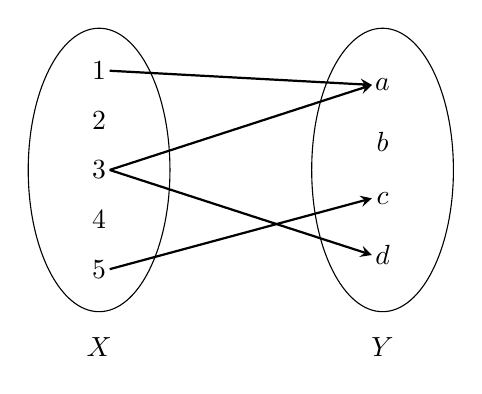
\begin{tikzpicture}[scale=0.9]
\draw (-2,0) ellipse (1cm and 2cm);
\draw (2,0) ellipse (1cm and 2cm);
\draw[-stealth, thick] (-1.85,1.4) -- (1.85,1.2);
\draw[-stealth, thick] (-1.85,0) -- (1.85,1.2);
\draw[-stealth, thick] (-1.85,0) -- (1.85,-1.2);
\draw[-stealth, thick] (-1.85,-1.4) -- (1.85,-0.4);
\draw (-2,-2.5) node {$X$} (2,-2.5) node {$Y$}
(-2,1.4) node {$1$} (-2,0.7) node {$2$} (-2,0) node {$3$}
(-2,-0.7) node {$4$} (-2,-1.4) node {$5$}
(2,1.2) node {$a$} (2,0.4) node {$b$} (2,-0.4) node {$c$} (2,-1.2) node {$d$};
\end{tikzpicture}

\small 对应 $f$
\end{minipage}
\hfill
\begin{minipage}{0.47\textwidth}
\centering
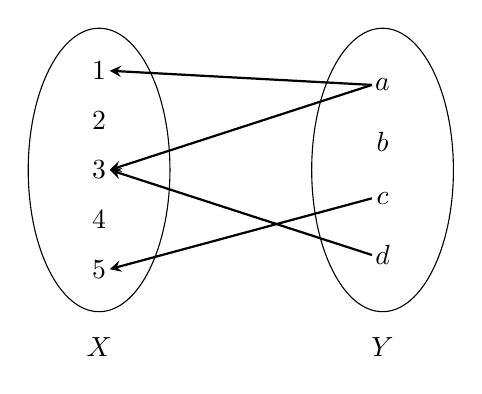
\begin{tikzpicture}[scale=0.9]
\draw (-2,0) ellipse (1cm and 2cm);
\draw (2,0) ellipse (1cm and 2cm);
\draw[stealth-, thick] (-1.85,1.4) -- (1.85,1.2);
\draw[stealth-, thick] (-1.85,0) -- (1.85,1.2);
\draw[stealth-, thick] (-1.85,0) -- (1.85,-1.2);
\draw[stealth-, thick] (-1.85,-1.4) -- (1.85,-0.4);
\draw (-2,-2.5) node {$X$} (2,-2.5) node {$Y$}
(-2,1.4) node {$1$} (-2,0.7) node {$2$} (-2,0) node {$3$}
(-2,-0.7) node {$4$} (-2,-1.4) node {$5$}
(2,1.2) node {$a$} (2,0.4) node {$b$} (2,-0.4) node {$c$} (2,-1.2) node {$d$};
\end{tikzpicture}

\small 逆对应 $f^{-1}$
\end{minipage}
\caption{对应 $f$ 与逆对应 $f^{-1}$ 的箭头图}
\label{fig:corr-arrow}
\end{figure}
\end{instance}

\begin{definition}[表格表示]\label{def:corr-table}
设 $f$ 是从集合 $X$ 到集合 $Y$ 的对应. 以 $X$ 的元素标记表格的各行, 以 $Y$ 的元素标记各列. 对 $x\in X$ 和 $y\in Y$, 当且仅当
\[
 (x,y)\in\Gamma_f
\]
时, 在第 $x$ 行、第 $y$ 列的格子中作一个标记. 这样得到的表格称为对应 $f$ 的{\color{blue}表格表示 (tabular representation)}.
\end{definition}

\begin{instance}
定义~\ref{def:corr-arrow-diagram} 后面的例子中的对应 $f$ 以及逆对应 $f^{-1}$ 可以分别表示为下表. 可以看出, 逆对应 $f^{-1}$ 的表格正是对应 $f$ 的表格的转置.
\begin{table}[H]
\centering
\begin{minipage}{0.47\textwidth}
\centering
\begin{tabular}{|c|c|c|c|c|}
\hline
 & $a$ & $b$ & $c$ & $d$\\
\hline
$1$ & $\checkmark$ & & & \\
\hline
$2$ & & & & \\
\hline
$3$ & $\checkmark$ & & & $\checkmark$\\
\hline
$4$ & & & & \\
\hline
$5$ & & & $\checkmark$ & \\
\hline
\end{tabular}

\small 对应 $f$
\end{minipage}
\hfill
\begin{minipage}{0.47\textwidth}
\centering
\begin{tabular}{|c|c|c|c|c|c|}
\hline
 & $1$ & $2$ & $3$ & $4$ & $5$\\
\hline
$a$ & $\checkmark$ & & $\checkmark$ & & \\
\hline
$b$ & & & & & \\
\hline
$c$ & & & & & $\checkmark$\\
\hline
$d$ & & & $\checkmark$ & & \\
\hline
\end{tabular}

\small 逆对应 $f^{-1}$
\end{minipage}
\caption{对应 $f$ 与逆对应 $f^{-1}$ 的表格表示}
\label{tab:corr-table}
\end{table}
\end{instance}

\begin{concept}\label{con:corr-03}
对于图~\ref{fig:corr-arrow} 左侧的对应 $f$, 只根据箭头图分别回答:
\begin{enumerate}[label=\rm(\arabic*)]
  \item 哪些起始集元素没有箭头发出?
  \item 哪些目标集元素没有箭头指向?
  \item 哪个起始集元素有两条不同的箭头发出? 这两条箭头分别指向哪里?
  \item 哪个目标集元素有两条不同的箭头指向? 这两条箭头分别来自哪里?
\end{enumerate}
\end{concept}

\begin{solution}
$2,4$ 没有箭头发出; $b$ 没有箭头指向; 从 $3$ 发出两条不同的箭头, 分别指向 $a,d$; 有两条不同的箭头指向 $a$, 分别来自 $1,3$.

\end{solution}

\begin{definition}[坐标平面图]\label{def:corr-coordinate-graph}
设 $X,Y$ 都是 $\mathbb R$ 的子集, $f$ 是从 $X$ 到 $Y$ 的对应. 此时
\[
 \Gamma_f\subseteq X\times Y\subseteq\mathbb R\times\mathbb R.
\]
把每个 $(x,y)\in\Gamma_f$ 看成坐标平面中坐标为 $(x,y)$ 的点, 并把这些点画在坐标平面中. 所得到的几何图形称为对应 $f$ 的{\color{blue}坐标平面图 (coordinate-plane graph)}.

要注意, $\Gamma_f$ 本身是定义对应 $f$ 的集合, 称为 $f$ 的图像; 坐标平面图则是这个集合在坐标平面中的几何表示.
\end{definition}

\begin{instance}
设 $f$ 是从 $\mathbb R$ 到 $\mathbb R$ 的对应, 其图像为
\[
 \Gamma_f:=\{(x,y)\in\mathbb R\times\mathbb R\mid x=y^2\}.
\]
它的坐标平面图是开口向右的抛物线. 逆对应 $f^{-1}$ 的图像由交换两个坐标得到,
\[
 \Gamma_{f^{-1}}
 =\{(x,y)\in\mathbb R\times\mathbb R\mid y=x^2\},
\]
所以它的坐标平面图是开口向上的抛物线.

\begin{figure}[H]
\centering
\begin{minipage}{0.45\textwidth}
\centering
\begin{tikzpicture}[scale=0.75]
\draw[-stealth] (-0.5,0)--(4.8,0) node[right] {$x$};
\draw[-stealth] (0,-2.6)--(0,2.6) node[above] {$y$};
\draw[thick,domain=-2:2,samples=100,smooth] plot ({\x*\x},{\x});
\node[below] at (2,-2.7) {$\Gamma_f:\ x=y^2$};
\end{tikzpicture}
\end{minipage}
\hfill
\begin{minipage}{0.45\textwidth}
\centering
\begin{tikzpicture}[scale=0.75]
\draw[-stealth] (-2.6,0)--(2.6,0) node[right] {$x$};
\draw[-stealth] (0,-0.5)--(0,4.8) node[above] {$y$};
\draw[thick,domain=-2:2,samples=100,smooth] plot ({\x},{\x*\x});
\node[below] at (0,-0.7) {$\Gamma_{f^{-1}}:\ y=x^2$};
\end{tikzpicture}
\end{minipage}
\caption{对应 $f$ 与逆对应 $f^{-1}$ 的坐标平面图}
\label{fig:corr-coordinate-graph}
\end{figure}
\end{instance}

\begin{exercise}\label{ex:corr-representation}
设 $X=\{1,2,3\}$, $Y=\{a,b,c\}$, 对应 $f$ 的图像为
\[
 \Gamma_f=\{(1,a),(1,c),(3,b)\}.
\]
画出 $f$ 的箭头图并写出相应的表格, 然后不重新计算图像, 直接写出逆对应 $f^{-1}$ 的表格.
\end{exercise}

\section{像与原像}

对应的图像记录了哪些元素彼此配对. 一旦给定图像中的一对 $(x,y)$, 既可以固定第一个坐标 $x$ 去寻找与它配对的第二个坐标, 也可以固定第二个坐标 $y$ 反向寻找与它配对的第一个坐标. 下面的定义分别给这两种关系命名, 并进一步把它们推广到同时寻找多个元素的配对元素的情形.

\begin{definition}[像与原像]\label{def:corr-image-preimage}
设 $X$ 和 $Y$ 为两个集合, $f$ 为从 $X$ 到 $Y$ 的对应.
\begin{enumerate}[label=\rm(\arabic*)]
  \item 若 $(x,y)\in\Gamma_f$, 称 $y$ 是 $x$ 在 $f$ 下的一个{\color{blue}像 (image)}, 称 $x$ 是 $y$ 在 $f$ 下的一个{\color{blue}原像 (preimage)}.
  \item 对任意集合 $A$, 定义
  \[
   f(A):=\{y\in Y\mid \exists\,x\in A,\ (x,y)\in\Gamma_f\},
  \]
  称为 $A$ 在 $f$ 下的{\color{blue}像}.
  \item 对任意集合 $B$, 定义
  \[
   f^{-1}(B):=\{x\in X\mid \exists\,y\in B,\ (x,y)\in\Gamma_f\},
  \]
  称为 $B$ 在 $f$ 下的{\color{blue}原像}.
\end{enumerate}
这里的 $f^{-1}(B)$ 正是集合 $B$ 在逆对应 $f^{-1}$ 下的像.
\end{definition}

\begin{concept}\label{con:corr-04}
对图~\ref{fig:corr-arrow} 中的对应, 求
\[
 f(\{1,3\}),\qquad
 f^{-1}(\{a,c\}),\qquad
 f(\varnothing),\qquad
 f^{-1}(\varnothing).
\]
\end{concept}

\begin{solution}
\[
 f(\{1,3\})=\{a,d\},\qquad
 f^{-1}(\{a,c\})=\{1,3,5\},
\]
且空集的像、原像都是空集.
\end{solution}

\begin{definition}[定义域与值域]\label{def:corr-domain-image}
设 $f$ 为对应. 定义
\[
 \operatorname{Dom}(f):=f^{-1}(\mathscr A_f),
 \qquad
 \operatorname{Ran}(f):=f(\mathscr D_f).
\]
分别称为 $f$ 的{\color{blue}定义域 (domain)}和{\color{blue}值域 (range)}.

因此, $\operatorname{Dom}(f)$ 是起始集中至少有一个像的元素组成的集合, $\operatorname{Ran}(f)$ 是目标集中至少有一个原像的元素组成的集合. 我们总有
\[
 \operatorname{Dom}(f)\subseteq\mathscr D_f,
 \qquad
 \operatorname{Ran}(f)\subseteq\mathscr A_f.
\]
并且
\[
 \operatorname{Dom}(f)=\operatorname{Ran}(f^{-1}),
 \qquad
 \operatorname{Ran}(f)=\operatorname{Dom}(f^{-1}).
\]
\end{definition}

\begin{concept}\label{con:corr-05}
设 $f$ 是从 $\{1,2,3,4\}$ 到 $\{a,b,c\}$ 的对应, 且
\[
 \Gamma_f=\{(1,a),(1,b),(3,b)\}.
\]
求 $\operatorname{Dom}(f)$ 与 $\operatorname{Ran}(f)$, 并指出哪些元素属于起始集但不属于定义域, 哪些元素属于目标集但不属于值域.
\end{concept}

\begin{solution}
\[
 \operatorname{Dom}(f)=\{1,3\},\qquad
 \operatorname{Ran}(f)=\{a,b\}.
\]
$2,4$ 属于起始集但不属于定义域, $c$ 属于目标集但不属于值域.
\end{solution}

\begin{instance}
设 $f$ 是从 $\mathbb R$ 到 $\mathbb R$ 的对应, 图像为
\[
 \Gamma_f:=\{(x,y)\in\mathbb R\times\mathbb R\mid x^2+y^2\leq1\}.
\]
则
\[
 \operatorname{Dom}(f)=\{x\in\mathbb R\mid -1\leq x\leq1\},
\]
且
\[
 \operatorname{Ran}(f)=\{y\in\mathbb R\mid -1\leq y\leq1\}.
\]
\end{instance}

\begin{proposition}\label{prop:corr-monotone}
设 $f$ 为对应.
\begin{enumerate}[label=\rm(\arabic*)]
  \item 若 $A'\subseteq A$, 则 $f(A')\subseteq f(A)$;
  \item 若 $B'\subseteq B$, 则 $f^{-1}(B')\subseteq f^{-1}(B)$.
\end{enumerate}
\end{proposition}

\begin{proof}
若 $y\in f(A')$, 则存在 $x\in A'$ 使得 $(x,y)\in\Gamma_f$. 由 $A'\subseteq A$, 有 $x\in A$, 从而 $y\in f(A)$. 第一个命题成立. 对逆对应 $f^{-1}$ 应用第一个命题即得到第二个命题.
\end{proof}

\begin{exercise}\label{ex:corr-monotone}
\begin{enumerate}[label=\rm(\arabic*)]
  \item 对于一个具体的对应验证命题~\ref{prop:corr-monotone}.
  \item 若删去 $A'\subseteq A$ 的假设, 能否仍总是保证 $f(A')\subseteq f(A)$? 给出反例.
  \item 反过来, 从 $f(A')\subseteq f(A)$ 能否推出 $A'\subseteq A$? 给出反例.
\end{enumerate}
\end{exercise}

\begin{proposition}\label{prop:corr-domain-image-duality}
对任意对应 $f$,
\[
 \operatorname{Ran}(f)=f(\operatorname{Dom}(f)),
 \qquad
 \operatorname{Dom}(f)=f^{-1}(\operatorname{Ran}(f)).
\]
\end{proposition}

\begin{proof}
由 $\operatorname{Dom}(f)\subseteq\mathscr D_f$ 和命题~\ref{prop:corr-monotone},
\[
 f(\operatorname{Dom}(f))\subseteq f(\mathscr D_f)=\operatorname{Ran}(f).
\]
反过来, 若 $y\in\operatorname{Ran}(f)$, 存在 $x\in\mathscr D_f$ 使得 $(x,y)\in\Gamma_f$. 此时 $x\in\operatorname{Dom}(f)$, 所以 $y\in f(\operatorname{Dom}(f))$. 第一个等式成立. 对逆对应运用第一个等式即可得到第二个等式.
\end{proof}

\begin{exercise}\label{ex:corr-domain-image-duality}
设 $A\subseteq\mathscr D_f$. 是否总有
\[
 f(A)=f(A\cap\operatorname{Dom}(f))?
\]
证明或否定这个命题. 类似地写出并证明一个关于 $f^{-1}(B)$ 与 $\operatorname{Ran}(f)$ 的公式.
\end{exercise}

\begin{proposition}\label{prop:corr-image-criterion}
设 $f$ 为对应.
\begin{enumerate}[label=\rm(\arabic*)]
  \item 对任意集合 $A$ 和对象 $y$,
  \[
   y\in f(A)
   \quad\Leftrightarrow\quad
   A\cap f^{-1}(\{y\})\neq\varnothing;
  \]
  \item 对任意集合 $B$ 和对象 $x$,
  \[
   x\in f^{-1}(B)
   \quad\Leftrightarrow\quad
   B\cap f(\{x\})\neq\varnothing.
  \]
\end{enumerate}
\end{proposition}

\begin{proof}
第一个命题只是把``存在 $x\in A$ 使得 $(x,y)\in\Gamma_f$''改写成``存在 $x$ 同时属于 $A$ 和 $f^{-1}(\{y\})$''. 对逆对应运用第一个命题即可得到第二个命题.
\end{proof}

\begin{exercise}\label{ex:corr-image-criterion}
为什么命题~\ref{prop:corr-image-criterion} 中必须写单元素集合 $\{y\}$ 而不能直接写 $f^{-1}(y)$? 在目前的定义体系中, 后一个记号是否已经有意义?
\end{exercise}

\begin{proposition}\label{prop:corr-union-intersection}
设 $f$ 为对应, $I$ 为集合.
\begin{enumerate}[label=\rm(\arabic*)]
  \item 对集合族 $(A_i)_{i\in I}$,
  \[
   f\left(\bigcup_{i\in I}A_i\right)
   =\bigcup_{i\in I}f(A_i).
  \]
  若 $I\neq\varnothing$, 则
  \[
   f\left(\bigcap_{i\in I}A_i\right)
   \subseteq\bigcap_{i\in I}f(A_i).
  \]
  \item 对集合族 $(B_i)_{i\in I}$,
  \[
   f^{-1}\left(\bigcup_{i\in I}B_i\right)
   =\bigcup_{i\in I}f^{-1}(B_i).
  \]
  若 $I\neq\varnothing$, 则
  \[
   f^{-1}\left(\bigcap_{i\in I}B_i\right)
   \subseteq\bigcap_{i\in I}f^{-1}(B_i).
  \]
\end{enumerate}
\end{proposition}

\begin{proof}
先证明第一个命题中的并集公式, 对任意 $y$,
\[
 y\in f\left(\bigcup_{i\in I}A_i\right)
\]
当且仅当存在 $x$ 与 $i\in I$ 使得 $x\in A_i$ 且 $(x,y)\in\Gamma_f$, 这又当且仅当存在 $i\in I$ 使得 $y\in f(A_i)$.

若 $I\neq\varnothing$ 且 $A:=\bigcap_{i\in I}A_i$, 则对每个 $i\in I$ 都有 $A\subseteq A_i$. 由命题~\ref{prop:corr-monotone}, $f(A)\subseteq f(A_i)$ 对每个 $i$ 成立, 因此
\[
 f(A)\subseteq\bigcap_{i\in I}f(A_i).
\]
对逆对应 $f^{-1}$ 使用上述两条结论, 就得到关于原像的结论.
\end{proof}

\begin{exercise}\label{ex:corr-union-intersection}
\begin{enumerate}[label=\rm(\arabic*)]
  \item 构造一个对应 $f$ 和两个集合 $A_1,A_2$, 使
  \[
   f(A_1\cap A_2)\subset f(A_1)\cap f(A_2).
  \]
  \item 构造一个对应 $f$ 和两个集合 $B_1,B_2$, 使
  \[
   f^{-1}(B_1\cap B_2)\subset f^{-1}(B_1)\cap f^{-1}(B_2).
  \]
  \item 思考: 分别加入什么假设后, 上述两个包含关系可以升级为等式?
\end{enumerate}
\end{exercise}

\section{对应的复合}

如果 $x$ 先通过对应 $f$ 与某个 $y$ 相连, 而这个 $y$ 又通过对应 $g$ 与某个 $z$ 相连, 就可以把两步连接压缩成从 $x$ 到 $z$ 的一步连接. 这就是对应的复合. 对一般对应, 连接 $x$ 与 $z$ 的中间元素 $y$ 可能不唯一, 因而复合的定义必须使用存在量词.

\begin{definition}\label{def:corr-composition}
设 $f,g$ 为对应. 定义 $g$ 与 $f$ 的{\color{blue}复合对应 (composite correspondence)} $g\circ f$ 为从 $\mathscr D_f$ 到 $\mathscr A_g$ 的对应, 其图像为
\[
 \Gamma_{g\circ f}
 :=\{(x,z)\in\mathscr D_f\times\mathscr A_g\mid
 \exists\,y\in\mathscr A_f\cap\mathscr D_g,
 (x,y)\in\Gamma_f\ \text{且}\ (y,z)\in\Gamma_g\}.
\]
\end{definition}

\begin{concept}\label{con:corr-06}
设
\[
 \Gamma_f=\{(1,a),(1,b),(2,b)\},
 \qquad
 \Gamma_g=\{(a,u),(b,v)\}.
\]
其中 $f$ 是从 $\{1,2\}$ 到 $\{a,b\}$的对应, $g$ 是从 $\{a,b\}$ 到 $\{u,v\}$的对应. 求 $\Gamma_{g\circ f}$. 如果从 $\Gamma_g$ 中删去 $(b,v)$, 哪些复合配对会消失?
\end{concept}

\begin{solution}
\[
 \Gamma_{g\circ f}=\{(1,u),(1,v),(2,v)\}.
\]
删去 $(b,v)$ 后, $(1,v),(2,v)$ 消失.
\end{solution}

\begin{proposition}\label{prop:corr-inverse-composition}
对任意对应 $f,g$,
\[
 (g\circ f)^{-1}=f^{-1}\circ g^{-1}.
\]
\end{proposition}

\begin{proof}
对任意 $x\in\mathscr D_f$, $z\in\mathscr A_g$,
\[
 (z,x)\in\Gamma_{(g\circ f)^{-1}}
\]
当且仅当 $(x,z)\in\Gamma_{g\circ f}$, 即存在 $y$ 使得
\[
 (x,y)\in\Gamma_f,
 \qquad
 (y,z)\in\Gamma_g.
\]
这又等价于
\[
 (z,y)\in\Gamma_{g^{-1}},
 \qquad
 (y,x)\in\Gamma_{f^{-1}},
\]
即 $(z,x)\in\Gamma_{f^{-1}\circ g^{-1}}$.
\end{proof}

\begin{exercise}\label{ex:corr-inverse-composition}
解释为什么公式中的次序必须反转. 构造两个有限对应 $f,g$, 使 $g\circ f$ 有意义且 $f^{-1}\circ g^{-1}$ 非空, 并直接计算两边. 再说明一般不能把右边写成 $g^{-1}\circ f^{-1}$.
\end{exercise}

\begin{proposition}\label{prop:corr-associativity}
对任意对应 $f,g,h$,
\[
 h\circ(g\circ f)=(h\circ g)\circ f.
\]
\end{proposition}

\begin{proof}
对任意 $(x,w)$, 它属于 $h\circ(g\circ f)$ 的图像, 当且仅当存在 $y,z$ 使得
\[
 (x,y)\in\Gamma_f,
 \qquad
 (y,z)\in\Gamma_g,
 \qquad
 (z,w)\in\Gamma_h.
\]
而这正是 $(x,w)$ 属于 $(h\circ g)\circ f$ 的图像的条件. 两边起始集和目标集也相同, 因而两个对应相等.
\end{proof}

\begin{exercise}\label{ex:corr-associativity}
结合律说明三个对应复合时可以省略括号. 但能否交换复合次序? 构造 $f,g$ 使 $g\circ f\neq f\circ g$, 或说明在你的例子中为何其中一个复合甚至为空对应.
\end{exercise}

\begin{proposition}\label{prop:corr-identity-composition}
若 $f$ 是从 $X$ 到 $Y$ 的对应, 则
\[
 f\circ\operatorname{Id}_X=f
 =\operatorname{Id}_Y\circ f.
\]
\end{proposition}

\begin{proof}
$(x,y)$ 属于 $f\circ\operatorname{Id}_X$ 的图像, 当且仅当存在 $x'$ 使得 $(x,x')\in\Delta_X$ 且 $(x',y)\in\Gamma_f$. 第一个条件强制 $x'=x$, 因而这等价于 $(x,y)\in\Gamma_f$. 另一个等式同理, 或对第一个等式取逆并利用命题~\ref{prop:corr-inverse-composition}.
\end{proof}

\begin{exercise}\label{ex:corr-identity-composition}
若 $Z$ 是严格包含 $X$ 的集合, 把 $\operatorname{Id}_X$ 换成 $\operatorname{Id}_Z$ 后, 公式 $f\circ\operatorname{Id}_Z=f$ 是否仍能直接成立? 先检查复合对应的起始集, 再说明问题所在.
\end{exercise}

\begin{proposition}\label{prop:corr-composition-image}
设 $f,g$ 为对应. 对任意集合 $A,B$,
\[
 (g\circ f)(A)=g(f(A)),
\]
以及
\[
 (g\circ f)^{-1}(B)=f^{-1}(g^{-1}(B)).
\]
特别地,
\[
 \operatorname{Ran}(g\circ f)=g(\operatorname{Ran}(f))\subseteq\operatorname{Ran}(g),
\]
且
\[
 \operatorname{Dom}(g\circ f)=f^{-1}(\operatorname{Dom}(g))\subseteq\operatorname{Dom}(f).
\]
若 $\operatorname{Dom}(g)\subseteq\operatorname{Ran}(f)$, 则
\[
 \operatorname{Ran}(g\circ f)=\operatorname{Ran}(g).
\]
若 $\operatorname{Ran}(f)\subseteq\operatorname{Dom}(g)$, 则
\[
 \operatorname{Dom}(g\circ f)=\operatorname{Dom}(f).
\]
\end{proposition}

\begin{proof}
$z\in(g\circ f)(A)$ 当且仅当存在 $x\in A$ 和 $y$ 使得
\[
 (x,y)\in\Gamma_f,
 \qquad
 (y,z)\in\Gamma_g.
\]
这等价于存在 $y\in f(A)$ 使得 $(y,z)\in\Gamma_g$, 即 $z\in g(f(A))$. 将复合对应的像公式用于逆对应, 利用命题~\ref{prop:corr-inverse-composition} 得到复合对应的原像公式.

令 $A=\mathscr D_f$, 即得
\[
 \operatorname{Ran}(g\circ f)=g(\operatorname{Ran}(f))\subseteq\operatorname{Ran}(g).
\]
若 $\operatorname{Dom}(g)\subseteq\operatorname{Ran}(f)$, 则由命题~\ref{prop:corr-domain-image-duality} 与单调性,
\[
 \operatorname{Ran}(g)=g(\operatorname{Dom}(g))
 \subseteq g(\operatorname{Ran}(f))
 =\operatorname{Ran}(g\circ f).
\]
从而得到等号. 关于定义域部分可由复合对应的原像公式同理得到.
\end{proof}

\begin{exercise}\label{ex:corr-composition-image}
\begin{enumerate}[label=\rm(\arabic*)]
  \item 构造 $f,g$, 使 $\operatorname{Ran}(g\circ f)$ 严格包含于 $\operatorname{Ran}(g)$.
  \item 在你的例子中指出 $\operatorname{Dom}(g)\subseteq\operatorname{Ran}(f)$ 为什么失败.
  \item 构造一个例子说明: 即使 $\operatorname{Ran}(g\circ f)=\operatorname{Ran}(g)$, 也不一定能推出 $\operatorname{Dom}(g)\subseteq\operatorname{Ran}(f)$.
\end{enumerate}
\end{exercise}

\section{满对应与多值映射}

定义域和值域分别记录``哪些出发元素至少有一个像''和``哪些到达元素至少有一个原像''. 因而把这两个集合分别要求等于整个起始集或目标集, 就得到两类重要性质. 它们互相通过取逆对应交换.

\begin{definition}[满对应与多值映射]\label{def:corr-surjective-multivalued}
设 $f$ 为对应.
\begin{enumerate}[label=\rm(\arabic*)]
  \item 若目标集中的每个元素都至少有一个原像, 即
  \[
   \operatorname{Ran}(f)=\mathscr A_f,
  \]
  则称 $f$ 为{\color{blue}满对应 (surjective correspondence)}. 
  \item 若起始集中的每个元素都至少有一个像, 即
  \[
   \operatorname{Dom}(f)=\mathscr D_f,
  \]
  则称 $f$ 为{\color{blue}多值映射 (multivalued map)}.
\end{enumerate}
因此, $f$ 是多值映射当且仅当 $f^{-1}$ 是满对应.
\end{definition}

\begin{concept}\label{con:corr-07}
观察图~\ref{fig:corr-arrow} 中的对应. 它是满对应吗? 是多值映射吗? 如果要只增加一条箭头使它成为满对应, 应怎样增加? 如果要使它成为多值映射, 至少还需要增加几条箭头?
\end{concept}

\begin{solution}
图~\ref{fig:corr-arrow} 中 $b$ 无原像, 故不是满对应; $2,4$ 无像, 故不是多值映射. 使其成为满对应只需增加一条指向 $b$ 的箭头; 使其成为多值映射至少需要给 $2,4$ 各补一条箭头.
\end{solution}

\begin{proposition}\label{prop:corr-surj-multi-closures}
设 $f$ 为对应.
\begin{enumerate}[label=\rm(\arabic*)]
  \item 对任意 $B\subseteq\operatorname{Ran}(f)$,
  \[
   B\subseteq f(f^{-1}(B)).
  \]
  \item 对任意 $A\subseteq\operatorname{Dom}(f)$,
  \[
   A\subseteq f^{-1}(f(A)).
  \]
\end{enumerate}
\end{proposition}

\begin{proof}
若 $y\in B$, 则 $y\in\operatorname{Ran}(f)$, 所以存在 $x$ 使得 $(x,y)\in\Gamma_f$. 于是 $x\in f^{-1}(B)$, 从而 $y\in f(f^{-1}(B))$. 对逆对应运用第一个命题即可得到第二个命题.
\end{proof}

\begin{exercise}\label{ex:corr-surj-multi-closures}
设 $B\subseteq\mathscr A_f$. 证明
\[
 B\subseteq f(f^{-1}(B))
 \quad\Leftrightarrow\quad
 B\subseteq\operatorname{Ran}(f).
\]
类似地, 对 $A\subseteq\mathscr D_f$, 写出并证明相应的等价关系.
\end{exercise}

\begin{proposition}\label{prop:corr-surj-from-composite}
设 $f,g$ 为对应.
\begin{enumerate}[label=\rm(\arabic*)]
  \item 若 $g\circ f$ 是满对应, 则 $g$ 是满对应;
  \item 若 $g\circ f$ 是多值映射, 则 $f$ 是多值映射.
\end{enumerate}
\end{proposition}

\begin{proof}
由命题~\ref{prop:corr-composition-image},
\[
 \operatorname{Ran}(g\circ f)\subseteq\operatorname{Ran}(g)\subseteq\mathscr A_g.
\]
而 $\mathscr A_{g\circ f}=\mathscr A_g$. 若 $g\circ f$ 是满对应, 则 $\operatorname{Ran}(g\circ f)=\mathscr A_g$, 从而 $\operatorname{Ran}(g)=\mathscr A_g$. 对逆对应运用第一个命题, 并利用命题~\ref{prop:corr-inverse-composition}, 即可得到第二个命题.
\end{proof}

\begin{exercise}\label{ex:corr-surj-from-composite}
命题~\ref{prop:corr-surj-from-composite} 的逆命题一般不成立. 构造 $g$ 是满对应而 $g\circ f$ 不是满对应的例子, 并指出失败原因. 再给出一个 $f$ 是多值映射但 $g\circ f$ 不是多值映射的例子.
\end{exercise}

\begin{proposition}\label{prop:corr-composite-surj}
设 $f,g$ 为对应.
\begin{enumerate}[label=\rm(\arabic*)]
  \item 若 $g$ 是满对应且
  \[
   \operatorname{Dom}(g)\subseteq\operatorname{Ran}(f),
  \]
  则 $g\circ f$ 是满对应.
  \item 若 $f$ 是多值映射且
  \[
   \operatorname{Ran}(f)\subseteq\operatorname{Dom}(g),
  \]
  则 $g\circ f$ 是多值映射.
\end{enumerate}
\end{proposition}

\begin{proof}
由命题~\ref{prop:corr-composition-image}, 第一个命题的附加假设给出
\[
 \operatorname{Ran}(g\circ f)=\operatorname{Ran}(g)=\mathscr A_g,
\]
所以 $g\circ f$ 是满对应. 对逆对应运用第一个命题, 并利用命题~\ref{prop:corr-inverse-composition}, 即可得到第二个命题.
\end{proof}

\begin{exercise}\label{ex:corr-composite-surj}
分别构造例子说明命题~\ref{prop:corr-composite-surj} 中的两个集合包含假设不能简单删去. 再假设 $\mathscr A_f=\mathscr D_g$. 若 $g$ 是多值映射, 说明第二个命题中的包含关系为何自动成立; 若 $f$ 是满对应, 说明第一个命题中的包含关系为何自动成立.
\end{exercise}

\section{函数与单对应}

前一节要求的是``至少一个''. 另一类基本问题是``至多一个'': 一个起始元素是否会同时连向两个不同元素? 一个目标元素是否会同时来自两个不同元素? 第一个唯一性条件给出函数, 第二个唯一性条件给出单对应; 这两种唯一性条件通过逆对应互换.

\begin{definition}[函数与单对应]\label{def:corr-single-injective}
设 $f$ 为对应.
\begin{enumerate}[label=\rm(\arabic*)]
  \item 如果 $\mathscr D_f$ 中每个元素在 $f$ 下至多有一个像, 称 $f$ 为{\color{blue}函数 (function)}.
  \item 如果 $\mathscr A_f$ 中每个元素在 $f$ 下至多有一个原像, 称 $f$ 为{\color{blue}单对应 (injective correspondence)}.
\end{enumerate}
因此, $f$ 是单对应当且仅当 $f^{-1}$ 是函数.
\end{definition}

\begin{concept}\label{con:corr-08}
对下列三种箭头情形分别判断是否违反函数的定义或单对应的定义:
\begin{enumerate}[label=\rm(\arabic*)]
  \item 同一个 $x$ 指向两个不同的 $y$;
  \item 两个不同的 $x$ 指向同一个 $y$;
  \item 某个 $x$ 没有任何像.
\end{enumerate}
特别说明第 (3) 种情况为什么不妨碍一个对应成为函数.
\end{concept}

\begin{solution}
(1) 违反函数的定义; (2) 违反单对应的定义; (3) 不违反函数的定义, 因为``至多一个''允许零个像.
\end{solution}

\begin{notation}[函数的值]\label{not:corr-value}
若 $f$ 是函数且 $x\in\operatorname{Dom}(f)$, 则 $x$ 有唯一的像. 记这个像为
\[
 f(x).
\]
我们也用
\[
 x\longmapsto f(x)
\]
表示 $f(x)$ 是 $x$ 在 $f$ 下唯一的像.
要注意, 若 $x\notin\operatorname{Dom}(f)$, 则 $f(x)$ 没有定义.
\end{notation}

\begin{proposition}\label{prop:corr-ffinverse}
设 $f$ 为对应.
\begin{enumerate}[label=\rm(\arabic*)]
  \item 若 $f$ 是单对应, 则对任意集合 $A$,
  \[
   f^{-1}(f(A))\subseteq A.
  \]
  \item 若 $f$ 是函数, 则对任意集合 $B$,
  \[
   f(f^{-1}(B))\subseteq B.
  \]
\end{enumerate}
\end{proposition}

\begin{proof}
若 $x\in f^{-1}(f(A))$, 存在 $y\in f(A)$ 使得 $(x,y)\in\Gamma_f$. 又因 $y\in f(A)$, 存在 $x'\in A$ 使得 $(x',y)\in\Gamma_f$. 由 $f$ 是单对应, $y$ 至多有一个原像, 故 $x=x'\in A$. 对逆对应运用第一个命题即可得到第二个命题.
\end{proof}

\begin{exercise}\label{ex:corr-ffinverse}
\begin{enumerate}[label=\rm(\arabic*)]
  \item 若 $f$ 同时是单对应和多值映射, 对 $A\subseteq\mathscr D_f$ 能否得到 $f^{-1}(f(A))=A$? 说明理由.
  \item 若删去单对应假设, 构造严格包含 $A\subset f^{-1}(f(A))$ 的例子.
  \item 若删去``$f$ 是函数''这一假设, 可否构造严格包含 $B\subset f(f^{-1}(B))$ 的例子? 
\end{enumerate}
\end{exercise}

\begin{proposition}\label{prop:corr-composite-single-injective}
设 $f,g$ 为对应.
\begin{enumerate}[label=\rm(\arabic*)]
  \item 若 $f,g$ 都是函数, 则 $g\circ f$ 是函数. 对任意 $x\in\operatorname{Dom}(g\circ f)$,
  \[
   (g\circ f)(x)=g(f(x)).
  \]
  \item 若 $f,g$ 都是单对应, 则 $g\circ f$ 是单对应.
\end{enumerate}
\end{proposition}

\begin{proof}
设 $x$ 在 $g\circ f$ 下有像 $z,z'$. 则存在 $y,y'$ 使得
\[
 (x,y),(x,y')\in\Gamma_f,
 \qquad
 (y,z),(y',z')\in\Gamma_g.
\]
因 $f$ 是函数, $y=y'=f(x)$; 因 $g$ 是函数, $z=z'=g(f(x))$. 故 $g$ 和 $f$ 的复合是函数, 并且公式 $(g\circ f)(x)=g(f(x))$ 成立. 对逆对应运用第一个命题, 并利用命题~\ref{prop:corr-inverse-composition}, 即可得到第二个命题.
\end{proof}

\begin{exercise}\label{ex:corr-composite-single-injective}
如果只知道 $g\circ f$ 是函数, 能否推出 $f$ 或 $g$ 是函数? 分别构造反例. 同样讨论``$g\circ f$ 是单对应''能否推出 $f$ 或 $g$ 是单对应.
\end{exercise}

\begin{proposition}\label{prop:corr-inj-from-composite}
设 $f,g$ 为对应.
\begin{enumerate}[label=\rm(\arabic*)]
  \item 若 $g\circ f$ 是单对应且
  \[
   \operatorname{Ran}(f)\subseteq\operatorname{Dom}(g),
  \]
  则 $f$ 是单对应.
  \item 若 $g\circ f$ 是函数且
  \[
   \operatorname{Dom}(g)\subseteq\operatorname{Ran}(f),
  \]
  则 $g$ 是函数.
\end{enumerate}
\end{proposition}

\begin{proof}
设 $y\in\operatorname{Ran}(f)$, 且 $x,x'$ 都是 $y$ 的原像. 由 $\operatorname{Ran}(f)\subseteq\operatorname{Dom}(g)$, $y$ 至少有一个 $g$-像 $z$. 则 $(x,z)$ 和 $(x',z)$ 都属于 $g\circ f$ 的图像. 因复合是单对应, $x=x'$. 故 $f$ 是单对应. 对逆对应运用第一个命题, 并利用命题~\ref{prop:corr-inverse-composition}, 即可得到第二个命题.
\end{proof}

\begin{exercise}\label{ex:corr-inj-from-composite}
说明命题~\ref{prop:corr-inj-from-composite} 中的包含假设确实有作用: 构造 $g\circ f$ 是单对应但 $f$ 不是单对应的例子, 并使失败恰好来自包含关系 $\operatorname{Ran}(f)\subseteq\operatorname{Dom}(g)$ 不成立.
\end{exercise}

\begin{proposition}\label{prop:corr-intersection-uniqueness}
设 $I$ 是非空集合.
\begin{enumerate}[label=\rm(\arabic*)]
  \item 若 $f$ 是函数, 则对任意集合族 $(B_i)_{i\in I}$,
  \[
   f^{-1}\left(\bigcap_{i\in I}B_i\right)
   =\bigcap_{i\in I}f^{-1}(B_i).
  \]
  \item 若 $f$ 是单对应, 则对任意集合族 $(A_i)_{i\in I}$,
  \[
   f\left(\bigcap_{i\in I}A_i\right)
   =\bigcap_{i\in I}f(A_i).
  \]
\end{enumerate}
\end{proposition}

\begin{proof}
对于一般对应已经由命题~\ref{prop:corr-union-intersection} 给出``$\subseteq$''方向. 设 $x\in\bigcap_{i\in I}f^{-1}(B_i)$. 

对每个 $i\in I$, 元素 $x$ 至少有一个像落在 $B_i$ 中. 由于 $f$ 是函数, 这些像必须都是同一个 $f(x)$, 因而 $f(x)$ 属于每个 $B_i$, 即 $x\in f^{-1}(\bigcap_iB_i)$. 所以第一个等式成立. 对逆对应运用第一个等式即可得到第二个等式.
\end{proof}

\begin{exercise}\label{ex:corr-intersection-uniqueness}
分别给出例子说明: 若 $f$ 不是函数, 第一个等式可能失败; 若 $f$ 不是单对应, 第二个等式可能失败. 你的例子应尽可能只含少量元素.
\end{exercise}

\section{映射与双射}

函数只要求起始集中的每个元素``至多''有一个像, 因而函数的定义域可以严格小于它的起始集. 多值映射则要求起始集中的每个元素``至少''有一个像. 因此, 一个对应同时是函数和多值映射时, 起始集中的每个元素恰好有一个像; 我们把这样的函数称为映射. 在映射的框架中, 单对应和满对应分别成为熟悉的单射与满射.

\begin{definition}[映射]\label{def:corr-mapping}
若函数 $f$ 同时是多值映射, 即它的定义域等于起始集, 则称 $f$ 为{\color{blue}映射 (map)}. 换言之, 映射就是起始集中的每个元素都有唯一像的函数.

若 $f$ 是从 $X$ 到 $Y$ 的映射, 则记
\[
 f:X\longrightarrow Y.
\]
此时 $\operatorname{Dom}(f)=X$, 因而对每个 $x\in X$ 都定义了唯一的 $f(x)\in Y$.
\end{definition}

\begin{notation}[映射的像]\label{not:corr-mapping-image}
对一般对应, 我们仍使用定义~\ref{def:corr-domain-image} 中的记号
\[
 \operatorname{Ran}(f)
\]
表示值域. 当 $f:X\to Y$ 是映射时, 按照代数中更常用的习惯, 把这个集合记作
\[
 \operatorname{Im}(f)
 :=\operatorname{Ran}(f)
 =\{f(x)\mid x\in X\},
\]
并称之为 $f$ 的{\color{blue}像}. 因此
\[
 \operatorname{Im}(f)\subseteq Y.
\]
本书从这里起约定: 对一般对应使用 $\operatorname{Ran}(f)$; 对映射优先使用 $\operatorname{Im}(f)$.
\end{notation}

\begin{concept}\label{con:corr-09}
判断下列对应是否为映射:
\begin{enumerate}[label=\rm(\arabic*)]
  \item 每个起始元素恰有一个箭头发出, 但两个不同元素可以指向同一个到达元素;
  \item 每个起始元素至多有一个箭头发出, 其中一个元素没有箭头;
  \item 每个起始元素至少有一个箭头发出, 其中一个元素发出两条箭头.
\end{enumerate}
\end{concept}

\begin{solution}
只有 (1) 是映射. (2) 缺少``至少一个像''的条件, (3) 缺少``至多一个像''的条件.
\end{solution}

\begin{notation}[映射集合]\label{not:corr-mapping-space}
设 $X,Y$ 为集合. 所有从 $X$ 到 $Y$ 的映射组成的集合记作
\[
 Y^X.
\]
一个元素 $u\in Y^X$ 也可以写成以 $X$ 为指标的一族 $Y$ 中的元素
\[
 (u(x))_{x\in X}.
\]
若 $E_n:=\{1,\ldots,n\}$, 则映射 $u:E_n\to Y$ 与 $n$ 元组
\[
 (u(1),\ldots,u(n))
\]
自然对应, 因而这里的 $Y^{E_n}$ 可与第二章的 Cartesian 幂 $Y^n$ 等同起来.
\end{notation}

\begin{instance}
恒等对应 $\operatorname{Id}_X$ 是映射, 称为 $X$ 上的{\color{blue}恒等映射 (identity map)}. 若 $y_0\in Y$, 把每个 $x\in X$ 都指向 $y_0$ 的映射称为以 $y_0$ 为值的 {\color{blue}常值映射 (constant map)}.
\end{instance}

\begin{proposition}\label{prop:corr-composition-mappings}
若 $f:X\to Y$ 和 $g:Y\to Z$ 是映射, 则 $g\circ f$ 是从 $X$ 到 $Z$ 的映射, 且
\[
 (g\circ f)(x)=g(f(x))
\]
对每个 $x\in X$ 成立.
\end{proposition}

\begin{proof}
映射 $f,g$ 都是函数, 故由命题~\ref{prop:corr-composite-single-injective}, $g\circ f$ 是函数. 又 $\operatorname{Im}(f)\subseteq Y=\operatorname{Dom}(g)$, 且 $f$ 是多值映射, 由命题~\ref{prop:corr-composite-surj} 的第二个命题, $g\circ f$ 是多值映射. 因而它是映射. 值公式已在命题~\ref{prop:corr-composite-single-injective} 中证明.
\end{proof}

\begin{exercise}\label{ex:corr-composition-mappings}
设 $f(x)=3x+1$, $g(x)=x^2-1$ 是从 $\mathbb R$ 到 $\mathbb R$ 的映射. 求 $f\circ g$ 与 $g\circ f$, 并判断二者是否相等. 这个例子说明复合具有结合律但一般不具有交换律.
\end{exercise}

\begin{definition}[单射、满射与双射]\label{def:corr-inj-surj-bij}
设 $f:X\to Y$ 为映射.
\begin{enumerate}[label=\rm(\arabic*)]
  \item 若 $f$ 作为对应是单对应, 称 $f$ 为{\color{blue}单射 (injection)};
  \item 若 $f$ 作为对应是满对应, 称 $f$ 为{\color{blue}满射 (surjection)};
  \item 若 $f$ 同时是单射和满射, 称 $f$ 为{\color{blue}双射 (bijection)}, 也称 $X$ 与 $Y$ 之间的{\color{blue}一一对应 (one-to-one correspondence)}.
\end{enumerate}
\end{definition}

\begin{concept}\label{con:corr-10}
设 $X=\{1,2,3\}$, $Y=\{a,b,c,d\}$. 对映射 $f:X\to Y$, 分别画出:
\begin{enumerate}[label=\rm(\arabic*)]
  \item 一个单射但不是满射的例子;
  \item 一个满射但不是单射的例子是否可能? 为什么?
  \item 若把 $Y$ 改成三个元素的集合, 画出一个双射.
\end{enumerate}
\end{concept}

\begin{solution}
(1) 例如 $1\mapsto a,2\mapsto b,3\mapsto c$. (2) 不可能, 因为三个出发元素无法覆盖四个到达元素. (3) 假设 $Y$ 改为 $\{a,b,c\}$. 那么 $1\mapsto a$, $2\mapsto b$, $3\mapsto c$ 是双射.
\end{solution}

\begin{proposition}\label{prop:corr-comp-inj-surj}
设 $f:X\to Y$, $g:Y\to Z$ 为映射.
\begin{enumerate}[label=\rm(\arabic*)]
  \item 若 $f,g$ 都是满射, 则 $g\circ f$ 是满射; 若 $g\circ f$ 是满射, 则 $g$ 是满射.
  \item 若 $f,g$ 都是单射, 则 $g\circ f$ 是单射; 若 $g\circ f$ 是单射, 则 $f$ 是单射.
\end{enumerate}
\end{proposition}

\begin{proof}
第一个命题的前半部分由命题~\ref{prop:corr-composite-surj} 得到, 因为映射 $f:X\to Y$ 是满射意味着 $\operatorname{Im}(f)=Y=\operatorname{Dom}(g)$. 后半部分由命题~\ref{prop:corr-surj-from-composite}. 第二个命题分别由命题~\ref{prop:corr-composite-single-injective} 与命题~\ref{prop:corr-inj-from-composite} 得到.
\end{proof}

\begin{exercise}\label{ex:corr-comp-inj-surj}
命题~\ref{prop:corr-comp-inj-surj} 中没有说``若 $g\circ f$ 是满射则 $f$ 是满射'', 也没有说``若 $g\circ f$ 是单射则 $g$ 是单射''. 分别构造映射反例, 说明这两个未写出的方向确实不成立.
\end{exercise}

\begin{proposition}\label{prop:corr-bijection-inverse}
设 $f$ 是从 $X$ 到 $Y$ 的对应.
\begin{enumerate}[label=\rm(\arabic*)]
  \item 若 $f$ 是双射, 则 $f^{-1}$ 是从 $Y$ 到 $X$ 的双射, 且
  \[
   f^{-1}\circ f=\operatorname{Id}_X,
   \qquad
   f\circ f^{-1}=\operatorname{Id}_Y.
  \]
  \item 反过来, 若存在从 $Y$ 到 $X$ 的对应 $g$ 满足
  \[
   g\circ f=\operatorname{Id}_X,
   \qquad
   f\circ g=\operatorname{Id}_Y,
  \]
  则 $f$ 是双射且 $g=f^{-1}$.
\end{enumerate}
\end{proposition}

\begin{proof}
若 $f$ 是双射, 则每个 $x\in X$ 有唯一的像, 每个 $y\in Y$ 有唯一的原像, 因而逆对应 $f^{-1}$ 也是映射且为双射. 对任意 $x\in X$, $f^{-1}(f(x))=x$; 对任意 $y\in Y$, $f(f^{-1}(y))=y$, 从而得到第一个命题.

反过来, 恒等对应既是满对应、多值映射, 又是函数、单对应. 由
\[
 g\circ f=\operatorname{Id}_X,
 \qquad
 f\circ g=\operatorname{Id}_Y
\]
和命题~\ref{prop:corr-surj-from-composite}, 可得 $f,g$ 都是多值映射且都是满对应. 因而
\[
 \operatorname{Dom}(f)=X,\quad \operatorname{Ran}(f)=Y,
 \qquad
 \operatorname{Dom}(g)=Y,\quad \operatorname{Ran}(g)=X.
\]
再由命题~\ref{prop:corr-inj-from-composite} 分别应用于两个复合, 得 $f,g$ 都是单对应, 也都是函数. 因此 $f,g$ 都是映射, 且 $f$ 同时是单射和满射, 即为双射. 最后利用结合律,
\[
 g=g\circ\operatorname{Id}_Y
 =g\circ(f\circ f^{-1})
 =(g\circ f)\circ f^{-1}
 =\operatorname{Id}_X\circ f^{-1}=f^{-1}.
\]
\end{proof}

\begin{exercise}\label{ex:corr-bijection-inverse}
\begin{enumerate}[label=\rm(\arabic*)]
  \item 如果只存在 $g$ 使得 $g\circ f=\operatorname{Id}_X$, 能否断定 $f$ 是双射? 给出反例.
  \item 如果只存在 $g$ 使得 $f\circ g=\operatorname{Id}_Y$, 能否断定 $f$ 是双射? 给出反例.
  \item 说明两边互逆为什么同时控制了单射性与满射性.
\end{enumerate}
\end{exercise}

\begin{proposition}\label{prop:corr-composite-bijection}
若 $f:X\to Y$ 与 $g:Y\to Z$ 都是双射, 则 $g\circ f:X\to Z$ 也是双射, 且
\[
 (g\circ f)^{-1}=f^{-1}\circ g^{-1}.
\]
\end{proposition}

\begin{proof}
由命题~\ref{prop:corr-comp-inj-surj}, $g\circ f$ 同时是单射和满射, 因而是双射. 逆映射公式是命题~\ref{prop:corr-inverse-composition} 的特殊情形.
\end{proof}

\begin{exercise}\label{ex:corr-composite-bijection}
若 $g\circ f$ 与 $f\circ g$ 都是双射, 是否能推出 $f,g$ 都是双射? 在 $f:X\to Y$, $g:Y\to X$ 的情形下证明这一结论. 再思考为什么只假设其中一个复合为双射还不够.
\end{exercise}

\section{集合族的直积与选择公理}

第二章已经定义了有限多个集合的 Cartesian 积. 当指标集不再要求有限时, 元素不再适合写成有限元组, 而可以看成``对每个指标选出一个坐标''的映射. 这给出集合族直积的统一定义, 并自然引出选择公理.

\begin{definition}[集合族的直积]\label{def:corr-direct-product}
设 $I$ 为集合, $(A_i)_{i\in I}$ 为以 $I$ 为指标集的集合族. 定义
\[
 \prod_{i\in I}A_i
\]
为所有满足下列条件的映射 $x:I\to\bigcup_{i\in I}A_i$ 组成的集合:
\[
 \forall\,i\in I,\quad x(i)\in A_i.
\]
这个集合称为集合族 $(A_i)_{i\in I}$ 的{\color{blue}直积 (direct product)}.
通常把这样的映射写成
\[
 x=(x_i)_{i\in I},
 \qquad x_i:=x(i),
\]
称 $x_i$ 为 $x$ 的第 $i$ 个{\color{blue}坐标 (coordinate)}.

对 $j\in I$, 定义{\color{blue}第 $j$ 个投影映射 ($j$-th projection map)}
\[
 \operatorname{pr}_j:\prod_{i\in I}A_i\longrightarrow A_j,
 \qquad
 (x_i)_{i\in I}\longmapsto x_j.
\]
若 $I=\varnothing$, 则直积含唯一元素, 即从空集到空集的唯一映射.
\end{definition}

\begin{concept}\label{con:corr-11}
\begin{enumerate}[label=\rm(\arabic*)]
  \item 当 $I=\{1,2,3\}$ 时, 解释 $\prod_{i\in I}A_i$ 与第二章的 $A_1\times A_2\times A_3$ 如何自然对应.
  \item 若某个 $A_j=\varnothing$ 且 $I\neq\varnothing$, 直积是否可能有元素?
  \item 为什么空指标集时直积反而有一个元素?
\end{enumerate}
\end{concept}

\begin{solution}
有限指标时映射 $i\mapsto x_i$ 与元组 $(x_1,x_2,x_3)$ 是同一信息. 若某个因子为空, 无法为该坐标选值, 直积为空. 空指标集没有任何坐标条件, 唯一的空映射自动满足全部要求.
\end{solution}

\begin{knowledge}[选择公理]
本书采用如下形式的选择公理: 若 $I\neq\varnothing$, 且对每个 $i\in I$, 集合 $A_i$ 都非空, 则
\[
 \prod_{i\in I}A_i\neq\varnothing.
\]
也就是说, 可以同时从每个非空集合 $A_i$ 中选出一个元素. 对有限指标集, 这一事实可以逐次选择得到; 对任意指标集, 它是集合论中的一个基本公理.
\end{knowledge}

\begin{proposition}\label{prop:corr-product-universal}
设 $I$ 为集合, $(A_i)_{i\in I}$ 为集合族, $X$ 为集合. 映射
\[
 \left(\prod_{i\in I}A_i\right)^X
 \longrightarrow
 \prod_{i\in I}A_i^X,
 \qquad
 f\longmapsto(\operatorname{pr}_i\circ f)_{i\in I}
\]
是双射.

换言之, 给定一族映射
\[
 f_i:X\to A_i\qquad(i\in I),
\]
存在唯一映射
\[
 f:X\longrightarrow\prod_{i\in I}A_i
\]
使得
\[
 \operatorname{pr}_i\circ f=f_i
\]
对每个 $i\in I$ 成立.
\end{proposition}

\begin{proof}
给定 $(f_i)_{i\in I}$, 定义
\[
 f(x):=(f_i(x))_{i\in I}.
\]
对每个 $x\in X$, 因 $f_i(x)\in A_i$, 所以 $f(x)$ 确实属于直积. 由投影映射的定义, 对每个 $x\in X$ 都有 $\operatorname{pr}_i(f(x))=f_i(x)$, 因而 $\operatorname{pr}_i\circ f=f_i$, 上面的映射为满射.

若 $f,g:X\to\prod_iA_i$ 满足对每个 $i$ 都有 $\operatorname{pr}_i\circ f=\operatorname{pr}_i\circ g$, 则对任意 $x\in X$ 和任意 $i\in I$,
\[
 \operatorname{pr}_i(f(x))=\operatorname{pr}_i(g(x)).
\]
所以 $f(x),g(x)$ 的所有坐标相同, 从而 $f(x)=g(x)$. 因此 $f=g$, 上面的映射单.
\end{proof}

\begin{exercise}\label{ex:corr-product-universal}
\begin{enumerate}[label=\rm(\arabic*)]
  \item 当 $I=\{1,2\}$ 时, 把命题~\ref{prop:corr-product-universal} 用映射 $f_1:X\to A_1$, $f_2:X\to A_2$ 的语言重新表述.
  \item 如果只知道一个映射 $f:X\to\prod_iA_i$, 为什么它的全部坐标映射 $\operatorname{pr}_i\circ f$ 能唯一确定 $f$?
  \item 若漏掉一个坐标, 唯一性是否仍必然成立? 构造有限直积反例.
\end{enumerate}
\end{exercise}

\begin{notation}[映射的直积]
设 $(B_i)_{i\in I}$ 与 $(A_i)_{i\in I}$ 为集合族, 且对每个 $i$ 给定映射 $g_i:B_i\to A_i$. 定义
\[
 \prod_{i\in I}g_i:
 \prod_{i\in I}B_i\longrightarrow\prod_{i\in I}A_i,
\]
把 $(b_i)_{i\in I}$ 映到 $(g_i(b_i))_{i\in I}$. 当 $I$ 是有限指标集 $\{1,\ldots,n\}$ 时, 该映射也写作
\[
 g_1\times\cdots\times g_n.
\]
\end{notation}

\begin{proposition}\label{prop:corr-one-sided-inverse}
设 $f:X\to Y$ 为映射.
\begin{enumerate}[label=\rm(\arabic*)]
  \item 若 $f$ 满射, 则存在单射 $g:Y\to X$ 使得
  \[
   f\circ g=\operatorname{Id}_Y.
  \]
  \item 若 $f$ 单射且 $X\neq\varnothing$, 则存在满射 $h:Y\to X$ 使得
  \[
   h\circ f=\operatorname{Id}_X.
  \]
\end{enumerate}
第一个命题在一般无限集合情形使用选择公理.
\end{proposition}

\begin{proof}
若 $f$ 是满射, 则对每个 $y\in Y$, 原像集合 $f^{-1}(\{y\})$ 非空. 由选择公理, 可以对每个 $y$ 选取
\[
 g(y)\in f^{-1}(\{y\}).
\]
于是 $f(g(y))=y$, 即 $f\circ g=\operatorname{Id}_Y$. 由命题~\ref{prop:corr-comp-inj-surj}, 恒等映射单且 $f\circ g$ 单, 可得 $g$ 单.

若 $f$ 是单射且 $X\neq\varnothing$, 取 $x_0\in X$. 对 $y\in Y$, 若 $y\in\operatorname{Im}(f)$, 令 $h(y)$ 为 $y$ 的唯一原像; 若 $y\notin\operatorname{Im}(f)$, 令 $h(y):=x_0$. 则 $h\circ f=\operatorname{Id}_X$. 由复合映射为满射可知左边的 $h$ 是满射.
\end{proof}

\begin{exercise}\label{ex:corr-one-sided-inverse}
\begin{enumerate}[label=\rm(\arabic*)]
  \item 第二个命题为什么要求 $X\neq\varnothing$? 取 $X=\varnothing$, $Y\neq\varnothing$ 检查结论.
  \item 在有限集合情形, 第一个命题为什么不需要额外诉诸选择公理?
  \item 说明存在右逆只保证满射, 存在左逆只保证单射, 而同时存在同一个双边逆才得到双射.
\end{enumerate}
\end{exercise}

\section{限制与延拓}

一个对应的图像可以通过删去部分配对而缩小, 也可以通过加入更多配对而扩大. 对映射而言, 最常见的情形是只允许出发变量在一个子集上取值, 即限制映射的定义范围.

\begin{definition}[限制与延拓]\label{def:corr-restriction-extension}
设 $f,g$ 为对应. 若
\[
 \Gamma_f\subseteq\Gamma_g,
\]
称 $f$ 是 $g$ 的一个{\color{blue}限制 (restriction)}, 称 $g$ 是 $f$ 的一个{\color{blue}延拓 (extension)}.

若 $h$ 是从 $X$ 到 $Y$ 的对应, $A\subseteq X$, 定义从 $A$ 到 $Y$ 的对应 $h|_A$ 为
\[
 \Gamma_{h|_A}:=\Gamma_h\cap(A\times Y),
\]
称为 $h$ 在 $A$ 上的{\color{blue}限制}.
\end{definition}

\begin{concept}\label{con:corr-12}
设 $f:\mathbb R\to\mathbb R$ 为映射 $f(x)=x^2$, 令
\[
 A:=\{x\in\mathbb R\mid x\geq0\}.
\]
写出 $f|_A$ 的起始集、目标集和图像. $f|_A$ 与 $f$ 的像是否一定相同? 在这个例子中比较二者.
\end{concept}

\begin{solution}
$f|_A$ 的起始集是 $A$, 目标集仍是 $\mathbb R$, 图像为
\[
 \{(x,x^2)\in A\times\mathbb R\}.
\]
$f$ 的像是所有非负实数, $f|_A$ 的像仍是所有非负实数, 但一般限制可能会缩小像.
\end{solution}

\begin{proposition}\label{prop:corr-restriction-properties}
设 $g$ 为对应.
\begin{enumerate}[label=\rm(\arabic*)]
  \item 若 $g$ 是函数, 则它的任意限制仍是函数;
  \item 若 $g$ 是单对应, 则它的任意限制仍是单对应;
  \item 若 $g$ 是函数且 $A\subseteq\operatorname{Dom}(g)$, 则 $g|_A$ 是映射.
\end{enumerate}
\end{proposition}

\begin{proof}
若 $f$ 是 $g$ 的限制, 则 $\Gamma_f\subseteq\Gamma_g$. 若同一个 $x$ 在 $f$ 下有两个像, 它们也都是 $g$ 下的像; 因 $g$ 是函数, 两像相同. 第一个命题成立. 第二个命题对逆对应同理.

若 $A\subseteq\operatorname{Dom}(g)$, 对每个 $x\in A$, $g$ 至少有一个像; 而限制 $g|_A$ 保留了图像中所有从 $A$ 出发的配对, 因而 $x$ 在 $g|_A$ 下仍有像. 结合第一个命题, $g|_A$ 是映射.
\end{proof}

\begin{exercise}\label{ex:corr-restriction-properties}
\begin{enumerate}[label=\rm(\arabic*)]
  \item 满对应的任意限制是否仍满? 给出反例.
  \item 多值映射的任意限制是否仍是多值映射? 区分``任意图像的限制''和``限制到 $A\subseteq\operatorname{Dom}(g)$''两种说法.
  \item 双射限制到真子集后是否仍双射到原目标集? 举例说明.
\end{enumerate}
\end{exercise}

\begin{definition}[包含映射]\label{def:corr-inclusion-map}
设 $A\subseteq X$. 恒等映射 $\operatorname{Id}_X$ 在 $A$ 上的限制称为 $A$ 到 $X$ 的{\color{blue}包含映射 (inclusion map)}, 记作
\[
 \jmath_A:A\longrightarrow X,
 \qquad
 x\longmapsto x.
\]
若 $h:X\to Y$ 为映射, 则
\[
 h|_A=h\circ\jmath_A.
\]
\end{definition}

\begin{concept}\label{con:corr-13}
包含映射 $\jmath_A:A\to X$ 总是单射吗? 总是满射吗? 在什么条件下它是双射?
\end{concept}

\begin{solution}
包含映射总是单射. 它是满射当且仅当 $A=X$, 此时也正好是双射.
\end{solution}

\section{二元关系与等价关系}

对应不仅可以把两个不同集合连接起来. 当起始集和目标集相同, 对应就描述同一个集合中元素之间的二元关系. 这一观点把``相等''、``同余''以及后面将学习的序关系都放在统一框架中. 本节先研究等价关系; 序关系将另行讨论.

\begin{definition}[二元关系]\label{def:corr-binary-relation}
设 $X$ 为集合. 一个从 $X$ 到 $X$ 的对应称为 $X$ 上的{\color{blue}二元关系 (binary relation)}. 若 $R$ 是 $X$ 上的二元关系, 对 $(x,y)\in X\times X$, 记
\[
 x\,R\,y
\]
表示命题 $(x,y)\in\Gamma_R$, 记 $x\mathrel{\ooalign{\hfil$/$\hfil\cr\hfil$R$\hfil\cr}}y$ 表示 $(x,y)\notin\Gamma_R$.

若 $Y\subseteq X$, 图像
\[
 \Gamma_R\cap(Y\times Y)
\]
定义了 $Y$ 上的二元关系, 称为 $R$ 在 $Y$ 上作为二元关系的限制.
\end{definition}

\begin{concept}\label{con:corr-14}
设 $X=\{1,2,3\}$, 且
\[
 \Gamma_R=\{(1,1),(1,2),(2,1),(2,2),(3,3)\}.
\]
判断 $1R2$, $2R3$, $3R3$ 的真假. 再写出 $R$ 在 $Y=\{1,3\}$ 上作为二元关系的限制.
\end{concept}

\begin{solution}
$1R2$ 真, $2R3$ 假, $3R3$ 真. 在 $Y=\{1,3\}$ 上限制的图像为 $\{(1,1),(3,3)\}$.
\end{solution}

\begin{definition}[等价关系]\label{def:corr-equivalence}
设 $R$ 是集合 $X$ 上的二元关系.
\begin{enumerate}[label=\rm(\arabic*)]
  \item 若对每个 $x\in X$ 都有 $xRx$, 称 $R$ {\color{blue}自反 (reflexive)};
  \item 若对任意 $(x,y)\in X\times X$, $xRy$ 推出 $yRx$, 称 $R$ {\color{blue}对称 (symmetric)};
  \item 若对任意 $(x,y,z)\in X\times X\times X$, $xRy$ 且 $yRz$ 推出 $xRz$, 称 $R$ {\color{blue}传递 (transitive)};
  \item 同时自反、对称、传递的二元关系称为{\color{blue}等价关系 (equivalence relation)}.
\end{enumerate}
用图像来表达, 自反性等价于 $\Delta_X\subseteq\Gamma_R$, 对称性等价于 $R=R^{-1}$, 传递性等价于
\[
 \Gamma_{R\circ R}\subseteq\Gamma_R.
\]
\end{definition}

\begin{concept}\label{con:corr-15}
在整数集合 $\mathbb Z$ 上分别考虑关系:
\begin{enumerate}[label=\rm(\arabic*)]
  \item $xRy$ 当且仅当 $x=y$;
  \item $xRy$ 当且仅当 $x-y$ 是偶数;
  \item $xRy$ 当且仅当 $x\leq y$.
\end{enumerate}
逐项判断自反、对称、传递性.
\end{concept}

\begin{solution}
(1) 和 (2) 都是等价关系; (3) 自反、传递但不对称, 因而不是等价关系.
\end{solution}

\begin{lemma}\label{lem:corr-equivalence-class}
设 $\sim$ 是集合 $X$ 上一个对称且传递的二元关系. 对 $x\in X$, 记
\[
 [x]:=\{y\in X\mid y\sim x\}.
\]
则对任意 $(x_1,x_2)\in X\times X$:
\begin{enumerate}[label=\rm(\arabic*)]
  \item 若 $x_1\sim x_2$, 则 $[x_1]=[x_2]$;
  \item 若 $x_1\not\sim x_2$, 则 $[x_1]\cap[x_2]=\varnothing$.
\end{enumerate}
\end{lemma}

\begin{proof}
若 $y\in[x_1]$, 则 $y\sim x_1$. 由 $x_1\sim x_2$ 和传递性, 得 $y\sim x_2$, 所以 $[x_1]\subseteq[x_2]$. 由对称性, $x_2\sim x_1$, 同理得到反向包含, 故两集合相等.

若 $[x_1]\cap[x_2]\neq\varnothing$, 取 $z$ 属于交集. 则 $z\sim x_1$ 且 $z\sim x_2$. 由对称性 $x_1\sim z$, 再由传递性得到 $x_1\sim x_2$. 取逆否命题即得到第二个命题.
\end{proof}

\begin{exercise}\label{ex:corr-equivalence-class-lemma}
分别说明引理~\ref{lem:corr-equivalence-class} 中对称性和传递性不能随意删去: 各构造一个三元素集合上的关系, 使删去某一假设后结论失败. 自反性为什么没有出现在这个引理的假设里?
\end{exercise}

\begin{definition}[等价类与商集]\label{def:corr-quotient}
设 $\sim$ 是 $X$ 上的等价关系. 集合
\[
 [x]:=\{y\in X\mid y\sim x\}
\]
称为 $x$ 的{\color{blue}等价类 (equivalence class)}, $x$ 称为这个等价类的一个{\color{blue}代表元 (representative)}.

所有等价类组成的集合记作
\[
 X/{\sim},
\]
称为 $X$ 关于 $\sim$ 的{\color{blue}商集 (quotient set)}. 映射
\[
 \pi:X\longrightarrow X/{\sim},
 \qquad
 x\longmapsto[x]
\]
称为{\color{blue}商映射 (quotient map)}或{\color{blue}投影映射 (projection map)}.
\end{definition}

\begin{concept}\label{con:corr-16}
为什么同一个等价类通常有多个代表元? 证明
\[
 x'\in[x]
 \quad\Leftrightarrow\quad
 [x']=[x].
\]
再说明商映射 $\pi$ 为什么总是满射.
\end{concept}

\begin{solution}
$x'\in[x]$ 即 $x'\sim x$, 由引理得到 $[x']=[x]$; 反之若两类相等, 由自反性 $x'\in[x']=[x]$. 每个等价类都由某个 $x$ 表示, 所以 $\pi$ 是满射.
\end{solution}

\begin{proposition}\label{prop:corr-equivalence-partition}
设 $\sim$ 是 $X$ 上的等价关系. 则 $X/{\sim}$ 中不同的等价类两两不交, 并且
\[
 X=\bigcup_{A\in X/{\sim}}A.
\]
也就是说, 等价类把 $X$ 分解成若干两两不交的非空子集.
\end{proposition}

\begin{proof}
由引理~\ref{lem:corr-equivalence-class}, 任意两个等价类要么相等, 要么不交. 又由自反性, 对每个 $x\in X$ 都有 $x\sim x$, 因而 $x\in[x]$. 所以每个 $x$ 都属于某个等价类, 得
\[
 X\subseteq\bigcup_{A\in X/{\sim}}A.
\]
反向包含由每个等价类都是 $X$ 的子集立即得到.
\end{proof}

\begin{exercise}\label{ex:corr-equivalence-partition}
若一个二元关系只有对称性和传递性而没有自反性, 引理~\ref{lem:corr-equivalence-class} 仍成立, 但命题~\ref{prop:corr-equivalence-partition} 的覆盖结论可能失败. 构造一个例子说明为什么自反性在这里不可缺少.
\end{exercise}

\begin{instance}
设 $p$ 为正整数. 在 $\mathbb Z$ 上定义
\[
 x\sim_p y
 \quad\Leftrightarrow\quad
 \exists\,n\in\mathbb Z,\ x-y=pn.
\]
这是一个等价关系, 称为{\color{blue}模 $p$ 同余关系 (congruence relation modulo $p$)}. 按照定义~\ref{def:corr-quotient} 的一般记号, $a$ 的等价类本来记作 $[a]$. 为了标明这里采用的是模 $p$ 同余关系, 记作
\[
 [a]_p:=\{a+pk\mid k\in\mathbb Z\}.
\]
例如当 $p=3$ 时, 整数被分成三个等价类
\[
 [0]_3,\qquad [1]_3,\qquad [2]_3,
\]
分别由除以 $3$ 后余数相同的整数组成.
\end{instance}

\begin{proposition}\label{prop:corr-descend-quotient}
设 $\sim$ 是 $X$ 上的等价关系, $f:X\to Y$ 为映射. 假设
\[
 x\sim x'\Rightarrow f(x)=f(x')
\]
对任意 $(x,x')\in X\times X$ 成立. 则存在唯一映射
\[
 \widetilde f:X/{\sim}\longrightarrow Y
\]
使
\[
 \widetilde f\circ\pi=f,
\]
也就是
\[
 \widetilde f([x])=f(x).
\]
而且
\[
 \operatorname{Im}(\widetilde f)=\operatorname{Im}(f).
\]
\end{proposition}

\begin{proof}
定义 $\widetilde f([x]):=f(x)$. 首先要说明它与代表元选择无关. 若 $[x]=[x']$, 则 $x\sim x'$, 由假设 $f(x)=f(x')$, 所以定义良好. 由 $\pi(x)=[x]$ 和 $\widetilde f$ 的定义, $\widetilde f(\pi(x))=\widetilde f([x])=f(x)$, 因而 $\widetilde f\circ\pi=f$.

若另有 $g:X/{\sim}\to Y$ 也满足 $g\circ\pi=f$, 对任意等价类 $[x]$,
\[
 g([x])=g(\pi(x))=f(x)=\widetilde f([x]),
\]
故 $g=\widetilde f$. 最后, $\pi$ 满射, 因而 $\widetilde f$ 的像与 $\widetilde f\circ\pi=f$ 的像相同.
\end{proof}

\begin{exercise}\label{ex:corr-descend-quotient}
\begin{enumerate}[label=\rm(\arabic*)]
  \item 假设 $x\sim x'\Rightarrow f(x)=f(x')$ 的作用在哪里? 若删去它, 公式 $\widetilde f([x])=f(x)$ 会出现什么问题?
  \item 对模 $3$ 同余关系, 映射 $f:\mathbb Z\to\mathbb Z$, $f(n)=n^2$ 能否下降到 $\mathbb Z/{\sim_3}$? 说明理由.
  \item 映射 $f(n)=n$ 能否下降到该商集? 为什么?
\end{enumerate}
\end{exercise}

\begin{definition}[与等价关系相容]\label{def:corr-compatible}
若映射 $f:X\to Y$ 满足
\[
 x\sim x'\Rightarrow f(x)=f(x'),
\]
称 $f$ 与等价关系 $\sim$ {\color{blue}相容 (compatible)}. 命题~\ref{prop:corr-descend-quotient} 中的 $\widetilde f$ 称为 $f$ 在商集上{\color{blue}诱导的映射 (induced map)}.
\end{definition}

\begin{concept}\label{con:corr-17}
说明``与 $\sim$ 相容''等价于``$f$ 在每个等价类上取常值''. 这句话中的``常值''是指不同等价类之间也必须取同一个值吗?
\end{concept}

\begin{solution}
相容正是说每个固定等价类内部所有代表元的 $f$ 值相同. 不同等价类之间允许取不同值.
\end{solution}

\begin{corollary}\label{cor:corr-fiber-equivalence}
设 $f:X\to Y$ 为映射. 定义
\[
 x\sim_f x'
 \quad\Leftrightarrow\quad
 f(x)=f(x').
\]
则 $\sim_f$ 是 $X$ 上的等价关系. 映射 $f$ 在商集上诱导出单射
\[
 \widetilde f:X/{\sim_f}\longrightarrow Y,
\]
且
\[
 \operatorname{Im}(\widetilde f)=\operatorname{Im}(f).
\]
\end{corollary}

\begin{proof}
相等关系的自反、对称、传递性直接给出 $\sim_f$ 的三种性质. 命题~\ref{prop:corr-descend-quotient} 给出诱导映射. 若
\[
 \widetilde f([x])=\widetilde f([x']),
\]
则 $f(x)=f(x')$, 从而 $x\sim_f x'$, 即 $[x]=[x']$. 所以 $\widetilde f$ 单射. 像相同已由命题~\ref{prop:corr-descend-quotient} 给出.
\end{proof}

\begin{exercise}\label{ex:corr-fiber-equivalence}
设 $f:\mathbb Z\to\mathbb Z$, $f(n)=n^2$. 描述 $\sim_f$ 的等价类. 诱导映射 $\widetilde f$ 的目标集仍是 $\mathbb Z$, 它为什么是单射却不是满射?
\end{exercise}

\begin{corollary}\label{cor:corr-product-quotient}
设 $(X_i)_{i\in I}$ 为集合族, 对每个 $i$, $R_i$ 是 $X_i$ 上的等价关系. 在
\[
 X:=\prod_{i\in I}X_i
\]
上定义
\[
 (x_i)_{i\in I}\sim(y_i)_{i\in I}
 \quad\Leftrightarrow\quad
 \forall\,i\in I,\ x_i\,R_i\,y_i.
\]
则 $\sim$ 是 $X$ 上的等价关系, 且自然映射
\[
 \prod_{i\in I}\pi_i:
 \prod_{i\in I}X_i\longrightarrow
 \prod_{i\in I}(X_i/R_i)
\]
在商集上诱导出双射
\[
 X/{\sim}\longrightarrow\prod_{i\in I}(X_i/R_i).
\]
\end{corollary}

\begin{proof}
逐坐标使用 $R_i$ 的自反、对称、传递性, 可得 $\sim$ 是等价关系. 对两个元素 $(x_i),(y_i)$,
\[
 (x_i)\sim(y_i)
\]
当且仅当对每个 $i$, $\pi_i(x_i)=\pi_i(y_i)$, 也就是它们在映射 $\prod_i\pi_i$ 下具有相同的像. 由推论~\ref{cor:corr-fiber-equivalence}, 诱导映射是单射. 每个 $\pi_i$ 都是满射, 由选择公理可逐坐标选取代表元, 所以 $\prod_i\pi_i$ 是满射, 从而诱导映射也是满射.
\end{proof}

\begin{exercise}\label{ex:corr-product-quotient}
取 $I=\{1,2\}$, $X_1=X_2=\mathbb Z$, 且两个坐标都使用模 $2$ 同余关系. 写出 $\mathbb Z^2$ 上的等价关系, 并说明商集有多少个等价类. 用四个代表元写出它们.
\end{exercise}

\section{章末习题}

本节保留并改写原稿中的若干综合练习. 有些题在前文已经拆成较小练习, 这里则强调多个概念同时使用. 除非特别说明, 应明确区分一般对应、函数、多值映射和映射, 并注意起始集、目标集、定义域和值域不是同一个概念.

\subsection*{A. 对应、像与复合}

\begin{exercise}\label{ex:corr-end-01}
设学生集合
\[
 X:=\{\text{甲},\text{乙},\text{丙},\text{丁},\text{戊},\text{己}\},
\]
课程集合
\[
 Y:=\{\text{分析},\text{物理},\text{化学},\text{程序设计},\text{微积分},\text{物理实验},\text{化学实验}\}.
\]
设 $f$ 是从 $X$ 到 $Y$ 的对应, 用 $f$ 的图像表示每名学生所选课程, 其中
\begin{align*}
\text{甲}&:\ \text{分析, 物理, 程序设计},\\
\text{乙}&:\ \text{物理, 程序设计, 微积分},\\
\text{丙}&:\ \text{化学, 微积分, 化学实验},\\
\text{丁}&:\ \text{分析, 物理, 物理实验},\\
\text{戊}&:\ \text{物理, 化学, 微积分},\\
\text{己}&:\ \text{分析, 物理, 化学}.
\end{align*}
再设 $g$ 把每门课程对应到它唯一的任课教师.
\begin{enumerate}[label=\rm(\arabic*)]
  \item $f$ 是单对应、满对应、函数或多值映射中的哪些?
  \item $g$ 是哪些类型的对应?
  \item 解释 $g\circ f$ 的含义.
  \item $f^{-1}\circ f$ 的图像记录了学生之间什么关系?
\end{enumerate}
\end{exercise}

\begin{exercise}\label{ex:corr-end-02}
设 $f$ 是从 $\mathbb R$ 到 $\mathbb R$ 的对应, 图像为
\[
 \Gamma_f=\{(x,y)\in\mathbb R^2\mid x^2+y^2\leq1\}.
\]
\begin{enumerate}[label=\rm(\arabic*)]
  \item 求 $\operatorname{Dom}(f)$ 和 $\operatorname{Ran}(f)$;
  \item 判断 $f$ 是否满对应、多值映射、函数、单对应;
  \item 把 $f$ 看作 $\mathbb R$ 上的二元关系, 判断它是否自反、对称、传递;
  \item 描述复合 $f\circ f$ 的图像所满足的存在量词条件.
\end{enumerate}
\end{exercise}

\begin{exercise}\label{ex:corr-end-03}
设 $f:\mathbb R\to\mathbb R$, $f(x)=x^2$, 并令
\[
 A:=\{x\in\mathbb R\mid -1\leq x\leq4\}.
\]
求 $f(A)$ 和 $f^{-1}(A)$. 全部答案用描述法表示, 不使用区间记号.
\end{exercise}

\subsection*{B. 映射的单射性、满射性与复合}

\begin{exercise}\label{ex:corr-end-04}
分别判断下列映射是否单射、满射, 并说明理由:
\begin{enumerate}[label=\rm(\arabic*)]
  \item $f:\mathbb Z\to\mathbb Z$, $f(n)=3n+4$;
  \item $f:\mathbb N\to\mathbb N$, $f(n)=3n+4$;
  \item $f:\mathbb Z\to\mathbb Z$, $f(n)=2n+4$;
  \item $f:\mathbb R^2\to\mathbb R^2$, $f(x,y)=(x+y,x-y)$.
\end{enumerate}
\end{exercise}

\begin{exercise}\label{ex:corr-end-05}
设 $f,g:\mathbb N\to\mathbb N$ 定义为
\[
 f(n)=2n,
 \qquad
 g(n)=
 \begin{cases}
 n/2,&\text{若 $n$ 为偶数},\\
 0,&\text{若 $n$ 为奇数}.
 \end{cases}
\]
求 $g\circ f$ 与 $f\circ g$, 并分别判断 $f,g$ 是否单射、满射、双射.
\end{exercise}

\begin{exercise}\label{ex:corr-end-06}
定义映射
\[
 f:\mathbb N\times\mathbb N\longrightarrow\mathbb N,
 \qquad
 f(n,p)=2^n(2p+1).
\]
\begin{enumerate}[label=\rm(\arabic*)]
  \item 证明 $f$ 是单射;
  \item 求 $\operatorname{Im}(f)$;
  \item 若把 $\mathbb N$ 约定为含 $0$, 这个映射是否满射? 说明理由.
\end{enumerate}
\end{exercise}

\subsection*{C. 量词与映射性质}

\begin{exercise}\label{ex:corr-end-07}
设 $f:\mathbb R\to\mathbb R$ 为映射. 用量词表示:
\begin{enumerate}[label=\rm(\arabic*)]
  \item $f$ 是常值映射;
  \item $0\in\operatorname{Im}(f)$;
  \item $f$ 只取非负值;
  \item $f$ 是单射;
  \item $f$ 是满射.
\end{enumerate}
\end{exercise}

\begin{exercise}\label{ex:corr-end-08}
设 $f:\mathbb R\to\mathbb R$. 对下列命题写出否定, 要求最终没有否定号直接作用在量词上:
\begin{enumerate}[label=\rm(\arabic*)]
  \item $\forall\,x\in\mathbb R,\ f(x)\neq0$;
  \item $\forall\,M\in\mathbb R,\ M>0\Rightarrow\exists\,A\in\mathbb R,\ A>0\wedge\forall\,x\in\mathbb R,\ x\geq A\Rightarrow f(x)>M$;
  \item $\forall\,x\in\mathbb R,\ f(x)>0\Rightarrow x\leq0$.
\end{enumerate}
\end{exercise}

\subsection*{D. 等价关系与商集}

\begin{exercise}\label{ex:corr-end-09}
设 $p$ 为正整数, $\sim_p$ 是 $\mathbb Z$ 上的模 $p$ 同余关系.
\begin{enumerate}[label=\rm(\arabic*)]
  \item 证明它是等价关系;
  \item 证明 $a\sim_p b$ 当且仅当 $[a]_p=[b]_p$;
  \item 当 $p=4$ 时列出四个等价类的代表元.
\end{enumerate}
\end{exercise}

\begin{challenge}\label{ch:corr-02}
设 $X$ 为任意集合. 证明不存在单射
\[
 \Phi:\mathscr P(X)\longrightarrow X.
\]
提示: 反设存在这样的 $\Phi$. 因 $\Phi$ 单射, 逆对应 $\Phi^{-1}$ 是函数. 考虑
\[
 A:=\{x\in\operatorname{Im}(\Phi)\mid x\notin\Phi^{-1}(x)\},
\]
并考察命题 $\Phi(A)\in A$ 的真值. 注意这里 $\Phi^{-1}(x)$ 是函数的值, 只有当 $x\in\operatorname{Im}(\Phi)$ 时才定义.
\end{challenge}

\section{综合题: 有限集合之间对应与映射的计数}

本综合题把本章的各种对应放在统一的有限集合背景中. 设
\[
 E_n:=\{1,\ldots,n\},
 \qquad
 E_p:=\{1,\ldots,p\},
\]
其中 $n,p$ 为正整数. 我们使用第二章已经接受的基本计数事实: 若有限集有 $N$ 个元素, 它的幂集有 $2^N$ 个元素. 另外采用记号
\[
 n!:=1\cdot2\cdots n,
 \qquad 0!:=1,
\]
以及
\[
 \binom{n}{k}:=\frac{n!}{k!(n-k)!}
 \qquad(0\leq k\leq n),
\]
它表示从 $n$ 个元素中选出 $k$ 个元素的选法数.

\subsection*{I. 从最一般的对应开始}
\begin{enumerate}[label=\textbf{\arabic*.}, series=corr-count]
  \item $E_n\times E_p$ 有多少个元素?
  \item 说明从 $E_n$ 到 $E_p$ 的每个对应由 $E_n\times E_p$ 的一个子集唯一确定.
  \item 推出从 $E_n$ 到 $E_p$ 的对应总数为 $2^{np}$.
  \item 对一个单对应, 固定 $y\in E_p$, 它可以没有原像, 或有唯一原像. 对这个 $y$ 一共有多少种选择?
  \item 推出从 $E_n$ 到 $E_p$ 的单对应共有 $(n+1)^p$ 个.
  \item 用取逆对应的对称性, 求从 $E_n$ 到 $E_p$ 的函数总数.
\end{enumerate}

\subsection*{II. ``至少一个''条件的计数}
\begin{enumerate}[label=\textbf{\arabic*.}, resume=corr-count]
  \item 固定 $x\in E_n$. 若对应是多值映射, $x$ 的值域合必须是 $E_p$ 的非空子集. 有多少种可能?
  \item 推出从 $E_n$ 到 $E_p$ 的多值映射共有 $(2^p-1)^n$ 个.
  \item 用逆对应求从 $E_n$ 到 $E_p$ 的满对应总数.
  \item 同时要求多值映射和函数时得到什么概念? 推出从 $E_n$ 到 $E_p$ 的映射总数为 $p^n$.
\end{enumerate}

\subsection*{III. 单射与双射}
\begin{enumerate}[label=\textbf{\arabic*.}, resume=corr-count]
  \item 若 $n>p$, 是否存在从 $E_n$ 到 $E_p$ 的单射? 说明理由.
  \item 若 $n\leq p$, 依次选择 $f(1),f(2),\ldots,f(n)$, 第 $k$ 步有多少种选择?
  \item 推出单射 $E_n\to E_p$ 的个数为
  \[
   p(p-1)\cdots(p-n+1)=\frac{p!}{(p-n)!}.
  \]
  \item 什么时候存在双射 $E_n\to E_p$? 双射有多少个?
  \item 现在不要求定义域等于整个 $E_n$, 只要求是函数且单对应. 若其定义域恰有 $k$ 个元素, 先选定义域, 再选像中的 $k$ 个元素并排列, 共有多少个?
  \item 推出既是函数又是单对应的对应总数为
  \[
   \sum_{k=0}^{\min\{n,p\}}
   \binom{n}{k}\binom{p}{k}k!.
  \]
\end{enumerate}

\subsection*{IV. 满射的计数}
对 $(n,p)\in\mathbb N\times\mathbb N$, 记 $S_{n,p}$ 为从 $E_n$ 到 $E_p$ 的满射个数, 并约定 $E_0=\varnothing$.
\begin{enumerate}[label=\textbf{\arabic*.}, resume=corr-count]
  \item 若 $p>n$, 求 $S_{n,p}$.
  \item 求 $S_{n,0}$.
  \item 设 $p\geq1$. 用二项式定理证明
  \[
   \sum_{i=0}^{p}(-1)^i\binom pi=0.
  \]
  \item 设 $0\leq i\leq q\leq p$. 先作代数化简, 再用``先选 $q$ 个元素再从中选 $i$ 个''的双重计数解释证明
  \[
   \binom pq\binom qi=\binom pi\binom{p-i}{q-i}.
  \]
  \item 设 $0\leq i<p$. 利用第 3、4 题证明
  \[
   \sum_{q=i}^{p}(-1)^q\binom pq\binom qi=0.
  \]
  \item 设 $0\leq q\leq p$. 证明值域恰有 $q$ 个元素的映射 $E_n\to E_p$ 有
  \[
   \binom pq S_{n,q}
  \]
  个.
  \item 设 $n\geq1$. 按照映射 $E_n\to E_p$ 的值域大小分类, 证明
  \[
   p^n=\sum_{q=1}^{\min\{n,p\}}\binom pqS_{n,q}.
  \]
  \item 对 $p\geq1$, 用容斥原理证明
  \[
   S_{n,p}
   =\sum_{i=0}^p(-1)^i\binom{p}{i}(p-i)^n.
  \]
  并在 $n\geq1$ 时换元推出等价形式
  \[
   (-1)^pS_{n,p}=\sum_{i=1}^{p}(-1)^i\binom pi i^n.
  \]
  \item 设 $n\geq1$, $1\leq p<n$. 按照最后一个元素 $n$ 的像是否已经被前 $n-1$ 个元素取到分类, 证明递推式
  \[
   S_{n,p}=p\bigl(S_{n-1,p}+S_{n-1,p-1}\bigr).
  \]
  \item 求 $S_{p,p}$ 与 $S_{p+1,p}$.
  \item 设 $p\leq n$. 先按定义域的大小分类, 证明从 $E_n$ 到 $E_p$ 的满函数共有
  \[
   \sum_{j=p}^{n}\binom njS_{j,p}
  \]
  个.
  \item 设 $p\leq n$. 对满射 $E_{n+1}\to E_{p+1}$, 固定新元素 $n+1$ 的像, 再删除这个像及其所有原像. 用双重计数证明
  \[
   \sum_{j=p}^{n}\binom njS_{j,p}
   =\frac{1}{p+1}S_{n+1,p+1}.
  \]
\end{enumerate}

\subsection*{V. 回到一般对应}
\begin{enumerate}[label=\textbf{\arabic*.}, resume=corr-count]
  \item 比较第 3, 5, 6, 8, 9, 10, 13, 14 小题中的计数公式. 哪些公式通过取逆对应互相交换 $n,p$ 得到?
  \item 当 $n=p=2$ 时, 分别计算对应、单对应、满对应、函数、多值映射、映射、单射、满射、双射的个数, 并检查它们之间的包含关系是否与数量大小一致.
\end{enumerate}

\section{习题参考答案}



\paragraph*{习题~\ref{ex:corr-double-inverse}.}
不能. 例如 $(\{1\},\{a\},\varnothing)$ 与 $(\{1,2\},\{a\},\varnothing)$ 图像相同但对应不同. 因而证明对应相等必须同时核对起始集、目标集和图像.

\paragraph*{思考题~\ref{ch:corr-01}.}
$X\times Y$ 有 $mn$ 个元素, 每个对应等价于选择其一个子集, 因而应有 $2^{mn}$ 个.


\paragraph*{习题~\ref{ex:corr-representation}.}
$f$ 的表格在 $(1,a),(1,c),(3,b)$ 三格打勾; 逆对应表格即转置, 在 $(a,1),(c,1),(b,3)$ 三格打勾.



\paragraph*{习题~\ref{ex:corr-monotone}.}
(2) 取恒等映射且 $A'=\{1\},A=\varnothing$ 即失败. (3) 不可逆推, 例如常值映射下许多不同集合具有相同像.

\paragraph*{习题~\ref{ex:corr-domain-image-duality}.}
总有
\[
 f(A)=f(A\cap\operatorname{Dom}(f)).
\]
因为定义域外元素没有像. 类似地
\[
 f^{-1}(B)=f^{-1}(B\cap\operatorname{Ran}(f)).
\]

\paragraph*{习题~\ref{ex:corr-image-criterion}.}
当前 $f^{-1}$ 是一个对应, 它的值 $f^{-1}(y)$ 只有在以后证明它是函数且 $y$ 在定义域中时才有意义. 对一般对应必须写集合原像 $f^{-1}(\{y\})$.

\paragraph*{习题~\ref{ex:corr-union-intersection}.}
取 $f$ 的图像为 $\{(1,a),(2,a)\}$, $A_1=\{1\}$, $A_2=\{2\}$, 则左边为空而右边为 $\{a\}$. 原像的严格包含可对逆对应使用同一例子. 后面单对应使像保持交, 函数使原像保持交.


\paragraph*{习题~\ref{ex:corr-inverse-composition}.}
逆对应把箭头方向反转, 两步路径 $x\to y\to z$ 反向后成为 $z\to y\to x$, 所以复合次序也反转. 一般 $g^{-1}\circ f^{-1}$ 的中间集合甚至不匹配.

\paragraph*{习题~\ref{ex:corr-associativity}.}
复合一般不交换. 例如在集合 $\{1,2\}$ 上取映射 $f(1)=2,f(2)=2$ 与交换映射 $g(1)=2,g(2)=1$, 可直接计算 $g\circ f\neq f\circ g$.

\paragraph*{习题~\ref{ex:corr-identity-composition}.}
若 $f$ 的起始集是 $X$ 而 $\operatorname{Id}_Z$ 的起始集、目标集是 $Z$, 则 $f\circ\operatorname{Id}_Z$ 的起始集是 $Z$, 与 $f$ 的起始集不同, 即使图像中的有效配对相同也不能直接说两个对应相等.

\paragraph*{习题~\ref{ex:corr-composition-image}.}
可令 $f:X\to Y$ 的像只落在 $g$ 定义域的一部分, 从而 $g$ 在其余定义域产生的像不会出现在复合中. 反向必要性一般不成立, 因为 $g$ 的不同定义域元素可能产生相同像.


\paragraph*{习题~\ref{ex:corr-surj-multi-closures}.}
若 $B\subseteq f(f^{-1}(B))$, 由 $f(f^{-1}(B))\subseteq\operatorname{Ran}(f)$ 得 $B\subseteq\operatorname{Ran}(f)$; 反向正是命题~\ref{prop:corr-surj-multi-closures} 第 (1) 条. 类似地,
\[
 A\subseteq f^{-1}(f(A))
 \quad\Longleftrightarrow\quad
 A\subseteq\operatorname{Dom}(f),
\]
其中正向由 $f^{-1}(f(A))\subseteq\operatorname{Dom}(f)$ 得到, 反向由该命题第 (2) 条得到.

\paragraph*{习题~\ref{ex:corr-surj-from-composite}.}
可取 $g$ 为从 $\{a,b\}$ 到 $\{u,v\}$ 的恒等式型满对应, 而 $f$ 的像只含 $a$, 则复合取不到 $v$. 多值映射的反例对逆对应构造.

\paragraph*{习题~\ref{ex:corr-composite-surj}.}
若 $g$ 是满对应, 但 $f$ 的值域没有覆盖 $g$ 的定义域中某个产生独有像的元素, 复合可以不是满对应; 第二个命题的反例可把箭头方向全部反转得到. 若 $\mathscr A_f=\mathscr D_g$ 且 $g$ 是多值映射, 则 $\operatorname{Dom}(g)=\mathscr D_g=\mathscr A_f$, 而总有 $\operatorname{Ran}(f)\subseteq\mathscr A_f$, 因而 $\operatorname{Ran}(f)\subseteq\operatorname{Dom}(g)$ 自动成立. 若 $f$ 是满对应, 则 $\operatorname{Ran}(f)=\mathscr A_f=\mathscr D_g$, 而总有 $\operatorname{Dom}(g)\subseteq\mathscr D_g$, 因而 $\operatorname{Dom}(g)\subseteq\operatorname{Ran}(f)$ 自动成立.


\paragraph*{习题~\ref{ex:corr-ffinverse}.}
若同时单且多值, 命题~\ref{prop:corr-ffinverse} 与命题~\ref{prop:corr-surj-multi-closures} 给出两个方向, 所以 $f^{-1}(f(A))=A$. 删去单性时, 两个不同元素可共享一个像, 导致原像扩大. 第 (3) 中一般只有 $f(f^{-1}(B))\subseteq B$ 需要 $f$ 是函数; 若删去函数假设, 左边可能包含 $B$ 外元素.

\paragraph*{习题~\ref{ex:corr-composite-single-injective}.}
复合是函数不能保证任何一个因子是函数: 某些多余分支可以在下一步没有继续路径. 类似地, 复合单不能保证任一因子单; 取逆对应即可由前一种反例得到.

\paragraph*{习题~\ref{ex:corr-inj-from-composite}.}
让 $f$ 把两个不同元素都送到 $y$, 而令 $y\notin\operatorname{Dom}(g)$. 那么这两个冲突在复合中完全消失, 复合可以是单对应, 但 $f$ 不是.

\paragraph*{习题~\ref{ex:corr-intersection-uniqueness}.}
若一个 $x$ 有两个不同像, 可让这两个像分别落在 $B_1,B_2$ 中, 从而 $x$ 属于两个原像的交, 但没有一个共同像落在 $B_1\cap B_2$. 第二个命题可通过取逆对应构造.


\paragraph*{习题~\ref{ex:corr-composition-mappings}.}
\[
 (f\circ g)(x)=3x^2-2,
 \qquad
 (g\circ f)(x)=9x^2+6x.
\]
二者一般不等.


\paragraph*{习题~\ref{ex:corr-comp-inj-surj}.}
取包含映射 $f:\{1\}\to\{1,2\}$ 与把 $1,2$ 都送到同一点的 $g$, 可以让复合成为到单点集的满射, 但 $f$ 不是满射. 取 $f$ 的像只有一个点, 即使 $g$ 在像外不是单射, 复合仍可为单射.

\paragraph*{习题~\ref{ex:corr-bijection-inverse}.}
只有左逆时 $f$ 必为单射但未必为满射, 例如包含映射 $\{1\}\to\{1,2\}$. 只有右逆时 $f$ 必为满射但未必为单射, 例如 $\{1,2\}\to\{a\}$ 的常值映射. 双边逆同时给出两种性质.

\paragraph*{习题~\ref{ex:corr-composite-bijection}.}
若 $g\circ f$ 是双射, 则 $f$ 是单射、$g$ 是满射; 若 $f\circ g$ 是双射, 则 $g$ 是单射、$f$ 是满射. 合并得到 $f,g$ 都是单射和满射, 从而都是双射. 只保留一个复合时只得到每个因子的一侧性质.


\paragraph*{习题~\ref{ex:corr-product-universal}.}
两坐标情形就是给定 $f_1,f_2$ 唯一得到 $f(x)=(f_1(x),f_2(x))$. 全部坐标相同推出直积元素相同. 若漏掉一个坐标, 可在该坐标有至少两个元素时改变它而保持其他坐标不变.

\paragraph*{习题~\ref{ex:corr-one-sided-inverse}.}
当 $X=\varnothing$, $Y\neq\varnothing$ 时没有映射 $Y\to X$, 所以第二个命题的结论失败. 有限族可以逐个选取元素而不需另用选择公理. 左逆给出单射, 右逆给出满射, 同一个双边逆给出双射.


\paragraph*{习题~\ref{ex:corr-restriction-properties}.}
满对应性一般不保留, 因为删去图像中的部分配对可能失去某些到达元素的原像. 若``限制''只是任意缩小图, 多值性也可能丢失; 若是 $g|_A$ 且 $A\subseteq\operatorname{Dom}(g)$, 则每个 $x\in A$ 的全部原有配对被保留, 故仍处处有值. 双射限制到真子集后通常不再是到原目标集的满射.




\paragraph*{习题~\ref{ex:corr-equivalence-class-lemma}.}
可分别设计有向链说明缺少对称或传递时类可能重叠而不相等. 自反性只用于保证每个 $x$ 至少属于自己的类; 引理比较两个类的相等或不交时并不需要它.


\paragraph*{习题~\ref{ex:corr-equivalence-partition}.}
例如空关系在非空集合上对称且传递, 但所有 $[x]$ 都为空, 它们的并不能覆盖 $X$. 失败正来自缺少 $x\sim x$.

\paragraph*{习题~\ref{ex:corr-descend-quotient}.}
若删去相容条件, 同一等价类的两个代表元可能得到不同 $f$ 值, 因而 $\widetilde f([x])$ 不良定义. 对模 $3$ 同余, $n^2$ 只由余数决定, 所以可下降; $f(n)=n$ 对同一余数类取不同整数值, 不能下降.


\paragraph*{习题~\ref{ex:corr-fiber-equivalence}.}
除 $0$ 外, 等价类为 $\{n,-n\}$, 而 $[0]=\{0\}$. 诱导映射把这些类分别送到平方数, 因而是单射; 但负整数和非平方正整数不在像中, 所以它不是到 $\mathbb Z$ 的满射.

\paragraph*{习题~\ref{ex:corr-product-quotient}.}
$(a,b)\sim(c,d)$ 当且仅当 $a-c$ 和 $b-d$ 都是偶数. 商集有四个类, 可由 $(0,0),(0,1),(1,0),(1,1)$ 代表.

\subsection*{章末习题提示}

\paragraph*{习题~\ref{ex:corr-end-01}.}
$f$ 是多值映射但不是函数; 是否为满对应取决于是否每门课程至少被一名学生选, 按题中数据七门课程都出现, 故为满对应; 多名学生可选同一课, 故不是单对应. $g$ 若每门课程恰有一位教师, 则是映射; 是否为单射或满射取决于教师分配. $g\circ f$ 记录学生与其任课教师的对应, $f^{-1}\circ f$ 记录两名学生是否至少共同选了一门课.

\paragraph*{习题~\ref{ex:corr-end-02}.}
定义域和值域都是 $\{t\in\mathbb R\mid -1\leq t\leq1\}$. 它不是满对应、不是多值映射、不是函数、也不是单对应. 作为关系它对称, 但不自反也不传递. 复合图像条件为存在 $y$ 使得 $x^2+y^2\leq1$ 且 $y^2+z^2\leq1$.

\paragraph*{习题~\ref{ex:corr-end-03}.}
\[
 f(A)=\{y\in\mathbb R\mid 0\leq y\leq16\},
\]
\[
 f^{-1}(A)=\{x\in\mathbb R\mid x^2\leq4\}
 =\{x\in\mathbb R\mid -2\leq x\leq2\}.
\]

\paragraph*{习题~\ref{ex:corr-end-04}.}
(1) 是单射但不是满射, 因像中的整数都与 $4$ 模 $3$ 同余; (2) 是单射但不是满射; (3) 是单射但不是满射, 因像全为偶数; (4) 是双射, 由
\[
 u=x+y,\ v=x-y
\]
可解得 $x=(u+v)/2,y=(u-v)/2$.

\paragraph*{习题~\ref{ex:corr-end-05}.}
$g\circ f=\operatorname{Id}_{\mathbb N}$. $f\circ g$ 把偶数保持不变, 把奇数送到 $0$. 因而 $f$ 是单射但不是满射, $g$ 是满射但不是单射, 二者都不是双射.

\paragraph*{习题~\ref{ex:corr-end-06}.}
若 $2^n(2p+1)=2^{n'}(2p'+1)$, 比较两边被 $2$ 整除的最高次数得 $n=n'$, 再得 $p=p'$, 所以该映射是单射. 每个正整数唯一写成 $2^n$ 乘奇数, 因而像为正整数集合; $0$ 不在像中, 所以在 $0\in\mathbb N$ 的约定下该映射不是满射.

\paragraph*{习题~\ref{ex:corr-end-07}.}
例如
\[
 \exists\,c\in\mathbb R,\ \forall\,x\in\mathbb R,\ f(x)=c;
\]
\[
 \exists\,x,\ f(x)=0;
\qquad
 \forall\,x,\ f(x)\geq0;
\]
\[
 \forall\,x,x',\ f(x)=f(x')\Rightarrow x=x';
\qquad
 \forall\,y,\ \exists\,x,\ f(x)=y.
\]

\paragraph*{习题~\ref{ex:corr-end-08}.}
依次可写为
\[
 \exists\,x,\ f(x)=0;
\]
\[
 \exists\,M>0,\ \forall\,A>0,\ \exists\,x\geq A,\ f(x)\leq M;
\]
\[
 \exists\,x,\ f(x)>0\ \text{且}\ x>0.
\]

\paragraph*{习题~\ref{ex:corr-end-09}.}
自反性取 $n=0$, 对称性把 $n$ 换成 $-n$, 传递性把两个整数倍相加. 两个等价类相等当且仅当代表元同余. 模 $4$ 可取代表元 $0,1,2,3$.

\paragraph*{思考题~\ref{ch:corr-02}.}
由单射性, 对 $x\in\operatorname{Im}(\Phi)$, $\Phi^{-1}(x)$ 是唯一的子集原像. 设
\[
 A=\{x\in\operatorname{Im}(\Phi)\mid x\notin\Phi^{-1}(x)\}.
\]
若 $\Phi(A)\in A$, 按定义得到 $\Phi(A)\notin\Phi^{-1}(\Phi(A))=A$, 矛盾; 若 $\Phi(A)\notin A$, 又由定义得到 $\Phi(A)\in\Phi^{-1}(\Phi(A))=A$, 仍矛盾.

\subsection*{综合题参考解答}

\subsubsection*{I. 从最一般的对应开始}
\begin{enumerate}[label=\textbf{\arabic*.}]
  \item $np$.
  \item 对应的图像正是 $E_n\times E_p$ 的任意子集, 且图像唯一确定对应.
  \item $2^{np}$.
  \item $n+1$: 可以没有原像, 或从 $n$ 个出发元素中选一个唯一原像.
  \item 对 $p$ 个到达元素独立选择, 得 $(n+1)^p$.
  \item 函数取逆后成为单对应, 交换 $n,p$, 得 $(p+1)^n$.
\end{enumerate}

\subsubsection*{II. ``至少一个''条件的计数}
\begin{enumerate}[label=\textbf{\arabic*.}, start=7]
  \item $2^p-1$.
  \item $(2^p-1)^n$.
  \item 取逆并交换 $n,p$, 得 $(2^n-1)^p$.
  \item 正是映射. 每个 $x$ 恰好从 $p$ 个元素中选一个像, 得 $p^n$.
\end{enumerate}

\subsubsection*{III. 单射与双射}
\begin{enumerate}[label=\textbf{\arabic*.}, start=11]
  \item 不存在. $n$ 个不同出发元素必须有 $n$ 个不同像, 但目标集只有 $p<n$ 个元素.
  \item 第 $k$ 步已有 $k-1$ 个像被占用, 剩 $p-k+1$ 种.
  \item 相乘得到 $p!/(p-n)!$.
  \item 必须且只需 $n=p$, 此时有 $p!$ 个双射.
  \item 先选 $k$ 个定义域元素有 $\binom nk$ 种, 再选 $k$ 个像有 $\binom pk$ 种, 再建立双射有 $k!$ 种, 共 $\binom nk\binom pk k!$.
  \item 对所有可能的 $k$ 求和.
\end{enumerate}

\subsubsection*{IV. 满射的计数}
\begin{enumerate}[label=\textbf{\arabic*.}, start=17]
  \item $0$.
  \item $S_{0,0}=1$; 若 $n>0$, $S_{n,0}=0$.
  \item 由二项式定理,
  \[
   \sum_{i=0}^{p}(-1)^i\binom pi=(1-1)^p=0.
  \]
  \item 直接计算得
  \[
   \binom pq\binom qi
   =\frac{p!}{i!(q-i)!(p-q)!}
   =\binom pi\binom{p-i}{q-i}.
  \]
  组合上, 两边都在计数有标记的二元组 $(I,Q)$, 其中 $I\subseteq Q\subseteq E_p$, $|I|=i$, $|Q|=q$: 左边先选 $Q$ 再选 $I$, 右边先选 $I$ 再从其余元素中补出 $Q$.
  \item 使用第 4 题恒等式并令 $r=q-i$, 得
  \[
  \begin{aligned}
   \sum_{q=i}^{p}(-1)^q\binom pq\binom qi
   &=(-1)^i\binom pi
     \sum_{r=0}^{p-i}(-1)^r\binom{p-i}{r}\\
   &=(-1)^i\binom pi(1-1)^{p-i}=0,
  \end{aligned}
  \]
  其中 $i<p$ 保证 $p-i>0$.
  \item 先从 $E_p$ 中选出值域 $Q$, 有 $\binom pq$ 种; 对固定的 $Q$, 映射必须是到 $Q$ 的满射, 有 $S_{n,q}$ 种. 相乘即得 $\binom pqS_{n,q}$.
  \item 每个映射 $E_n\to E_p$ 的值域大小为某个 $1\leq q\leq\min\{n,p\}$. 第 6 题给出每一类的数目, 而所有映射共有 $p^n$ 个, 因而对 $q$ 求和得到所述等式.
  \item 对每个 $y\in E_p$, 令 $A_y$ 为没有取到 $y$ 的映射集合. 指定 $i$ 个值必须漏掉时, 每个定义域元素只有其余 $p-i$ 个值可选, 因而相应交集有 $(p-i)^n$ 个元素. 对事件``至少漏掉一个值''使用容斥, 从全部 $p^n$ 个映射中扣除, 得
  \[
   S_{n,p}=\sum_{i=0}^{p}(-1)^i\binom pi(p-i)^n.
  \]
  令 $j=p-i$ 并利用 $n\geq1$ 时 $0^n=0$, 得
  \[
   S_{n,p}=(-1)^p\sum_{j=1}^{p}(-1)^j\binom pjj^n,
  \]
  即题中的等价形式.
  \item 固定 $y=f(n)$. 若前 $n-1$ 个元素已经取到 $y$, 则限制 $f|_{E_{n-1}}$ 是到 $E_p$ 的满射, 有 $S_{n-1,p}$ 种. 若前面没有取到 $y$, 则 $y$ 只有原像 $n$, 而 $f|_{E_{n-1}}$ 是到 $E_p\setminus\{y\}$ 的满射, 有 $S_{n-1,p-1}$ 种. 两类互斥且穷尽, 而 $y$ 有 $p$ 种选择, 故
  \[
   S_{n,p}=p\bigl(S_{n-1,p}+S_{n-1,p-1}\bigr).
  \]
  \item 满射 $E_p\to E_p$ 必为双射, 故 $S_{p,p}=p!$. 对 $S_{p+1,p}$, 满射恰有一个值有两个原像, 其余值各有一个原像. 先选这两个原像, 再选它们的公共像, 最后把其余 $p-1$ 个元素双射到其余 $p-1$ 个值, 得
  \[
   S_{p+1,p}=\binom{p+1}{2}\,p\,(p-1)!
   =\binom{p+1}{2}p!.
  \]
  \item 若函数的定义域恰为 $D\subseteq E_n$ 且它作为映射 $D\to E_p$ 是满射, 先选 $D$ 有 $\binom nj$ 种, 再选从 $D$ 到 $E_p$ 的满射, 有 $S_{j,p}$ 种. 满射要求 $j\geq p$, 对 $j=p,\ldots,n$ 求和即得到结论.
  \item 计数满射 $F:E_{n+1}\to E_{p+1}$. 先选择 $y=F(n+1)$, 有 $p+1$ 种. 设除 $n+1$ 外恰有 $n-j$ 个元素也映到 $y$, 则从 $E_n$ 中选出不映到 $y$ 的 $j$ 个元素有 $\binom nj$ 种; $F$ 在这 $j$ 个元素上的限制必须是到其余 $p$ 个值的满射, 有 $S_{j,p}$ 种. 因而
  \[
   S_{n+1,p+1}
   =(p+1)\sum_{j=p}^{n}\binom njS_{j,p}.
  \]
  两边除以 $p+1$ 即得所述等式.
\end{enumerate}

\subsubsection*{V. 回到一般对应}
\begin{enumerate}[label=\textbf{\arabic*.}, start=29]
  \item 单对应与函数、满对应与多值映射的计数通过取逆交换 $n,p$. 一般对应数 $2^{np}$ 本身对称.
  \item 当 $n=p=2$ 时: 对应 $16$ 个; 单对应、函数各 $9$ 个; 满对应、多值映射各 $9$ 个; 映射 $4$ 个; 单射 $2$ 个; 满射 $2$ 个; 双射 $2$ 个. 这些数量与相应类别的包含关系一致.
\end{enumerate}

\chapter{代数结构}

前几章建立了命题、集合、数学归纳法、映射、等价关系与商集的语言. 从这一章开始, 我们把注意力从``对象有哪些元素''进一步转向``元素之间允许怎样运算''. 一个集合一旦配备了满足若干公理的运算, 就形成一种代数结构. 群、环、模以及向量空间都属于这种思想的不同层次.

本章从二元运算出发, 依次引入半群、幺半群、群, 再从半群同态出发逐步区分幺半群同态与群同态, 随后讨论子群、群作用与陪集, 再构造正规子群对应的商群. 在此基础上, 我们把加法群与乘法幺半群放在同一个集合上得到幺环, 再把幺环的乘法看作对交换群的作用得到模. 模同态把前面的同态思想带入线性世界, 而矩阵则从标准模 $K^n$ 之间的模同态自然产生, 矩阵乘法来自映射复合. 之后再利用子模与商模的语言理解理想和商环, 以自由模、多项式和形式幂级数作为进一步例子, 并在多项式的 Euclid 除法之后统一讨论主理想整环、唯一分解整环与 Euclidean 整环, 把整数与一元多项式的带余除法、Bézout 等式和唯一分解放在同一条结构主线上. 这些概念并不孤立: 一个幺环的可逆元形成群, 一个群同态的核给出正规子群, 一个模同态的核给出子模, 一个幺环同态的核给出理想, 而各种商结构都来自同一条``相容关系下降到商集''的主线.

学习本章时应特别注意公理的作用. 结合律、单位元、交换律、正规性等条件看似简短, 却决定了许多熟悉的代数变形是否合法. 因此, 当一个主要结果的某个假设确实不能删去时, 我们先在正文中给出一个具体反例, 再用习题作变式练习.



\section{二元运算与半群}

加法、乘法、映射的复合都有同一个形式特征:~输入两个元素, 输出仍是同一集合中的一个元素, 这就是二元运算的概念.

\begin{definition}[二元运算]\label{def:alg-binary-operation}
设 $X$ 为集合. 所谓$X$上的{\color{blue}二元运算 (binary operation)}, 是指从 $X\times X$ 到 $X$ 的一个映射.
如果\[
 *:X\times X\longrightarrow X
\]
是$X$上的二元运算, 对任意 $(x,y)\in X\times X$, 通常把 $*(x,y)$ 写成
\[
 x*y.
\]

若 $Y\subseteq X$ 满足
\[
 \forall\,(x,y)\in Y\times Y,\qquad x*y\in Y,
\]
则称 $Y$ 对运算 $*$ {\color{blue}封闭 (closed)}. 此时 $*$ 在 $Y\times Y$ 上的限制给出 $Y$ 上的二元运算, 称为 $*$ 在 $Y$ 上的{\color{blue}诱导运算 (induced operation)}.
\end{definition}

\begin{definition}[反二元运算]\label{def:alg-opposite-binary-operation}
设 $*$ 是集合 $X$ 上的二元运算. 定义 $X$ 上的新二元运算 $\check{*}$ 如下:
\[
 y\mathbin{\check{*}}x:=x*y
 \qquad\bigl((x,y)\in X\times X\bigr).
\]
称 $\check{*}$ 为 $*$ 的{\color{blue}反二元运算 (opposite binary operation)}. 换言之, $\check{*}$ 交换两个输入的次序, 但仍用原运算 $*$ 计算结果.
\end{definition}

\begin{notation}[乘法记号]\label{not:alg-multiplicative-notation}
前面的符号 $*$ 只是表示一般二元运算的记号. 当一个二元运算采用{\color{blue}乘法记号 (multiplicative notation)}时, 我们把运算符写作
\[
 \cdot:X\times X\longrightarrow X,
\]
并把 $\cdot(x,y)$ 写成
\[
 x\cdot y.
\]
在乘法记号下, 运算符 $\cdot$ 通常可以省略, 用 $xy$ 来简记$
 x\cdot y$.

本章中, 若提到一个半群、幺半群或群而没有具体标出其运算, 则约定该运算采用乘法记号.

例如结合律
\[
 (x\cdot y)\cdot z=x\cdot(y\cdot z)
\]
通常简写为
\[
 (xy)z=x(yz).
\]


\end{notation}

\begin{definition}[运算表]\label{def:alg-operation-table}
设 $X=\{x_1,\ldots,x_n\}$ 为有限集合, $*$ 是 $X$ 上的二元运算. 以 $X$ 的元素分别标记一个表格的各行和各列, 并在第 $x_i$ 行、第 $x_j$ 列填入
\[
 x_i*x_j.
\]
所得表格称为二元运算 $*$ 的{\color{blue}运算表 (operation table)}. 本书约定: 行标表示第一个输入, 列标表示第二个输入.

反过来, 如果一个以 $X$ 的元素标记行和列的表格中每个格子的内容都属于 $X$, 那么按照``第 $x$ 行、第 $y$ 列的元素就是 $x*y$''的规则, 这个表格唯一确定了 $X$ 上的一个二元运算.
\end{definition}

\begin{concept}\label{con:alg-operation-table}
设 $X=\{a,b\}$. 比较下面两个表格:
\[
\begin{array}{c|cc}
 *&a&b\\ \hline
 a&a&b\\
 b&b&a
\end{array}
\qquad\text{和}\qquad
\begin{array}{c|cc}
 \star&a&b\\ \hline
 a&a&b\\
 b&c&a
\end{array}
\]
其中 $c\notin X$. 哪一个表格定义了 $X$ 上的二元运算? 对第一个表格, 分别读出 $a*b$、$b*a$ 和 $b*b$.
\end{concept}

\begin{solution}
第一个表格的所有格子都取值于 $X=\{a,b\}$, 因而定义了 $X$ 上的二元运算. 第二个表格在第 $b$ 行、第 $a$ 列出现了 $c\notin X$, 所以它不能定义 $X$ 上的二元运算. 对第一个表格,
\[
 a*b=b,\qquad b*a=b,\qquad b*b=a.
\]
\end{solution}

\begin{concept}\label{con:alg-operation-01}
判断下面哪些公式定义了给定集合上的二元运算.
\begin{enumerate}[label=\rm(\arabic*)]
  \item $x*y=x-y$ 在 $\mathbb N$ 上;
  \item $x*y=x-y$ 在 $\mathbb Z$ 上;
  \item $x*y=(x+y)/2$ 在 $\mathbb Q$ 上;
  \item $x*y=\sqrt{x+y}$ 在 $\mathbb R_{\geq0}$ 上.
\end{enumerate}
\end{concept}

\begin{solution}
(1) 不是, 例如 $1-2=-1\notin\mathbb N$; (2) 是; (3) 是; (4) 是, 因为 $x,y\geq0$ 时 $\sqrt{x+y}\geq0$. 二元运算首先要求输出仍属于同一个集合.
\end{solution}

\begin{definition}[交换律、结合律与半群]\label{def:alg-semigroup}
设 $*$ 是集合 $X$ 上的二元运算.
\begin{enumerate}[label=\rm(\arabic*)]
  \item 若对任意 $(x,y)\in X\times X$ 都有
  \[
   x*y=y*x,
  \]
  称 $*$ 满足{\color{blue}交换律 (commutative law)}, 或称 $*$ 是{\color{blue}交换的 (commutative)}.
  \item 若对任意 $(x,y,z)\in X\times X\times X$ 都有
  \[
   (x*y)*z=x*(y*z),
  \]
  称 $*$ 满足{\color{blue}结合律 (associative law)}, 或称 $*$ 是{\color{blue}结合的 (associative)}.
  \item 若 $*$ 满足结合律, 称 $(X,*)$ 为一个{\color{blue}半群 (semigroup)}. 若 $*$ 同时是交换的, 称 $(X,*)$ 为{\color{blue}交换半群 (commutative semigroup)}.
\end{enumerate}
\end{definition}

\begin{proposition}\label{prop:alg-opposite-operation-laws}
设 $*$ 是集合 $X$ 上的二元运算, $\check{*}$ 是它的反二元运算.
\begin{enumerate}[label=\rm(\arabic*)]
  \item 若 $*$ 满足交换律, 则 $\check{*}=*$.
  \item 若 $*$ 满足结合律, 则 $\check{*}$ 也满足结合律.
\end{enumerate}
\end{proposition}

\begin{proof}
(1) 对任意 $x,y\in X$, 由反二元运算的定义和交换律,
\[
 x\mathbin{\check{*}}y=y*x=x*y,
\]
故 $\check{*}=*$.

(2) 对任意 $x,y,z\in X$, 由反二元运算的定义和 $*$ 的结合律,
\[
 \begin{aligned}
 (x\mathbin{\check{*}}y)\mathbin{\check{*}}z
 &=z*(y*x)\\
 &=(z*y)*x\\
 &=x\mathbin{\check{*}}(y\mathbin{\check{*}}z).
 \end{aligned}
\]
所以 $\check{*}$ 满足结合律.
\end{proof}

\begin{instance}
$(\mathbb N,+)$、$(\mathbb Z,+)$、$(\mathbb N,\cdot)$ 都是交换半群. 若 $X$ 为集合, 记 $\mathfrak M_X$ 为所有映射 $X\to X$ 的集合, 则映射复合
\[
 (f,g)\longmapsto f\circ g
\]
使 $\mathfrak M_X$ 成为半群. 当 $X$ 至少有两个元素时, 这个半群一般不交换.
\end{instance}

结合律的真正作用是使有限多个元素的乘积不依赖括号的放置方式.

\begin{proposition}\label{prop:alg-assoc-product}
设 $*$ 是集合 $X$ 上结合的二元运算. 对 $n\geq2$ 和 $(x_1,\ldots,x_n)\in X^n$, 递归定义
\[
 x_1*\cdots*x_n:=(x_1*\cdots*x_{n-1})*x_n.
\]
则对每个 $1\leq i<n$ 都有
\[
 x_1*\cdots*x_n
 =x_1*\cdots*x_{i-1}*(x_i*x_{i+1})*x_{i+2}*\cdots*x_n.
\]
换言之, 半群中有限项的运算可以任意添加括号而不改变运算结果.
\end{proposition}

\begin{proof}
对因子的个数 $n\geq2$ 使用推论~\ref{cor:sets-induction} 作数学归纳.

当 $n=2$ 时只有 $i=1$, 所需等式就是
\[
 x_1*x_2=x_1*x_2.
\]

假设结论对 $n$ 个因子成立, 考虑 $n+1$ 个因子. 若 $1\leq i<n$, 由归纳假设,
\[
 x_1*\cdots*x_n
 =x_1*\cdots*x_{i-1}*(x_i*x_{i+1})*x_{i+2}*\cdots*x_n.
\]
两边再与 $x_{n+1}$ 作运算, 根据递归定义即得到 $n+1$ 个因子的相应等式.

若 $i=n$, 则由递归定义和结合律,
\[
 \begin{aligned}
 x_1*\cdots*x_{n+1}
 &= (x_1*\cdots*x_{n-1}*x_n)*x_{n+1}\\
 &= (x_1*\cdots*x_{n-1})*(x_n*x_{n+1}).
 \end{aligned}
\]
\end{proof}

\begin{instance}
在 $\mathbb Q$ 上定义
\[
 x*y:=\frac{x+y}{2}.
\]
这是一个二元运算, 但
\[
 (0*0)*2=1,
 \qquad
 0*(0*2)=\frac12.
\]
因此它不满足结合律. 所以命题~\ref{prop:alg-assoc-product} 中的结合律假设不能删去.
\end{instance}

\begin{exercise}\label{ex:alg-assoc-necessity}
在 $\mathbb Z$ 上定义
\[
 x\star y:=x+2y.
\]
计算 $(0\star0)\star1$ 与 $0\star(0\star1)$, 判断 $\star$ 是否结合.
\end{exercise}

\begin{definition}[消去性]\label{def:alg-cancellative}
设 $*$ 是 $X$ 上的二元运算, $a\in X$.
\begin{enumerate}[label=\rm(\arabic*)]
  \item 若 $a*x=a*y$ 总能推出 $x=y$, 称 $a$ {\color{blue}左可消去 (left-cancellative)};
  \item 若 $x*a=y*a$ 总能推出 $x=y$, 称 $a$ {\color{blue}右可消去 (right-cancellative)}.
\end{enumerate}
若运算$*$满足交换律, 那么这两个条件等价, 此时简称 $a$ {\color{blue}可消去 (cancellative)}.
\end{definition}

\begin{concept}\label{con:alg-cancel-01}
在乘法半群 $(\mathbb Z,\cdot)$ 中, 哪些元素可消去? 再在集合 $\mathbb Z\times\mathbb Z$ 上定义
\[
 (a,b)*(c,d):=(ac,bd).
\]
说明这是一个交换半群, 并判断元素 $(1,0)$ 是否可消去. 由此说明即使一个运算具有类似于乘法的形式, 也不能自动约去等式两边的公共因子.
\end{concept}

\begin{solution}
在 $(\mathbb Z,\cdot)$ 中所有非零整数可消去, $0$ 不可消去. 在 $\mathbb Z\times\mathbb Z$ 上,
\[
 ((a,b)*(c,d))*(e,f)
 =(ace,bdf)
 =(a,b)*((c,d)*(e,f)),
\]
且运算交换, 因而这是交换半群. 但是
\[
 (1,0)*(1,0)=(1,0)=(1,0)*(1,1),
\]
而 $(1,0)\neq(1,1)$, 所以 $(1,0)$ 不可消去.
\end{solution}

\section{单位元、可逆元与群}



\begin{definition}[单位元与幺半群]\label{def:alg-monoid}
设 $*$ 是集合 $M$ 上的二元运算. 若存在 $e\in M$ 使得对任意 $x\in M$ 都有
\[
 e*x=x*e=x,
\]
则称 $e$ 为 $(M,*)$ 的{\color{blue}单位元 (identity element)}.

若 $(M,*)$ 是半群并且存在单位元, 称 $(M,*)$ 为{\color{blue}幺半群 (monoid)}.
\end{definition}

\begin{concept}\label{con:alg-monoid-01}
判断下列结构是否为幺半群, 若是则写出单位元.
\begin{enumerate}[label=\rm(\arabic*)]
  \item $(\mathbb N,+)$;
  \item $(\mathbb N_{>0},+)$;
  \item $(\mathbb N,\cdot)$;
  \item $(\mathfrak M_X,\circ)$.
\end{enumerate}
\end{concept}

\begin{solution}
若 $0\in\mathbb N$, 则 $(\mathbb N,+)$ 的单位元是 $0$; $(\mathbb N_{>0},+)$ 没有单位元; $(\mathbb N,\cdot)$ 的单位元是 $1$; $(\mathfrak M_X,\circ)$ 的单位元是 $\operatorname{Id}_X$.
\end{solution}

\begin{proposition}\label{prop:alg-identity-unique}
若一个二元运算具有单位元, 则其单位元唯一.
\end{proposition}

\begin{proof}
若 $e,e'$ 都是单位元, 则由 $e'$ 是单位元可得
\[
 e*e'=e,
\]
而由 $e$ 是单位元又有
\[
 e*e'=e'.
\]
因此 $e=e'$.
\end{proof}

\begin{proposition}\label{Pro: opposite identity}
设 $M$ 为集合, $*$ 为 $M$ 上的二元运算. 假设 $*$ 具有单位元 $e$. 那么 $e$ 也是 $\check{*}$ 的单位元.
\end{proposition}
\begin{proof}
对任意 $x\in M$ 有 
\[e\mathbin{\check{*}}x=x*e=x,\quad x
\mathbin{\check{*}}e=e*x=x.\]
\end{proof}

\begin{definition}[左逆、右逆与可逆元]\label{def:alg-inverse}
设 $(M,*)$ 为幺半群, 单位元为 $e$, 且 $(a,b)\in M\times M$.
\begin{enumerate}[label=\rm(\arabic*)]
  \item 若 $b*a=e$, 称 $b$ 为 $a$ 的一个{\color{blue}左逆 (left inverse)};
  \item 若 $a*b=e$, 称 $b$ 为 $a$ 的一个{\color{blue}右逆 (right inverse)};
  \item 若 $a$ 同时有左逆和右逆, 称 $a$ {\color{blue}可逆 (invertible)}.
\end{enumerate}
\end{definition}

\begin{proposition}\label{prop:alg-left-right-inverse}
设 $(M,*)$ 为幺半群. 若 $a\in M$ 有左逆 $b$ 和右逆 $c$, 则
\[
 b=c.
\]
因此可逆元具有唯一的左逆元和唯一的右逆元, 并且其左逆元和右逆元相等, 我们称之为{\color{blue}逆元}.
\end{proposition}

\begin{proof}
由结合律和单位元性质,
\[
 b=b*e=b*(a*c)=(b*a)*c=e*c=c.
\]
\end{proof}

\begin{proposition}\label{prop:alg-opposite-one-sided-inverses}
设 $(M,*)$ 为幺半群, $a\in M$. 
\begin{enumerate}[label=\rm(\arabic*)]
\item 假设 $a$ 相对于 $*$ 左可逆, 并且 $b$ 是 $a$ 相对于 $*$的左逆元. 那么 $a$ 相对于 $\mathbin{\check{*}}$ 右可逆, 并且 $b$ 是 $a$ 相对于 $\mathbin{\check{*}}$ 的右逆元.

\item 假设 $a$ 相对于 $*$ 右可逆, 并且 $c$ 是 $a$ 相对于 $*$的右逆元. 那么 $a$ 相对于 $\mathbin{\check{*}}$ 左可逆, 并且 $c$ 是 $a$ 相对于 $\mathbin{\check{*}}$ 的左逆元.
\end{enumerate} 
\end{proposition}
\begin{proof}
令 $e$ 为 $*$ 的单位元. 由命题~\ref{Pro: opposite identity} 知 $e$ 也是 $\mathbin{\check{*}}$ 的单位元.

(1) 依定义 \[a\mathbin{\check{*}}b=b*a=e.\]
所以 $a$ 相对于 $\mathbin{\check{*}}$ 右可逆, 并且 $b$ 是其相对于 $\mathbin{\check{*}}$ 的右逆. 

(2) 依定义
\[
 c\mathbin{\check{*}}a=a*c=e.
\]
所以 $a$ 相对于 $\mathbin{\check{*}}$ 左可逆, 并且 $c$ 是其相对于 $\mathbin{\check{*}}$ 的左逆.
\end{proof}

\begin{proposition}\label{prop:alg-one-sided-invertible-monoid-group}
设 $(M,*)$ 为幺半群. 如果 $M$ 的每个元素都有右逆, 那么 $M$ 的每个元素都可逆. 类似地, 如果 $M$ 的每个元素都有左逆, 那么 $M$ 的每个元素也都可逆.
\end{proposition}

\begin{proof}
任取 $a\in M$. 由假设, 存在 $b\in M$ 使得
\[
 a*b=e.
\]
再对 $b$ 应用假设, 存在 $c\in M$ 使得 $b*c=e$. 由结合律,
\[
 a=a*e=a*(b*c)=(a*b)*c=e*c=c.
\]
因此
\[
 b*a=b*c=e.
\]
所以 $b$ 既是 $a$ 的右逆, 也是 $a$ 的左逆, 从而 $a$ 可逆. 由 $a$ 的任意性, $M$ 的每个元素都可逆.

现在假设 $M$ 的每个元素相对于 $*$ 都有左逆. 考虑定义~\ref{def:alg-opposite-binary-operation} 中的反二元运算 $\check{*}$. 由命题~\ref{prop:alg-opposite-operation-laws}, $\check{*}$ 也满足结合律; 由命题~\ref{Pro: opposite identity}, $e$ 也是 $\check{*}$ 的单位元. 因此 $(M,\check{*})$ 是幺半群.

由命题~\ref{prop:alg-opposite-one-sided-inverses}(1), 每个元素相对于 $*$ 的左逆都是它相对于 $\check{*}$ 的右逆, 所以 $(M,\check{*})$ 的每个元素都有右逆. 对 $(M,\check{*})$ 应用上面已经证明的右逆情形, 可知它的每个元素相对于 $\check{*}$ 都可逆. 再把命题~\ref{prop:alg-opposite-one-sided-inverses} 应用于 $\check{*}$ 及其反运算 $*$, 可知这些元素相对于 $*$ 也都有左逆和右逆, 因而都可逆.
\end{proof}

\begin{instance}
在集合 $M=\{e,a,b,c\}$ 上用下面的运算表定义二元运算:
\[
\begin{array}{c|cccc}
 *&e&a&b&c\\ \hline
 e&e&a&b&c\\
 a&a&a&a&e\\
 b&b&e&a&a\\
 c&c&a&a&a
\end{array}
\]
由表中第 $e$ 行和第 $e$ 列可见 $e$ 是单位元. 又有
\[
 b*a=e,\qquad a*c=e,
\]
所以 $b$ 是 $a$ 的左逆, $c$ 是 $a$ 的右逆. 但是 $b\neq c$. 事实上,
\[
 (b*a)*c=e*c=c,
 \qquad
 b*(a*c)=b*e=b,
\]
所以该运算不满足结合律. 这说明命题~\ref{prop:alg-left-right-inverse} 中结合律的作用不可省略.
\end{instance}

\begin{exercise}\label{ex:alg-inverse-assoc}
对上面的运算表, 求 $a$ 的所有左逆和所有右逆, 并说明 $a$ 为什么不是可逆元. 再从表中找出另一组三元组 $(x,y,z)$ 使
\[
 (x*y)*z\neq x*(y*z).
\]
\end{exercise}

\begin{notation}
若幺半群 $M$ 的运算写作乘法, 单位元通常记作 $1_M$ 或 $1$, 可逆元 $a$ 的逆元记作 $a^{-1}$. 若运算写作加法, 单位元通常记作 $0$, 可逆元 $a$ 的逆元记作 $-a$.
\end{notation}

\begin{proposition}\label{prop:alg-units-cancel}
设 $(M,\cdot)$ 为幺半群, $a$ 和 $b$ 为 $M$ 的元素.
\begin{enumerate}[label=\rm(\arabic*)]
  \item 若 $u$ 是 $a$ 的左逆, $v$ 是 $b$ 的左逆, 则 $vu$ 是 $ab$ 的左逆. 特别地, 左可逆元的乘积仍左可逆.
  \item 若 $r$ 是 $a$ 的右逆, $s$ 是 $b$ 的右逆, 则 $sr$ 是 $ab$ 的右逆. 特别地, 右可逆元的乘积仍右可逆.
  \item 若 $a$ 左可逆, 则 $a$ 左可消去.
  \item 若 $a$ 右可逆, 则 $a$ 右可消去.
\end{enumerate}
因此, 若 $a,b$ 可逆, 则 $ab$ 可逆, 且
\[
 (ab)^{-1}=b^{-1}a^{-1};
\]
若 $a$ 可逆, 则 $a$ 左右都可消去.
\end{proposition}

\begin{proof}
若 $ua=1$ 且 $vb=1$, 则
\[
 (vu)(ab)=v(ua)b=vb=1,
\]
所以 $vu$ 是 $ab$ 的左逆, 得到 (1). 若 $ar=1$ 且 $bs=1$, 则
\[
 (ab)(sr)=a(bs)r=ar=1,
\]
所以 $sr$ 是 $ab$ 的右逆, 得到 (2).

若 $ua=1$ 且 $ax=ay$, 则由结合律,
\[
 x=(ua)x=u(ax)=u(ay)=(ua)y=y,
\]
故 $a$ 左可消去, 得到 (3). 若 $ar=1$ 且 $xa=ya$, 则
\[
 x=x(ar)=(xa)r=(ya)r=y(ar)=y,
\]
故 $a$ 右可消去, 得到 (4).

最后, 当 $a,b$ 可逆时, 在 (1) 和 (2) 中都可取
\[
 u=r=a^{-1},\qquad v=s=b^{-1}.
\]
于是 $b^{-1}a^{-1}$ 同时是 $ab$ 的左逆和右逆. 可逆元同时左可逆和右可逆, 所以由 (3)、(4)得到可逆元 左右都可消去.
\end{proof}

\begin{exercise}\label{ex:alg-cancel-not-unit}
命题~\ref{prop:alg-units-cancel}(3)、(4) 的逆命题一般不成立. 在幺半群 $(\mathbb N,\cdot)$ 中找一个左右都可消去但既不左可逆也不右可逆的元素.
\end{exercise}

\begin{definition}[群与交换群]\label{def:alg-group}
若幺半群 $(G,*)$ 的每个元素都可逆, 称 $(G,*)$ 为一个{\color{blue}群 (group)}. 若运算$*$还满足交换律, 称 $G$ 为{\color{blue}交换群 (commutative group)} 或 {\color{blue}Abel 群 (abelian group)}.
\end{definition}

\begin{instance}
$(\mathbb Z,+)$、$(\mathbb Q,+)$、$(\mathbb R,+)$ 都是交换群. 非零有理数在乘法下形成交换群 $\mathbb Q^\times$. 若 $X$ 为集合, 一个双射 $X\to X$ 称为 $X$ 上的一个{\color{blue}置换 (permutation)}. $X$ 上的所有置换在复合运算 $\circ$ 下形成群, 称为 $X$ 上的{\color{blue}对称群 (symmetric group)}, 记作 $\mathfrak S_X$. 当 $X$ 至少含三个元素时, $\mathfrak S_X$ 一般不交换.
\end{instance}

\begin{knowledge}[置换的循环记号 (cycle notation)]
对称群 $\mathfrak S_X$ 的单位元是恒等置换 $\operatorname{Id}_X$. 本书在置换群的语境中始终使用恒等置换记号, 不把单位元简写为 $1$.

当 $X=\{1,\ldots,n\}$ 时, 把 $\mathfrak S_X$ 简记为 $\mathfrak S_n$. 若 $i_1,\ldots,i_r$ 两两不同, 记
\[
 (i_1\ i_2\ \cdots\ i_r)
\]
为把 $i_1$ 送到 $i_2$、$i_2$ 送到 $i_3$、$\ldots$、$i_r$ 送回 $i_1$, 并固定其余元素的置换, 称为一个{\color{blue}$r$-循环 ($r$-cycle)}. 特别地, $2$-循环 $(ij)$ 也称为{\color{blue}换位 (transposition)}. 例如
\[
 (12)\circ(34)
\]
表示两个不相交换位的复合; 这里两个换位作用在互不相交的元素上, 所以它们彼此交换. 本书对置换始终保留函数复合记号 $\circ$, 不把它省略成通常的乘法记号. 按照函数复合的通常约定,
\[
 \sigma\circ\tau
\]
表示先作用 $\tau$, 再作用 $\sigma$.
\end{knowledge}

\begin{concept}\label{con:alg-group-01}
解释下列三个层次的差别:
\[
 \text{半群}\quad\Longrightarrow\quad\text{幺半群}\quad\Longrightarrow\quad\text{群}.
\]
分别指出从左到右每一步增加了什么条件, 并各给一个不能反向推出的例子.
\end{concept}

\begin{solution}
半群只要求结合; 幺半群再要求单位元; 群再要求每个元素可逆. $(\mathbb N_{>0},+)$ 是半群但不是幺半群; $(\mathbb N,\cdot)$ 是幺半群但不是群.
\end{solution}

\section{半群、幺半群与群的同态}

比较两个代数结构时, 首先要问一个映射是否保持它们的运算. 这个要求本身只依赖半群结构; 单位元和逆元是否也被保持, 则需要进一步辨析. 因此我们不从群同态直接开始, 而是依次讨论半群同态、幺半群同态和群同态.

\begin{definition}[半群同态与幺半群同态]\label{def:alg-semigroup-monoid-hom}
设 $(M,*)$ 与 $(N,\star)$ 为半群. 映射
\[
 f:M\longrightarrow N
\]
若满足
\[
 \forall\,(x,y)\in M\times M,\quad f(x*y)=f(x)\star f(y),
\]
则称之为从 $(M,*)$ 到 $(N,\star)$ 的{\color{blue}半群同态 (semigroup homomorphism)}.

若 $M,N$ 都是幺半群, 单位元分别为 $e_M,e_N$, 并且 $f:M、rightarrow N$ 除了是半群同态以外还满足
\[
 f(e_M)=e_N,
\]
则称 $f$ 为{\color{blue}幺半群同态 (monoid homomorphism)}.
\end{definition}

这里必须注意: ``保持二元运算''和``保持单位元''是两个不同要求. 对一般幺半群, 前者不能推出后者.

\begin{instance}\label{ins:alg-semigroup-not-monoid-hom}
在乘法幺半群 $(\mathbb N,\cdot)$ 上定义
\[
 f(n):=0.
\]
则对任意 $(m,n)\in\mathbb N\times\mathbb N$,
\[
 f(mn)=0=f(m)f(n),
\]
所以 $f$ 是半群同态. 但是
\[
 f(1)=0\neq1,
\]
所以它不是幺半群同态.
\end{instance}

满射性会改变这个问题. 这是半群同态与幺半群同态之间一个重要的分界.

\begin{proposition}\label{prop:alg-surjective-semigroup-hom}
设 $(M,*)$ 为幺半群, 单位元为 $e_M$, $(N,\star)$ 为半群. 若
\[
 f:M\longrightarrow N
\]
既是满射又是半群同态, 则 $f(e_M)$ 是 $(N,\star)$ 的单位元. 特别地, $N$ 实际上是幺半群, $f$ 是幺半群同态.
\end{proposition}

\begin{proof}
任取 $y\in N$. 由于 $f$ 是满射, 存在 $x\in M$ 使得 $f(x)=y$. 于是
\[
 \begin{aligned}
 f(e_M)\star y
 &=f(e_M)\star f(x)
 =f(e_M*x)
 =f(x)
 =y,\\
 y\star f(e_M)
 &=f(x)\star f(e_M)
 =f(x*e_M)
 =f(x)
 =y.
 \end{aligned}
\]
所以 $f(e_M)$ 是 $N$ 的单位元. 若 $N$ 已有单位元 $e_N$, 并且 $f$ 是幺半群同态.
\end{proof}

\begin{concept}\label{con:alg-hom-levels}
设 $(M,*)$、$(N,\star)$ 都是幺半群, 单位元分别记为 $e_M,e_N$, 且
\[
 f:M\longrightarrow N
\]
是半群同态. 辨析下列说法.
\begin{enumerate}[label=\rm(\arabic*)]
  \item $f$ 一定是幺半群同态;
  \item 若 $f$ 是满射, 则 $f$ 一定是幺半群同态;
  \item 即使 $f$ 不是满射, $f(e_M)$ 仍然在 $\operatorname{Im}(f)$ 中扮演单位元的作用;
\end{enumerate}
\end{concept}

\begin{solution}
(1) 不一定. 实例~\ref{ins:alg-semigroup-not-monoid-hom} 中的零映射保持乘法, 但不保持单位元.

(2) 是. 这正是命题~\ref{prop:alg-surjective-semigroup-hom} 的结论.

(3) 是. 对任意 $x\in M$,
\[
 f(e_M)f(x)=f(e_Mx)=f(x),
 \qquad
 f(x)f(e_M)=f(xe_M)=f(x).
\]
因此 $f(e_M)$ 在 $\operatorname{Im}(f)$ 上充当单位元. 关键区别是: 它未必等于整个目标幺半群 $N$ 的单位元.
\end{solution}

第 (3) 点值得单独说明. 对任意半群同态 $f:M\to N$, 若 $M$ 是幺半群, 则
\[
 f(e_M)\star f(x)=f(x)=f(x)\star f(e_M)
\]
对每个 $x\in M$ 成立. 因而 $f(e_M)$ 是像 $\operatorname{Im}(f)$ 在诱导运算下的单位元. 但它未必等于整个目标幺半群 $N$ 的单位元; 上面的零映射正是反例.

当目标是群时, 不需要满射性. 原因是群中的消去律足以迫使单位元被保持.

\begin{proposition}\label{prop:alg-semigroup-to-group}
设 $(M,*)$ 为幺半群, 单位元为 $e_M$, $(H,\star)$ 为群, 单位元为 $e_H$. 若
\[
 f:M\longrightarrow H
\]
是半群同态, 则
\[
 f(e_M)=e_H.
\]
因此 $f$ 自动是幺半群同态.
\end{proposition}

\begin{proof}
由
\[
 e_M=e_M*e_M
\]
以及 $f$ 保持运算,
\[
 f(e_M)
 =f(e_M*e_M)
 =f(e_M)\star f(e_M).
\]
另一方面,
\[
 e_H\star f(e_M)=f(e_M).
\]
因此
\[
 e_H\star f(e_M)
 =
 f(e_M)\star f(e_M).
\]
由于 $H$ 是群, 可以在等式右侧消去公共因子 $f(e_M)$, 得
\[
 e_H=f(e_M).
\]
\end{proof}

\begin{exercise}\label{ex:alg-semigroup-hom-unit}
设 $(M,*)$、$(N,\star)$ 为幺半群, 单位元分别为 $e_M,e_N$, 且 $f:M\to N$ 为半群同态. 假设 $f(e_M)$ 在 $N$ 中可右消去. 证明
\[
 f(e_M)=e_N.
\]
特别地, 若 $N$ 是一个可消去幺半群, 则每个半群同态 $M\to N$ 都是幺半群同态. 说明命题~\ref{prop:alg-semigroup-to-group} 为什么是这个结论的特殊情形.
\end{exercise}

现在可以给出群同态的定义. 关键是: 群同态在定义上仍然只要求保持二元运算.

\begin{definition}[群同态]\label{def:alg-group-hom}
设 $G,H$ 为群. 从 $G$ 到 $H$ 的半群同态
\[
 f:G\longrightarrow H
\]
称为{\color{blue}群同态 (group homomorphism)}.
\end{definition}

由命题~\ref{prop:alg-semigroup-to-group}, 每个群同态自动是幺半群同态. 因此保持单位元不需要再次写进群同态的定义. 保持逆元也同样是自动结果.

\begin{proposition}\label{prop:alg-hom-basic}
设 $G,H$ 为群, 并采用乘法记号, 单位元分别记为 $1_G,1_H$. 若 $f:G\to H$ 为群同态, 则
\[
 f(1_G)=1_H,
 \qquad
 f(x^{-1})=f(x)^{-1}\quad(x\in G).
\]
\end{proposition}

\begin{proof}
第一式由命题~\ref{prop:alg-semigroup-to-group} 得到. 对任意 $x\in G$,
\[
 f(x)f(x^{-1})
 =f(xx^{-1})
 =f(1_G)
 =1_H,
\]
并且同理
\[
 f(x^{-1})f(x)=1_H.
\]
因此 $f(x^{-1})$ 是 $f(x)$ 的逆元, 由逆元唯一性,
\[
 f(x^{-1})=f(x)^{-1}.
\]
\end{proof}

\begin{concept}\label{con:alg-hom-01}
判断下列映射是否为群同态.
\begin{enumerate}[label=\rm(\arabic*)]
  \item $f:(\mathbb Z,+)\to(\mathbb Z,+)$, $f(n)=3n$;
  \item $g:(\mathbb Z,+)\to(\mathbb Q_{>0},\cdot)$, $g(n)=2^n$;
  \item $h:(\mathbb Z,+)\to(\mathbb Z,+)$, $h(n)=n+1$.
\end{enumerate}
对不是同态的情形, 应检查它是否保持群运算, 而不是先检查单位元或逆元.
\end{concept}

\begin{solution}
(1) 是, 因为
\[
 f(m+n)=3(m+n)=3m+3n=f(m)+f(n).
\]
(2) 是, 因为
\[
 g(m+n)=2^{m+n}=2^m2^n=g(m)g(n).
\]
(3) 不是. 例如
\[
 h(0+0)=1,
 \qquad
 h(0)+h(0)=2.
\]
这里直接检查的是加法相容性. 虽然 $h(0)\neq0$ 也能说明它不可能是群同态, 但``保持单位元''在这里是群同态的推论, 不是定义本身.
\end{solution}

同态可以复合, 而且复合以后仍然保持相应的代数结构.

\begin{proposition}\label{prop:alg-hom-composition}
设 $(X,*)$、$(Y,\star)$、$(Z,\diamond)$ 为半群, 且
\[
 f:X\to Y,\qquad g:Y\to Z
\]
为半群同态. 则
\[
 g\circ f:X\to Z
\]
也是半群同态.

若 $X,Y,Z$ 都是幺半群, 单位元分别记为 $e_X,e_Y,e_Z$, 且 $f,g$ 都是幺半群同态, 则 $g\circ f$ 是幺半群同态. 若 $X,Y,Z$ 都是群且 $f,g$ 都是群同态, 则 $g\circ f$ 是群同态.
\end{proposition}

\begin{proof}
对任意 $(x_1,x_2)\in X\times X$,
\[
 \begin{aligned}
 (g\circ f)(x_1*x_2)
 &=g(f(x_1*x_2))\\
 &=g(f(x_1)\star f(x_2))\\
 &=g(f(x_1))\diamond g(f(x_2))\\
 &=(g\circ f)(x_1)\diamond(g\circ f)(x_2).
 \end{aligned}
\]
所以 $g\circ f$ 是半群同态.

现在设 $X,Y,Z$ 都是幺半群, 单位元分别为 $e_X,e_Y,e_Z$, 并且 $f,g$ 保持单位元, 则
\[
 (g\circ f)(e_X)=g(e_Y)=e_Z,
\]
所以复合仍为幺半群同态. 群同态情形已经包含在半群同态情形中.
\end{proof}

\begin{definition}[同构]\label{def:alg-isomorphism}
如果某半群同态是双射, 则称之为{\color{blue}半群同构 (semigroup isomorphism)}; 如果某幺半群同态是双射, 则称之为{\color{blue}幺半群同构 (monoid isomorphism)}; 如果某群同态是双射, 则称之为{\color{blue}群同构 (group isomorphism)}.

若存在群同构
\[
 G\longrightarrow H,
\]
则称群 $G,H$ {\color{blue}同构 (isomorphic)}, 记作
\[
 G\simeq H.
\]
\end{definition}

这里``双射''本身并不表达任何代数结构; 它必须满足``同态''的条件才是同构. 另一方面, 一旦一个半群同态已经是双射, 它的逆映射会自动保持运算.

\begin{proposition}\label{prop:alg-inverse-hom}
设 $f:X\to Y$ 既是双射又是半群同态. 则
\[
 f^{-1}:Y\to X
\]
也是半群同态.

因此, 半群同构的逆仍为半群同构; 幺半群同构的逆仍为幺半群同构; 群同构的逆仍为群同构.
\end{proposition}

\begin{proof}
任取 $(u,v)\in Y\times Y$. 令
\[
 x:=f^{-1}(u),\qquad y:=f^{-1}(v).
\]
于是 $u=f(x)$、$v=f(y)$, 从而
\[
 u\,v=f(x)f(y)=f(xy).
\]
对两边作用 $f^{-1}$ 得
\[
 f^{-1}(uv)=xy=f^{-1}(u)f^{-1}(v).
\]
所以 $f^{-1}$ 是半群同态.

若 $f$ 是幺半群同构, 则
\[
 f(1_X)=1_Y,
\]
故
\[
 f^{-1}(1_Y)=1_X,
\]
所以 $f^{-1}$ 也是幺半群同态. 群同构的情形由群同态的定义立即得到.
\end{proof}

\begin{concept}\label{con:alg-semigroup-iso-monoid}
设 $M,N$ 都是幺半群, 单位元分别记为 $e_M,e_N$, 且 $f:M\to N$ 既是双射又是半群同态. 仅从``半群同态''这个条件本身看, 单位元似乎不一定被保持; 但是为什么这里仍然必有
\[
 f(e_M)=e_N?
\]
由此说明: 两个幺半群之间的半群同构自动也是幺半群同构. 这与实例~\ref{ins:alg-semigroup-not-monoid-hom} 为什么不矛盾?
\end{concept}

\begin{solution}
因为 $f$ 是双射, 特别地它既是满射又是半群同态. 命题~\ref{prop:alg-surjective-semigroup-hom} 因而给出
\[
 f(e_M)=e_N.
\]
所以 $f$ 自动是幺半群同态, 从而是幺半群同构. 这与实例~\ref{ins:alg-semigroup-not-monoid-hom} 不矛盾, 因为那个零映射并不是满射, 更不是双射.
\end{solution}

\begin{instance}
映射
\[
 f:(\mathbb Z,+)\to(\mathbb Z,+),\qquad f(n)=n+1
\]
是集合之间的双射, 但
\[
 f(0+0)=1,
 \qquad
 f(0)+f(0)=2,
\]
所以它不是半群同态, 因而当然也不是群同态. 这说明定义~\ref{def:alg-isomorphism} 中的``同态''条件不能省略.
\end{instance}

\begin{exercise}\label{ex:alg-bij-not-iso}
在集合 $\mathbb Z$ 上再构造一个不同于平移 $n\mapsto n+1$ 的双射, 使它不是加法半群同态. 用一个具体的整数对说明运算相容性失败.
\end{exercise}

第三章已经约定对映射用 $\operatorname{Im}(f)$ 表示它的像. 对群同态, 还存在另一个特别重要的子集.

\begin{definition}[群同态的核]\label{def:alg-group-kernel}
设 $f:G\to H$ 为群同态, 并记 $H$ 的单位元为 $1_H$. 定义
\[
 \operatorname{Ker}(f):=
 f^{-1}(\{1_H\})
 =
 \{x\in G\mid f(x)=1_H\},
\]
称为 $f$ 的{\color{blue}核 (kernel)}.
\end{definition}

此时 $\operatorname{Im}(f)$ 与 $\operatorname{Ker}(f)$ 还只是两个子集. 下一节定义子群以后, 我们将证明
\[
 \operatorname{Im}(f)\leq H,
 \qquad
 \operatorname{Ker}(f)\leq G.
\]

\section{子群、循环群与元素的阶}

群中常常存在对运算和取逆都封闭的较小集合. 它们自身仍然是群, 是研究整体结构最基本的局部对象. 上一节从半群同态开始逐步定义了幺半群同态和群同态; 第三章已经定义映射的像, 上一节又定义了群同态的核. 本节引入子群以后, 会立即看到群同态的像与核正是子群的重要例子.

\begin{definition}[子群]\label{def:alg-subgroup}
设 $G$ 为群, $H\subseteq G$. 若 $H$ 在 $G$ 的运算下本身形成群, 并且其运算是 $G$ 上运算的限制, 则称 $H$ 为 $G$ 的{\color{blue}子群 (subgroup)}, 记作
\[
 H\leq G.
\]
\end{definition}

\begin{proposition}\label{prop:alg-subgroup-criterion}
设 $G$ 为群, $H\subseteq G$ 非空. 则 $H$ 是 $G$ 的子群当且仅当
\[
 \forall\,(x,y)\in H\times H,\qquad xy^{-1}\in H.
\]
\end{proposition}

\begin{proof}
若 $H$ 是子群, 则 $y^{-1}\in H$, 再由 $H$ 对群运算封闭得到 $xy^{-1}\in H$, 所以条件成立. 反之, 取 $h\in H$. 令 $x=y=h$, 得 $1=hh^{-1}\in H$. 再令 $x=1,y=h$, 得 $h^{-1}\in H$. 最后对任意 $(x,y)\in H\times H$, 已知 $y^{-1}\in H$, 于是把判别条件应用于 $x$ 与 $y^{-1}$, 得
\[
 x(y^{-1})^{-1}=xy\in H.
\]
所以 $H$ 含单位元、对乘法和取逆封闭, 从而是子群.
\end{proof}

群同态的像与核正好给出子群的两个基本来源.

\begin{proposition}\label{prop:alg-image-kernel}
设 $f:G\to H$ 为群同态.
\begin{enumerate}[label=\rm(\arabic*)]
  \item $\operatorname{Im}(f)$ 是 $H$ 的子群;
  \item $\operatorname{Ker}(f)$ 是 $G$ 的子群;
  \item $f$ 为单射当且仅当 $\operatorname{Ker}(f)=\{1_G\}$.
\end{enumerate}
\end{proposition}

\begin{proof}
先看值域. 由命题~\ref{prop:alg-hom-basic}, 有
\[
 1_H=f(1_G)\in\operatorname{Im}(f),
\]
所以值域非空. 若
\[
 u=f(x),\qquad v=f(y)
\]
属于 $\operatorname{Im}(f)$, 则
\[
 uv^{-1}
 =f(x)f(y)^{-1}
 =f(x)f(y^{-1})
 =f(xy^{-1})
 \in\operatorname{Im}(f).
\]
由子群判别法,
\[
 \operatorname{Im}(f)\leq H.
\]

再看核. 由于 $f(1_G)=1_H$, 有
\[
 1_G\in\operatorname{Ker}(f),
\]
所以核非空. 若 $(x,y)\in\operatorname{Ker}(f)\times\operatorname{Ker}(f)$, 则
\[
 f(xy^{-1})
 =f(x)f(y)^{-1}
 =1_H.
\]
因此 $xy^{-1}\in\operatorname{Ker}(f)$. 再由子群判别法,
\[
 \operatorname{Ker}(f)\leq G.
\]

最后, 若 $f$ 是单射, 由
\[
 f(x)=1_H=f(1_G)
\]
立即得到 $x=1_G$, 所以
\[
 \operatorname{Ker}(f)=\{1_G\}.
\]
反之, 若 $\operatorname{Ker}(f)=\{1_G\}$ 且 $f(x)=f(y)$, 则
\[
 f(xy^{-1})
 =f(x)f(y)^{-1}
 =1_H.
\]
于是 $xy^{-1}=1_G$, 即 $x=y$. 因而 $f$ 是单射.
\end{proof}

\begin{instance}
群同态提供了子群最常见的来源之一. 例如加法群同态
\[
 f:(\mathbb Z,+)\longrightarrow(\mathbb Z,+),
 \qquad f(n)=3n
\]
满足
\[
 \operatorname{Im}(f)=3\mathbb Z,
 \qquad
 \operatorname{Ker}(f)=\{0\}.
\]
因此 $3\mathbb Z$ 与 $\{0\}$ 都是$\mathbb Z$ 的子群.
\end{instance}

\begin{instance}
取置换群 $\mathfrak S_3$ 和乘法群
\[
 H=\{1,-1\}.
\]
定义映射
\[
 f:\mathfrak S_3\longrightarrow H
\]
为
\[
 f(\operatorname{Id}_{\{1,2,3\}})=1,
 \qquad
 f(\sigma)=-1\quad(\sigma\neq\operatorname{Id}_{\{1,2,3\}}).
\]
于是
\[
 f^{-1}(\{1\})=\{\operatorname{Id}_{\{1,2,3\}}\},
\]
但 $(12)\neq(23)$ 而 $f((12))=f((23))=-1$, 所以 $f$ 不是单射. 而且取
\[
 a=(12),\qquad b=(23),
\]
则 $a\circ b\neq \operatorname{Id}_{\{1,2,3\}}$, 所以
\[
 f(a\circ b)=-1,
 \qquad
 f(a)f(b)=1.
\]
因此 $f$ 不是群同态. 这说明命题~\ref{prop:alg-image-kernel} 第 (3) 条中的同态条件不可删除.
\end{instance}

\begin{instance}
命题~\ref{prop:alg-subgroup-criterion} 中的非空条件是必要的. 若 $H=\varnothing$, 则命题
\[
 \forall\,(x,y)\in H\times H,\qquad xy^{-1}\in H
\]
因为 $H\times H=\varnothing$ 而成为真命题, 但子群必须含有群的单位元, 所以空集不是子群.

另一方面, 只要求对群运算封闭也不够. 在加法群 $(\mathbb Z,+)$ 中, $\mathbb N$ 对加法封闭, 但它不含所有元素的加法逆元, 因而不是 $\mathbb Z$ 的子群.
\end{instance}

\begin{exercise}\label{ex:alg-subgroup-nonempty}
在乘法群 $\mathbb Q^\times$ 中考虑
\[
 H:=\{2^n\mid n\in\mathbb N\}.
\]
说明 $H$ 非空且对乘法封闭, 但不是子群. 再直接找出 $(x,y)\in H\times H$ 使 $xy^{-1}\notin H$.
\end{exercise}

\begin{proposition}\label{prop:alg-subgroup-intersection}
设 $(H_i)_{i\in I}$ 是群 $G$ 的一族子群, 且 $I\neq\varnothing$. 则
\[
 \bigcap_{i\in I}H_i
\]
仍是 $G$ 的子群.
\end{proposition}

\begin{proof}
每个 $H_i$ 都含 $1$, 所以交集非空. 若 $x$ 和 $y$ 都属于交集, 则对每个 $i\in I$ 都有 $(x,y)\in H_i\times H_i$, 因而 $xy^{-1}\in H_i$. 所以 $xy^{-1}$ 属于所有 $H_i$ 的交. 由子群判别法得到结论.
\end{proof}

\begin{exercise}\label{ex:alg-subgroup-union}
两个子群的并一般不是子群. 在 $\mathbb Z^2$ 的加法群中取
\[
 H=\mathbb Z\times\{0\},\qquad K=\{0\}\times\mathbb Z,
\]
说明 $H\cup K$ 对加法不封闭. 再证明: 两个子群 $H,K$ 的并是子群当且仅当 $H\subseteq K$ 或 $K\subseteq H$.
\end{exercise}

\begin{definition}[可逆元的整数次运算]\label{def:alg-integer-power}
设 $(M,*)$ 为幺半群, 单位元为 $e$, $a\in M$ 可逆, 并设 $b$ 为 $a$ 的逆元. 对整数 $n$ 定义 $a$ 的{color{blue}$n$ 次 $*$-幂 ($n$-th $*$-power)}, 记作 $a^{*n}$, 其中
\[
 a^{*0}:=e,
 \qquad
 a^{*n}:=\underbrace{a*\cdots*a}_{n\text{ 个 }\;a}\quad(n>0),
 \qquad
 a^{*(-n)}:=b^{*n}\quad(n>0).
\]

当 $*$ 采用乘法记号时, 把 $a^{*n}$ 简记为 $a^n$. 此时
\[
 a^0=1,
 \qquad
 a^n=\underbrace{a\cdots a}_{n\text{ 个 }\;a}\quad(n>0),
 \qquad
 a^{-n}=(a^{-1})^n\quad(n>0).
\]
当 $*$ 采用加法记号时, 把 $a^{*n}$ 记作 $na$. 此时
\[
 0a=0,
 \qquad
 na=\underbrace{a+\cdots+a}_{n\text{ 个 }\;a}\quad(n>0),
 \qquad
 (-n)a=n(-a)\quad(n>0).
\]
\end{definition}

\begin{proposition}\label{prop:alg-power-laws}
设 $M$ 为幺半群, $(a,b)\in M\times M$ 均可逆, $(m,n)\in\mathbb Z\times\mathbb Z$. 则
\begin{enumerate}[label=\rm(\arabic*)]
  \item $a^{m+n}=a^ma^n$;
  \item $(a^m)^n=a^{mn}$;
  \item 若 $ab=ba$, 则 $a^nb^m=b^ma^n$;
  \item 若 $ab=ba$, 则 $(ab)^n=a^nb^n$.
\end{enumerate}
\end{proposition}

\begin{proof}
先整理自然数次幂所满足的公式. 对任意 $(r,s)\in\mathbb N\times\mathbb N$, 由正整数次幂的定义和对 $s$ 的归纳可得
\begin{equation}\label{eq:alg-natural-power-add}
 a^{r+s}=a^ra^s.
\end{equation}
此外, 由乘积取逆的公式,
\begin{equation}\label{eq:alg-natural-power-inverse}
 (a^r)^{-1}=(a^{-1})^r=a^{-r}.
\end{equation}
若 $r\geq s$, 则式~\eqref{eq:alg-natural-power-add} 和式~\eqref{eq:alg-natural-power-inverse} 给出
\begin{equation}\label{eq:alg-natural-power-difference}
 a^ra^{-s}=a^{r-s},
 \qquad
 a^{-r}a^s=a^{-(r-s)}.
\end{equation}
例如,
\[
 a^ra^{-s}=a^{r-s}a^s(a^s)^{-1}=a^{r-s};
\]
第二式对 $a^{-1}$ 作同样计算即可得到. 这些正是把自然数指数扩充到整数指数所需的公式.

\smallskip
\noindent
\textbf{(1)} 若 $m,n\geq0$, 结论就是式~\eqref{eq:alg-natural-power-add}. 若 $m,n\leq0$, 则 $-m,-n\in\mathbb N$, 从而
\[
 a^{m+n}
 =(a^{-1})^{-(m+n)}
 =(a^{-1})^{-m}(a^{-1})^{-n}
 =a^ma^n.
\]
下面设 $m\geq0$、$n\leq0$. 当 $m\geq -n$ 时, 对自然数 $m$ 和 $-n$ 使用式~\eqref{eq:alg-natural-power-difference}, 得
\[
 a^ma^n=a^ma^{-(-n)}=a^{m-(-n)}=a^{m+n}.
\]
当 $m<-n$ 时, 对 $a^{-1}$ 以及自然数 $m$ 和 $-n-m$ 使用式~\eqref{eq:alg-natural-power-add}, 得
\[
 \begin{aligned}
 a^ma^n
 &=a^m(a^{-1})^{-n}\\
 &=a^m(a^{-1})^m(a^{-1})^{-n-m}\\
 &=(a^{-1})^{-n-m}
 =a^{m+n}.
 \end{aligned}
\]
最后设 $m\leq0$、$n\geq0$. 当 $-m\geq n$ 时, 对自然数 $-m$ 和 $n$ 使用式~\eqref{eq:alg-natural-power-difference}, 得
\[
 a^ma^n=a^{-(-m)}a^n=a^{-((-m)-n)}=a^{m+n}.
\]
当 $-m<n$ 时, 对自然数 $-m$ 和 $m+n$ 使用式~\eqref{eq:alg-natural-power-add}, 得
\[
 \begin{aligned}
 a^ma^n
 &=(a^{-1})^{-m}a^{-m}a^{m+n}\\
 &=a^{m+n}.
 \end{aligned}
\]
因此
\[
 a^{m+n}=a^ma^n
\]
对所有 $(m,n)\in\mathbb Z\times\mathbb Z$ 成立.

\smallskip
\noindent
\textbf{(2)} 由第 (1) 条,
\[
 a^ma^{-m}=a^{-m}a^m=1,
\]
所以 $(a^m)^{-1}=a^{-m}$. 固定 $m\in\mathbb Z$. 对 $n\in\mathbb N$ 作归纳: $n=0$ 时两边均为 $1$; 若 $(a^m)^n=a^{mn}$, 则
\[
 (a^m)^{n+1}=a^{mn}a^m=a^{m(n+1)}.
\]
因此公式对 $n\geq0$ 成立. 若 $n<0$, 则由非负整数指数的情形,
\[
 (a^m)^n
 =\bigl((a^m)^{-1}\bigr)^{-n}
 =(a^{-m})^{-n}
 =a^{(-m)(-n)}
 =a^{mn}.
\]

\smallskip
\noindent
\textbf{(3)} 设 $ab=ba$. 先对 $r\in\mathbb N$ 归纳得到
\[
 b^ra=ab^r,
\]
事实上, $r=0$ 时两边都等于 $a$; 若公式对 $r$ 成立, 则
\[
 b^{r+1}a=b^r(ba)=b^r(ab)=(b^ra)b=ab^{r+1}.
\]
再对 $s\in\mathbb N$ 归纳可得
\[
 b^ra^s=a^sb^r.
\]
另一方面, 由 $ab=ba$ 及逆元唯一性,
\[
 ab^{-1}=b^{-1}a,
 \qquad
 a^{-1}b=ba^{-1},
 \qquad
 a^{-1}b^{-1}=b^{-1}a^{-1}.
\]
因此, 根据 $m,n$ 的符号, 分别对交换的元素对
\[
 (a,b),\quad(a,b^{-1}),\quad(a^{-1},b),\quad(a^{-1},b^{-1})
\]
应用上面的自然数次幂结论, 即得
\[
 a^nb^m=b^ma^n
\]
对任意 $(m,n)\in\mathbb Z\times\mathbb Z$ 成立.

\smallskip
\noindent
\textbf{(4)} 仍设 $ab=ba$. 对 $n\in\mathbb N$ 归纳来证明
\[\forall\,n\in\mathbb N,\quad (ab)^n=a^nb^n.\] 当 $n=0$ 时 $(ab)^0=1=a^0b^0$; 若 $(ab)^n=a^nb^n$, 则
\[
 (ab)^{n+1}
 =a^nb^nab
 =a^n(ab^n)b
 =a^{n+1}b^{n+1}.
\]
所以 $(ab)^n=a^nb^n$ 对 $n\in\mathbb N$ 成立.

注意到 
\[a^{-1}b^{-1}=(ba)^{-1}=(ab)^{-1}=b^{-1}a^{-1}.\]
对 $a^{-1},b^{-1}$ 应用刚证明的自然数指数情形, 得到当 $n\in\mathbb Z$, $n<0$ 时
\[
 (ab)^n
 =\bigl((ab)^{-1}\bigr)^{-n}
 =(a^{-1}b^{-1})^{-n}
 =(a^{-1})^{-n}(b^{-1})^{-n}
 =a^nb^n.
\]
\end{proof}

\begin{instance}
在 $\mathfrak S_3$ 中取
\[
 a=(12),\qquad b=(23).
\]
有 $a^{\circ 2}=b^{\circ 2}=\operatorname{Id}_{\{1,2,3\}}$, 因而
\[
 a^{\circ 2}\circ b^{\circ 2}=\operatorname{Id}_{\{1,2,3\}}.
\]
但是 $a\circ b$ 是一个 $3$-循环, 所以 $(a\circ b)^{\circ 2}\neq\operatorname{Id}_{\{1,2,3\}}$. 因此
\[
 (a\circ b)^{\circ 2}\neq a^{\circ 2}\circ b^{\circ 2}.
\]
这里 $a\circ b\neq b\circ a$, 说明命题~\ref{prop:alg-power-laws} 第 (4) 条的交换条件不能一般地删去.
\end{instance}

\begin{exercise}\label{ex:alg-power-commute}
在 $\mathfrak S_3$ 中改取
\[
 a=(12),\qquad b=(13).
\]
比较 $(a\circ b)^{\circ 2}$ 与 $a^{\circ 2}\circ b^{\circ 2}$, 并指出证明公式
\[
 (a\circ b)^{\circ n}=a^{\circ n}\circ b^{\circ n}
\]
时哪一步需要交换置换的复合次序.
\end{exercise}

\begin{proposition}\label{prop:alg-Z-universal-group}
设 $M$ 为幺半群, $a\in M$ 可逆. 存在唯一幺半群同态
\[
 \theta_a:(\mathbb Z,+)\longrightarrow M
\]
满足 $\theta_a(1)=a$. 它由
\[
 \theta_a(n)=a^n
\]
给出. 当 $M$ 是群时, $\theta_a$ 也是群同态.
\end{proposition}

\begin{proof}
整数次幂满足
\[
\forall\,(m,n)\in\mathbb Z\times\mathbb Z,\quad a^{m+n}=a^ma^n,
\]
所以 $n\mapsto a^n$ 是幺半群同态, 且把 $1$ 映到 $a$. 若 $f:(\mathbb Z,+)\to M$ 是另一个满足 $f(1)=a$ 的幺半群同态, 则对 $n>0$,
\[
 f(n)=f(\underbrace{1+\cdots+1}_{n\text{ 次}})=a^n.
\]
又有 $f(0)=1_M$. 由于
\[
 f(-n)f(n)=f(0)=1_M=f(n)f(-n),
\]
$f(-n)$ 是 $f(n)$ 的逆元, 从而 $f(-n)=f(n)^{-1}=a^{-n}$. 因而 $f(n)=a^n$ 对所有 $n\in\mathbb Z$ 成立, 所以 $f=\theta_a$, 唯一性成立.
\end{proof}

\begin{definition}[循环子群与元素的阶]\label{def:alg-order-element}
设 $G$ 为群, $a\in G$. 命题~\ref{prop:alg-Z-universal-group} 中群同态 $\theta_a$ 的像
\[
 \langle a\rangle:=\operatorname{Im}(\theta_a)
 =\{a^n\mid n\in\mathbb Z\}
\]
称为由 $a$ {\color{blue}生成的循环子群 (cyclic subgroup generated by $a$)}. 若 $G=\langle a\rangle$, 称 $G$ 为{\color{blue}循环群 (cyclic group)}, $a$ 称为一个{\color{blue}生成元 (generator)}.

若存在最小正整数 $m$ 使得 $a^m=1$, 称 $m$ 为 $a$ 的{\color{blue}阶 (order)}, 记作 $\operatorname{ord}(a)$. 若不存在这样的正整数, 称 $a$ 的阶为无穷.
\end{definition}

\begin{proposition}\label{prop:alg-order-divisibility}
设 $a\in G$ 且 $\operatorname{ord}(a)=m<\infty$. 对任意 $n\in\mathbb Z$,
\[
 a^n=1\quad\Longleftrightarrow\quad m\mid n.
\]
特别地, $\langle a\rangle$ 恰有 $m$ 个元素
\[
 1,a,\ldots,a^{m-1},
\]
并且
\[
 \operatorname{Ker}(\theta_a)=m\mathbb Z.
\]
若 $a$ 的阶为无穷, 则 $\operatorname{Ker}(\theta_a)=\{0\}$.
\end{proposition}

\begin{proof}
若 $n$ 形如 $qm$, 其中 $q\in\mathbb N$, 则 $a^n=(a^m)^q=1$. 反之, 用带余除法将 $n$ 写成
\[
 qm+r,\quad r\in\{0,\ldots,m-1\}.
\]
若 $a^n=1$, 则
\[
 1=a^n=(a^m)^qa^r=a^r.
\]
由 $m$ 的最小性得 $r=0$, 因而 $m\mid n$.

再由 $a^i=a^j$ 当且仅当 $a^{i-j}=1$, 即当且仅当 $m\mid i-j$, 可知 $1,a,\ldots,a^{m-1}$ 两两不同, 且所有整数次幂都与其中一个相等. 最后,
\[
 n\in\operatorname{Ker}(\theta_a)
 \quad\Longleftrightarrow\quad
 a^n=1.
\]
若 $a$ 的阶为 $m$, 上面已经证明这等价于 $m\mid n$, 所以核为 $m\mathbb Z$; 若 $a$ 的阶为无穷, 则只有 $n=0$ 满足 $a^n=1$, 所以核为 $\{0\}$.
\end{proof}

\begin{exercise}\label{ex:alg-order-minimality}
设 $a$ 是某个群中阶为 $3$ 的元素. 找出所有满足
\[
 a^n=1
\]
的正整数 $n$.
\end{exercise}

\begin{instance}
考虑乘法幺半群 $(\mathbb N_{>0},\cdot)$ 和元素 $2$. 假设存在映射
\[
 f:\mathbb Z\to\mathbb N_{>0}
\]
满足
\[
 f(m+n)=f(m)f(n),\qquad f(0)=1,\qquad f(1)=2.
\]
那么
\[
 f(-1)f(1)=f(0)=1,
\]
所以 $f(-1)$ 必须是 $2$ 的乘法逆元. 但 $2$ 在 $\mathbb N_{>0}$ 中不可逆, 矛盾. 这说明命题~\ref{prop:alg-Z-universal-group} 中 $a$ 可逆的条件不能删除.
\end{instance}

\begin{exercise}\label{ex:alg-Z-universal-invertible}
设 $M$ 为幺半群, $f:(\mathbb Z,+)\to M$ 为幺半群同态. 证明每个 $f(n)$ 都可逆, 且
\[
 f(-n)=f(n)^{-1}.
\]
由此说明 $f$ 由 $f(1)$ 唯一确定, 并且从 $(\mathbb Z,+)$ 到 $M$ 的幺半群同态与 $M$ 的可逆元一一对应.
\end{exercise}

\section{群作用、陪集与 Lagrange 定理}

群不仅可以在自身内部运算, 还可以通过一族彼此相容的变换作用在另一个集合上. 这个观点把对称性、陪集以及有限群的计数统一起来.

本节用半群的运算符同时表示作用. 例如, 对半群 $(S,*)$, 左作用写作 $s*x$, 右作用写作 $x*s$.

\begin{definition}[半群的左作用与右作用]\label{def:alg-semigroup-action}
设 $(S,*)$ 为半群, $X$ 为集合. 一个映射
\[
 S\times X\longrightarrow X,
 \qquad
 (s,x)\longmapsto s*x
\]
称为 $S$ 在 $X$ 上的一个{\color{blue}左半群作用 (left semigroup action)}, 如果
\[
 (s*t)*x=s*(t*x)
\]
对所有 $(s,t)\in S\times S$ 和 $x\in X$ 都成立.

一个映射
\[
 S\times X\longrightarrow X,
 \qquad
 (s,x)\longmapsto x*s
\]
称为 $S$ 在 $X$ 上的一个{\color{blue}右半群作用 (right semigroup action)}, 如果
\[
 (x*s)*t=x*(s*t)
\]
对所有 $(s,t)\in S\times S$ 和 $x\in X$ 都成立. 等价地, $S$ 的右作用就是反半群 $S^{\mathrm{op}}$ 的左作用. 特别地, 交换半群在集合上的左作用和右作用是一样的.

当 $S$ 的运算采用乘法记号并省略乘号时, 作用记号中的运算符也可以省略: 左作用 $s*x$ 简写为 $sx$, 右作用 $x*s$ 简写为 $xs$.
\end{definition}

\begin{definition}[幺半群作用与群作用]\label{def:alg-group-action}
设 $(M,*)$ 为幺半群, 单位元为 $e$, $X$ 为集合. 若 $M$ 在 $X$ 上的左半群作用还满足
\[
 e*x=x\qquad(x\in X),
\]
则称它为 $M$ 在 $X$ 上的{\color{blue}左幺半群作用 (left monoid action)}. 换言之, 单位元 $e$ 所给出的变换是 $X$ 上的恒等映射.

类似地, 若 $M$ 在 $X$ 上的右半群作用还满足
\[
 x*e=x\qquad(x\in X),
\]
则称它为 $M$ 在 $X$ 上的{\color{blue}右幺半群作用 (right monoid action)}.

当 $M$ 是群时, 左、右幺半群作用分别称为{\color{blue}左群作用 (left group action)}和{\color{blue}右群作用 (right group action)}. 除非特别说明, 本书所说的``群作用''均指左群作用.
\end{definition}

\begin{concept}\label{con:alg-action-01}
设 $G$ 为群. 判断下面哪些公式定义了 $G$ 在自身上的左作用.
\begin{enumerate}[label=\rm(\arabic*)]
  \item $(g,x)\longmapsto gx$;
  \item $(g,x)\longmapsto xg$;
  \item $(g,x)\longmapsto gxg^{-1}$.
\end{enumerate}
若某个公式一般不定义左作用, 在 $G$ 交换时情况是否改变?
\end{concept}

\begin{solution}
(1) 是左作用; (3) 也是左作用. (2) 一般满足
\[
 g(h x)=(xh)g=x(hg),
\]
而 $(gh) x=x(gh)$, 次序相反, 所以一般不是左作用. 不过, (2) 中的映射 $(g,x)\mapsto xg$ 定义了 $G$ 在自身上的右作用, 因为
\[
 (xg)h=x(gh),
 \qquad
 x1=x.
\]
若 $G$ 交换, 则 $hg=gh$, 因而 (2) 同时也是左作用.
\end{solution}

\begin{definition}[群的中心]\label{def:alg-center}
设 $G$ 为群. 定义
\[
 Z(G):=\{x\in G\mid gx=xg\text{ 对所有 }g\in G\text{ 成立}\}.
\]
称 $Z(G)$ 为 $G$ 的{\color{blue}中心 (center)}.
\end{definition}

\begin{definition}[轨道与稳定子]\label{def:alg-orbit-stabilizer}
设 $(S,*)$ 为半群, $X$ 为集合, 并设 $S$ 左作用在 $X$ 上. 对 $x\in X$, 集合
\[
 S*x:=\{s*x\mid s\in S\}
\]
称为 $x$ 的{\color{blue}轨道 (orbit)}. 若 $S$ 右作用在 $X$ 上, 则相应地把
\[
 x*S:=\{x*s\mid s\in S\}
\]
称为 $x$ 的轨道.

当 $S=G$ 为群且 $G$ 左作用在 $X$ 上时, 集合
\[
 G_x:=\{g\in G\mid g x=x\}
\]
称为 $x$ 的{\color{blue}稳定子 (stabilizer)}.
\end{definition}

特别地, 对共轭作用
\[
 g x:=gxg^{-1},
\]
元素 $x$ 的轨道只有一个元素当且仅当
\[
 gxg^{-1}=x\qquad(g\in G),
\]
也就是当且仅当 $x\in Z(G)$.

\begin{proposition}\label{prop:alg-stabilizer-subgroup}
设 $G$ 为群, $X$ 为集合, 并设 $G$ 左作用在 $X$ 上. 对任意 $x\in X$, 稳定子 $G_x$ 是 $G$ 的子群.
\end{proposition}

\begin{proof}
由群作用的单位元条件 $1 x=x$, 有 $1\in G_x$. 若 $(g,h)\in G_x\times G_x$, 则
\[
 (gh^{-1}) x
 =g(h^{-1} x).
\]
由 $h x=x$ 得
\[
 h^{-1} x=h^{-1}(h x)=x,
\]
于是 $(gh^{-1}) x=g x=x$. 由子群判别法得到结论.
\end{proof}

\begin{instance}
取一个二阶群
\[
 G=\{1,s\},
 \qquad s^2=1,
\]
以及集合 $X=\{0,1\}$. 对所有 $g\in G$、$x\in X$ 定义
\[
 g x:=0.
\]
则对任意 $g,h,x$ 都有
\[
 (gh) x=0=g(h x),
\]
所以结合条件成立. 但是
\[
 1\cdot 1=0\neq1.
\]
此时 $1\in X$ 的稳定子甚至是空集, 更不可能是子群. 因而定义~\ref{def:alg-group-action} 中 $1 x=x$ 不能由另一条公理推出.
\end{instance}

\begin{exercise}\label{ex:alg-action-identity}
设 $G$ 为任意群, $p:X\to X$ 满足 $p\circ p=p$, 但 $p\neq\operatorname{Id}_X$. 对所有 $g\in G$ 定义
\[
 g x:=p(x).
\]
证明 $(gh) x=g(h x)$ 恒成立, 但这一般不是群作用. 描述哪些 $x\in X$ 仍满足 $1 x=x$.
\end{exercise}

\begin{definition}[陪集]\label{def:alg-coset}
设 $G$ 为群, $H\leq G$, $g\in G$. 定义
\[
 gH:=\{gh\mid h\in H\},
 \qquad
 Hg:=\{hg\mid h\in H\}.
\]
分别称为 $H$ 的一个{\color{blue}左陪集 (left coset)}和{\color{blue}右陪集 (right coset)}.

子群 $H$ 在 $G$ 上有右作用
\[
 H\times G\longrightarrow G,
 \qquad
 (h,g)\longmapsto gh.
\]
在这个右作用下, $g$ 的轨道是
\[
 g H=\{gh\mid h\in H\}=gH.
\]
因此, $H$ 的左陪集正是这个右作用的轨道. 类似地, 对左作用
\[
 H\times G\longrightarrow G,
 \qquad
 (h,g)\longmapsto hg,
\]
$g$ 的轨道是 $Hg$, 所以右陪集是这个左作用的轨道.
\end{definition}

\begin{proposition}\label{prop:alg-orbit-partition}
设 $G$ 为群, $X$ 为集合, 并设 $G$ 左作用或右作用在 $X$ 上. 则任意两个轨道要么相等, 要么不交, 并且所有轨道的并等于 $X$. 换言之, 群作用的轨道构成 $X$ 的一个分划.
\end{proposition}

\begin{proof}
先考虑左作用. 若 $G x$ 与 $G y$ 相交, 任取 $z$ 为其交集中的元素. 那么存在 $G$ 中的元素 $g$ 和 $h$, 使得
\[
 z=g x=h y.
\]
于是
\[
 y=h^{-1} z=(h^{-1}g) x,
\]
所以 $y\in G x$. 对任意 $k\in G$,
\[
 k y=k((h^{-1}g) x)=(kh^{-1}g) x\in G x,
\]
从而 $G y\subseteq G x$. 交换 $x,y$ 得到反向包含, 因此两个轨道相等. 又因为 $x=1 x\in G x$, 每个 $x\in X$ 都属于一个轨道, 所以所有轨道的并为 $X$.

若 $G$ 右作用在 $X$ 上, 则这个右作用可以视为反群 $G^{\mathrm{op}}$ 在 $X$ 上的左作用. 由于 $G^{\mathrm{op}}$ 与 $G$ 的底集合相同, 这个左作用下 $x$ 的轨道
正是原右作用下 $x$ 的轨道. 因此, 右作用的情形直接由上面关于左作用的证明得到.
\end{proof}

把命题~\ref{prop:alg-orbit-partition} 应用于子群 $H$ 在群 $G$ 上的右乘作用, 可知所有左陪集 $gH$ 构成 $G$ 的一个分划. 此外, 对任意 $g\in G$, 映射
\[
 H\longrightarrow gH,
 \qquad
 h\longmapsto gh
\]
是双射, 因为左乘 $g^{-1}$ 给出其逆映射.

\begin{instance}
陪集分划依赖于平移所用的集合是子群. 在加法群 $\mathbb Z$ 中取
\[
 A=\{0,1\}.
\]
则
\[
 0+A=\{0,1\},
 \qquad
 1+A=\{1,2\}.
\]
这两个平移集有公共元素 $1$, 却并不相等. 因而把子群 $H$ 任意换成一个子集以后, ``两个左陪集要么相等要么不交''会立即失败.
\end{instance}

\begin{exercise}\label{ex:alg-coset-subgroup}
在加法群 $\mathbb Z$ 中改取
\[
 B=\{0,2\}.
\]
写出 $0+B$、$1+B$、$2+B$, 找出两个相交但不相等的平移集, 并说明为什么不能把这些平移集当作商集的等价类.
\end{exercise}

\begin{theorem}[Lagrange 定理]\label{thm:alg-lagrange}
设 $G$ 为有限群, $H\leq G$. 若 $[G:H]$ 表示 $H$ 的左陪集个数, 则
\[
 |G|=[G:H]\,|H|.
\]
特别地, $|H|$ 整除 $|G|$.

\end{theorem}

\begin{proof}
由命题~\ref{prop:alg-orbit-partition}, $G$ 是若干两两不交左陪集的并. 对每个 $g\in G$, 映射 $h\mapsto gh$ 是从 $H$ 到 $gH$ 的双射, 因而每个左陪集都含 $|H|$ 个元素. 若左陪集共有 $[G:H]$ 个, 对这些互不相交的有限集合计数即得
\[
 |G|=[G:H]|H|.
\]
\end{proof}

\begin{exercise}\label{ex:alg-lagrange-converse}
Lagrange 定理的逆命题一般不成立: 若 $d\mid|G|$, 未必存在阶为 $d$ 的子群. 在 $\mathfrak S_4$ 中考虑集合
\[
 A_4=\{\operatorname{Id}_{\{1,2,3,4\}},(12)\circ(34),(13)\circ(24),(14)\circ(23),
 (123),(132),(124),(142),(134),(143),(234),(243)\}.
\]
可以直接验证它对置换复合和取逆封闭, 因而是一个有 $12$ 个元素的子群. 证明 $A_4$ 没有阶为 $6$ 的子群. 可以按下面步骤进行:
\begin{enumerate}[label=\rm(\arabic*)]
  \item 若 $H\leq A_4$ 且 $|H|=6$, 利用只有两个左陪集和两个右陪集证明对每个 $g\in A_4$ 都有 $gH=Hg$;
  \item 若 $H$ 含有一个 $3$-循环 $\sigma$, 由上一条推出 $g\circ\sigma\circ g^{\circ(-1)}\in H$ 对所有 $g\in A_4$ 成立, 再用上面列出的元素说明 $H$ 必含全部八个 $3$-循环;
  \item 若 $H$ 不含 $3$-循环, 说明 $H$ 至多有四个元素.
\end{enumerate}
由此得到矛盾.
\end{exercise}

\begin{corollary}\label{cor:alg-order-divides}
若 $G$ 为有限群, $a\in G$, 则
\[
 \operatorname{ord}(a)\mid |G|.
\]
因而
\[
 a^{|G|}=1.
\]
\end{corollary}

\begin{proof}
循环子群 $\langle a\rangle$ 的元素个数就是 $\operatorname{ord}(a)$. 对子群 $\langle a\rangle\leq G$ 应用 Lagrange 定理即可. 由于 $\operatorname{ord}(a)\mid |G|$, 命题~\ref{prop:alg-order-divisibility} 给出 $a^{|G|}=1$.
\end{proof}

\begin{instance}
在无限群 $(\mathbb Z,+)$ 中, 元素 $1$ 生成整个群, 且不存在正整数 $n$ 使得
\[
 n\cdot1=0.
\]
因此 $\operatorname{ord}(1)=\infty$. 此时``$\operatorname{ord}(1)$ 整除群的元素个数''并不是两个正整数之间的整除命题. 这说明推论~\ref{cor:alg-order-divides} 的有限性是其整除表述不可缺少的前提.
\end{instance}

\begin{exercise}\label{ex:alg-finite-needed}
在无限乘法群 $\mathbb Q^\times$ 中考察元素 $-1$. 求它的阶, 并解释为什么即使元素本身有有限阶, 也不能把推论~\ref{cor:alg-order-divides} 原样应用于无限群.
\end{exercise}

\begin{theorem}[轨道--稳定子定理]\label{thm:alg-orbit-stabilizer}
设有限群 $G$ 左作用在集合 $X$ 上. 对任意 $x\in X$,
\[
 |G x|=[G:G_x]
\]
并且
\[
 |G|=|G_x|\,|G x|.
\]
\end{theorem}

\begin{proof}
定义映射
\[
 \Phi:G/G_x\longrightarrow G x,
 \qquad
 gG_x\longmapsto g x.
\]
若 $gG_x=g'G_x$, 则 $g^{-1}g'\in G_x$, 从而
\[
 g' x=g((g^{-1}g') x)=g x,
\]
所以 $\Phi$ 良定义. 对轨道中的任意元素 $y$, 按轨道定义存在 $g\in G$ 使得 $y=g x=\Phi(gG_x)$, 所以 $\Phi$ 为满射. 若 $g x=g' x$, 则 $(g^{-1}g') x=x$, 即 $g^{-1}g'\in G_x$, 所以 $gG_x=g'G_x$. 因而 $\Phi$ 是双射. 第一式成立, 再对 $G_x\leq G$ 使用 Lagrange 定理得到第二式.
\end{proof}

\begin{instance}
令加法幺半群 $(\mathbb N,+)$ 作用在 $\mathbb Z$ 上:
\[
 n+x:=x+n.
\]
从 $0$ 可以用元素 $1\in\mathbb N$ 到达 $1$, 但从 $1$ 无法用任何非负整数作用回到 $0$. 因而``可以从一个点通过作用到达另一个点''不再是对称关系. 群中逆元所提供的``走回去''在这里缺失, 所以轨道与陪集的群论证明不能原样推广到一般幺半群.
\end{instance}

\begin{exercise}\label{ex:alg-orbit-group}
仍取 $(\mathbb N,+)$ 作用在 $\mathbb Z$ 上, $n+x=x+n$. 分别写出 $0$ 与 $2$ 的轨道, 判断它们是否相等、是否相交. 由此说明一般幺半群作用的轨道未必形成集合的分划.
\end{exercise}

\section{正规子群与商群}

第三章已经说明, 一个等价关系只有与运算相容时, 运算才能下降到商集. 对群而言, 这种相容性恰好由正规子群控制.

\begin{definition}[正规子群]\label{def:alg-normal-subgroup}
设 $G$ 为群, $H\leq G$. 若对任意 $g\in G$ 都有
\[
 gHg^{-1}=H,
\]
则称 $H$ 为 $G$ 的{\color{blue}正规子群 (normal subgroup)}, 记作
\[
 H\trianglelefteq G.
\]
等价地, $H$ 正规当且仅当对任意 $g\in G$ 和 $h\in H$ 都有 $ghg^{-1}\in H$.
\end{definition}

\begin{concept}\label{con:alg-normal-01}
这里对置换使用 $\circ$ 表示群运算; 对子集 $H\subseteq\mathfrak S_3$, 记
\[
 \sigma\circ H\circ\tau
 :=\{\sigma\circ h\circ\tau\mid h\in H\}.
\]
\begin{enumerate}[label=\rm(\arabic*)]
  \item 说明交换群的每个子群都是正规子群;
  \item 在 $\mathfrak S_3$ 中取 $H=\{\operatorname{Id}_{\{1,2,3\}},(12)\}$, 计算 $(123)\circ H\circ(123)^{\circ(-1)}$, 判断 $H$ 是否正规;
  \item 说明``子群''与``正规子群''的差别只有在非交换群中才真正出现.
\end{enumerate}
\end{concept}

\begin{solution}
(1) 交换时 $ghg^{-1}=h$. (2) 有
\[
 (123)\circ(12)\circ(123)^{\circ(-1)}=(23)\notin H,
\]
所以 $H$ 不正规. (3) 在交换群中所有子群自动正规.
\end{solution}

\begin{proposition}\label{prop:alg-kernel-normal}
设 $G,H$ 为群. 若 $f:G\to H$ 为群同态, 则
\[
 \operatorname{Ker}(f)\trianglelefteq G.
\]
\end{proposition}

\begin{proof}
设 $x\in\operatorname{Ker}(f)$, $g\in G$. 则
\[
 f(gxg^{-1})=f(g)f(x)f(g)^{-1}=f(g)1_Hf(g)^{-1}=1_H.
\]
所以 $gxg^{-1}\in\operatorname{Ker}(f)$.
\end{proof}

\begin{exercise}\label{ex:alg-normal-not-kernel}
任意子群未必是某个从 $G$ 出发的群同态的核. 结合命题~\ref{prop:alg-kernel-normal}, 用 $\mathfrak S_3$ 中的子群 $\{\operatorname{Id}_{\{1,2,3\}},(12)\}$ 说明这一点.
\end{exercise}

\begin{theorem}\label{thm:alg-quotient-group}
设 $G$ 为群, $H\trianglelefteq G$. 在 $G$ 上定义
\[
 x\sim_H y
 \quad\Longleftrightarrow\quad
 x^{-1}y\in H.
\]
则 $\sim_H$ 是等价关系, 其等价类正是左陪集 $xH$. 商集
\[
 G/H:=G/{\sim_H}
\]
上的运算
\[
 (xH)(yH):=(xy)H
\]
是良定义的, 并使 $G/H$ 成为群. 投影
\[
 \pi:G\longrightarrow G/H,
 \qquad x\longmapsto xH
\]
是满射的群同态, 且 $\operatorname{Ker}(\pi)=H$.
\end{theorem}

\begin{proof}
自反性由 $x^{-1}x=1\in H$ 得到; 若 $x^{-1}y\in H$, 则其逆 $y^{-1}x\in H$, 得对称性; 若 $(x^{-1}y,y^{-1}z)\in H\times H$, 则
\[
 x^{-1}z=(x^{-1}y)(y^{-1}z)\in H,
\]
得传递性.

若 $x'=xh_1,y'=yh_2$ 且 $(h_1,h_2)\in H\times H$, 则
\[
 x'y'=xh_1yh_2=xy(y^{-1}h_1y)h_2.
\]
由 $H$ 正规, $y^{-1}h_1y\in H$, 所以 $(x'y')H=(xy)H$. 因而乘法良定义. 结合律由 $G$ 继承; 单位元为 $H$, $(xH)^{-1}=x^{-1}H$. 因此 $G/H$ 是群.

最后,
\[
 \pi(xy)=xyH=(xH)(yH)=\pi(x)\pi(y),
\]
故 $\pi$ 是群同态. 每个陪集 $xH$ 都等于 $\pi(x)$, 所以 $\pi$ 为满射. 又 $\pi(x)=H$ 当且仅当 $x\in H$, 所以核为 $H$.
\end{proof}

\begin{instance}
第三章已经把模 $n$ 同余类作为一个商集来讨论. 现在商群定理说明了这个商集上的群结构从何而来.

设 $n\geq1$. 在加法群 $(\mathbb Z,+)$ 中,
\[
 n\mathbb Z:=\{nk\mid k\in\mathbb Z\}
\]
是子群. 由于 $\mathbb Z$ 是交换群, $n\mathbb Z$ 自动是正规子群. 因而可以构造商群
\[
 \mathbb Z/n\mathbb Z.
\]
对 $(a,b)\in\mathbb Z\times\mathbb Z$, 商群所对应的等价关系为
\[
 a\sim b
 \quad\Longleftrightarrow\quad
 -a+b\in n\mathbb Z
 \quad\Longleftrightarrow\quad
 n\mid(b-a),
\]
这正是模 $n$ 同余关系. 按照第三章的记号, $a$ 的等价类记作
\[
 [a]_n.
\]
在陪集记号下,
\[
 [a]_n=a+n\mathbb Z.
\]
商群运算由
\[
 [a]_n+[b]_n=[a+b]_n
\]
给出. 因此 $\mathbb Z/n\mathbb Z$ 的加法并不是额外规定的运算, 而是 $\mathbb Z$ 的加法通过商群构造下降到商集上得到的运算.

此外,
\[
 [k]_n=k[1]_n
\]
对每个 $k\in\mathbb Z$ 成立, 所以 $[1]_n$ 生成整个群. 当 $n\geq1$ 时,
\[
 m[1]_n=[0]_n
 \quad\Longleftrightarrow\quad
 n\mid m,
\]
故 $[1]_n$ 的阶为 $n$. 因而 $\mathbb Z/n\mathbb Z$ 是阶为 $n$ 的循环群.
\end{instance}


\begin{exercise}\label{ex:alg-kernel-hypothesis}
在加法群 $\mathbb Z/4\mathbb Z$ 与 $\mathbb Z/3\mathbb Z$ 之间定义映射
\[
 f:\mathbb Z/4\mathbb Z\longrightarrow\mathbb Z/3\mathbb Z
\]
如下:
\[
 f([0]_4)=[0]_3,\quad
 f([1]_4)=[1]_3,\quad
 f([2]_4)=f([3]_4)=[2]_3.
\]
验证
\[
 f^{-1}(\{[0]_3\})=\{[0]_4\},
\]
但 $f$ 既不是单射也不是群同态.
\end{exercise}


\begin{instance}
在 $\mathfrak S_3$ 中取
\[
 H=\{\operatorname{Id}_{\{1,2,3\}},(12)\}.
\]
令
\[
 x=\operatorname{Id}_{\{1,2,3\}},\qquad x'=(12),\qquad y=y'=(13).
\]
则 $xH=x'H=H$, 且 $yH=y'H$. 但是
\[
 x\circ y=(13),\qquad
 x'\circ y'=(12)\circ(13)=(132),
\]
而
\[
 (13)^{\circ(-1)}\circ(132)=(23)\notin H.
\]
所以
\[
 (x\circ y)H\neq(x'\circ y')H.
\]
同一对陪集选取不同代表元会得到不同乘积, 因而定理~\ref{thm:alg-quotient-group} 中的正规性不能删除.
\end{instance}

\begin{exercise}\label{ex:alg-normal-essential}
在 $\mathfrak S_3$ 中改取
\[
 K=\{\operatorname{Id}_{\{1,2,3\}},(23)\}.
\]
仿照上面的例题, 找到 $xK=x'K$ 与 $yK=y'K$, 但
\[
 (x\circ y)K\neq(x'\circ y')K.
\]
由此再次说明正规性与商群乘法良定义之间的关系.
\end{exercise}

\begin{theorem}[群同态第一同构定理]\label{thm:alg-first-iso-group}
设 $f:G\to H$ 为群同态. 则映射
\[
 \widetilde f:G/\operatorname{Ker}(f)
 \longrightarrow \operatorname{Im}(f),
 \qquad
 x\operatorname{Ker}(f)\longmapsto f(x)
\]
是群同构.
\end{theorem}

\begin{proof}
由命题~\ref{prop:alg-kernel-normal}, 商群存在. 若
\[
 x\operatorname{Ker}(f)=y\operatorname{Ker}(f),
\]
则 $x^{-1}y\in\operatorname{Ker}(f)$, 所以 $f(x)=f(y)$, 因而 $\widetilde f$ 良定义. 它保持乘法:
\[
 \widetilde f((xK)(yK))=f(xy)=f(x)f(y),
\]
其中 $K=\operatorname{Ker}(f)$. 它按定义是到 $\operatorname{Im}(f)$ 的满射. 若 $\widetilde f(xK)=1$, 则 $f(x)=1$, 即 $x\in K$, 因而 $xK=K$. 由命题~\ref{prop:alg-image-kernel} 得 $\widetilde f$ 是单射.
\end{proof}

\begin{exercise}\label{ex:alg-first-iso-image}
第一同构定理的目标必须取像 $\operatorname{Im}(f)$ 而不能无条件地取整个 $H$. 取同态
\[
 f:(\mathbb Z,+)\to(\mathbb Z,+),\qquad f(n)=2n,
\]
说明 $\mathbb Z/\operatorname{Ker}(f)$ 与 $\operatorname{Im}(f)$ 同构, 但由这个定理不能断言 $f$ 是满射.
\end{exercise}

\begin{corollary}\label{cor:alg-cyclic-standard}
设 $a$ 为群 $G$ 的元素.
\begin{enumerate}[label=\rm(\arabic*)]
  \item 若 $a$ 的阶为无穷, 则 $\langle a\rangle\simeq\mathbb Z$;
  \item 若 $\operatorname{ord}(a)=m<\infty$, 则
  \[
   \langle a\rangle\simeq\mathbb Z/m\mathbb Z.
  \]
\end{enumerate}
\end{corollary}

\begin{proof}
对命题~\ref{prop:alg-Z-universal-group} 中的同态 $\theta_a$ 使用群同态第一同构定理. 当 $a$ 阶无穷时核为 $\{0\}$; 当阶为 $m$ 时核为 $m\mathbb Z$; 两种情况下像都是 $\langle a\rangle$.
\end{proof}

\begin{instance}
阶为 $4$ 的循环群
\[
 \mathbb Z/4\mathbb Z
\]
含有阶为 $4$ 的元素 $[1]_4$. 但是
\[
 \mathbb Z/2\mathbb Z\times\mathbb Z/2\mathbb Z
\]
也有 $4$ 个元素, 却没有阶为 $4$ 的元素. 因而它不是循环群, 也不同构于 $\mathbb Z/4\mathbb Z$. 这说明关于循环群的分类结论不能把``循环''条件删去.
\end{instance}

\begin{exercise}\label{ex:alg-cyclic-classification-condition}
比较阶为 $8$ 的两个交换群
\[
 \mathbb Z/8\mathbb Z
 \quad\text{与}\quad
 \mathbb Z/4\mathbb Z\times\mathbb Z/2\mathbb Z.
\]
判断哪一个是循环群, 并用元素的阶说明二者不同构.
\end{exercise}

\section{直积与有限交换群}

把若干代数结构按坐标放在一起, 可以得到新的代数结构. 与前面的结构层次一致, 我们先定义半群的直积, 再依次得到幺半群和群的直积. 直积是构造群和比较有限交换群时最常用的方法之一.

\begin{definition}[半群、幺半群与群的直积]\label{def:alg-direct-product-group}
设 $(S_i)_{i\in I}$ 是一族半群. 在集合族 $(S_i)_{i\in I}$ 的直积
\[
 \prod_{i\in I}S_i
\]
上按坐标定义
\[
 (x_i)_{i\in I}(y_i)_{i\in I}:=(x_iy_i)_{i\in I}.
\]
所得半群称为 $(S_i)_{i\in I}$ 的{\color{blue}直积 (direct product)}.

若每个 $S_i$ 都是幺半群, 则这个直积也是幺半群, 称为这些幺半群的直积. 若每个 $S_i$ 都是群, 则这个直积是群, 称为这些群的直积. 在上述任一情形中, 若每个因子都交换, 则直积也交换.
\end{definition}

\begin{proposition}\label{prop:alg-product-group}
在半群的直积中, 每个坐标投影都是半群同态. 若每个因子 $S_i$ 都是幺半群, 单位元为 $1_i$, 则直积的单位元为 $(1_i)_{i\in I}$, 且每个坐标投影都是幺半群同态. 若每个 $S_i$ 都是群, 则 $\prod_{i\in I}S_i$ 是群, 并且
\[
 (x_i)_{i\in I}^{-1}=(x_i^{-1})_{i\in I}.
\]
此时每个坐标投影
\[
 \operatorname{pr}_j:\prod_{i\in I}S_i\to S_j
\]
都是群同态.
\end{proposition}

\begin{proof}
结合律逐坐标成立, 因为对任意 $i\in I$ 都有 $(x_iy_i)z_i=x_i(y_iz_i)$. 投影保持运算, 因为
\[
 \operatorname{pr}_j((x_i)_{i\in I}(y_i)_{i\in I})=x_jy_j
 =\operatorname{pr}_j((x_i)_{i\in I})\operatorname{pr}_j((y_i)_{i\in I}).
\]
若各因子为幺半群, 则
\[
 (1_i)_{i\in I}(x_i)_{i\in I}=(x_i)_{i\in I}=(x_i)_{i\in I}(1_i)_{i\in I},
\]
且投影把 $(1_i)_{i\in I}$ 映到 $1_j$, 因而是幺半群同态. 若各因子为群, 则逆元等式也由逐坐标计算得到. 此时投影是群之间的半群同态, 因而是群同态.
\end{proof}

\begin{exercise}\label{ex:alg-product-factors}
若只知道底层直积集合 $G\times H$, 并不能推出它是群; 必须指定按坐标的群运算. 在 $\mathbb Z\times\mathbb Z$ 上写出一个与通常按坐标加法不同的二元运算, 说明``底层集合相同''不等于``代数结构相同''.
\end{exercise}

\begin{proposition}\label{prop:alg-cyclic-coprime-product}
设 $m,n\geq1$ 且 $\gcd(m,n)=1$. 则
\[
 \mathbb Z/mn\mathbb Z
 \simeq
 \mathbb Z/m\mathbb Z\times\mathbb Z/n\mathbb Z
\]
作为加法群同构.
\end{proposition}

\begin{proof}
定义
\[
 \Phi:\mathbb Z/mn\mathbb Z\longrightarrow
 \mathbb Z/m\mathbb Z\times\mathbb Z/n\mathbb Z,
 \qquad
 [a]_{mn}\longmapsto([a]_m,[a]_n).
\]
这是群同态. 若 $\Phi([a]_{mn})=([0]_m,[0]_n)$, 则 $m\mid a$ 且 $n\mid a$. 因 $\gcd(m,n)=1$, 有 $mn\mid a$, 所以核平凡, $\Phi$ 单射. 两边都是含 $mn$ 个元素的有限集合, 因而 $\Phi$ 也是满射, 即为同构.
\end{proof}

\begin{instance}
若在命题~\ref{prop:alg-cyclic-coprime-product} 中取 $m=n=2$, 则左边是
\[
 \mathbb Z/4\mathbb Z,
\]
其中 $[1]_4$ 的阶为 $4$; 右边是
\[
 \mathbb Z/2\mathbb Z\times\mathbb Z/2\mathbb Z,
\]
其中每个非零元素的阶都为 $2$. 同构保持元素的阶, 因而这两个群不同构. 所以 $\gcd(m,n)=1$ 不能一般地删去.
\end{instance}

\begin{exercise}\label{ex:alg-coprime-needed}
比较
\[
 \mathbb Z/8\mathbb Z
 \quad\text{与}\quad
 \mathbb Z/4\mathbb Z\times\mathbb Z/2\mathbb Z.
\]
分别求两边元素可能出现的最大阶, 并据此说明它们不同构.
\end{exercise}

\begin{proposition}\label{prop:alg-abelian-p2}
设 $p$ 为素数, $G$ 为阶 $p^2$ 的群. 则 $G$ 必为交换群, 且恰有以下两种可能:
\[
 G\simeq\mathbb Z/p^2\mathbb Z,
 \qquad\text{或}\qquad
 G\simeq\mathbb Z/p\mathbb Z\times\mathbb Z/p\mathbb Z.
\]
\end{proposition}

\begin{proof}
若 $G$ 中存在阶为 $p^2$ 的元素 $a$, 则循环子群 $\langle a\rangle$ 已有 $p^2$ 个元素, 所以
\[
 G=\langle a\rangle.
\]
因此 $G$ 是循环群, 特别地是交换群, 并且
\[
 G\simeq\mathbb Z/p^2\mathbb Z.
\]

下面设 $G$ 中不存在阶为 $p^2$ 的元素. 由推论~\ref{cor:alg-order-divides}, 每个非单位元素的阶都等于 $p$. 我们先证明 $G$ 必为交换群.

让 $G$ 通过共轭作用在自身上:
\[
 g\cdot x:=gxg^{-1}.
\]
固定 $x\neq1$. 因为 $\operatorname{ord}(x)=p$, 循环子群 $\langle x\rangle$ 有 $p$ 个元素. 而 $\langle x\rangle$ 中的每个元素都与 $x$ 交换, 所以
\[
 \langle x\rangle\subseteq G_x,
\]
其中 $G_x$ 是 $x$ 在共轭作用下的稳定子. 因此
\[
 |G_x|\geq p.
\]
由 Lagrange 定理, $|G_x|$ 整除 $p^2$, 所以
\[
 |G_x|=p
 \qquad\text{或}\qquad
 |G_x|=p^2.
\]
再由轨道--稳定子定理~\ref{thm:alg-orbit-stabilizer},
\[
 |G\cdot x|
 =\frac{|G|}{|G_x|}
\]
只能等于 $p$ 或 $1$. 单位元 $1$ 的轨道当然也只有一个元素.

设共轭作用共有 $c$ 个单点轨道. 其余轨道的元素个数都是 $p$, 而所有轨道把 $G$ 分成互不相交的部分, 所以存在 $r\in\mathbb N$ 使得
\[
 p^2=c+rp.
\]
于是
\[
 p\mid c.
\]
另一方面, 单位元给出一个单点轨道, 故 $c\geq1$. 因此
\[
 c\geq p.
\]
由定义~\ref{def:alg-center}, 共轭作用的单点轨道恰好对应中心 $Z(G)$ 中的元素, 所以
\[
 |Z(G)|=c\geq p.
\]

因此可以取
\[
 a\in Z(G),\qquad a\neq1.
\]
于是 $\operatorname{ord}(a)=p$. 再取
\[
 b\in G\setminus\langle a\rangle.
\]
同样有 $\operatorname{ord}(b)=p$. 因为 $a\in Z(G)$,
\[
 ab=ba.
\]
而 $\langle a\rangle$ 与 $\langle b\rangle$ 都有 $p$ 个元素. 若它们的交集含有非单位元素, 则这个交集是 $\langle b\rangle$ 的非平凡子群; 由 Lagrange 定理, 它只能有 $p$ 个元素, 从而
\[
 \langle b\rangle\subseteq\langle a\rangle,
\]
这与 $b\notin\langle a\rangle$ 矛盾. 因此
\[
 \langle a\rangle\cap\langle b\rangle=\{1\}.
\]

现在考虑
\[
 K:=\{a^ib^j\mid 0\leq i,j<p\}.
\]
由于 $a$ 与 $b$ 交换, $K$ 是 $G$ 的子群. 又若
\[
 a^ib^j=a^rb^s,
\]
则
\[
 a^{i-r}=b^{s-j}
 \in\langle a\rangle\cap\langle b\rangle=\{1\}.
\]
由 $\operatorname{ord}(a)=\operatorname{ord}(b)=p$, 得
\[
 i=r,\qquad j=s.
\]
因此 $K$ 恰有 $p^2$ 个元素. 于是
\[
 K=G.
\]
所以 $G$ 由两个彼此交换的元素 $a,b$ 生成, 从而 $G$ 是交换群.

最后定义
\[
 \Phi:
 \mathbb Z/p\mathbb Z\times\mathbb Z/p\mathbb Z
 \longrightarrow G,
 \qquad
 ([i]_p,[j]_p)\longmapsto a^ib^j.
\]
由于 $a^p=b^p=1$, 这个定义与代表元的选择无关; 由于 $ab=ba$, $\Phi$ 是群同态. 上面的唯一表示已经说明 $\Phi$ 是双射. 因此
\[
 G\simeq
 \mathbb Z/p\mathbb Z\times\mathbb Z/p\mathbb Z.
\]
两种情形合起来得到结论.
\end{proof}

\begin{exercise}\label{ex:alg-abelian-essential}
重新分析命题~\ref{prop:alg-abelian-p2} 中证明交换性的部分.
\begin{enumerate}[label=\rm(\arabic*)]
  \item 说明共轭作用下的单点轨道为什么恰好对应 $Z(G)$ 中的元素;
  \item 在不存在阶为 $p^2$ 的元素时, 说明为什么每个非单点轨道恰有 $p$ 个元素;
  \item 不直接使用``有限 $p$-群的中心非平凡''这一一般定理, 从轨道计数推出
  \[
   p\mid |Z(G)|;
  \]
  \item 取 $1\neq a\in Z(G)$ 和 $b\notin\langle a\rangle$, 说明为什么 $\langle a,b\rangle=G$, 并由此再次推出 $G$ 交换.
\end{enumerate}
\end{exercise}

\section{幺环、除环与域}

群只有一个主要运算. 在同一个集合上同时考虑加法与乘法, 并要求两种运算通过分配律相互作用, 就得到环论的基本结构. 这里需要区分``环''与``幺环'': 若乘法只要求满足结合律, 一般得到一个不一定具有乘法单位元的环; 若进一步要求乘法具有单位元, 则得到幺环. 本章后续只研究幺环.

\begin{definition}[幺环]\label{def:alg-ring}
设 $A$ 为集合, $+$ 与 $\cdot$ 是 $A$ 上两个二元运算. 若
\begin{enumerate}[label=\rm(\arabic*)]
  \item $(A,+)$ 是交换群;
  \item $(A,\cdot)$ 是幺半群;
  \item 乘法对加法满足左右分配律, 即对任意 $(a,b,c)\in A\times A\times A$,
  \[
   a(b+c)=ab+ac,
   \qquad
   (a+b)c=ac+bc,
  \]
\end{enumerate}
则称 $(A,+,\cdot)$ 为一个{\color{blue}幺环 (unital ring)}. 若乘法还满足交换律, 称 $A$ 为{\color{blue}交换幺环 (commutative unital ring)}.
\end{definition}

\begin{knowledge}[环与幺环的术语]
若把定义~\ref{def:alg-ring} 第 (2) 条中的``幺半群''放宽为``半群'', 即不要求乘法单位元存在, 通常称所得结构为一个{\color{blue}环 (ring)}. 

本章的模、矩阵、理想、商环与代数部分都以幺环为基础, 因而后文正式涉及单位元的结构性术语使用``幺环''、``幺子环''和``幺环同态''. 在不会产生歧义的复合术语中, 仍沿用``零环''、``反环''、``矩阵环''、``商环''、``多项式环''等标准名称.
\end{knowledge}

\begin{notation}[幺环的加法与乘法记号]
对幺环 $A$, 除非特别说明, 加法单位元记作 $0_A$ 或简写为 $0$, 乘法单位元记作 $1_A$ 或简写为 $1$. 加法逆元写作 $-a$. 乘法采用前面约定的乘法记号, 因而 $a\cdot b$ 通常简写为 $ab$.
\end{notation}

\begin{definition}[反环]\label{def:alg-opposite-ring}
设 $A$ 为幺环. 在同一个加法群 $(A,+)$ 上定义新的乘法
\[
 a\star b:=ba.
\]
则 $(A,+,\star)$ 仍是环, 称为 $A$ 的{\color{blue}反环 (opposite ring)}, 记作
\[
 A^{\operatorname{op}}.
\]
当 $A$ 交换时, $A^{\operatorname{op}}=A$. 反环把许多左、右概念互相交换; 例如右 $A$-模可以等价地看作左 $A^{\operatorname{op}}$-模.
\end{definition}

\begin{instance}
整数、有理数、实数和复数在通常加法与乘法下都是交换幺环:
\[
 \mathbb Z\subseteq\mathbb Q\subseteq\mathbb R\subseteq\mathbb C.
\]
这些包含关系稍后还会成为幺子环和幺环同态的基本例子. 非交换幺环的第一个系统例子将在矩阵由线性映射构造出来以后出现.
\end{instance}



\begin{concept}\label{con:alg-ring-01}
判断下列对象是否构成幺环; 若构成, 再判断是否交换.
\begin{enumerate}[label=\rm(\arabic*)]
  \item $\mathbb Z,\mathbb Q,\mathbb R,\mathbb C$ 的通常加法与乘法;
  \item $2\mathbb Z$ 的通常加法与乘法;
  \item 单点集合 $\{0\}$, 规定 $0+0=0$ 且 $0\cdot0=0$;
  \item $\mathbb Z\times\mathbb Z$ 上按坐标定义
  \[
   (a,b)+(c,d):=(a+c,b+d),
   \qquad
   (a,b)(c,d):=(ac,bd).
  \]
\end{enumerate}
\end{concept}

\begin{solution}
(1) 都是交换幺环. (2) 对加法与乘法都封闭, 并且若采用不要求乘法单位元的广义定义, 它是一个环; 但它不是幺环, 因为乘法没有属于 $2\mathbb Z$ 的单位元, 即不满足定义~\ref{def:alg-ring} 第 (2) 条. (3) 是幺环, 其中加法与乘法单位元都是 $0$; 这就是零环. (4) 是交换幺环, 加法单位元为 $(0,0)$, 乘法单位元为 $(1,1)$.
\end{solution}

\begin{proposition}\label{prop:alg-ring-zero-minus}
设 $A$ 为幺环. 对任意 $(a,b)\in A\times A$,
\[
 0a=a0=0,
\]
并且
\[
 (-a)b=a(-b)=-(ab).
\]
\end{proposition}

\begin{proof}
由分配律,
\[
 0a=(0+0)a=0a+0a.
\]
在加法群中消去 $0a$, 得 $0a=0$. 对另一侧同理.

又
\[
 ab+(-a)b=(a-a)b=0b=0,
\]
所以 $(-a)b$ 是 $ab$ 的加法逆元, 即 $(-a)b=-(ab)$. 另一式同理.
\end{proof}

\begin{definition}[零环与非零环]\label{def:alg-zero-ring}
设 $A$ 为幺环. 若 $0_A=1_A$, 则对任意 $a\in A$,
\[
 a=1_Aa=0_Aa=0_A,
\]
所以 $A=\{0_A\}$. 此时称 $A$ 为{\color{blue}零环 (zero ring)}. 若 $0_A\neq1_A$, 称 $A$ 为{\color{blue}非零环 (nonzero ring)}.
\end{definition}

\begin{instance}
在集合 $\mathbb Z$ 上保留通常加法, 另定义
\[
 a*b:=a+b+1.
\]
这个新乘法满足结合律和交换律, 并以 $-1$ 为单位元:
\[
 (a*b)*c=a+b+c+2=a*(b*c),
 \qquad
 (-1)*a=a*(-1)=a.
\]
但是它不满足对通常加法的分配律. 更直接地,
\[
 0*a=a+1,
\]
一般不等于加法零元 $0$. 因此若删去分配律, 命题~\ref{prop:alg-ring-zero-minus} 的结论 $0a=0$ 不再有保证.
\end{instance}

\begin{exercise}\label{ex:alg-ring-distributive}
在 $\mathbb Z$ 上保留通常加法, 定义第二个运算
\[
 a\star b:=a+b.
\]
说明 $\star$ 结合、交换并有单位元, 但不满足对通常加法的分配律. 取 $a\neq0$, 计算 $0\star a$, 再比较命题~\ref{prop:alg-ring-zero-minus} 的结论.
\end{exercise}

\begin{definition}[单位]\label{def:alg-unit}
设 $A$ 为幺环. 在乘法幺半群 $(A,\cdot)$ 中可逆的元素称为 $A$ 的{\color{blue}单位 (unit)}. 全体单位组成的集合记作
$A^\times$.

\end{definition}

\begin{definition}[除环与域]\label{def:alg-division-field}
设 $K$ 为非零幺环. 若每个非零元素都属于 $K^\times$, 称 $K$ 为{\color{blue}除环 (division ring)}; 若此外乘法交换, 称 $K$ 为{\color{blue}域 (field)}.
\end{definition}

\begin{definition}[零因子与整环]\label{def:alg-domain-field}
设 $A$ 为非零幺环. 非零元素 $a\in A$ 若存在非零 $b\in A$ 使得
\[
 ab=0
 \quad\text{或}\quad
 ba=0,
\]
称 $a$ 为一个{\color{blue}零因子 (zero divisor)}. 若 $A$ 是交换幺环且没有非零零因子, 称 $A$ 为{\color{blue}整环 (integral domain)}.
\end{definition}

\begin{instance}
$\mathbb Z$ 是整环但不是域; $\mathbb Q,\mathbb R,\mathbb C$ 都是域. 域一定是整环, 但整环中的非零元素未必可逆.
\end{instance}

\begin{proposition}\label{prop:alg-unit-group}
设 $A$ 为幺环. 则 $A^\times$ 在乘法下形成群.
\end{proposition}

\begin{proof}
乘法的单位元 $1$ 可逆, 所以 $1\in A^\times$. 若 $(a,b)\in A^\times\times A^\times$, 命题~\ref{prop:alg-units-cancel} 给出 $ab\in A^\times$ 且 $(ab)^{-1}=b^{-1}a^{-1}$. 若 $a\in A^\times$, 则 $a^{-1}$ 也可逆, 其逆元为 $a$. 因此 $A^\times$ 对乘法和取逆封闭, 是群.
\end{proof}

\begin{exercise}\label{ex:alg-units-not-additive}
单位群 $A^\times$ 一般不是加法子群. 在 $A=\mathbb Z$ 中写出 $A^\times$, 并说明它对加法不封闭.
\end{exercise}

\begin{definition}[幺子环]\label{def:alg-subring}
设 $A$ 为幺环, $B\subseteq A$. 若 $B$ 是 $(A,+)$ 的子群、是 $(A,\cdot)$ 的子幺半群, 则称 $B$ 为 $A$ 的{\color{blue}幺子环 (unital subring)}. 特别地, 幺子环必须含有与 $A$ 相同的乘法单位元 $1$.
\end{definition}

\begin{concept}\label{con:alg-subring-01}
为什么 $2\mathbb Z$ 是 $\mathbb Z$ 的加法子群, 对乘法也封闭, 但按定义~\ref{def:alg-subring} 不是 $\mathbb Z$ 的幺子环? 这说明``对子运算封闭''与``成为幺子环''之间还差哪一条条件?
\end{concept}

\begin{solution}
$2\mathbb Z$ 不含 $1$, 所以不是 $(\mathbb Z,\cdot)$ 的子幺半群. 幺子环不仅要对两个运算封闭, 还要保留乘法单位元.
\end{solution}

\section{幺环同态与典范同态}

幺环同态应同时反映幺环的两个基本结构: 加法交换群和乘法幺半群. 因此与前面的同态层次一致, 我们把幺环同态定义为同时具有这两种同态性质的映射.

\begin{definition}[幺环同态与幺环同构]\label{def:alg-ring-hom}
设 $A,B$ 为幺环. 映射 $f:A\to B$ 若同时是
\[
 (A,+)\longrightarrow(B,+)
\]
的群同态和
\[
 (A,\cdot)\longrightarrow(B,\cdot)
\]
的幺半群同态, 称为从 $A$ 到 $B$ 的{\color{blue}幺环同态 (unital ring homomorphism)}. 换言之, 对所有 $(a,b)\in A\times A$,
\[
 f(a+b)=f(a)+f(b),
 \qquad
 f(ab)=f(a)f(b),
 \qquad
 f(1_A)=1_B.
\]
既是双射又是幺环同态的映射称为{\color{blue}幺环同构 (unital ring isomorphism)}.
\end{definition}

\begin{instance}
若 $B$ 是幺环 $A$ 的幺子环, 则包含映射
\[
 B\hookrightarrow A
\]
同时是加法群同态和乘法幺半群同态, 因而是幺环同态.
\end{instance}

\begin{concept}\label{con:alg-ring-hom-01}
设 $A$ 为非零幺环. 零映射 $A\to A$, $a\mapsto0$, 保持加法和乘法吗? 它是否是本书意义下的幺环同态? 由此说明为什么需要单独要求 $f(1_A)=1_B$.
\end{concept}

\begin{solution}
零映射满足 $f(a+b)=f(a)+f(b)$ 和 $f(ab)=f(a)f(b)$, 但若 $A$ 非零则 $f(1)=0\neq1$, 所以不是本书意义下的幺环同态.
\end{solution}

\begin{proposition}\label{prop:alg-Z-to-ring}
设 $A$ 为幺环. 存在唯一幺环同态
\[
 \iota_A:\mathbb Z\longrightarrow A.
\]
它由
\[
 \iota_A(n)=n1_A
\]
给出, 其中正整数 $n$ 表示 $n$ 个 $1_A$ 相加, $0$ 映到 $0_A$, 负整数由加法逆元定义.
\end{proposition}

\begin{proof}
若 $f:\mathbb Z\to A$ 是幺环同态, 则 $f(1)=1_A$. 因为 $f$ 是加法群同态, 对 $n>0$ 必有
\[
 f(n)=f(\underbrace{1+\cdots+1}_{n\text{ 次}})=n1_A,
\]
且 $f(0)=0$, $f(-n)=-f(n)$. 因而这样的同态至多一个.

反过来按上述公式定义 $\iota_A$. 加法相容性直接来自整数倍的定义. 对 $m,n>0$, 分配律给出
\[
 (m1_A)(n1_A)=mn1_A.
\]
再利用命题~\ref{prop:alg-ring-zero-minus} 处理零和负整数, 得
\[
 \iota_A(mn)=\iota_A(m)\iota_A(n).
\]
且 $\iota_A(1)=1_A$, 所以它是幺环同态.
\end{proof}

\begin{proposition}\label{prop:alg-Q-to-ring}
设 $A$ 为幺环, $\iota_A:\mathbb Z\to A$ 为命题~\ref{prop:alg-Z-to-ring} 的典范幺环同态. 假设对每个非零整数 $n$,
\[
 \iota_A(n)\in A^\times.
\]
则存在唯一幺环同态
\[
 \jmath_A:\mathbb Q\longrightarrow A
\]
延拓 $\iota_A$, 且对 $a\in\mathbb Z$、$b\in\mathbb Z\setminus\{0\}$,
\[
 \jmath_A\left(\frac ab\right)
 =\iota_A(b)^{-1}\iota_A(a).
\]
\end{proposition}

\begin{proof}
先注意对任意 $(m,n)\in\mathbb Z\times\mathbb Z$,
\[
 \iota_A(m)\iota_A(n)=\iota_A(mn)=\iota_A(nm)=\iota_A(n)\iota_A(m).
\]
因此这些整数像彼此交换; 可逆元素的逆也与这些元素交换.

若 $a/b=c/d$, 则 $ad=bc$, 从而
\[
 \iota_A(a)\iota_A(d)=\iota_A(b)\iota_A(c).
\]
利用上述交换性并乘以 $\iota_A(b)^{-1}$ 与 $\iota_A(d)^{-1}$, 得
\[
 \iota_A(b)^{-1}\iota_A(a)
 =\iota_A(d)^{-1}\iota_A(c).
\]
所以公式与分数表示无关. 直接利用
\[
 \frac ab+\frac cd=\frac{ad+bc}{bd},
 \qquad
 \frac ab\frac cd=\frac{ac}{bd}
\]
以及 $\iota_A$ 的加法、乘法相容性, 可验证 $\jmath_A$ 是幺环同态.

最后若 $h:\mathbb Q\to A$ 是幺环同态并延拓 $\iota_A$, 则
\[
 \iota_A(a)=h(a)=h(b)h(a/b)=\iota_A(b)h(a/b),
\]
故
\[
 h(a/b)=\iota_A(b)^{-1}\iota_A(a).
\]
唯一性得证.
\end{proof}

\begin{instance}
在 $\mathbb Z$ 上, 恒等映射
\[
 f(n)=n
\]
与零映射
\[
 g(n)=0
\]
都保持加法和乘法. 但是只有前者满足 $f(1)=1$. 因而如果改用只要求保持加法和乘法、但不要求保持乘法单位元的更宽同态定义, 命题~\ref{prop:alg-Z-to-ring} 中从 $\mathbb Z$ 到任意幺环的唯一性就会失败.
\end{instance}

\begin{exercise}\label{ex:alg-Z-unital}
设 $f:\mathbb Z\to\mathbb Z$ 同时满足
\[
 f(m+n)=f(m)+f(n),
 \qquad
 f(mn)=f(m)f(n).
\]
证明这样的映射恰有两个: 恒等映射与零映射. 提示: 先考察整数 $f(1)$ 满足的方程.
\end{exercise}

\begin{proposition}\label{prop:alg-ring-hom-units}
若 $f:A\to B$ 为幺环同态, 则
\[
 f(A^\times)\subseteq B^\times,
\]
且对 $a\in A^\times$,
\[
 f(a^{-1})=f(a)^{-1}.
\]
因此 $f$ 限制为单位群之间的群同态
\[
 A^\times\longrightarrow B^\times.
\]
\end{proposition}

\begin{proof}
若 $aa^{-1}=a^{-1}a=1_A$, 则
\[
 f(a)f(a^{-1})=f(1_A)=1_B,
 \qquad
 f(a^{-1})f(a)=1_B.
\]
所以 $f(a)$ 可逆, 逆元为 $f(a^{-1})$.
\end{proof}

\begin{instance}
零映射
\[
 f:\mathbb Z\to\mathbb Z,\qquad f(n)=0
\]
保持加法和乘法, 但不保持 $1$. 单位 $1\in\mathbb Z^\times$ 被送到 $0$, 而 $0$ 在非零环 $\mathbb Z$ 中不可逆. 因此命题~\ref{prop:alg-ring-hom-units} 中 $f(1_A)=1_B$ 的条件不能删去.
\end{instance}

\begin{exercise}\label{ex:alg-ring-hom-unital-units}
在环 $\mathbb Z\times\mathbb Z$ 上取按坐标的加法和乘法, 定义
\[
 f:\mathbb Z\to\mathbb Z\times\mathbb Z,
 \qquad
 f(n)=(n,0).
\]
验证 $f$ 保持加法和乘法, 但 $f(1)=(1,0)$ 不是 $\mathbb Z\times\mathbb Z$ 的单位.
\end{exercise}

\section{模与模同态}

向量空间要求标量来自域, 但许多线性结构并不需要除法. 把标量域放宽为一般环, 就得到模. 从结构上看, 模的加法是交换群, 而环的乘法幺半群通过标量乘法作用在这个交换群上.

\begin{definition}[左模与右模]\label{def:alg-module}
设 $K$ 为幺环, $(V,+)$ 为交换群. 一个映射
\[
 K\times V\longrightarrow V,
 \qquad
 (a,x)\longmapsto ax
\]
首先要求满足
\[
 1x=x,
 \qquad
 (ab)x=a(bx).
\]
我们把满足这两条的映射称为乘法幺半群 $(K,\cdot)$ 在 $V$ 上的{\color{blue}左作用}. 若此外对任意 $(a,b)\in K\times K$ 和 $(x,y)\in V\times V$ 还有
\[
 (a+b)x=ax+bx,
 \qquad
 a(x+y)=ax+ay,
\]
则称这一作用为一个{\color{blue}左 $K$-模结构 (left $K$-module structure)}, 并称 $V$ 为左 $K$-模.

类似地, 若有映射 $V\times K\to V$, $(x,a)\mapsto xa$, 满足
\[
 x1=x,
 \qquad
 (xa)b=x(ab),
\]
以及
\[
 x(a+b)=xa+xb,
 \qquad
 (x+y)a=xa+ya,
\]
则称 $V$ 为{\color{blue}右 $K$-模 (right $K$-module)}.

当 $K$ 为交换幺环且左右作用没有歧义时, 通常简称为 $K$-模.
\end{definition}

当 $K$ 为域时, 左 $K$-模通常称为 $K$ 上的{\color{blue}向量空间 (vector space)}; 它的 $K$-子模也称为{\color{blue}线性子空间 (linear subspace)}.

\begin{concept}\label{con:alg-module-01}
比较以下三种结构:
\begin{enumerate}[label=\rm(\arabic*)]
  \item 交换群;
  \item $\mathbb Z$-模;
  \item $K$-向量空间, 其中 $K$ 为域.
\end{enumerate}
为什么每个交换群都有一个自然的 $\mathbb Z$-模结构? 为什么一般的 $\mathbb Z$-模不能视为 $\mathbb Q$-向量空间?
\end{concept}

\begin{solution}
每个交换群通过整数倍 $nx$ 成为 $\mathbb Z$-模. 域上的向量空间是模的特殊情形. 一般 $\mathbb Z$-模没有有理数标量乘法; 例如在 $\mathbb Z$ 中不存在元素 $x$ 满足 $2x=1$, 所以无法定义 $(1/2)\cdot1$.
\end{solution}

\begin{proposition}\label{prop:alg-module-zero-minus}
设 $V$ 为左 $K$-模. 对任意 $a\in K$ 和 $x\in V$,
\[
 0x=0_V,
 \qquad
 (-a)x=-(ax).
\]
\end{proposition}

\begin{proof}
由标量对加法的分配律,
\[
 0x=(0+0)x=0x+0x,
\]
在交换群 $(V,+)$ 中消去 $0x$ 得 $0x=0_V$. 又
\[
 ax+(-a)x=(a-a)x=0x=0_V,
\]
所以 $(-a)x$ 是 $ax$ 的加法逆元.
\end{proof}

\begin{instance}
取 $K=\mathbb Z$, $V=\mathbb Z$, 并定义
\[
 a\cdot x:=x
 \qquad((a,x)\in\mathbb Z\times\mathbb Z).
\]
则
\[
 (ab)\cdot x=x=a\cdot(b\cdot x),
 \qquad
 1\cdot x=x.
\]
但是
\[
 0\cdot x=x,
\]
对 $x\neq0$ 并不等于 $0$. 这个例子没有满足
\[
 (a+b)x=ax+bx,
\]
说明命题~\ref{prop:alg-module-zero-minus} 中推出 $0x=0$ 的关键正是标量加法的分配律.
\end{instance}

\begin{exercise}\label{ex:alg-module-distributive}
设 $(V,+)$ 为任意非零交换群. 对所有 $a\in\mathbb Z$、$x\in V$ 定义
\[
 a\cdot x:=x.
\]
验证 $(ab)x=a(bx)$ 与 $1x=x$ 成立, 但 $0x=0_V$ 失败于某个 $x$. 再指出四条模公理中哪一条直接排除了这个例子.
\end{exercise}

\begin{instance}
设 $(V,+)$ 为交换群. 对 $n\in\mathbb Z$ 和 $x\in V$, 用重复加法定义 $nx$. 则
\[
 (n,x)\longmapsto nx
\]
使 $V$ 成为 $\mathbb Z$-模. 因而``交换群''与``$\mathbb Z$-模''实际上是同一类对象的两种语言.
\end{instance}

\begin{instance}\label{ins:alg-standard-module}
环 $K$ 本身是左 $K$-模, 标量乘法就是环乘法. 对任意正整数 $n$, Cartesian 积 $K^n$ 按坐标加法和按坐标标量乘法成为左 $K$-模.

对 $1\leq i\leq n$, 记
\[
 e_i:=(0,\ldots,0,1,0,\ldots,0),
\]
其中 $1$ 位于第 $i$ 个坐标. 每个 $(a_1,\ldots,a_n)\in K^n$ 都唯一写成
\[
 (a_1,\ldots,a_n)=a_1e_1+\cdots+a_ne_n.
\]
目前先把 $e_i$ 看作标准坐标向量; 后面定义自由模以后, 它们将成为 $K^n$ 的标准基.
\end{instance}

\begin{definition}[子模]\label{def:alg-submodule-hom}
设 $V$ 为左 $K$-模. 若 $W\subseteq V$ 是加法群 $(V,+)$ 的子群, 且
\[
 aw\in W
 \qquad(a\in K,\ w\in W),
\]
则称 $W$ 为 $V$ 的{\color{blue}左 $K$-子模 (left $K$-submodule)}. 右 $K$-模的右子模类似定义.
\end{definition}

\begin{proposition}\label{prop:alg-submodule-criterion}
设 $W\subseteq V$ 非空. 则 $W$ 是左 $K$-子模当且仅当
\[
 ax+by\in W
\]
对任意 $(a,b)\in K\times K$ 和 $(x,y)\in W\times W$ 都成立.
\end{proposition}

\begin{proof}
若 $W$ 是子模, 结论由对标量乘法和加法封闭立即得到. 反之, 取 $a=1,b=-1$, 得
\[
 x-y\in W,
\]
所以 $W$ 是 $(V,+)$ 的子群. 再固定 $y\in W$ 并取 $x=y$、$a=0$, 可得 $by\in W$. 因而 $W$ 对标量乘法封闭, 是子模.
\end{proof}

\begin{instance}
若 $W=\varnothing$, 则条件
\[
 ax+by\in W
\]
对所有 $(x,y)\in W\times W$ 的全称陈述是空真的, 因为根本不存在 $(x,y)\in W\times W$ 可供检验. 但是子模必须包含加法零元, 所以空集不是子模. 因此命题~\ref{prop:alg-submodule-criterion} 中的非空条件不能删除.
\end{instance}

\begin{exercise}\label{ex:alg-submodule-nonempty}
设 $W\subseteq V$ 非空, 并假设对任意 $(a,b)\in K\times K$ 与 $(x,y)\in W\times W$ 都有 $ax+by\in W$. 不使用命题~\ref{prop:alg-submodule-criterion} 的结论, 直接从非空性取一个 $w\in W$, 并选择适当的 $a,b,x,y$, 推出 $0_V\in W$.
\end{exercise}

\begin{definition}[模同态]\label{def:alg-module-hom}
设 $V,W$ 为左 $K$-模. 映射 $f:V\to W$ 若是加法群同态并满足
\[
 f(ax)=af(x)
 \qquad(a\in K,\ x\in V),
\]
称为{\color{blue}左 $K$-模同态 (left $K$-module homomorphism)}. 既是双射又是左 $K$-模同态的映射称为左 $K$-模同构.
\end{definition}

\begin{proposition}\label{prop:alg-module-hom-criterion}
设 $f:V\to W$ 为映射. 下列条件等价:
\begin{enumerate}[label=\rm(\arabic*)]
  \item $f$ 是左 $K$-模同态;
  \item 对任意 $(a,b)\in K\times K$ 与 $(x,y)\in V\times V$,
  \[
   f(ax+by)=af(x)+bf(y);
  \]
  \item 对任意 $a\in K$ 与 $(x,y)\in V\times V$,
  \[
   f(x+ay)=f(x)+af(y).
  \]
\end{enumerate}
\end{proposition}

\begin{proof}
$(1)\Rightarrow(2)$ 由加法性与标量相容性直接得到, 而 $(2)\Rightarrow(3)$ 是特殊情形. 反过来假设 (3). 取 $a=1$ 得
\[
 f(x+y)=f(x)+f(y),
\]
所以 $f$ 是加法群同态. 再令 $x=0_V$, 利用加法群同态保持零元,
\[
 f(ay)=f(0_V+ay)=f(0_V)+af(y)=af(y).
\]
故 $f$ 是模同态.
\end{proof}

\begin{proposition}\label{prop:alg-module-hom-composition}
若 $f:U\to V$ 与 $g:V\to W$ 是左 $K$-模同态, 则
\[
 g\circ f:U\to W
\]
仍是左 $K$-模同态.
\end{proposition}

\begin{proof}
对任意 $a\in K$ 与 $(x,y)\in U\times U$,
\[
 (g\circ f)(x+ay)
 =g(f(x)+af(y))
 =g(f(x))+ag(f(y)),
\]
由命题~\ref{prop:alg-module-hom-criterion} 得到结论.
\end{proof}

\begin{proposition}\label{prop:alg-module-kernel-image}
设 $f:V\to W$ 为左 $K$-模同态. 则
\[
 \operatorname{Ker}(f)=\{x\in V\mid f(x)=0\}
\]
是 $V$ 的子模, 而 $\operatorname{Im}(f)$ 是 $W$ 的子模. 此外, $f$ 单射当且仅当 $\operatorname{Ker}(f)=\{0\}$.
\end{proposition}

\begin{proof}
若 $(x,y)\in\operatorname{Ker}(f)\times\operatorname{Ker}(f)$, $(a,b)\in K\times K$, 则
\[
 f(ax+by)=af(x)+bf(y)=0,
\]
故由子模判别法核是子模. 若 $u=f(x),v=f(y)$ 属于像, 则
\[
 au+bv=f(ax+by)
\]
仍在像中, 所以像是子模. 最后一条与群同态的核判别完全相同, 因为模同态特别是加法群同态.
\end{proof}

\begin{exercise}\label{ex:alg-module-linearity-needed}
一个加法群同态未必是 $K$-模同态. 在复向量空间 $\mathbb C$ 上考虑共轭映射 $z\mapsto\overline z$. 它是加法群同态, 也是 $\mathbb R$-线性的, 但为什么不是 $\mathbb C$-线性的?
\end{exercise}

\begin{proposition}\label{prop:alg-module-universal-K}
设 $V$ 为左 $K$-模. 对任意 $x\in V$, 存在唯一左 $K$-模同态
\[
 \lambda_x:K\longrightarrow V
\]
满足 $\lambda_x(1)=x$. 它必为
\[
 \lambda_x(a)=ax.
\]
\end{proposition}

\begin{proof}
若 $f:K\to V$ 是模同态且 $f(1)=x$, 则
\[
 f(a)=f(a\cdot1)=af(1)=ax,
\]
所以唯一性成立. 反过来, 映射 $a\mapsto ax$ 满足
\[
 (a+b)x=ax+bx,
 \qquad
 (ab)x=a(bx),
\]
故是模同态.
\end{proof}

\begin{corollary}\label{cor:alg-module-universal-Kn}
设 $V$ 为左 $K$-模, $(x_1,\ldots,x_n)\in V^n$. 存在唯一左 $K$-模同态
\[
 T:K^n\longrightarrow V
\]
使
\[
 T(e_j)=x_j
 \qquad(1\leq j\leq n).
\]
它由
\[
 T(a_1,\ldots,a_n)
 =a_1x_1+\cdots+a_nx_n
\]
给出.
\end{corollary}

\begin{proof}
由实例~\ref{ins:alg-standard-module}, 每个向量唯一写成 $a_1e_1+\cdots+a_ne_n$. 若 $T$ 是模同态, 则
\[
 T(a_1e_1+\cdots+a_ne_n)
 =a_1T(e_1)+\cdots+a_nT(e_n),
\]
所以 $T$ 被 $T(e_1),\ldots,T(e_n)$ 唯一确定. 反过来右端公式直接定义一个模同态.
\end{proof}


\section{线性映射与矩阵}

矩阵不在环的定义之后作为一个额外的计算规则出现, 而是从标准左模 $K^n$ 之间的模同态自然产生. 本节固定一个幺环 $K$, 不假设 $K$ 交换, 并始终把 $K^n$ 看作左 $K$-模.

这里必须先作一个关于左右作用的约定. 本书在这一部分把
\[
 x=(x_1,\ldots,x_n)\in K^n
\]
写成{\color{blue}行向量 (row vector)}, 并让矩阵从右边作用. 这样任意幺环上的矩阵都自然给出左 $K$-模同态. 若在一般非交换幺环上改用列向量并让矩阵从左边作用, 则自然得到的是右 $K$-模同态. 当 $K$ 为交换幺环, 特别是当 $K$ 为域时, 左右的区别消失, 经典线性代数中更常见的列向量约定可以通过转置与这里的约定互相转换.

\begin{definition}[左模同态的矩阵]\label{def:alg-matrix-linear-map}
设
\[
 T:K^n\longrightarrow K^m
\]
为左 $K$-模同态. 由推论~\ref{cor:alg-module-universal-Kn}, $T$ 完全由标准向量
\[
 e_1,\ldots,e_n
\]
的像决定. 对每个 $i$, 唯一写成
\[
 T(e_i)
 =\sum_{j=1}^m a_{ij}e_j
 =(a_{i1},\ldots,a_{im}).
\]
把这些像依次作为各行排列, 得到
\[
 A_T=(a_{ij})
 =
 \begin{pmatrix}
  a_{11}&\cdots&a_{1m}\\
  \vdots&\ddots&\vdots\\
  a_{n1}&\cdots&a_{nm}
 \end{pmatrix}.
\]
称 $A_T$ 为 $T$ 在标准坐标下的{\color{blue}矩阵 (matrix)}. 全体 $n\times m$ 的 $K$-系数矩阵记作
\[
 M_{n,m}(K).
\]
当 $n=m$ 时简记为 $M_n(K)$.

反过来, 对任意
\[
 A=(a_{ij})\in M_{n,m}(K),
\]
定义
\[
 T_A:K^n\longrightarrow K^m
\]
为
\[
 T_A(x_1,\ldots,x_n)
 :=
 \left(
  \sum_{i=1}^n x_i a_{i1},
  \ldots,
  \sum_{i=1}^n x_i a_{im}
 \right).
\]
由于矩阵系数出现在坐标的右侧, 对任意 $c\in K$,
\[
 T_A(cx)
 =cT_A(x),
\]
所以 $T_A$ 是左 $K$-模同态. 我们把上式简写为
\[
 T_A(x)=xA.
\]
于是
\[
 A\longmapsto T_A
\]
给出集合之间的双射
\[
 M_{n,m}(K)
 \longrightarrow
 \operatorname{Hom}_{K\text{-}\mathrm{Mod}}(K^n,K^m).
\]
\end{definition}

由定义, 矩阵的第 $i$ 行就是 $T_A(e_i)$. 因此一个矩阵并不是与线性映射无关的符号表格; 它恰好记录了一个标准自由模之间的模同态在标准生成元上的取值.

例如, 对 $(b_1,\ldots,b_n)\in K^n$, 对角矩阵
\[
 \operatorname{diag}(b_1,\ldots,b_n)
 =
 \begin{pmatrix}
  b_1&0&\cdots&0\\
  0&b_2&\ddots&\vdots\\
  \vdots&\ddots&\ddots&0\\
  0&\cdots&0&b_n
 \end{pmatrix}
\]
对应的左 $K$-模同态为
\[
 (x_1,\ldots,x_n)
 \longmapsto
 (x_1b_1,\ldots,x_nb_n).
\]
特别地,
\[
 I_n:=\operatorname{diag}(1,\ldots,1)
\]
对应恒等映射.

\begin{proposition}\label{prop:alg-matrix-composition}
设
\[
 A=(a_{ik})\in M_{n,m}(K),
 \qquad
 B=(b_{kj})\in M_{m,r}(K).
\]
定义乘积
\[
 AB\in M_{n,r}(K)
\]
为复合映射
\[
 T_B\circ T_A:K^n\longrightarrow K^r
\]
所对应的矩阵. 则
\[
 T_{AB}=T_B\circ T_A,
\]
并且
\[
 (AB)_{ij}
 =
 \sum_{k=1}^m a_{ik}b_{kj}.
\]
此外, 若尺寸相容, 则
\[
 (AB)C=A(BC),
\]
并且对 $A\in M_{n,m}(K)$,
\[
 I_nA=A=AI_m.
\]
\end{proposition}

\begin{proof}
对标准向量 $e_i$, 有
\[
 T_A(e_i)
 =\sum_{k=1}^m a_{ik}e_k.
\]
由 $T_B$ 的左 $K$-线性性,
\[
 \begin{aligned}
 (T_B\circ T_A)(e_i)
 &=\sum_{k=1}^m a_{ik}T_B(e_k)\\
 &=\sum_{k=1}^m a_{ik}
   \sum_{j=1}^r b_{kj}e_j\\
 &=\sum_{j=1}^r
   \left(\sum_{k=1}^m a_{ik}b_{kj}\right)e_j.
 \end{aligned}
\]
所以乘积矩阵的第 $(i,j)$ 个系数正是
\[
 (AB)_{ij}
 =
 \sum_{k=1}^m a_{ik}b_{kj}.
\]
这里完全不需要交换 $a_{ik}$ 与 $b_{kj}$ 的次序, 因而不需要假设 $K$ 交换.

若再有尺寸相容的矩阵 $C$, 则
\[
 T_{(AB)C}
 =T_C\circ T_{AB}
 =T_C\circ(T_B\circ T_A),
\]
而
\[
 T_{A(BC)}
 =T_{BC}\circ T_A
 =(T_C\circ T_B)\circ T_A.
\]
映射复合的结合律和矩阵与模同态的一一对应给出
\[
 (AB)C=A(BC).
\]
恒等矩阵的等式同理由恒等映射的复合性质得到.
\end{proof}

这个约定下, 矩阵乘法和映射复合的书写顺序值得特别注意. 对行向量 $x\in K^n$,
\[
 x
 \overset{A}{\longmapsto}
 xA
 \overset{B}{\longmapsto}
 (xA)B
 =x(AB).
\]
所以矩阵乘积
\[
 AB
\]
表示{\color{blue}先作用 $A$, 再作用 $B$ (apply $A$ first, then $B$)}; 但按照函数复合从右向左书写的通常约定, 同一个过程写成
\[
 T_B\circ T_A.
\]
因此
\[
 \boxed{T_{AB}=T_B\circ T_A}.
\]
矩阵按实际作用顺序从左到右排列, 而映射复合的符号则把次序反过来.

\begin{proposition}\label{prop:alg-matrix-ring}
设 $K$ 为幺环, $n\geq1$. 在 $M_n(K)$ 上按位置定义加法, 按命题~\ref{prop:alg-matrix-composition} 定义乘法. 则 $M_n(K)$ 成为环. 其加法零元是零矩阵 $O_n$, 乘法单位元是 $I_n$.

若记
\[
 \operatorname{End}_{K\text{-}\mathrm{Mod}}(K^n)
\]
为左 $K$-模 $K^n$ 的所有自同态组成的环, 其中乘法取通常的映射复合, 则对应
\[
 A\longmapsto T_A
\]
保持加法而反转乘法次序:
\[
 T_{AB}=T_B\circ T_A.
\]
换言之, 利用反环记号,
\[
 M_n(K)
 \simeq
 \operatorname{End}_{K\text{-}\mathrm{Mod}}(K^n)^{\operatorname{op}}.
\]
\end{proposition}

\begin{proof}
矩阵加法对应模同态的逐点加法. 命题~\ref{prop:alg-matrix-composition} 已经由映射复合的结合律给出矩阵乘法的结合律, 恒等映射给出乘法单位元 $I_n$. 两侧分配律由映射复合对逐点加法的分配性得到. 因而 $M_n(K)$ 是环.

最后一个同构只是把
\[
 T_{AB}=T_B\circ T_A
\]
用反环的语言重新表述.
\end{proof}

\begin{instance}
若 $K$ 为非零环, 在 $M_2(K)$ 中取
\[
 A=\begin{pmatrix}0&1\\0&0\end{pmatrix},
 \qquad
 B=\begin{pmatrix}0&0\\1&0\end{pmatrix}.
\]
则
\[
 AB=\begin{pmatrix}1&0\\0&0\end{pmatrix},
 \qquad
 BA=\begin{pmatrix}0&0\\0&1\end{pmatrix}.
\]
所以即使系数环 $K$ 本身交换, $M_2(K)$ 也通常不是交换幺环.
\end{instance}

\begin{definition}[一般线性群]\label{def:alg-general-linear-group}
设 $K$ 为幺环. 矩阵环 $M_n(K)$ 的单位群记作
\[
 \operatorname{GL}_n(K):=M_n(K)^\times,
\]
称为{\color{blue}一般线性群 (general linear group)}. 一个矩阵
\[
 A\in M_n(K)
\]
可逆当且仅当对应的左 $K$-模同态
\[
 T_A:K^n\longrightarrow K^n
\]
是自同构.

需要注意, 对应 $A\mapsto T_A$ 反转乘法次序; 因而它在集合层面把可逆矩阵与模自同构一一对应, 但
\[
 T_{AB}=T_B\circ T_A
\]
而不是 $T_A\circ T_B$.
\end{definition}

\begin{exercise}\label{ex:alg-matrix-noncommutative}
取
\[
 A=\begin{pmatrix}1&1\\0&1\end{pmatrix},
 \qquad
 B=\begin{pmatrix}1&0\\1&1\end{pmatrix}.
\]
\begin{enumerate}[label=\rm(\arabic*)]
 \item 计算 $AB$ 与 $BA$;
 \item 分别写出
 \[
  T_{AB}
  \qquad\text{与}\qquad
  T_{BA}
 \]
 所对应的映射复合顺序;
 \item 由此解释为什么矩阵乘法一般不交换.
\end{enumerate}
\end{exercise}

\section{商模}

子模不仅是模内部的子对象, 还决定了可以把哪些向量视为相同. 由于模的加法群是交换群, 可以先形成加法商群; 子模对标量乘法的封闭性恰好保证标量作用能够下降到这个商群上.

\begin{definition}[商模]\label{def:alg-quotient-module}
设 $V$ 为左 $K$-模, $W$ 为 $V$ 的子模. 因 $(V,+)$ 是交换群, 可以形成加法商群
\[
 V/W=\{x+W\mid x\in V\}.
\]
在 $V/W$ 上定义标量乘法
\[
 a(x+W):=ax+W
 \qquad(a\in K,\ x\in V).
\]
如果这个定义良好, 所得 $K$-模称为 $V$ 关于 $W$ 的{\color{blue}商模 (quotient module)}.
\end{definition}

\begin{theorem}\label{thm:alg-quotient-module}
定义~\ref{def:alg-quotient-module} 中的标量乘法与代表元的选择无关, 并使 $V/W$ 成为左 $K$-模. 典范投影
\[
 \pi:V\longrightarrow V/W,
 \qquad x\longmapsto x+W
\]
既是满射又是 $K$-模同态.
\end{theorem}

\begin{proof}
若 $x+W=y+W$, 则 $x-y\in W$. 因 $W$ 对标量乘法封闭,
\[
 a(x-y)\in W,
\]
所以 $ax+W=ay+W$. 因而标量乘法良定义. 模公理逐项由 $V$ 中的模公理推出, 例如
\[
 a((x+W)+(y+W))=a(x+y)+W=(ax+ay)+W.
\]
每个陪集 $x+W$ 都是 $\pi(x)$, 所以投影为满射, 且
\[
 \pi(x+y)=\pi(x)+\pi(y),
 \qquad
 \pi(ax)=a\pi(x),
\]
所以它是模同态.
\end{proof}

\begin{instance}
取 $V=\mathbb R$ 作为 $\mathbb R$-模, 并取加法子群 $W=\mathbb Z$. 在加法商群中
\[
 0+W=1+W.
\]
如果想定义
\[
 a(x+W):=ax+W,
\]
取 $a=\frac12$ 后, 用代表元 $0$ 得到
\[
 \frac12(0+W)=0+W,
\]
而用代表元 $1$ 得到
\[
 \frac12(1+W)=\frac12+W.
\]
这两个陪集不同. 原因是 $\mathbb Z$ 对实数标量乘法并不封闭, 所以它不是 $\mathbb R$-子模. 因而定理~\ref{thm:alg-quotient-module} 中 $W$ 为子模的条件不可删去.
\end{instance}

\begin{exercise}\label{ex:alg-quotient-module-subgroup}
取 $V=\mathbb R^2$ 作为 $\mathbb R$-模, 并令
\[
 W=\mathbb Z\times\{0\}.
\]
说明 $W$ 是 $(V,+)$ 的加法子群但不是 $\mathbb R$-子模. 找到两个代表同一陪集的向量, 再取一个实数标量, 使按代表元计算得到的两个候选陪集不同.
\end{exercise}

\begin{theorem}[模同态第一同构定理]\label{thm:alg-first-iso-module}
设 $f:V\to W$ 为左 $K$-模同态. 则
\[
 \widetilde f:V/\operatorname{Ker}(f)
 \longrightarrow \operatorname{Im}(f),
 \qquad
 x+\operatorname{Ker}(f)\longmapsto f(x)
\]
是 $K$-模同构.
\end{theorem}

\begin{proof}
命题~\ref{prop:alg-module-kernel-image} 说明 $\operatorname{Ker}(f)$ 是子模, 所以商模存在. 若
\[
 x+\operatorname{Ker}(f)=y+\operatorname{Ker}(f),
\]
则 $x-y\in\operatorname{Ker}(f)$, 从而 $f(x)=f(y)$; 因此 $\widetilde f$ 良定义. 它保持加法和标量乘法, 并按定义是到 $\operatorname{Im}(f)$ 的满射. 若 $\widetilde f(x+\operatorname{Ker}(f))=0$, 则 $x\in\operatorname{Ker}(f)$, 所以该陪集为零陪集. 因而 $\widetilde f$ 是单射.
\end{proof}

\begin{exercise}\label{ex:alg-module-first-iso-linear}
对 $K$-模同态
\[
 f:K^2\longrightarrow K,
 \qquad (x,y)\longmapsto x+y,
\]
求核与像, 并用定理~\ref{thm:alg-first-iso-module} 识别 $K^2/\operatorname{Ker}(f)$.
\end{exercise}

\section{理想、商环与特征}

环 $A$ 的乘法使 $A$ 本身既成为左 $A$-模, 也成为右 $A$-模. 因而理想首先可以理解为这个正则模的子模; 这正是它与商结构发生联系的原因.

\begin{definition}[左理想、右理想与双边理想]\label{def:alg-ideal}
设 $A$ 为幺环, $I\subseteq A$.
\begin{enumerate}[label=\rm(\arabic*)]
  \item 若 $I$ 是左正则模 $A$ 的左 $A$-子模, 即 $I$ 是 $(A,+)$ 的子群且
  \[
   ax\in I\qquad(a\in A,\ x\in I),
  \]
  则称 $I$ 为{\color{blue}左理想 (left ideal)};
  \item 若 $I$ 是右正则模 $A$ 的右 $A$-子模, 即
  \[
   xa\in I\qquad(a\in A,\ x\in I),
  \]
  则称 $I$ 为{\color{blue}右理想 (right ideal)};
  \item 同时为左理想和右理想的子集称为{\color{blue}双边理想 (two-sided ideal)}, 简称{\color{blue}理想 (ideal)}. 记作
  \[
   I\triangleleft A.
  \]
\end{enumerate}
若 $A$ 交换, 左理想、右理想与双边理想没有区别.
\end{definition}

\begin{concept}\label{con:alg-ideal-01}
在 $\mathbb Z$ 中, $n\mathbb Z$ 是理想. 它通常不是幺子环, 因为当 $|n|>1$ 时 $1\notin n\mathbb Z$. 解释为什么``理想''与``幺子环''不是同一个概念, 并说明一个理想若含 $1$ 就必等于整个环.
\end{concept}

\begin{solution}
理想要求被环中任意元素左右乘以后仍留在其中, 但不要求含 $1$. 若 $1\in I$, 则任意 $a\in A$ 都有 $a=a1\in I$, 所以 $I=A$.
\end{solution}

\begin{proposition}\label{prop:alg-ideal-criterion}
设 $A$ 为幺环, $I\subseteq A$ 非空. 则 $I$ 是双边理想当且仅当
\[
 x-y\in I\quad((x,y)\in I\times I)
\]
并且
\[
 ax\in I,\qquad xa\in I\quad((a,x)\in A\times I).
\]
\end{proposition}

\begin{proof}
必要性来自理想定义. 反之, 第一条由加法群的子群判别法说明 $I$ 是 $(A,+)$ 的子群, 后两条正是左右吸收性, 因而 $I$ 是双边理想.
\end{proof}

\begin{instance}
首先, 若取 $I=\varnothing$, 则所有以 $(x,y)\in I\times I$ 为前提的全称条件都空真, 但空集不是加法子群, 所以命题~\ref{prop:alg-ideal-criterion} 必须显式要求 $I$ 非空.

再看双边条件. 在矩阵环 $M_2(\mathbb R)$ 中令
\[
 I:=\left\{
 \begin{pmatrix}a&0\\ b&0\end{pmatrix}
 \,\middle|\,(a,b)\in\mathbb R\times\mathbb R
 \right\}.
\]
对任意 $A\in M_2(\mathbb R)$ 和 $X\in I$, $AX$ 的第二列仍为零, 所以 $I$ 是左理想. 但是取
\[
 X=\begin{pmatrix}1&0\\0&0\end{pmatrix},
 \qquad
 B=\begin{pmatrix}0&1\\0&0\end{pmatrix},
\]
则
\[
 XB=\begin{pmatrix}0&1\\0&0\end{pmatrix}\notin I.
\]
因此只验证左吸收性不能推出双边理想.
\end{instance}

\begin{exercise}\label{ex:alg-ideal-nonempty}
在 $M_2(\mathbb R)$ 中令
\[
 J:=\left\{
 \begin{pmatrix}a&b\\0&0\end{pmatrix}
 \,\middle|\,(a,b)\in\mathbb R\times\mathbb R
 \right\}.
\]
证明 $J$ 是右理想但不是左理想, 并给出具体矩阵 $A$ 与 $X\in J$ 使 $AX\notin J$.
\end{exercise}

\begin{theorem}\label{thm:alg-quotient-ring}
设 $A$ 为幺环, $I\triangleleft A$. 在加法商群 $A/I$ 上定义
\[
 (a+I)(b+I):=ab+I.
\]
则这个乘法良定义, 并与商群加法一起使 $A/I$ 成为环. 典范投影
\[
 \pi:A\longrightarrow A/I,
 \qquad a\longmapsto a+I
\]
是满射的幺环同态.
\end{theorem}

\begin{proof}
若 $a+I=a'+I$ 且 $b+I=b'+I$, 则
\[
 a-a'\in I,
 \qquad
 b-b'\in I.
\]
由
\[
 ab-a'b'
 =(a-a')b+a'(b-b')
\]
以及 $I$ 的左右吸收性, 得 $ab-a'b'\in I$. 因而
\[
 ab+I=a'b'+I,
\]
乘法与代表元选择无关.

结合律和分配律直接由 $A$ 中相应公式下降到商集; 加法零元为 $I$, 乘法单位元为 $1+I$. 按定义
\[
 \pi(a+b)=\pi(a)+\pi(b),
 \qquad
 \pi(ab)=\pi(a)\pi(b),
 \qquad
 \pi(1)=1+I,
\]
所以 $\pi$ 是满射的幺环同态.
\end{proof}

\begin{instance}
仍取上一个例题中的左理想
\[
 I=\left\{
 \begin{pmatrix}a&0\\ b&0\end{pmatrix}
 \,\middle|\,(a,b)\in\mathbb R\times\mathbb R
 \right\}.
\]
令
\[
 i=\begin{pmatrix}1&0\\0&0\end{pmatrix}\in I,
 \qquad
 b=\begin{pmatrix}0&1\\0&0\end{pmatrix}.
\]
因为 $0+I=i+I$, 如果公式
\[
 (x+I)(y+I)=xy+I
\]
良定义, 用 $0$ 或 $i$ 代表同一个陪集都应得到相同结果. 但是
\[
 0\cdot b+I=I,
 \qquad
 ib+I=b+I\neq I.
\]
所以乘积依赖代表元. 这具体说明了定理~\ref{thm:alg-quotient-ring} 为什么需要双边理想.
\end{instance}

\begin{exercise}\label{ex:alg-two-sided-essential}
对上一个习题中的右理想
\[
 J=\left\{
 \begin{pmatrix}a&b\\0&0\end{pmatrix}
 \,\middle|\,(a,b)\in\mathbb R\times\mathbb R
 \right\},
\]
找出 $j\in J$ 与 $B\in M_2(\mathbb R)$ 使 $Bj\notin J$. 利用 $0+J=j+J$ 说明公式
\[
 (x+J)(y+J)=xy+J
\]
同样不能在 $M_2(\mathbb R)/J$ 上良定义.
\end{exercise}

\begin{theorem}[幺环同态第一同构定理]\label{thm:alg-first-iso-ring}
设 $f:A\to B$ 为幺环同态. 则
\[
 \operatorname{Ker}(f):=\{a\in A\mid f(a)=0_B\}
\]
是 $A$ 的双边理想, $\operatorname{Im}(f)$ 是 $B$ 的幺子环, 且
\[
 A/\operatorname{Ker}(f)\simeq\operatorname{Im}(f)
\]
作为幺环同构.
\end{theorem}

\begin{proof}
核首先是加法群同态的核, 因而是加法子群. 若 $x\in\operatorname{Ker}(f)$, $a\in A$, 则
\[
 f(ax)=f(a)f(x)=0,
 \qquad
 f(xa)=f(x)f(a)=0,
\]
所以核是双边理想.

像对加法、乘法封闭, 且含 $1_B=f(1_A)$, 因而是幺子环. 定义
\[
 \widetilde f:A/\operatorname{Ker}(f)\to\operatorname{Im}(f),
 \qquad
 a+\operatorname{Ker}(f)\longmapsto f(a).
\]
与群同态第一同构定理相同的论证说明它良定义且双射; 加法和乘法相容性直接由 $f$ 的幺环同态性质得到, 因而是幺环同构.
\end{proof}

\begin{exercise}\label{ex:alg-ring-first-iso-unital}
说明第一同构定理中的像为什么确实含有目标幺环的单位元 $1_B$. 如果改用只要求保持加法和乘法、但不要求保持 $1$ 的更宽同态定义, 这一结论需要怎样修改?
\end{exercise}


\begin{instance}
对 $n\geq1$, $n\mathbb Z$ 是 $\mathbb Z$ 的理想, 所以
\[
 \mathbb Z/n\mathbb Z
\]
不仅是加法群, 还是交换幺环. 乘法由
\[
 [a]_n[b]_n=[ab]_n
\]
给出.
\end{instance}

\begin{proposition}[Bézout 等式]\label{prop:alg-bezout}
设 $(a,b)\in\mathbb Z\times\mathbb Z$ 不全为 $0$, 且 $d=\gcd(a,b)$. 则存在 $(u,v)\in\mathbb Z\times\mathbb Z$ 使得
\[
 au+bv=d.
\]
特别地,
\[
 \gcd(a,b)=1
 \quad\Longleftrightarrow\quad
 \exists\,(u,v)\in\mathbb Z\times\mathbb Z,\ au+bv=1.
\]
\end{proposition}

\begin{proof}
考虑集合
\[
 I:=\{au+bv\mid (u,v)\in\mathbb Z\times\mathbb Z\}.
\]
它含非零整数, 因而其中有最小正整数 $d_0$. 按定义 $d_0=au_0+bv_0$ 对某些 $(u_0,v_0)\in\mathbb Z\times\mathbb Z$ 成立. 用带余除法写
\[
 a=qd_0+r,\qquad 0\leq r<d_0.
\]
因为 $r=a-qd_0\in I$, $d_0$ 的最小性迫使 $r=0$, 所以 $d_0\mid a$. 同理 $d_0\mid b$. 另一方面, $a,b$ 的任何公约数都整除所有 $au+bv$, 特别整除 $d_0$. 因而 $d_0$ 正是 $\gcd(a,b)$, 且 $d_0=au_0+bv_0$.
\end{proof}

\begin{exercise}\label{ex:alg-bezout-both-zero}
Bézout 等式中为什么排除 $a=b=0$? 按本章把最大公约数规定为正整数的约定, $\gcd(0,0)$ 为什么不能这样定义?
\end{exercise}

\begin{proposition}\label{prop:alg-unit-mod-n}
设 $n\geq2$. 元素 $[a]_n\in\mathbb Z/n\mathbb Z$ 可逆当且仅当
\[
 \gcd(a,n)=1.
\]
\end{proposition}

\begin{proof}
若 $[a]_n$ 可逆, 存在 $b\in\mathbb Z$ 使得 $ab\equiv1\pmod n$, 即
\[
 ab+kn=1
\]
对某个 $k\in\mathbb Z$ 成立. 因而 $a,n$ 的任何公约数都整除 $1$, 所以 $\gcd(a,n)=1$.

反之, 若 $\gcd(a,n)=1$, Bézout 等式给出整数 $b,k$ 使
\[
 ab+kn=1.
\]
模 $n$ 后得到 $[a]_n[b]_n=[1]_n$, 所以 $[a]_n$ 可逆.
\end{proof}

\begin{exercise}\label{ex:alg-unit-mod-representative}
说明 $\gcd(a,n)=1$ 这一条件与剩余类代表元的选择无关: 若 $a\equiv a'\pmod n$, 则
\[
 \gcd(a,n)=1\quad\Longleftrightarrow\quad\gcd(a',n)=1.
\]
\end{exercise}

\begin{corollary}\label{cor:alg-Zn-field}
对 $n\geq2$,
\[
 \mathbb Z/n\mathbb Z\text{ 是域}
 \quad\Longleftrightarrow\quad
 n\text{ 是素数}.
\]
\end{corollary}

\begin{proof}
若 $n=p$ 为素数, 每个非零类 $[a]_p$ 可选代表元 $1\leq a<p$, 从而 $\gcd(a,p)=1$, 由命题~\ref{prop:alg-unit-mod-n} 可逆.

若 $n$ 合数, 写 $n=ab$ 且 $1<a,b<n$. 则 $[a]_n,[b]_n$ 都非零, 但
\[
 [a]_n[b]_n=[0]_n,
\]
所以存在非零零因子, 不可能是域.
\end{proof}

\begin{definition}[环的特征]\label{def:alg-characteristic}
设 $A$ 为幺环. 若不存在正整数 $n$ 使得
\[
 n1_A=0,
\]
定义 $\operatorname{char}(A):=0$. 若存在这样的正整数, 由自然数的良序性可以取其中最小者 $n$, 并定义
\[
 \operatorname{char}(A):=n.
\]
称 $\operatorname{char}(A)$ 为 $A$ 的{\color{blue}特征 (characteristic)}.
\end{definition}

\begin{proposition}\label{prop:alg-characteristic-kernel}
设 $\iota_A:\mathbb Z\to A$ 为命题~\ref{prop:alg-Z-to-ring} 的典范幺环同态.
\begin{enumerate}[label=\rm(\arabic*)]
  \item 若 $\operatorname{char}(A)=0$, 则
  \[
   \operatorname{Ker}(\iota_A)=\{0\};
  \]
  \item 若 $\operatorname{char}(A)=n>0$, 则
  \[
   \operatorname{Ker}(\iota_A)=n\mathbb Z.
  \]
\end{enumerate}
\end{proposition}

\begin{proof}
由 $\iota_A(m)=m1_A$, 第一条直接来自特征为 $0$ 的定义. 下面设特征为 $n>0$. 若 $k\in n\mathbb Z$, 则存在 $q\in\mathbb Z$ 使得 $k=qn$, 从而 $\iota_A(k)=q\iota_A(n)=0$; 因此 $n\mathbb Z\subseteq\operatorname{Ker}(\iota_A)$. 反过来若 $m\in\operatorname{Ker}(\iota_A)$, 用带余除法写
\[
 m=qn+r,
 \qquad
 0\leq r<n.
\]
则
\[
 0=m1_A=q(n1_A)+r1_A=r1_A.
\]
由 $n$ 的最小性只能有 $r=0$, 所以 $n\mid m$. 因而
\[
 \operatorname{Ker}(\iota_A)=n\mathbb Z.
\]
\end{proof}

\begin{proposition}\label{prop:alg-field-characteristic}
若 $K$ 为域, 则 $\operatorname{char}(K)$ 要么为 $0$, 要么为素数.
\end{proposition}

\begin{proof}
若特征为正整数 $n$ 且 $n=ab$ 为两个满足 $1<a,b<n$ 的正整数, 则在 $K$ 中
\[
 (a1_K)(b1_K)=n1_K=0.
\]
由 $n$ 的最小性, $a1_K\neq0$ 且 $b1_K\neq0$, 这与域中无非零零因子矛盾. 所以 $n$ 必为素数.
\end{proof}

\begin{instance}
环 $\mathbb Z/6\mathbb Z$ 的特征为 $6$, 因为
\[
 6[1]_6=[0]_6
\]
且没有更小的正整数具有这个性质. 这里
\[
 [2]_6[3]_6=[0]_6
\]
而 $[2]_6,[3]_6$ 都非零, 所以它不是整环. 这说明若把命题~\ref{prop:alg-field-characteristic} 放宽到任意交换幺环, 正特征不必是素数.
\end{instance}

\begin{exercise}\label{ex:alg-char-domain}
证明命题~\ref{prop:alg-field-characteristic} 中``域''可以放宽为``整环''. 再求 $\mathbb Z/10\mathbb Z$ 的特征, 并指出其中一对非零零因子.
\end{exercise}






\section{自由模与基}

本节重新固定一个幺环 $K$, 并讨论左 $K$-模的生成、线性无关与基. 前面已经使用标准模 $K^n$ 来构造矩阵; 现在把其中的``标准坐标唯一表示''抽象成自由模的概念.

\begin{definition}[生成族、线性无关与自由模]\label{def:alg-free-module}
设 $V$ 为左 $K$-模, $(e_i)_{i\in I}$ 为 $V$ 中一族元素.
\begin{enumerate}[label=\rm(\arabic*)]
  \item 若每个 $x\in V$ 都可以写成有限和
  \[
   x=a_1e_{i_1}+\cdots+a_re_{i_r},
  \]
  称 $(e_i)_{i\in I}$ 为 $V$ 的一个{\color{blue}生成族 (generating family)};
  \item 若任取互不相同的 $i_1,\ldots,i_r$ 以及 $(a_1,\ldots,a_r)\in K^r$, 等式
  \[
   a_1e_{i_1}+\cdots+a_re_{i_r}=0
  \]
  都推出 $a_1=\cdots=a_r=0$, 称该族{\color{blue}线性无关 (linearly independent)};
  \item 同时生成且线性无关的族称为一个{\color{blue}基 (basis)}. 存在基的模称为{\color{blue}自由模 (free module)}.
\end{enumerate}
\end{definition}

\begin{concept}\label{con:alg-free-module-01}
把 $\mathbb Z$ 看作 $\mathbb Z$-模. 判断下列元素族分别是生成族、线性无关族还是基:
\[
 (1),\qquad (2),\qquad (2,3).
\]
这里为什么``能够生成''与``表示唯一''是两个不同条件?
\end{concept}

\begin{solution}
$(1)$ 既生成又线性无关, 因而是基. $(2)$ 线性无关但不能生成 $1$, 因而不是基. $(2,3)$ 能生成 $\mathbb Z$, 因为 $1=-1\cdot2+1\cdot3$, 但不线性无关, 例如
\[
 3\cdot2-2\cdot3=0.
\]
所以``生成''保证存在表示, ``线性无关''保证表示的唯一性; 基同时要求二者.
\end{solution}

\begin{instance}
实例~\ref{ins:alg-standard-module} 中的标准向量 $e_1,\ldots,e_n$ 生成 $K^n$, 而坐标表示的唯一性说明它们线性无关. 因而
\[
 (e_1,\ldots,e_n)
\]
是 $K^n$ 的一组基, $K^n$ 是自由左 $K$-模.
\end{instance}

\begin{knowledge}[基的大小与秩]
当 $K$ 为除环时, 可以证明一个有限生成的左 $K$-模的任意两组基含有相同数目的元素; 这个数称为模的{\color{blue}秩 (rank)}. 当 $K$ 为域时, 这就是向量空间的维数. 对一般非交换幺环, ``不同有限基是否必有相同大小''涉及额外的环论条件, 因而本章不把``秩''作为任意环上自由模的无条件概念.
\end{knowledge}



\section{代数、多项式与形式幂级数}

环的一个重要用途是把``系数运算''提升为对多项式和形式级数的运算. 在进入这些例子之前, 先把``一个环同时带有 $K$-线性结构''抽象成 $K$-代数. 这里的变量 $T$ 是形式符号, 不需要讨论收敛性.

本节固定一个交换幺环 $K$.

\begin{definition}[$K$-代数]\label{def:alg-K-algebra}
设 $A$ 同时是环和 $K$-模. 若对任意 $\lambda\in K$ 与 $(a,b)\in A\times A$,
\[
 \lambda(ab)=(\lambda a)b=a(\lambda b),
\]
则称 $A$ 为一个{\color{blue}$K$-代数 ($K$-algebra)}.

若 $A,B$ 为 $K$-代数, 一个映射 $f:A\to B$ 若同时是幺环同态和 $K$-模同态, 称为{\color{blue}$K$-代数同态 ($K$-algebra homomorphism)}.
\end{definition}

\begin{concept}\label{con:alg-K-algebra-01}
一个 $K$-代数同时具有环结构与 $K$-模结构, 但这两种结构不能彼此独立选择. 定义~\ref{def:alg-K-algebra} 中的相容条件具体把哪三个运算联系在一起? 为什么只说``$A$ 既是环又是 $K$-模''还不够?
\end{concept}

\begin{solution}
相容条件同时联系了 $K$ 中的乘法、$A$ 中的乘法以及 $K$ 对 $A$ 的标量乘法. 如果只分别给出环结构和模结构, 二者可能彼此没有任何相容关系, 因而不能保证 $\lambda(ab)$ 可以等价地把标量移到任一因子上.
\end{solution}

\begin{instance}
$K$ 本身在通常乘法和标量乘法下是 $K$-代数. 对 $n\geq1$, 矩阵环 $M_n(K)$ 也是 $K$-代数, 标量逐项作用在矩阵系数上. 本节稍后构造的多项式环与形式幂级数环也会给出重要的 $K$-代数例子.
\end{instance}

\begin{proposition}\label{prop:alg-K-algebra-canonical}
设 $A$ 为 $K$-代数. 映射
\[
 \eta_A:K\longrightarrow A,
 \qquad
 \lambda\longmapsto \lambda1_A
\]
是唯一的 $K$-代数同态 $K\to A$.
\end{proposition}

\begin{proof}
由模公理, $\eta_A$ 保持加法与标量乘法. 又利用 $K$-代数的相容条件,
\[
 (\lambda1_A)(\mu1_A)
 =\lambda\bigl(1_A(\mu1_A)\bigr)
 =(\lambda\mu)1_A,
\]
且 $\eta_A(1_K)=1_A$, 所以它是幺环同态, 从而是 $K$-代数同态.

若 $f:K\to A$ 是任意 $K$-代数同态, 则 $f(1_K)=1_A$, 且由 $K$-线性性
\[
 f(\lambda)=f(\lambda1_K)=\lambda f(1_K)=\lambda1_A.
\]
故 $f=\eta_A$.
\end{proof}

\begin{exercise}\label{ex:alg-K-algebra-injective}
典范同态 $\eta_A$ 未必单射. 把 $\mathbb Z/n\mathbb Z$ 看作自然的 $\mathbb Z$-代数, 求 $\eta_A:\mathbb Z\to\mathbb Z/n\mathbb Z$ 的核. 再证明: 若 $K$ 是域且 $A$ 是非零 $K$-代数, 则 $\eta_A$ 必为单射. 指出证明中``域''的条件用在哪里.
\end{exercise}

\begin{definition}[形式幂级数]\label{def:alg-formal-series}
一个系数在 $K$ 中的{\color{blue}形式幂级数 (formal power series)}是一个序列 $(a_n)_{n\in\mathbb N}\in K^{\mathbb N}$, 记作
\[
 F(T)=\sum_{n\geq0}a_nT^n.
\]
全体形式幂级数记作 $K[\![T]\!]$.

加法按系数定义, 乘法用 Cauchy 乘积定义:
\[
 \left(\sum_{n\geq0}a_nT^n\right)
 \left(\sum_{n\geq0}b_nT^n\right)
 :=\sum_{n\geq0}\left(\sum_{i=0}^{n}a_i b_{n-i}\right)T^n.
\]
注意对固定 $n$, 内层求和只有 $n+1$ 项, 因而不涉及无穷和的收敛问题.
\end{definition}

\begin{concept}\label{con:alg-series-01}
形式幂级数
\[
 1+T+T^2+\cdots
\]
中的省略号表示什么? 它与实分析中的无穷级数 $\sum_{n\geq0}x^n$ 有什么本质区别? 为什么在 $K[\![T]\!]$ 中定义乘法时不需要谈 $|T|<1$?
\end{concept}

\begin{solution}
它表示系数序列 $(1,1,1,\ldots)$, $T$ 只是标记次数的形式符号. Cauchy 乘积的每个固定次数系数只涉及有限多项, 所以不需要绝对值、极限或收敛半径.
\end{solution}

\begin{proposition}\label{prop:alg-series-ring}
按上述加法和 Cauchy 乘法, $K[\![T]\!]$ 是交换幺环. 加法零元是所有系数都为 $0$ 的级数, 乘法单位元是常数级数 $1$.
\end{proposition}

\begin{proof}
加法逐系数进行, 所以 $K[\![T]\!]$ 的加法群性质来自 $K$ 的加法群. 乘法交换性来自 $a_ib_j=b_ja_i$.

只说明结合律的关键计算. 设 $F=(a_i)$、$G=(b_j)$、$H=(c_k)$. $(FG)H$ 的 $T^n$ 系数为
\[
 \sum_{r=0}^n\left(\sum_{i+j=r}a_ib_j\right)c_{n-r}
 =\sum_{i+j+k=n}a_ib_jc_k.
\]
而 $F(GH)$ 的 $T^n$ 系数也是同一个有限和. 因而乘法结合. 分配律逐系数验证. 常数级数 $1$ 与任意 $F$ 相乘不会改变系数, 所以它是乘法单位元.
\end{proof}

\begin{instance}
取非交换幺环 $K=M_2(\mathbb R)$, 并令
\[
 A=\begin{pmatrix}0&1\\0&0\end{pmatrix},
 \qquad
 B=\begin{pmatrix}0&0\\1&0\end{pmatrix}.
\]
则
\[
 AB=\begin{pmatrix}1&0\\0&0\end{pmatrix},
 \qquad
 BA=\begin{pmatrix}0&0\\0&1\end{pmatrix},
\]
所以 $AB\neq BA$. 把 $A,B$ 看成 $K[\![T]\!]$ 中的常数级数, 它们的 Cauchy 乘积仍分别是常数级数 $AB$ 与 $BA$. 因而若删去命题~\ref{prop:alg-series-ring} 中 $K$ 的交换性, 所得形式幂级数环一般不交换.
\end{instance}

\begin{exercise}\label{ex:alg-series-commutative}
设 $K$ 为任意环, 并用同样的 Cauchy 公式定义 $K[\![T]\!]$. 证明: 如果 $K[\![T]\!]$ 的乘法交换, 那么 $K$ 的乘法也必须交换. 提示: 只考察常数级数.
\end{exercise}

\begin{proposition}\label{prop:alg-series-unit}
设
\[
 F(T)=\sum_{n\geq0}a_nT^n\in K[\![T]\!].
\]
则 $F$ 可逆当且仅当常数项 $a_0$ 是 $K$ 中的单位.
\end{proposition}

\begin{proof}
若 $FG=1$, 写 $G=\sum b_nT^n$. 比较常数项得到
\[
 a_0b_0=1,
\]
所以 $a_0$ 可逆.

反之, 假设 $a_0$ 可逆. 我们递归构造 $G=\sum b_nT^n$ 使 $FG=1$. 先取
\[
 b_0=a_0^{-1}.
\]
若已定义 $b_0,\ldots,b_{n-1}$ 使 $FG$ 的 $T^1,\ldots,T^{n-1}$ 系数为 $0$, 则令
\[
 b_n:=-a_0^{-1}\sum_{i=1}^{n}a_i b_{n-i}.
\]
于是 $FG$ 的 $T^n$ 系数
\[
 a_0b_n+\sum_{i=1}^na_ib_{n-i}
\]
等于 $0$. 递归进行即可得到 $FG=1$. 因 $K[\![T]\!]$ 交换, $G$ 同时也是 $F$ 的双侧逆元.
\end{proof}

\begin{exercise}\label{ex:alg-series-constant}
证明在 $\mathbb Z[\![T]\!]$ 中, 级数 $2+T$ 不可逆, 而 $1+2T$ 可逆. 计算 $(1+2T)^{-1}$ 的前四个系数.
\end{exercise}

\begin{definition}[多项式与次数]\label{def:alg-polynomial}
形式幂级数 $F=\sum_{n\geq0}a_nT^n$ 若只有有限多个系数非零, 称为{\color{blue}多项式 (polynomial)}. 全体多项式组成 $K[\![T]\!]$ 的幺子环, 记作 $K[T]$.

若 $P\neq0$, 定义 $P$ 的{\color{blue}次数 (degree)}
\[
 \deg P:=\max\{n\in\mathbb N\mid a_n\neq0\}.
\]
最高次项的系数称为{\color{blue}首项系数 (leading coefficient)}.
\end{definition}

\begin{proposition}\label{prop:alg-degree-product}
设 $K$ 为整环, $(P,Q)\in K[T]\times K[T]$ 都非零. 则
\[
 \deg(PQ)=\deg P+\deg Q.
\]
\end{proposition}

\begin{proof}
设 $\deg P=m$, $\deg Q=n$, 首项系数分别为 $a_m\neq0$ 与 $b_n\neq0$. $PQ$ 的次数不超过 $m+n$, 而 $T^{m+n}$ 的系数恰为 $a_mb_n$. 因 $K$ 是整环, $a_mb_n\neq0$, 所以 $PQ$ 的次数恰为 $m+n$.
\end{proof}

\begin{instance}
在 $(\mathbb Z/4\mathbb Z)[T]$ 中取
\[
 P=Q=2T+1.
\]
因为 $[2]_4[2]_4=[0]_4$, 有
\[
 PQ=(2T+1)^2=1.
\]
于是
\[
 \deg(PQ)=0
 \quad\text{而}\quad
 \deg P+\deg Q=2.
\]
这里首项系数的乘积消失, 正是命题~\ref{prop:alg-degree-product} 需要整环条件的原因.
\end{instance}

\begin{exercise}\label{ex:alg-degree-domain}
在 $(\mathbb Z/6\mathbb Z)[T]$ 中取
\[
 P=2T+1,\qquad Q=3T+1.
\]
计算 $PQ$, 并比较 $\deg(PQ)$ 与 $\deg P+\deg Q$. 指出是哪两个非零首项系数的乘积变成了零.
\end{exercise}

\begin{theorem}[多项式 Euclid 除法]\label{thm:alg-polynomial-division}
设 $P\in K[T]$ 非零, 且首项系数 $c$ 在 $K$ 中可逆. 则对任意 $F\in K[T]$, 存在唯一 $(Q,R)\in K[T]\times K[T]$ 使得
\[
 F=QP+R,
\]
并且 $R=0$ 或
\[
 \deg R<\deg P.
\]
特别地, 当 $K$ 为域时, 可以用任意非零多项式作除式.
\end{theorem}

\begin{proof}
记 $d=\deg P$. 先证存在性. 若 $F=0$ 或 $\deg F<d$, 取 $Q=0,R=F$. 否则设 $\deg F=m\geq d$, 首项系数为 $a$. 多项式
\[
 F_1:=F-ac^{-1}T^{m-d}P
\]
的 $m$ 次项被消去, 所以 $F_1=0$ 或 $\deg F_1<m$. 由推论~\ref{cor:sets-induction} 对次数作归纳, 可写
\[
 F_1=Q_1P+R,
 \qquad R=0\ \text{或}\ \deg R<d.
\]
于是
\[
 F=(Q_1+ac^{-1}T^{m-d})P+R.
\]

再证唯一性. 若
\[
 F=QP+R=Q'P+R',
\]
其中 $R,R'$ 次数都小于 $d$（零多项式除外）, 则
\[
 (Q-Q')P=R'-R.
\]
若 $Q\neq Q'$, 因 $c$ 可逆而特别不是零因子, 命题~\ref{prop:alg-degree-product} 的同样首项论证给出
\[
 \deg((Q-Q')P)\geq d,
\]
但右边次数小于 $d$, 矛盾. 所以 $Q=Q'$, 进而 $R=R'$.
\end{proof}

\begin{instance}
在 $\mathbb Z[T]$ 中取
\[
 P=2T+1,\qquad F=T.
\]
若存在
\[
 T=QP+R,\qquad \deg R<1,
\]
则 $R$ 是常数. 次数比较又迫使 $Q$ 是常数, 设 $Q=q\in\mathbb Z$. 比较 $T$ 的系数得到
\[
 2q=1,
\]
这在 $\mathbb Z$ 中无解. 因此定理~\ref{thm:alg-polynomial-division} 中除式首项系数可逆的条件不能随意删除.
\end{instance}

\begin{exercise}\label{ex:alg-division-leading-unit}
在 $\mathbb Z[T]$ 中改取
\[
 P=3T+1,\qquad F=T.
\]
证明不存在 $(Q,R)\in\mathbb Z[T]\times\mathbb Z[T]$ 满足
\[
 T=QP+R,
 \qquad
 R=0\ \text{或}\ \deg R<1.
\]
\end{exercise}

\section{主理想环、唯一分解整环与 Euclidean 整环}

整数的带余除法和域上一元多项式的 Euclid 除法具有非常相似的形式. 这种相似并不只是计算技巧上的巧合: 带余除法可以控制理想, 理想的结构又可以控制元素的因子分解. 本节把这三层性质放在同一条主线上.

除特别说明外, 本节的``整环''都指非零交换幺环且没有非零零因子.

\begin{definition}[整除、相伴与主理想]\label{def:alg-divisibility-principal-ideal}
设 $A$ 为交换幺环, $(a,b)\in A\times A$.
\begin{enumerate}[label=\rm(\arabic*)]
  \item 若存在 $c\in A$ 使得
  \[
   b=ac,
  \]
  则称 $a$ {\color{blue}整除 (divide)} $b$, 记作 $a\mid b$.
  \item 若存在单位 $u\in A^\times$ 使得
  \[
   b=ua,
  \]
  则称 $a,b$ {\color{blue}相伴 (associate)}.
  \item 集合
  \[
   (a):=\{ra\mid r\in A\}
  \]
  称为由 $a$ 生成的{\color{blue}主理想 (principal ideal)}.
  \item 对 $(a,b)\in A\times A$, 记
  \[
   (a,b):=\{ra+sb\mid (r,s)\in A\times A\},
  \]
  称为由 $a,b$ 生成的理想.
\end{enumerate}
\end{definition}

\begin{proposition}\label{prop:alg-divisibility-ideal}
设 $A$ 为交换幺环, $(a,b)\in A\times A$. 则
\[
 a\mid b
 \quad\Longleftrightarrow\quad
 (b)\subseteq(a).
\]
进一步, 若 $A$ 为整环且 $a,b\neq0$, 则
\[
 (a)=(b)
 \quad\Longleftrightarrow\quad
 a,b\text{ 相伴}.
\]
\end{proposition}

\begin{proof}
若 $b=ac$, 则任意 $rb=rac$ 都属于 $(a)$, 所以 $(b)\subseteq(a)$. 反之, 若 $(b)\subseteq(a)$, 因为 $b\in(b)$, 有 $b\in(a)$, 从而 $b=ac$ 对某个 $c\in A$ 成立.

若 $a,b\neq0$ 且 $(a)=(b)$, 可写
\[
 a=rb,\qquad b=sa.
\]
于是
\[
 a=rsa.
\]
因为 $A$ 是整环且 $a\neq0$, 可以消去 $a$, 得
\[
 rs=1.
\]
所以 $r$ 是单位, $a,b$ 相伴. 反过来, 若 $b=ua$ 且 $u$ 是单位, 则 $(b)\subseteq(a)$; 又 $a=u^{-1}b$, 所以 $(a)\subseteq(b)$, 从而 $(a)=(b)$.
\end{proof}

\begin{definition}[主理想环与主理想整环]\label{def:alg-pir-pid}
设 $A$ 为交换幺环. 若 $A$ 的每个理想都是主理想, 称 $A$ 为{\color{blue}主理想环 (principal ideal ring)}.

若 $A$ 进一步是整环, 则称 $A$ 为{\color{blue}主理想整环 (principal ideal domain)}, 英文简称为 PID.
\end{definition}

\begin{definition}[不可约元与素元]\label{def:alg-irreducible-prime}
设 $A$ 为整环, $p\in A$ 非零且不是单位.
\begin{enumerate}[label=\rm(\arabic*)]
  \item 若每当
  \[
   p=ab
  \]
  时, $a,b$ 中至少一个是单位, 则称 $p$ 为{\color{blue}不可约元 (irreducible element)}.
  \item 若对任意 $(a,b)\in A\times A$,
  \[
   p\mid ab
   \quad\Longrightarrow\quad
   p\mid a\ \text{或}\ p\mid b,
  \]
  则称 $p$ 为{\color{blue}素元 (prime element)}.
\end{enumerate}
\end{definition}

\begin{proposition}\label{prop:alg-prime-irreducible}
整环中的每个素元都是不可约元.
\end{proposition}

\begin{proof}
设 $p$ 为素元且
\[
 p=ab.
\]
因为 $p\mid ab$, 有 $p\mid a$ 或 $p\mid b$. 不妨设 $a=pc$. 代入 $p=ab$ 得
\[
 p=pcb.
\]
在整环中消去非零元 $p$, 得
\[
 1=cb,
\]
所以 $b$ 是单位. 因而 $p$ 不可约.
\end{proof}

\begin{definition}[唯一分解整环]\label{def:alg-ufd}
设 $A$ 为整环. 若满足:
\begin{enumerate}[label=\rm(\arabic*)]
  \item 每个非零非单位元都可以写成有限个不可约元的乘积;
  \item 若
  \[
   p_1\cdots p_r=q_1\cdots q_s
  \]
  是同一个非零非单位元的两个不可约分解, 则 $r=s$, 并且适当重新排列 $q_1,\ldots,q_r$ 后, 对每个 $i$,
  \[
   p_i\text{ 与 }q_i\text{ 相伴},
  \]
\end{enumerate}
则称 $A$ 为{\color{blue}唯一分解整环 (unique factorization domain)}, 英文简称为 UFD.
\end{definition}

\begin{definition}[Euclidean 整环]\label{def:alg-euclidean-domain}
设 $A$ 为整环. 若存在映射
\[
 \delta:A\setminus\{0\}\longrightarrow\mathbb N
\]
使得对任意 $(a,b)\in A\times A$ 且 $b\neq0$, 都存在 $(q,r)\in A\times A$ 满足
\[
 a=bq+r,
\]
并且
\[
 r=0
 \quad\text{或}\quad
 \delta(r)<\delta(b),
\]
则称 $A$ 为{\color{blue}Euclidean 整环 (Euclidean domain)}, $\delta$ 称为一个{\color{blue}Euclidean 函数 (Euclidean function)}.
\end{definition}

\begin{concept}\label{con:alg-pid-ufd-euclidean}
比较下面三种性质各自在控制什么:
\begin{enumerate}[label=\rm(\arabic*)]
  \item Euclidean 整环;
  \item 主理想整环;
  \item 唯一分解整环.
\end{enumerate}
为什么说第一种性质最接近``算法'', 第二种性质描述``理想'', 第三种性质描述``元素''?
\end{concept}

\begin{solution}
Euclidean 整环要求对任意 $a,b$ 构造商与余数, 因而直接给出一种递降算法. 主理想整环要求每个理想都能由一个元素生成, 描述的是理想这一类子对象的结构. 唯一分解整环则要求每个非零非单位元都能分解为不可约元, 且分解在相伴和排列意义下唯一, 描述的是单个元素的乘法结构.

下面将证明
\[
 \text{Euclidean 整环}
 \Longrightarrow
 \text{主理想整环}
 \Longrightarrow
 \text{唯一分解整环}.
\]
这正说明一个有效的除法算法可以进一步控制理想, 而理想的结构又能控制因子分解.
\end{solution}

\begin{theorem}\label{thm:alg-euclidean-pid}
每个 Euclidean 整环都是主理想整环.
\end{theorem}

\begin{proof}
设 $A$ 为 Euclidean 整环, Euclidean 函数为 $\delta$, 并令 $I\triangleleft A$.

若 $I=\{0\}$, 则
\[
 I=(0).
\]
下面设 $I\neq\{0\}$. 集合
\[
 \{\delta(x)\mid x\in I,\ x\neq0\}
\]
是 $\mathbb N$ 的非空子集, 因而有最小元. 取 $d\in I\setminus\{0\}$ 使 $\delta(d)$ 最小.

任取 $a\in I$. Euclidean 除法给出
\[
 a=dq+r,
\]
其中 $r=0$ 或 $\delta(r)<\delta(d)$. 因为 $(a,d)\in I\times I$, 有
\[
 r=a-dq\in I.
\]
若 $r\neq0$, 就与 $\delta(d)$ 的最小性矛盾. 因此 $r=0$, 即 $d\mid a$. 所以
\[
 I\subseteq(d).
\]
反向包含由 $d\in I$ 立即得到, 故
\[
 I=(d).
\]
\end{proof}

\begin{proposition}\label{prop:alg-pid-bezout}
设 $A$ 为主理想整环, $(a,b)\in A\times A$ 不全为 $0$. 若
\[
 (a,b)=(d),
\]
则 $d$ 是 $a,b$ 的一个最大公因子, 即
\[
 d\mid a,\qquad d\mid b,
\]
且每个同时整除 $a,b$ 的元素都整除 $d$. 此外存在 $(u,v)\in A\times A$ 使得
\[
 d=ua+vb.
\]
最大公因子在相伴意义下唯一.
\end{proposition}

\begin{proof}
因为 $(a,b)\in(d)\times(d)$, 有 $d\mid a$ 且 $d\mid b$. 又由 $d\in(a,b)$, 存在 $(u,v)\in A\times A$ 使得
\[
 d=ua+vb.
\]
若 $c\mid a$ 且 $c\mid b$, 则 $c$ 整除每个形如 $ra+sb$ 的元素, 特别整除 $d$. 因而 $d$ 是最大公因子.

若 $d'$ 也是最大公因子, 则 $d\mid d'$ 且 $d'\mid d$, 所以
\[
 (d)=(d').
\]
由命题~\ref{prop:alg-divisibility-ideal}, $d,d'$ 相伴.
\end{proof}

命题~\ref{prop:alg-bezout} 正是这个结论在 $A=\mathbb Z$ 中的情形; 在整数中再要求最大公因子为正数, 就从相伴的两个选择 $\pm d$ 中选出了唯一一个.

\begin{proposition}\label{prop:alg-pid-irreducible-prime}
设 $A$ 为主理想整环. 则一个非零非单位元是不可约元当且仅当它是素元.
\end{proposition}

\begin{proof}
素元一定不可约已经由命题~\ref{prop:alg-prime-irreducible} 证明. 下面设 $p$ 不可约, 并假设
\[
 p\mid ab.
\]
因为 $A$ 是主理想整环, 存在 $d\in A$ 使得
\[
 (p,a)=(d).
\]
由于 $p\in(d)$, 有 $d\mid p$. 由 $p$ 不可约, 只有两种可能: $d$ 是单位, 或者 $d$ 与 $p$ 相伴.

若 $d$ 与 $p$ 相伴, 则
\[
 a\in(d)=(p),
\]
所以 $p\mid a$.

若 $d$ 是单位, 则 $(p,a)=A$, 因而存在 $(u,v)\in A\times A$ 使得
\[
 up+va=1.
\]
两边乘以 $b$ 得
\[
 upb+vab=b.
\]
左边两项都被 $p$ 整除, 所以 $p\mid b$. 因而 $p$ 是素元.
\end{proof}

\begin{lemma}\label{lem:alg-pid-acc}
设 $A$ 为主理想整环. 若
\[
 I_1\subseteq I_2\subseteq I_3\subseteq\cdots
\]
是一列理想, 则存在 $N$ 使得
\[
 I_N=I_{N+1}=I_{N+2}=\cdots.
\]
\end{lemma}

\begin{proof}
令
\[
 I:=\bigcup_{n\geq1}I_n.
\]
由于这些理想按包含关系递增, 直接验证可知 $I$ 仍是理想. 因 $A$ 是主理想整环, 存在 $d\in A$ 使得
\[
 I=(d).
\]
又因为 $d\in I$, 存在 $N$ 使得 $d\in I_N$. 因此
\[
 I=(d)\subseteq I_N\subseteq I,
\]
故 $I_N=I$. 对所有 $n\geq N$ 都有 $I_n=I$.
\end{proof}

\begin{theorem}\label{thm:alg-pid-ufd}
每个主理想整环都是唯一分解整环.
\end{theorem}

\begin{proof}
先证不可约分解的存在性. 假设存在非零非单位元 $a_1$ 不能写成有限个不可约元的乘积. 那么 $a_1$ 本身不是不可约元, 所以可以写成
\[
 a_1=a_2b_2,
\]
其中 $a_2,b_2$ 都不是单位. 若 $a_2,b_2$ 都能分解成不可约元, 则 $a_1$ 也能, 所以至少一个仍不能分解; 重新命名后可假设 $a_2$ 不能分解.

因为 $a_1=a_2b_2$,
\[
 (a_1)\subseteq(a_2).
\]
这个包含严格成立: 若 $(a_1)=(a_2)$, 命题~\ref{prop:alg-divisibility-ideal} 将推出 $a_1,a_2$ 相伴, 从而 $b_2$ 是单位, 矛盾.

反复进行得到严格递增的理想链
\[
 (a_1)\subsetneq(a_2)\subsetneq(a_3)\subsetneq\cdots,
\]
这与引理~\ref{lem:alg-pid-acc} 矛盾. 因而每个非零非单位元都有不可约分解.

再证唯一性. 设
\[
 p_1\cdots p_r=q_1\cdots q_s
\]
是两个不可约分解. 由命题~\ref{prop:alg-pid-irreducible-prime}, $p_1$ 是素元, 所以它整除某个 $q_j$. 因为 $q_j$ 不可约, $p_1$ 与 $q_j$ 相伴. 调整 $q_j$ 的位置并吸收相伴单位后, 可以消去这一对因子. 对剩余因子重复这一过程, 得
\[
 r=s,
\]
且重新排列后每个 $p_i$ 都与对应的 $q_i$ 相伴. 因而 $A$ 是唯一分解整环.
\end{proof}

\begin{corollary}\label{cor:alg-euclidean-pid-ufd}
有蕴含链
\[
 \boxed{
 \text{Euclidean 整环}
 \Longrightarrow
 \text{主理想整环}
 \Longrightarrow
 \text{唯一分解整环}.
 }
\]
\end{corollary}

\begin{proof}
第一步是定理~\ref{thm:alg-euclidean-pid}, 第二步是定理~\ref{thm:alg-pid-ufd}.
\end{proof}

\begin{corollary}\label{cor:alg-Z-ufd}
整数环 $\mathbb Z$ 是 Euclidean 整环, 因而是主理想整环和唯一分解整环.

更具体地, 可以取
\[
 \delta(n):=|n|
 \qquad(n\neq0).
\]
因此 $\mathbb Z$ 的每个理想都形如
\[
 n\mathbb Z=(n)
\]
对某个唯一的非负整数 $n$. 每个整数 $m>1$ 都可以写成素数的乘积, 且这种分解除去因子的排列以后唯一.
\end{corollary}

\begin{proof}
整数的带余除法说明: 对 $(a,b)\in\mathbb Z\times\mathbb Z$ 且 $b\neq0$, 存在 $(q,r)\in\mathbb Z\times\mathbb Z$ 使得
\[
 a=bq+r,
 \qquad
 0\leq r<|b|.
\]
若 $r\neq0$, 就有 $\delta(r)<\delta(b)$, 所以 $\mathbb Z$ 是 Euclidean 整环. 由推论~\ref{cor:alg-euclidean-pid-ufd}, 它也是主理想整环和唯一分解整环.

整数中的单位只有 $\pm1$, 因而相伴只相差符号. 取正的不可约因子后, 唯一分解正好就是通常的素因数分解存在唯一性.
\end{proof}

\begin{corollary}\label{cor:alg-polynomial-ufd}
设 $K$ 为域. 则 $K[T]$ 是 Euclidean 整环, 因而是主理想整环和唯一分解整环. 可以取 Euclidean 函数
\[
 \delta(P):=\deg P
 \qquad(P\neq0).
\]

因此:
\begin{enumerate}[label=\rm(\arabic*)]
  \item $K[T]$ 的每个理想都由一个多项式生成;
  \item 每个非零非常数多项式都可以分解为不可约多项式的乘积, 且分解在非零常数因子与排列意义下唯一;
  \item 每个非零理想都有唯一的首一生成元.
\end{enumerate}
\end{corollary}

\begin{proof}
域中每个非零元素都是单位, 所以定理~\ref{thm:alg-polynomial-division} 对任意非零除式 $P$ 都适用. 因而次数函数满足 Euclidean 整环的定义. 推论~\ref{cor:alg-euclidean-pid-ufd} 给出前两条.

若 $I=(P)\neq(0)$, 把 $P$ 乘以其首项系数的逆, 可以得到与 $P$ 相伴的首一多项式, 它生成同一个理想. 若两个首一多项式生成同一个非零理想, 命题~\ref{prop:alg-divisibility-ideal} 说明它们相伴; 首一条件迫使相伴单位为 $1$, 所以二者相等.
\end{proof}

\begin{corollary}\label{cor:alg-polynomial-bezout}
设 $K$ 为域, $(P,Q)\in K[T]\times K[T]$ 不全为 $0$. 则存在唯一的首一多项式 $D$ 满足: $D$ 是 $P,Q$ 的最大公因子. 并且存在 $(U,V)\in K[T]\times K[T]$ 使得
\[
 D=UP+VQ.
\]
特别地,
\[
 \gcd(P,Q)=1
 \quad\Longleftrightarrow\quad
 \exists\,(U,V)\in K[T]\times K[T],\ UP+VQ=1.
\]
\end{corollary}

\begin{proof}
由推论~\ref{cor:alg-polynomial-ufd}, $K[T]$ 是主理想整环. 对理想
\[
 (P,Q)
\]
应用命题~\ref{prop:alg-pid-bezout}, 得到一个最大公因子生成元. 再乘以一个非零常数把它规范为首一多项式; 推论~\ref{cor:alg-polynomial-ufd} 的唯一性说明这个首一生成元唯一.
\end{proof}

\begin{instance}\label{ins:alg-ZT-not-pid}
域的条件在推论~\ref{cor:alg-polynomial-ufd} 中不能简单换成``主理想整环''. 事实上 $\mathbb Z$ 是主理想整环, 但 $\mathbb Z[T]$ 不是.

考虑理想
\[
 I:=(2,T)
 =\{2A(T)+T B(T)\mid (A,B)\in\mathbb Z[T]\times\mathbb Z[T]\}.
\]
假设 $I=(P)$ 为主理想. 因为 $(2,T)\in I\times I$, 有
\[
 P\mid2,
 \qquad
 P\mid T.
\]
由命题~\ref{prop:alg-degree-product}, $P\mid2$ 迫使 $P$ 为常数多项式. 又因为 $P\mid T$, 这个常数只能是 $\pm1$, 所以
\[
 (P)=\mathbb Z[T].
\]
这将推出 $1\in I$. 但是若
\[
 1=2A(T)+TB(T),
\]
令 $T=0$ 得
\[
 1=2A(0),
\]
不可能. 因此 $I$ 不是主理想, $\mathbb Z[T]$ 不是主理想整环.
\end{instance}

\begin{exercise}\label{ex:alg-pid-ideal-generators}
设 $A$ 为整环, $(a,b)\in A\times A$ 非零.
\begin{enumerate}[label=\rm(\arabic*)]
  \item 证明 $a,b$ 相伴当且仅当 $(a)=(b)$;
  \item 在 $\mathbb Z$ 中列出理想 $(12)$ 的所有生成元;
  \item 设 $K$ 为域, $P\in K[T]$ 为非零多项式. 说明理想 $(P)$ 的所有生成元是什么, 并解释为什么其中恰有一个首一多项式.
\end{enumerate}
\end{exercise}

\section{章末习题}

本节练习把本章各层结构交叉使用. 做题时首先判断对象属于哪一层: 只有二元运算、半群、幺半群、群、幺环还是模; 然后再使用相应层次允许的性质. 尤其不要在尚未证明可逆时使用除法, 也不要在非交换结构中擅自交换因子的次序.

\subsection*{A. 运算、群与子群}

\begin{exercise}\label{ex:alg-end-01}
在 $\mathbb R$ 上定义
\[
 x*y=x+y+3xy.
\]
\begin{enumerate}[label=\rm(\arabic*)]
  \item 判断 $*$ 是否交换、是否结合;
  \item 求单位元;
  \item 求哪些元素可逆, 并写出逆元;
  \item 找到一个熟悉的乘法群, 与可逆元组成的群建立显式同构.
\end{enumerate}
\end{exercise}

\begin{exercise}\label{ex:alg-end-02}
在 $\mathbb Q$ 上定义 $x*y=(x+y)/2$. 已知它交换但不结合. 求解方程
\[
 x*a=b
\]
并讨论: ``对任意 $a,b$ 方程都有唯一解''是否足以推出这个二元运算给出群结构?
\end{exercise}

\begin{exercise}\label{ex:alg-end-03}
设 $G$ 为群, $H,K\leq G$.
\begin{enumerate}[label=\rm(\arabic*)]
  \item 证明 $H\cap K\leq G$;
  \item 证明若 $HK:=\{hk\mid (h,k)\in H\times K\}$ 是子群, 则 $HK=KH$;
  \item 反过来证明若 $HK=KH$, 则 $HK$ 是子群;
  \item 若 $G$ 交换, 推出任意两个子群的集合乘积都是子群.
\end{enumerate}
\end{exercise}

\begin{exercise}\label{ex:alg-end-04}
设 $a,b$ 是群 $G$ 中有限阶元素, 且 $ab=ba$. 记
\[
 \operatorname{ord}(a)=m,
 \qquad
 \operatorname{ord}(b)=n.
\]
证明 $\operatorname{ord}(ab)$ 整除 $\operatorname{lcm}(m,n)$. 若再假设 $\gcd(m,n)=1$, 证明
\[
 \operatorname{ord}(ab)=mn.
\]
\end{exercise}

\begin{exercise}\label{ex:alg-end-05}
设 $G$ 为有限群, $|G|$ 为素数 $p$. 证明任取 $a\neq1$ 都有 $G=\langle a\rangle$. 因而所有素数阶群都同构于 $\mathbb Z/p\mathbb Z$.
\end{exercise}

\subsection*{B. 同态、作用与商群}

\begin{exercise}\label{ex:alg-end-06}
求下列群同态的核与像, 并用第一同构定理识别相应商群.
\begin{enumerate}[label=\rm(\arabic*)]
  \item $f:\mathbb Z\to\mathbb Z/n\mathbb Z$, $k\mapsto [k]_n$;
  \item $g:\mathbb R\to\mathbb R_{>0}$, $x\mapsto e^x$;
  \item $h:\mathbb C^\times\to\mathbb R_{>0}$, $z\mapsto|z|$.
\end{enumerate}
\end{exercise}

\begin{exercise}\label{ex:alg-end-07}
设 $G$ 作用在 $X$ 上. 定义关系
\[
 x\sim y
 \quad\Longleftrightarrow\quad
 \exists\,g\in G,\ y=g\cdot x.
\]
直接验证这是等价关系, 并说明它的等价类就是轨道. 哪一步使用了 $g^{-1}$ 的存在性?
\end{exercise}

\begin{exercise}\label{ex:alg-end-08}
让对称群 $\mathfrak S_3$ 以置换方式作用在集合 $\{1,2,3\}$ 上.
\begin{enumerate}[label=\rm(\arabic*)]
  \item 求 $1$ 的轨道和稳定子;
  \item 用轨道--稳定子定理检查 $|\mathfrak S_3|=6$;
  \item 求子群 $H=\langle(12)\rangle$ 的所有左陪集;
  \item 判断 $H$ 是否正规.
\end{enumerate}
\end{exercise}

\begin{exercise}\label{ex:alg-end-09}
设 $H\trianglelefteq G$ 且 $K\leq G$. 证明 $H\cap K\trianglelefteq K$. 若 $HK=KH$, 证明 $HK/H$ 与 $K/(H\cap K)$ 同构. 提示: 考虑同态
\[
 K\longrightarrow G/H,
 \qquad k\longmapsto kH.
\]
\end{exercise}

\begin{challenge}\label{ch:alg-01}
设有限群 $G$ 作用在有限集合 $X$ 上. 对 $g\in G$, 记
\[
 X^g:=\{x\in X\mid g\cdot x=x\}.
\]
证明 Burnside 计数公式
\[
 |G\backslash X|
 =\frac1{|G|}\sum_{g\in G}|X^g|.
\]
提示: 从集合
\[
 \Omega:=\{(g,x)\in G\times X\mid g\cdot x=x\}
\]
出发, 分别按第一坐标和第二坐标计数.
\end{challenge}

\subsection*{C. 环、理想与模}

\begin{exercise}\label{ex:alg-end-10}
求 $\mathbb Z/8\mathbb Z$、$\mathbb Z/10\mathbb Z$、$\mathbb Z/12\mathbb Z$ 的单位群, 并分别写出每个元素的阶.
\end{exercise}

\begin{exercise}\label{ex:alg-end-11}
证明交换幺环 $A$ 中的幂零元
\[
 \operatorname{Nil}(A):=\{a\in A\mid \exists n\geq1,\ a^n=0\}
\]
组成一个理想. 提示: 对 $a^m=0,b^n=0$, 用二项式展开研究 $(a-b)^{m+n}$.
\end{exercise}

\begin{exercise}\label{ex:alg-end-12}
设 $A$ 为交换幺环, $a\in A$. 直接验证正文定义~\ref{def:alg-divisibility-principal-ideal} 中
\[
 (a)=\{ra\mid r\in A\}
\]
确实是一个理想. 再利用推论~\ref{cor:alg-Z-ufd} 说明 $\mathbb Z$ 的每个理想都唯一写成
\[
 n\mathbb Z
\]
其中 $n\geq0$.
\end{exercise}

\begin{exercise}\label{ex:alg-end-13}
定义幺环同态
\[
 f:\mathbb Z[T]\longrightarrow\mathbb Z,
 \qquad
 P(T)\longmapsto P(1).
\]
\begin{enumerate}[label=\rm(\arabic*)]
  \item 证明 $f$ 是满射的幺环同态;
  \item 证明 $\operatorname{Ker}(f)=(T-1)$;
  \item 用第一同构定理证明
  \[
   \mathbb Z[T]/(T-1)\simeq\mathbb Z.
  \]
\end{enumerate}
\end{exercise}

\begin{exercise}\label{ex:alg-end-14}
设 $p$ 为素数. 证明 $\mathbb Z/p\mathbb Z$ 上的二维向量空间
\[
 V=(\mathbb Z/p\mathbb Z)^2
\]
作为加法群同构于
\[
 \mathbb Z/p\mathbb Z\times\mathbb Z/p\mathbb Z.
\]
求它的一维线性子空间个数. 提示: 每个一维子空间有 $p-1$ 个非零向量, 不同一维子空间的非零部分不交.
\end{exercise}

\begin{exercise}\label{ex:alg-end-15}
设 $f:V\to W$ 为 $K$-模同态. 在加法商群 $V/\operatorname{Ker}(f)$ 上定义
\[
 a(x+\operatorname{Ker}(f)):=ax+\operatorname{Ker}(f).
\]
证明标量乘法良定义, 并证明
\[
 V/\operatorname{Ker}(f)\simeq\operatorname{Im}(f)
\]
作为 $K$-模同构.
\end{exercise}

\subsection*{D. 多项式与形式幂级数}

\begin{exercise}\label{ex:alg-end-16}
在 $\mathbb Q[\![T]\!]$ 中求满足
\[
 (1-T)F=1
\]
的形式幂级数 $F$, 并直接用 Cauchy 乘积验证答案. 为什么这个等式不需要假设 $|T|<1$?
\end{exercise}

\begin{exercise}\label{ex:alg-end-17}
设 $K$ 为域, $a\in K$. 用 Euclid 除法证明对任意 $P\in K[T]$, 存在唯一 $Q\in K[T]$ 和 $r\in K$ 使得
\[
 P(T)=(T-a)Q(T)+r.
\]
再证明 $r=P(a)$. 由此推出
\[
 P(a)=0\quad\Longleftrightarrow\quad T-a\mid P(T).
\]
\end{exercise}

\begin{exercise}\label{ex:alg-end-18}
设 $K$ 为整环. 证明一个次数为 $d$ 的非零多项式在 $K$ 中至多有 $d$ 个不同的根. 指出证明中整环条件的作用. 在 $\mathbb Z/8\mathbb Z$ 上找一个次数为 $2$ 却有超过两个根的非零多项式.
\end{exercise}

\begin{challenge}\label{ch:alg-02}
设 $K$ 为域, $(P,Q)\in K[T]\times K[T]$ 不全为 $0$.
\begin{enumerate}[label=\rm(\arabic*)]
  \item 从理想 $(P,Q)$ 出发重新证明存在首一最大公因子 $D$ 以及
  \[
   (U,V)\in K[T]\times K[T]
  \]
  使 $D=UP+VQ$;
  \item 说明如果 $P,Q$ 互素且 $P\mid QR$, 那么 $P\mid R$;
  \item 比较这个证明与整数中 Bézout 等式推出 Euclid 引理的证明.
\end{enumerate}
\end{challenge}

\section{综合题: 有限群、Euler 函数与 Möbius 反演}

本综合题把本章的群、商环与有限计数联系起来. 推论~\ref{cor:alg-Z-ufd} 已经由 $\mathbb Z$ 的 Euclidean 结构推出正整数素因数分解的存在唯一性, 下面将直接使用这一结论. 设 $n\geq1$. 记
\[
 U(n):=(\mathbb Z/n\mathbb Z)^\times
\]
为模 $n$ 剩余类环的单位群. 定义 Euler 函数
\[
 \varphi(n):=|U(n)|.
\]
也就是说, $\varphi(n)$ 是 $1,\ldots,n$ 中与 $n$ 互素的整数个数（其中 $n=1$ 时规定 $\varphi(1)=1$）.

\subsection*{I. 单位群与 Euler 定理}
\begin{enumerate}[label=\textbf{\arabic*.}, series=alg-comp]
  \item 用命题~\ref{prop:alg-unit-mod-n} 说明 $U(n)$ 恰由满足 $\gcd(a,n)=1$ 的剩余类 $[a]_n$ 组成.
  \item 若 $p$ 为素数, 计算 $\varphi(p)$.
  \item 若 $p$ 为素数、$r\geq1$, 在 $1,\ldots,p^r$ 中数出不与 $p^r$ 互素的整数, 推出
  \[
   \varphi(p^r)=p^r-p^{r-1}=p^r\left(1-\frac1p\right).
  \]
  \item 设 $\gcd(a,n)=1$. 把 $[a]_n$ 看成有限群 $U(n)$ 的元素, 利用 Lagrange 定理证明 Euler 定理
  \[
   a^{\varphi(n)}\equiv1\pmod n.
  \]
  \item 当 $n=p$ 为素数时, 从 Euler 定理推出 Fermat 小定理
  \[
   a^p\equiv a\pmod p
  \]
  对所有整数 $a$ 成立.
\end{enumerate}

\subsection*{II. 中国剩余思想与 $\varphi$ 的乘法性}
\begin{enumerate}[label=\textbf{\arabic*.}, resume=alg-comp]
  \item 设 $\gcd(m,n)=1$. 证明映射
  \[
   \Phi:\mathbb Z/mn\mathbb Z
   \longrightarrow
   \mathbb Z/m\mathbb Z\times\mathbb Z/n\mathbb Z,
   \qquad
   [a]_{mn}\longmapsto([a]_m,[a]_n)
  \]
  不仅是加法群同构, 而且是幺环同构.
  \item 证明幺环同构 $\Phi$ 限制为单位群同构
  \[
   U(mn)\simeq U(m)\times U(n).
  \]
  \item 推出若 $\gcd(m,n)=1$, 则
  \[
   \varphi(mn)=\varphi(m)\varphi(n).
  \]
  \item 设
  \[
   n=p_1^{\alpha_1}\cdots p_r^{\alpha_r}
  \]
  是素因数分解. 结合第 3、8 题证明 Euler 乘积公式
  \[
   \varphi(n)
   =n\prod_{p\mid n}\left(1-\frac1p\right).
  \]
\end{enumerate}

\subsection*{III. 循环群中的元素阶}
\begin{enumerate}[label=\textbf{\arabic*.}, resume=alg-comp]
  \item 设 $C_n=\langle g\rangle$ 是阶为 $n$ 的循环群. 证明
  \[
   \operatorname{ord}(g^k)=\frac{n}{\gcd(n,k)}.
  \]
  \item 证明 $g^k$ 是 $C_n$ 的生成元当且仅当 $\gcd(k,n)=1$. 因而阶为 $n$ 的循环群恰有 $\varphi(n)$ 个生成元.
  \item 对每个约数 $d\mid n$, 证明 $C_n$ 中恰有一个阶为 $d$ 的子群, 并且这个子群中恰有 $\varphi(d)$ 个阶为 $d$ 的元素.
  \item 按元素的阶把 $C_n$ 分组计数, 推出恒等式
  \[
   \sum_{d\mid n}\varphi(d)=n.
  \]
\end{enumerate}

\subsection*{IV. Möbius 函数与反演}

定义 Möbius 函数 $\mu:\mathbb N_{>0}\to\{-1,0,1\}$ 如下:
\[
 \mu(1)=1;
\]
若 $n$ 被某个素数平方整除, 则 $\mu(n)=0$; 若
\[
 n=p_1\cdots p_r
\]
是 $r$ 个互不相同素数的乘积, 则
\[
 \mu(n)=(-1)^r.
\]

\begin{enumerate}[label=\textbf{\arabic*.}, resume=alg-comp]
  \item 计算
  \[
   \mu(1),\mu(2),\mu(6),\mu(12),\mu(30),\mu(60).
  \]
  \item 设 $n>1$ 的不同素因子为 $p_1,\ldots,p_r$. 说明在和
  \[
   \sum_{d\mid n}\mu(d)
  \]
  中, 只有平方自由约数有贡献, 并把这个和写成
  \[
   \sum_{S\subseteq\{1,\ldots,r\}}(-1)^{|S|}.
  \]
  \item 推出
  \[
   \sum_{d\mid n}\mu(d)
   =\begin{cases}
   1,&n=1,\\
   0,&n>1.
   \end{cases}
  \]
  \item 设算术函数 $f,F$ 满足
  \[
   F(n)=\sum_{d\mid n}f(d).
  \]
  证明 Möbius 反演公式
  \[
   f(n)=\sum_{d\mid n}\mu(d)F(n/d).
  \]
  提示: 把右边交换有限求和顺序, 并使用上一题.
  \item 对恒等式 $\sum_{d\mid n}\varphi(d)=n$ 使用 Möbius 反演, 得到
  \[
   \varphi(n)=\sum_{d\mid n}\mu(d)\frac nd.
  \]
  \item 从上式重新推出 Euler 乘积公式. 比较这一证明与第二部分通过单位群直积得到的证明: 两者分别体现了怎样的代数结构与怎样的组合结构?
\end{enumerate}

\subsection*{V. 有限交换群的几个小阶情形}
在下面各题中, $\langle a,b\rangle$ 表示包含 $a,b$ 的最小子群; 在交换群中它就是 $\{a^ib^j\mid (i,j)\in\mathbb Z\times\mathbb Z\}$.
\begin{enumerate}[label=\textbf{\arabic*.}, resume=alg-comp]
  \item 用命题~\ref{prop:alg-abelian-p2} 列出所有阶为 $4$ 的群的同构类型, 并说明为什么这里不需要另加交换性假设.
  \item 设 $G$ 为阶 $8$ 的交换群. 若存在阶为 $8$ 的元素, 证明 $G\simeq\mathbb Z/8\mathbb Z$.
  \item 若不存在阶为 $8$ 的元素但存在阶为 $4$ 的元素 $a$, 取 $b\notin\langle a\rangle$. 证明可以选择 $b$ 使得 $b^2=1$, 并推出
  \[
   G\simeq\mathbb Z/4\mathbb Z\times\mathbb Z/2\mathbb Z.
  \]
  \item 若 $G$ 中每个非单位元素的阶都是 $2$, 依次选择 $a,b,c$ 使
  \[
   b\notin\langle a\rangle,
   \qquad
   c\notin\langle a,b\rangle,
  \]
  证明
  \[
   G\simeq(\mathbb Z/2\mathbb Z)^3.
  \]
  \item 因而列出阶为 $8$ 的所有交换群同构类型. 比较它们中阶为 $2$、$4$、$8$ 的元素个数, 说明这些群两两不同构.
\end{enumerate}

\section{习题参考答案}

\subsection*{正文概念辨析与习题提示}



\paragraph*{习题~\ref{ex:alg-assoc-necessity}.}
$(0\star0)\star1=0\star1=2$, 而
\[
 0\star(0\star1)=0\star2=4.
\]
所以 $\star$ 不结合, 写成 $0\star0\star1$ 时若不标括号会有两种不同结果.



\paragraph*{习题~\ref{ex:alg-inverse-assoc}.}
由运算表的第 $a$ 列可见只有 $b*a=e$, 所以 $a$ 的左逆只有 $b$; 由第 $a$ 行可见只有 $a*c=e$, 所以右逆只有 $c$. 因 $b\neq c$, $a$ 没有双侧逆, 因而不可逆. 例如
\[
 (a*c)*b=e*b=b,
 \qquad
 a*(c*b)=a*a=a,
\]
且 $a\neq b$, 所以 $(a,c,b)$ 也是结合律失败的三元组.

\paragraph*{习题~\ref{ex:alg-cancel-not-unit}.}
例如 $2\in\mathbb N$: 由乘法交换律, $2x=2y$ 或 $x2=y2$ 都能推出 $x=y$, 所以 $2$ 左右都可消去; 但不存在 $n\in\mathbb N$ 使得 $n2=1$ 或 $2n=1$, 所以 $2$ 既不左可逆也不右可逆.



\paragraph*{习题~\ref{ex:alg-semigroup-hom-unit}.}
因为 $f$ 是半群同态,
\[
 f(e_M)
 =f(e_M*e_M)
 =f(e_M)\star f(e_M).
\]
另一方面,
\[
 e_N\star f(e_M)=f(e_M).
\]
因此
\[
 e_N\star f(e_M)=f(e_M)\star f(e_M).
\]
由于 $f(e_M)$ 可右消去,
\[
 e_N=f(e_M).
\]
所以 $f$ 是幺半群同态. 若 $N$ 为可消去幺半群, 每个元素都可右消去, 结论对任意半群同态成立. 群中的每个元素都可逆, 因而都可消去, 所以命题~\ref{prop:alg-semigroup-to-group} 是这一事实的特殊情形.



\paragraph*{习题~\ref{ex:alg-bij-not-iso}.}
例如
\[
 f(n)=-n+1
\]
是 $\mathbb Z$ 上的双射. 但
\[
 f(0+0)=1,
 \qquad
 f(0)+f(0)=2,
\]
所以它不是加法半群同态, 因而不是群同构.

\paragraph*{习题~\ref{ex:alg-subgroup-nonempty}.}
$H$ 含 $1=2^0$, 且 $2^m2^n=2^{m+n}\in H$, 所以非空并对乘法封闭. 但 $2\in H$ 而 $2^{-1}=1/2\notin H$, 所以不是子群. 直接取 $x=1,y=2$, 则
\[
 xy^{-1}=\frac12\notin H.
\]

\paragraph*{习题~\ref{ex:alg-subgroup-union}.}
$(1,0)\in H$, $(0,1)\in K$, 但 $(1,1)\notin H\cup K$. 若 $H\cup K$ 是子群且两者互不包含, 可取 $(h,k)\in(H\setminus K)\times(K\setminus H)$; 则 $hk$（加法记号下为 $h+k$）属于 $H\cup K$. 若 $hk\in H$, 则 $k=h^{-1}(hk)\in H$, 矛盾; 若 $hk\in K$ 同理矛盾. 反过来, 若 $H\subseteq K$, 则 $H\cup K=K$ 是子群; 若 $K\subseteq H$, 同理 $H\cup K=H$ 是子群.

\paragraph*{习题~\ref{ex:alg-power-commute}.}
仍有 $a^{\circ 2}=b^{\circ 2}=\operatorname{Id}_{\{1,2,3\}}$, 所以
\[
 a^{\circ 2}\circ b^{\circ 2}=\operatorname{Id}_{\{1,2,3\}}.
\]
但
\[
 a\circ b=(12)\circ(13)
\]
是一个 $3$-循环, 因而 $(a\circ b)^{\circ 2}\neq\operatorname{Id}_{\{1,2,3\}}$. 证明中从
\[
 (a^{\circ n}\circ b^{\circ n})\circ(a\circ b)
\]
整理成
\[
 a^{\circ(n+1)}\circ b^{\circ(n+1)}
\]
时需要把 $a$ 与 $b^{\circ n}$ 的复合次序交换, 这正是交换条件的作用.

\paragraph*{习题~\ref{ex:alg-order-minimality}.}
因为 $\operatorname{ord}(a)=3$, 命题~\ref{prop:alg-order-divisibility} 给出
\[
 a^n=1
 \quad\Longleftrightarrow\quad
 3\mid n.
\]
所以满足条件的正整数恰为
\[
 3,6,9,\ldots.
\]
其中 $6$ 的确满足 $a^6=1$, 但它不是最小的正整数; 元素的阶必须取其中最小的正整数 $3$.

\paragraph*{习题~\ref{ex:alg-Z-universal-invertible}.}
对任意 $n\in\mathbb Z$,
\[
 f(-n)f(n)=f(0)=1_M=f(n)f(-n),
\]
所以 $f(n)$ 可逆且 $f(-n)=f(n)^{-1}$. 对 $n>0$, 同态性质给出 $f(n)=f(1)^n$; 上式再给出 $f(-n)=f(1)^{-n}$, 因而 $f$ 由 $f(1)$ 唯一确定. 反过来, 对每个可逆元 $a\in M$, 命题~\ref{prop:alg-Z-universal-group} 给出唯一满足 $f(1)=a$ 的幺半群同态. 因此所述对应为一一对应.


\paragraph*{习题~\ref{ex:alg-action-identity}.}
由 $p\circ p=p$,
\[
 g\cdot(h\cdot x)=p(p(x))=p(x)=(gh)\cdot x.
\]
但是
\[
 1\cdot x=p(x),
\]
所以只有 $p(x)=x$ 的点满足单位元按恒等方式作用. 当 $p\neq\operatorname{Id}_X$ 时, 至少存在一个点不满足群作用的单位元公理.

\paragraph*{习题~\ref{ex:alg-coset-subgroup}.}
有
\[
 0+B=\{0,2\},\quad
 1+B=\{1,3\},\quad
 2+B=\{2,4\}.
\]
其中 $(0+B)\cap(2+B)=\{2\}$, 但两集合不相等. 等价类若相交就必须相等, 所以这些平移集不能作为某个等价关系的等价类分划.

\paragraph*{习题~\ref{ex:alg-lagrange-converse}.}
若 $|H|=6$, 则左陪集只有 $H$ 与它的补集. 对 $g\notin H$, 左陪集 $gH$ 和右陪集 $Hg$ 都等于 $A_4\setminus H$, 而 $g\in H$ 时二者都等于 $H$; 因而 $gH=Hg$ 对所有 $g$ 成立. 所以若 $\sigma\in H$, 则 $g\circ\sigma\circ g^{\circ(-1)}\in H$.

若 $H$ 含某个 $3$-循环, 必要时先取逆, 再适当选择 $g\in A_4$, 可使 $g\circ\sigma\circ g^{\circ(-1)}=(123)$. 对 $(123)$ 分别取
\[
 g=\operatorname{Id}_{\{1,2,3,4\}},\qquad g=(12)\circ(34),\qquad g=(13)\circ(24),\qquad g=(124),
\]
并计算 $g\circ(123)\circ g^{\circ(-1)}$, 得到四个 $3$-循环; 再利用 $H$ 对取逆封闭, 得到它们的四个逆元, 恰为上面列出的全部八个 $3$-循环. 这已经超过六个元素, 矛盾. 若 $H$ 不含任何 $3$-循环, 它只能从恒等置换 $\operatorname{Id}_{\{1,2,3,4\}}$ 和三个双换位中取元素, 至多四个. 两种情况都不可能, 所以 $A_4$ 没有阶为 $6$ 的子群.

\paragraph*{习题~\ref{ex:alg-finite-needed}.}
在 $\mathbb Q^\times$ 中
\[
 (-1)^2=1,\qquad -1\neq1,
\]
所以 $\operatorname{ord}(-1)=2$. 但是 $\mathbb Q^\times$ 是无限群, 其元素个数不是一个有限正整数, 因而不能把 ``$2\mid |G|$'' 当作普通整数整除命题来使用.

\paragraph*{习题~\ref{ex:alg-orbit-group}.}
有
\[
 \mathbb N\cdot0=\{0,1,2,\ldots\},
 \qquad
 \mathbb N\cdot2=\{2,3,4,\ldots\}.
\]
两轨道相交但不相等. 因而一般幺半群作用的轨道不必两两相等或不交, 不能形成分划.


\paragraph*{习题~\ref{ex:alg-normal-not-kernel}.}
若某个子群是群同态的核, 命题~\ref{prop:alg-kernel-normal} 保证它必须正规. $\{\operatorname{Id}_{\{1,2,3\}},(12)\}$ 在 $\mathfrak S_3$ 中不正规, 因而不可能成为从 $\mathfrak S_3$ 出发的群同态的核.

\paragraph*{习题~\ref{ex:alg-normal-essential}.}
取
\[
 x=\operatorname{Id}_{\{1,2,3\}},\qquad x'=(23),\qquad y=y'=(12).
\]
则 $xK=x'K=K$, 且 $yK=y'K$. 但
\[
 (12)^{\circ(-1)}\circ(23)\circ(12)=(13)\notin K,
\]
所以 $(12)K\neq\bigl((23)\circ(12)\bigr)K$, 即所得陪集依赖代表元.

\paragraph*{习题~\ref{ex:alg-kernel-hypothesis}.}
按定义只有 $[0]_4$ 被映到 $[0]_3$, 所以
\[
 f^{-1}(\{[0]_3\})=\{[0]_4\}.
\]
但
\[
 f([2]_4)=f([3]_4)=[2]_3,
\]
故 $f$ 不单射. 又
\[
 f([1]_4+[2]_4)
 =f([3]_4)
 =[2]_3,
\]
而
\[
 f([1]_4)+f([2]_4)
 =[1]_3+[2]_3
 =[0]_3,
\]
所以 $f$ 不是群同态.

\paragraph*{习题~\ref{ex:alg-first-iso-image}.}
$\operatorname{Ker}(f)=\{0\}$, $\operatorname{Im}(f)=2\mathbb Z$. 因而第一同构定理给出
\[
 \mathbb Z\simeq2\mathbb Z,
\]
而不是说 $f$ 是到整个 $\mathbb Z$ 的满射.

\paragraph*{习题~\ref{ex:alg-cyclic-classification-condition}.}
$\mathbb Z/8\mathbb Z$ 由 $[1]_8$ 生成, 是循环群. 在 $\mathbb Z/4\mathbb Z\times\mathbb Z/2\mathbb Z$ 中任意元素的阶整除 $\operatorname{lcm}(4,2)=4$, 因而不存在阶为 $8$ 的元素, 所以它不是循环群. 同构保持元素的阶, 二者不同构.

\paragraph*{习题~\ref{ex:alg-product-factors}.}
例如在 $\mathbb Z^2$ 上可定义
\[
 (a,b)*(c,d)=(a+c,b+d+ac).
\]
这与按坐标加法不同. 是否满足群公理需要另行检查; 仅知道底层集合是 Cartesian 积并不能决定运算.

\paragraph*{习题~\ref{ex:alg-coprime-needed}.}
$\mathbb Z/8\mathbb Z$ 中 $[1]_8$ 的阶为 $8$. 在
\[
 \mathbb Z/4\mathbb Z\times\mathbb Z/2\mathbb Z
\]
中任意元素 $(x,y)$ 的阶整除 $\operatorname{lcm}(4,2)=4$, 且 $([1]_4,[1]_2)$ 的阶为 $4$. 所以右边最大元素阶为 $4$, 不可能与左边同构.

\paragraph*{习题~\ref{ex:alg-abelian-essential}.}
(1) 共轭作用下 $x$ 的轨道为单点, 当且仅当
\[
 gxg^{-1}=x
\]
对所有 $g\in G$ 成立, 等价于 $gx=xg$ 对所有 $g$ 成立, 即 $x\in Z(G)$.

(2) 若 $x\neq1$, 则 $\operatorname{ord}(x)=p$, 所以
\[
 \langle x\rangle\subseteq G_x
\]
且 $|G_x|\geq p$. 因 $|G_x|\mid p^2$, 稳定子的阶只能是 $p$ 或 $p^2$. 轨道--稳定子定理于是给出轨道大小只能是 $p$ 或 $1$; 因而非单点轨道恰有 $p$ 个元素.

(3) 若 $c=|Z(G)|$ 为单点轨道数, 其余轨道每个都有 $p$ 个元素, 所以
\[
 p^2=c+rp
\]
对某个 $r\in\mathbb N$ 成立. 因此 $p\mid c=|Z(G)|$.

(4) 取 $1\neq a\in Z(G)$ 与 $b\notin\langle a\rangle$. 两者阶都是 $p$, 且 $ab=ba$. 又
\[
 \langle a\rangle\cap\langle b\rangle=\{1\},
\]
否则两个阶为 $p$ 的循环子群必须相等, 与 $b\notin\langle a\rangle$ 矛盾. 因而
\[
 \{a^ib^j\mid0\leq i,j<p\}
\]
有 $p^2$ 个不同元素, 所以就是整个 $G$. 每个元素都由彼此交换的 $a,b$ 生成, 因此 $G$ 交换.











\paragraph*{习题~\ref{ex:alg-ring-distributive}.}
由整数加法的交换律, $a\star b=a+b=b+a=b\star a$, 所以 $\star$ 交换, 且
\[
 (a\star b)\star c=a+b+c=a\star(b\star c),
\]
单位元为 $0$. 但是
\[
 a\star(b+c)=a+b+c,
\]
而
\[
 (a\star b)+(a\star c)=2a+b+c,
\]
一般不同, 所以分配律失败. 同时
\[
 0\star a=a,
\]
对 $a\neq0$ 不等于加法零元.

\paragraph*{习题~\ref{ex:alg-units-not-additive}.}
$\mathbb Z^\times=\{1,-1\}$. 但 $1+1=2\notin\mathbb Z^\times$, 所以它不是加法子群.



\paragraph*{习题~\ref{ex:alg-Z-unital}.}
加法相容性给出
\[
 f(n)=nf(1)\qquad(n\in\mathbb Z).
\]
乘法相容性在 $1\cdot1=1$ 上给出
\[
 f(1)^2=f(1).
\]
整数中的幂等元只有 $0$ 和 $1$. 若 $f(1)=0$, 则 $f$ 为零映射; 若 $f(1)=1$, 则 $f$ 为恒等映射.

\paragraph*{习题~\ref{ex:alg-ring-hom-unital-units}.}
按坐标计算,
\[
 f(m+n)=(m+n,0)=(m,0)+(n,0),
\]
且
\[
 f(mn)=(mn,0)=(m,0)(n,0).
\]
但是 $f(1)=(1,0)\neq(1,1)$. 若 $(1,0)$ 有逆 $(a,b)$, 则第二坐标要求 $0\cdot b=1$, 不可能, 所以它不是单位.


\paragraph*{习题~\ref{ex:alg-module-distributive}.}
对任意 $a,b$ 与 $x$,
\[
 (ab)x=x=a(bx),
 \qquad
 1x=x.
\]
取任意非零 $x\in V$, 有
\[
 0x=x\neq0_V.
\]
直接排除这一例子的模公理是
\[
 (a+b)x=ax+bx;
\]
取 $a=b=0$ 后, 在加法群中消去一项即可推出 $0x=0_V$.

\paragraph*{习题~\ref{ex:alg-submodule-nonempty}.}
由非空性取 $w\in W$. 在假设
\[
 ax+by\in W
\]
中取 $x=y=w$ 且 $a=b=0$, 得
\[
 0w+0w=0_V\in W.
\]
这一步在 $W=\varnothing$ 时无法开始.

\paragraph*{习题~\ref{ex:alg-module-linearity-needed}.}
共轭满足 $\overline{z+w}=\bar z+\bar w$ 和 $\overline{rz}=r\bar z$ 对 $r\in\mathbb R$ 成立. 但
\[
 \overline{i\cdot1}=-i\neq i=i\overline1,
\]
所以不是 $\mathbb C$-线性的.

\paragraph*{习题~\ref{ex:alg-matrix-noncommutative}.}
(1) 直接计算得
\[
 AB=\begin{pmatrix}2&1\\1&1\end{pmatrix},
 \qquad
 BA=\begin{pmatrix}1&1\\1&2\end{pmatrix}.
\]
所以 $AB\neq BA$.

(2) 按本节的行向量约定,
\[
 T_{AB}=T_B\circ T_A,
 \qquad
 T_{BA}=T_A\circ T_B.
\]
也就是说, $AB$ 表示先作用 $A$ 再作用 $B$, 而 $BA$ 表示先作用 $B$ 再作用 $A$.

(3) 一般映射复合不交换:
\[
 T_B\circ T_A
 \neq
 T_A\circ T_B.
\]
因此对应的矩阵乘积一般也满足
\[
 AB\neq BA.
\]


\paragraph*{习题~\ref{ex:alg-quotient-module-subgroup}.}
$W=\mathbb Z\times\{0\}$ 对加法和取负封闭, 所以是加法子群, 但
\[
 \frac12(1,0)=\left(\frac12,0\right)\notin W,
\]
故不是 $\mathbb R$-子模. 在 $V/W$ 中
\[
 (0,0)+W=(1,0)+W.
\]
乘以 $1/2$ 后, 两个代表元分别给出
\[
 (0,0)+W
 \quad\text{与}\quad
 \left(\frac12,0\right)+W,
\]
二者不同, 所以标量乘法不良定义.

\paragraph*{习题~\ref{ex:alg-module-first-iso-linear}.}
有
\[
 \operatorname{Ker}(f)=\{(t,-t)\mid t\in K\},
 \qquad
 \operatorname{Im}(f)=K.
\]
因为 $f(x,0)=x$, 它是满射. 模同态第一同构定理给出
\[
 K^2/\{(t,-t)\mid t\in K\}\simeq K.
\]


\paragraph*{习题~\ref{ex:alg-ideal-nonempty}.}
对
\[
 X=\begin{pmatrix}a&b\\0&0\end{pmatrix}\in J
\]
和任意矩阵 $B$, 乘积 $XB$ 的第二行仍为零, 所以 $J$ 是右理想. 但取
\[
 A=\begin{pmatrix}0&0\\1&0\end{pmatrix},
 \qquad
 X=\begin{pmatrix}1&0\\0&0\end{pmatrix}\in J,
\]
则
\[
 AX=\begin{pmatrix}0&0\\1&0\end{pmatrix}\notin J,
\]
所以 $J$ 不是左理想.

\paragraph*{习题~\ref{ex:alg-two-sided-essential}.}
取
\[
 j=\begin{pmatrix}1&0\\0&0\end{pmatrix}\in J,
 \qquad
 B=\begin{pmatrix}0&0\\1&0\end{pmatrix}.
\]
则
\[
 Bj=\begin{pmatrix}0&0\\1&0\end{pmatrix}\notin J.
\]
因为 $0+J=j+J$, 但
\[
 B0+J=J,
 \qquad
 Bj+J\neq J,
\]
所以乘法依赖第二个陪集所选的代表元.

\paragraph*{习题~\ref{ex:alg-ring-first-iso-unital}.}
因为 $f(1_A)=1_B$, 所以 $1_B\in\operatorname{Im}(f)$. 若不要求保持 $1$, 像一般只形成不一定含 $1_B$ 的子环式结构, 因而第一同构定理的像只能说是一个不一定含 $1_B$ 的子环, 不能称为幺子环.


\paragraph*{习题~\ref{ex:alg-unit-mod-representative}.}
若 $a'=a+kn$, 则 $a$ 与 $n$ 的公约数集合和 $a'$ 与 $n$ 的公约数集合相同, 因为一个整数整除 $a,n$ 当且仅当也整除 $a+kn,n$.

\paragraph*{习题~\ref{ex:alg-char-domain}.}
若整环 $A$ 的正特征为 $n=ab$ 且 $1<a,b<n$, 则
\[
 (a1_A)(b1_A)=n1_A=0.
\]
由特征的最小性, 两个因子都非零, 与整环无非零零因子矛盾. 所以正特征必为素数. 对 $\mathbb Z/10\mathbb Z$,
\[
 \operatorname{char}(\mathbb Z/10\mathbb Z)=10,
\]
且例如 $[2]_{10}[5]_{10}=[0]_{10}$ 给出一对非零零因子.


\paragraph*{习题~\ref{ex:alg-bezout-both-zero}.}
$0$ 与 $0$ 的每个正整数都是公约数, 不存在最大的正公约数. 因而若坚持把 $\gcd(a,b)$ 定义为正的最大公约数, 必须排除 $(0,0)$.









\paragraph*{习题~\ref{ex:alg-K-algebra-injective}.}
对自然的 $\mathbb Z$-代数 $A=\mathbb Z/n\mathbb Z$, 典范同态就是商映射
\[
 \eta_A:\mathbb Z\to\mathbb Z/n\mathbb Z,
 \qquad m\mapsto [m]_n,
\]
故核为 $n\mathbb Z$. 若 $K$ 是域且 $A\neq0$, 则 $\operatorname{Ker}(\eta_A)$ 是 $K$ 的理想. 域的理想只有 $\{0\}$ 与 $K$; 因 $\eta_A(1)=1_A\neq0$, 核不可能是 $K$, 所以核为 $\{0\}$, 即 $\eta_A$ 单射. ``域''用在非零理想必含单位元这一点.


\paragraph*{习题~\ref{ex:alg-series-commutative}.}
任取 $(a,b)\in K\times K$, 把它们看成常数级数. 若 $K[\![T]\!]$ 交换, 则这两个常数级数满足
\[
 ab=ba.
\]
因此 $K$ 中任意两个元素都交换, 即 $K$ 必为交换幺环.

\paragraph*{习题~\ref{ex:alg-series-constant}.}
$2+T$ 的常数项 $2$ 在 $\mathbb Z$ 中不可逆, 所以整个级数不可逆. 对 $1+2T$, 递归得到
\[
 (1+2T)^{-1}=1-2T+4T^2-8T^3+\cdots.
\]

\paragraph*{习题~\ref{ex:alg-degree-domain}.}
在 $\mathbb Z/6\mathbb Z$ 中,
\[
 (2T+1)(3T+1)=6T^2+5T+1=5T+1.
\]
所以
\[
 \deg(PQ)=1<2=\deg P+\deg Q.
\]
消失的是非零首项系数 $[2]_6$ 与 $[3]_6$ 的乘积
\[
 [2]_6[3]_6=[0]_6.
\]

\paragraph*{习题~\ref{ex:alg-division-leading-unit}.}
若
\[
 T=Q(3T+1)+R
\]
且 $R$ 为零或常数, 次数比较迫使 $Q$ 为常数 $q\in\mathbb Z$. 比较 $T$ 的系数得到
\[
 3q=1,
\]
在 $\mathbb Z$ 中无解.

\paragraph*{习题~\ref{ex:alg-pid-ideal-generators}.}
(1) 这正是命题~\ref{prop:alg-divisibility-ideal} 的第二部分.

(2) $\mathbb Z$ 的单位只有 $\pm1$, 所以与 $12$ 相伴的元素只有
\[
 12,\qquad -12.
\]
因此 $(12)$ 的生成元恰为 $\pm12$.

(3) $K[T]$ 的单位恰为非零常数. 因而 $(P)$ 的所有生成元恰为
\[
 cP,\qquad c\in K^\times.
\]
若 $a$ 是 $P$ 的首项系数, 则 $a^{-1}P$ 是首一生成元. 两个首一生成元若生成同一理想, 它们相差一个非零常数; 比较首项系数可知这个常数只能是 $1$, 所以首一生成元唯一.

\paragraph*{习题~\ref{ex:alg-end-01}.}
令
\[
 \Phi(x)=1+3x.
\]
则
\[
 \Phi(x*y)=1+3(x+y+3xy)=(1+3x)(1+3y)=\Phi(x)\Phi(y).
\]
所以 $*$ 交换且结合. 单位元满足 $\Phi(e)=1$, 即 $e=0$. 元素 $x$ 可逆当且仅当 $\Phi(x)\neq0$, 即 $x\neq-1/3$; 此时
\[
 x^{-1_*}=-\frac{x}{1+3x}.
\]
因此
\[
 (\mathbb R\setminus\{-1/3\},*)\simeq(\mathbb R^\times,\cdot).
\]

\paragraph*{习题~\ref{ex:alg-end-02}.}
方程 $(x+a)/2=b$ 的唯一解为 $x=2b-a$. 但 $*$ 不结合, 所以即使所有这类方程唯一可解也不能推出群结构. 群公理是若干独立条件的组合.

\paragraph*{习题~\ref{ex:alg-end-03}.}
(1) 已由子群交的命题证明. (2) 若 $HK$ 是子群, 则
\[
 HK=(HK)^{-1}=K^{-1}H^{-1}=KH.
\]
(3) 若 $HK=KH$, 则 $1\in HK$. 对 $(h_1k_1,h_2k_2)\in HK\times HK$,
\[
 (h_1k_1)(h_2k_2)^{-1}=h_1k_1k_2^{-1}h_2^{-1}.
\]
因 $KH=HK$, 可把 $k_1k_2^{-1}h_2^{-1}$ 写成 $h'k'$, 从而整个元素仍在 $HK$. 用子群判别法得到结论. (4) 交换群中自动有 $HK=KH$.

\paragraph*{习题~\ref{ex:alg-end-04}.}
因 $a,b$ 交换,
\[
 (ab)^{\operatorname{lcm}(m,n)}
 =a^{\operatorname{lcm}(m,n)}b^{\operatorname{lcm}(m,n)}=1,
\]
所以 $\operatorname{ord}(ab)$ 整除最小公倍数. 若 $\gcd(m,n)=1$ 且 $(ab)^r=1$, 则 $a^r=b^{-r}$ 属于 $\langle a\rangle\cap\langle b\rangle$. 交中元素的阶同时整除 $m,n$, 故交平凡. 于是 $a^r=b^r=1$, 所以 $m\mid r,n\mid r$, 由互素性得 $mn\mid r$. 因此阶为 $mn$.

\paragraph*{习题~\ref{ex:alg-end-05}.}
任取 $a\neq1$. 由 Lagrange 定理, $\operatorname{ord}(a)$ 整除素数 $p$, 且不为 $1$, 所以等于 $p$. 因而 $\langle a\rangle$ 已有 $p$ 个元素, 即等于 $G$.

\paragraph*{习题~\ref{ex:alg-end-06}.}
(1) 核为 $n\mathbb Z$, 像为整个 $\mathbb Z/n\mathbb Z$, 所以
\[
 \mathbb Z/n\mathbb Z\simeq\mathbb Z/n\mathbb Z
\]
由第一同构定理重新得到. (2) 核为 $\{0\}$, 像为 $\mathbb R_{>0}$, 所以 $(\mathbb R,+)\simeq(\mathbb R_{>0},\cdot)$. (3) 核为单位圆群
\[
 \{z\in\mathbb C^\times\mid |z|=1\},
\]
像为 $\mathbb R_{>0}$, 因而相应商群同构于 $\mathbb R_{>0}$.

\paragraph*{习题~\ref{ex:alg-end-07}.}
自反性取 $g=1$; 传递性用乘积 $hg$; 对称性若 $y=g\cdot x$, 则
\[
 x=g^{-1}\cdot y.
\]
最后一步正是使用逆元. 等价类按定义就是所有从 $x$ 可到达的点, 即轨道.

\paragraph*{习题~\ref{ex:alg-end-08}.}
$1$ 的轨道为 $\{1,2,3\}$; 稳定 $1$ 的置换为 $\operatorname{Id}_{\{1,2,3\}},(23)$, 所以稳定子有 $2$ 个元素. 轨道--稳定子给出 $6=3\cdot2$. 对 $H=\{\operatorname{Id}_{\{1,2,3\}},(12)\}$, 三个左陪集可取
\[
 H,
 \qquad
 (13)H,
 \qquad
 (23)H.
\]
它不是正规子群, 例如 $(123)\circ(12)\circ(123)^{\circ(-1)}=(23)\notin H$.

\paragraph*{习题~\ref{ex:alg-end-09}.}
$H\cap K$ 对 $K$ 中共轭稳定, 因为 $H\trianglelefteq G$. 定义
\[
 \psi:K\to HK/H,
 \qquad k\mapsto kH.
\]
其核为 $H\cap K$. 当 $HK=KH$ 时 $HK$ 是子群且每个 $hkH=kH$, 所以 $\psi$ 满射. 第一同构定理给出
\[
 K/(H\cap K)\simeq HK/H.
\]

\paragraph*{思考题~\ref{ch:alg-01}.}
按第一坐标计数
\[
 |\Omega|=\sum_{g\in G}|X^g|.
\]
按第二坐标计数
\[
 |\Omega|=\sum_{x\in X}|G_x|.
\]
把第二个和按轨道分组. 若轨道 $O$ 含 $x$, 则对 $y\in O$ 有 $|G_y|=|G_x|$, 且由轨道--稳定子定理
\[
 |O|\,|G_x|=|G|.
\]
所以每个轨道对第二个和贡献 $|G|$, 得
\[
 |\Omega|=|G|\,|G\backslash X|.
\]
比较两种计数即可得到公式.

\paragraph*{习题~\ref{ex:alg-end-10}.}
利用 $\gcd(a,n)=1$ 判别:
\[
 U(8)=\{[1]_8,[3]_8,[5]_8,[7]_8\},
\]
四个元素中除 $[1]_8$ 外都平方为 $[1]_8$, 所以阶分别为 $1,2,2,2$;
\[
 U(10)=\{[1]_{10},[3]_{10},[7]_{10},[9]_{10}\},
\]
其中 $[3]_{10},[7]_{10}$ 阶为 $4$, $[9]_{10}$ 阶为 $2$;
\[
 U(12)=\{[1]_{12},[5]_{12},[7]_{12},[11]_{12}\},
\]
三个非单位元素都阶为 $2$.

\paragraph*{习题~\ref{ex:alg-end-11}.}
若 $a^m=0,b^n=0$, 则在交换幺环中展开 $(a-b)^{m+n}$; 每一项 $a^ib^{m+n-i}$ 都满足 $i\geq m$ 或 $m+n-i\geq n$, 因而为零. 所以 $a-b$ 幂零. 若 $r\in A$, 则 $(ra)^m=r^ma^m=0$. 因此 $\operatorname{Nil}(A)$ 是理想.

\paragraph*{习题~\ref{ex:alg-end-12}.}
若 $(ra,sa)\in(a)\times(a)$, 则
\[
 ra-sa=(r-s)a\in(a),
\]
且对任意 $c\in A$,
\[
 c(ra)=(cr)a\in(a),
\]
所以 $(a)$ 是理想.

由推论~\ref{cor:alg-Z-ufd}, $\mathbb Z$ 是主理想整环, 因而任意理想都形如
\[
 (n)=n\mathbb Z.
\]
把生成元乘以单位 $-1$ 不改变理想, 所以总可取 $n\geq0$. 若
\[
 m\mathbb Z=n\mathbb Z,\qquad m,n\geq0,
\]
则 $m\mid n$ 且 $n\mid m$; 当二者非零时得到 $m=n$, 零理想的情形也只有 $m=n=0$. 因而这样的非负生成元唯一.

\paragraph*{习题~\ref{ex:alg-end-13}.}
由 $(P+Q)(1)=P(1)+Q(1)$、$(PQ)(1)=P(1)Q(1)$ 和 $1(1)=1$, 代入 $T=1$ 保持加法、乘法和 $1$; 每个整数都是相应常数多项式在 $1$ 处的值, 所以该映射为满射. 若 $P(1)=0$, 用 $T-1$ 除 $P$ 得
\[
 P=(T-1)Q+r,
\]
代入 $1$ 得 $r=0$, 所以核为 $(T-1)$. 第一同构定理给出结论.

\paragraph*{习题~\ref{ex:alg-end-14}.}
底层加法群就是按坐标相加的直积群. $V$ 有 $p^2-1$ 个非零向量, 每个一维子空间有 $p-1$ 个非零向量, 且不同一维子空间的非零部分不交. 因而一维子空间个数为
\[
 \frac{p^2-1}{p-1}=p+1.
\]

\paragraph*{习题~\ref{ex:alg-end-15}.}
若 $x-y\in\operatorname{Ker}(f)$, 则
\[
 a(x-y)\in\operatorname{Ker}(f),
\]
所以 $ax+K=ay+K$, 标量乘法良定义. 映射
\[
 V/K\to\operatorname{Im}(f),
 \qquad x+K\mapsto f(x)
\]
良定义、满射且核为零, 并保持加法与标量乘法, 因而是模同构.

\paragraph*{习题~\ref{ex:alg-end-16}.}
答案为
\[
 F=1+T+T^2+\cdots.
\]
$T^0$ 系数为 $1$, 而对 $n\geq1$, $(1-T)F$ 的 $T^n$ 系数为 $1-1=0$. 这是形式系数计算, 与 $T$ 的数值大小无关.

\paragraph*{习题~\ref{ex:alg-end-17}.}
对除式 $T-a$ 应用 Euclid 除法, 余式次数小于 $1$, 所以是常数 $r$. 代入 $T=a$ 得 $P(a)=r$. 因而 $P(a)=0$ 当且仅当余式为零, 即 $T-a$ 整除 $P$.

\paragraph*{习题~\ref{ex:alg-end-18}.}
用第~\ref{sec:sets-induction} 节的数学归纳法对次数归纳. 若 $a$ 是根, 则 $P=(T-a)Q$. 整环中 $P\neq0$ 保证 $Q\neq0$ 且 $\deg Q=\deg P-1$. 其余根也是 $Q$ 的根, 从而至多还有 $d-1$ 个. 在 $\mathbb Z/8\mathbb Z$ 中
\[
 P(T)=T^2-1
\]
有四个根 $[1]_8,[3]_8,[5]_8,[7]_8$, 说明整环条件不可少.

\paragraph*{思考题~\ref{ch:alg-02}.}
若 $I\neq0$, 选次数最小的非零 $P\in I$. 对任意 $F\in I$, 用 Euclid 除法写
\[
 F=QP+R,
 \qquad R=0\ \text{或}\ \deg R<\deg P.
\]
因 $R=F-QP\in I$, 若 $R\neq0$ 就与 $P$ 的最小次数矛盾. 所以 $R=0$, 即 $F\in(P)$. 另一方面, $P\in I$ 且 $I$ 是理想, 所以 $P$ 的每个倍式都属于 $I$, 即 $(P)\subseteq I$. 故 $I=(P)$.

\subsection*{综合题参考解答}

\subsubsection*{I. 单位群与 Euler 定理}
\begin{enumerate}[label=\textbf{\arabic*.}]
  \item 由命题~\ref{prop:alg-unit-mod-n}, $[a]_n$ 可逆当且仅当 $\gcd(a,n)=1$.
  \item 对素数 $p$, $1,\ldots,p-1$ 都与 $p$ 互素, 所以 $\varphi(p)=p-1$.
  \item 不与 $p^r$ 互素的恰是 $p$ 的倍数, 在 $1,\ldots,p^r$ 中共有 $p^{r-1}$ 个, 所以
  \[
   \varphi(p^r)=p^r-p^{r-1}.
  \]
  \item $U(n)$ 有 $\varphi(n)$ 个元素. 由推论~\ref{cor:alg-order-divides}, 任意 $[a]_n\in U(n)$ 满足
  \[
   [a]_n^{\varphi(n)}=[1]_n,
  \]
  即 Euler 定理.
  \item 若 $p\nmid a$, Euler 定理给出 $a^{p-1}\equiv1\pmod p$, 乘以 $a$ 得 $a^p\equiv a$. 若 $p\mid a$, 两边都同余于 $0$.
\end{enumerate}

\subsubsection*{II. 中国剩余思想与 $\varphi$ 的乘法性}
\begin{enumerate}[label=\textbf{\arabic*.}, start=6]
  \item 模运算的定义给出 $\Phi([a+b]_{mn})=\Phi([a]_{mn})+\Phi([b]_{mn})$、$\Phi([ab]_{mn})=\Phi([a]_{mn})\Phi([b]_{mn})$ 以及 $\Phi([1]_{mn})=([1]_m,[1]_n)$, 所以 $\Phi$ 保持加法、乘法和 $1$. 若 $\Phi([a]_{mn})=([0]_m,[0]_n)$, 则 $m\mid a,n\mid a$, 互素性给出 $mn\mid a$, 所以核为零. 两边都有 $mn$ 个元素, 因而 $\Phi$ 双射, 是幺环同构.
  \item 幺环同构保持单位与逆元, 因而把单位群双射到单位群, 得
  \[
   U(mn)\simeq U(m)\times U(n).
  \]
  \item 对有限集合取基数:
  \[
   \varphi(mn)=|U(mn)|=|U(m)||U(n)|=\varphi(m)\varphi(n).
  \]
  \item 对素因数幂反复使用乘法性和第 3 题:
  \[
   \varphi(n)=\prod_{i=1}^r\varphi(p_i^{\alpha_i})
   =\prod_{i=1}^rp_i^{\alpha_i}\left(1-\frac1{p_i}\right)
   =n\prod_{p\mid n}\left(1-\frac1p\right).
  \]
\end{enumerate}

\subsubsection*{III. 循环群中的元素阶}
\begin{enumerate}[label=\textbf{\arabic*.}, start=10]
  \item $(g^k)^r=1$ 当且仅当 $n\mid kr$. 写 $d=\gcd(n,k)$, $n=dn_0$, $k=dk_0$ 且 $\gcd(n_0,k_0)=1$. 条件等价于 $n_0\mid r$, 所以最小正 $r$ 为 $n_0=n/d$.
  \item $g^k$ 生成 $C_n$ 当且仅当其阶为 $n$, 由上一题等价于 $\gcd(n,k)=1$. 在 $k=1,\ldots,n$ 中这样的 $k$ 有 $\varphi(n)$ 个.
  \item 对 $d\mid n$, 元素 $g^{n/d}$ 的阶为 $d$, 所以 $H_d:=\langle g^{n/d}\rangle$ 是一个阶为 $d$ 的子群. 若 $H\leq C_n$ 阶为 $d$, 取最小正整数 $r$ 使 $g^r\in H$; 用带余除法可证 $H=\langle g^r\rangle$, 从而 $r=n/d$, 所以 $H=H_d$. 其中阶恰为 $d$ 的元素正是 $H_d$ 的生成元, 有 $\varphi(d)$ 个.
  \item $C_n$ 的每个元素都有唯一的阶 $d\mid n$. 按阶分组, 第 12 题给出每组大小为 $\varphi(d)$, 所以
  \[
   n=|C_n|=\sum_{d\mid n}\varphi(d).
  \]
\end{enumerate}

\subsubsection*{IV. Möbius 函数与反演}
\begin{enumerate}[label=\textbf{\arabic*.}, start=14]
  \item
  \[
  \mu(1)=1,\quad \mu(2)=-1,\quad \mu(6)=1,\quad
  \mu(12)=0,\quad \mu(30)=-1,\quad \mu(60)=0.
  \]
  \item 含平方因子的约数对应 $\mu(d)=0$. 非零贡献的约数恰由不同素因子中选择一个子集 $S$ 得到, 其符号为 $(-1)^{|S|}$.
  \item 当 $n>1$, 有 $r\geq1$, 因而
  \[
   \sum_{d\mid n}\mu(d)
   =\sum_{S\subseteq\{1,\ldots,r\}}(-1)^{|S|}
   =(1-1)^r=0.
  \]
  $n=1$ 时只有约数 $1$, 和为 $1$.
  \item
  \[
  \begin{aligned}
   \sum_{d\mid n}\mu(d)F(n/d)
   &=\sum_{d\mid n}\mu(d)\sum_{e\mid n/d}f(e)\\
   &=\sum_{e\mid n}f(e)\sum_{d\mid n/e}\mu(d).
  \end{aligned}
  \]
  内层和只有当 $n/e=1$ 即 $e=n$ 时为 $1$, 其余为 $0$, 所以结果为 $f(n)$.
  \item 对 $F(n)=n$、$f(n)=\varphi(n)$ 应用反演, 得
  \[
   \varphi(n)=\sum_{d\mid n}\mu(d)\frac nd.
  \]
  \item 只有平方自由约数贡献, 因而
  \[
  \begin{aligned}
   \varphi(n)
   &=n\sum_{d\mid n}\frac{\mu(d)}d\\
   &=n\prod_{p\mid n}\left(1-\frac1p\right).
  \end{aligned}
  \]
  第二部分的证明来自环的中国剩余分解和单位群直积; 这里的证明来自约数偏序上的容斥与 Möbius 反演.
\end{enumerate}

\subsubsection*{V. 有限交换群的几个小阶情形}
\begin{enumerate}[label=\textbf{\arabic*.}, start=20]
  \item 阶为 $4=2^2$ 的交换群只有
  \[
   \mathbb Z/4\mathbb Z,
   \qquad
   \mathbb Z/2\mathbb Z\times\mathbb Z/2\mathbb Z.
  \]
  \item 若 $a$ 阶为 $8$, 则 $\langle a\rangle$ 已含 $8$ 个元素, 所以等于 $G$.
  \item 设 $a$ 阶为 $4$, 取 $x\notin\langle a\rangle$. 因 $G$ 交换, $\langle a\rangle$ 是正规子群, 且商群 $G/\langle a\rangle$ 的阶为 $2$. 因而
  \[
   (x\langle a\rangle)^2=\langle a\rangle,
  \]
  即 $x^2\in\langle a\rangle$. 又因不存在阶 $8$ 元素, $x$ 的阶为 $2$ 或 $4$. 若 $x^2=1$, 取 $b=x$. 若 $x$ 阶为 $4$, 则 $x^2$ 是 $\langle a\rangle$ 中唯一的阶 $2$ 元素 $a^2$, 因而取 $b=xa^{-1}$; 由交换性,
  \[
   b^2=x^2a^{-2}=1.
  \]
  且 $b\notin\langle a\rangle$. 映射
  \[
   \mathbb Z/4\mathbb Z\times\mathbb Z/2\mathbb Z\to G,
   \quad([i]_4,[j]_2)\mapsto a^ib^j
  \]
  是单射; 两边都有 $8$ 个元素, 故为同构.
  \item 若所有非单位元素阶为 $2$, 取 $a\neq1$, $b\notin\langle a\rangle$, 再取 $c\notin\langle a,b\rangle$. 因所有生成元都平方为 $1$ 且交换, 映射
  \[
   (\mathbb Z/2\mathbb Z)^3\to G,
   \quad([i]_2,[j]_2,[k]_2)\mapsto a^ib^jc^k
  \]
  是单射. 两边都有 $8$ 个元素, 所以同构.
  \item 三种类型为
  \[
   \mathbb Z/8\mathbb Z,
   \qquad
   \mathbb Z/4\mathbb Z\times\mathbb Z/2\mathbb Z,
   \qquad
   (\mathbb Z/2\mathbb Z)^3.
  \]
  第一种有阶 $8$ 元素; 第二种没有阶 $8$ 元素但有阶 $4$ 元素; 第三种所有非单位元素都阶 $2$. 因同构保持元素阶, 三者两两不同构.
\end{enumerate}

\end{document}
